
% This template was originally by R. Jacob Vogelstein
% Updated on March 1, 2010 by Noah J. Cowan


\documentclass[12pt,oneside,final]{thesis}

\newcommand{\pvec}[1]{\vec{#1}\mkern2mu\vphantom{#1}}

\usepackage{cite}
\usepackage[T1]{fontenc} %recommended to override the default font encoding package OT1
					%contains additional/standard ascii characters
\usepackage{amsmath, amsfonts, amssymb}
%it would be great if i could change the spacing above/below equations with a line here

\usepackage{braket}
\usepackage{siunitx}
\DeclareSIUnit{\torr}{Torr}
\DeclareSIUnit{\sccm}{sccm}
\DeclareSIUnit{\gram}{g}
\DeclareSIUnit{\rpm}{rpm}
\usepackage[version=3]{mhchem}
%\usepackage{textcomp}   %brought in for \textdegree on wiki recommendation
\usepackage{graphicx}
\graphicspath{{./figures/}}
\usepackage{fixltx2e}
\usepackage{array}
%\usepackage{wrapfig} 
%wrapfig is fragile: use sparingly
\usepackage[outdir=./figures/converted/]{epstopdf} 
%\usepackage{times}  % Use this for ugly fonts
\usepackage{fancyhdr}    % Use nice looking headers along with the required footer page numbers   
\usepackage{hyperref} %may require [hypertex] option

%Define the header/footer style
\pagestyle{fancy}
\fancyhf{}
\setlength{\headheight}{15pt}
\lhead{\leftmark}
\cfoot{\thepage}
\renewcommand{\headrulewidth}{0pt}
\fancypagestyle{plain}{% Redefine ``plain'' style for chapter boundaries
\fancyhf{} % clear all header and footer fields
\fancyfoot[C]{\thepage} % except the center
\renewcommand{\headrulewidth}{0pt}
\renewcommand{\footrulewidth}{0pt}}

%%This is a file for any additional functions that might need to be defined
%%It should be included in root.tex with %%This is a file for any additional functions that might need to be defined
%%It should be included in root.tex with %%This is a file for any additional functions that might need to be defined
%%It should be included in root.tex with \input{defs.tex}

%%Here is an example command that defines mass units

\newcommand{\gevcc}{\ifmmode \rm{GeV}/c^2%
                 \else%
                           \mbox{GeV}$/c^2$%
                 \fi%
                 }%

%%Here is an example command that defines mass units

\newcommand{\gevcc}{\ifmmode \rm{GeV}/c^2%
                 \else%
                           \mbox{GeV}$/c^2$%
                 \fi%
                 }%

%%Here is an example command that defines mass units

\newcommand{\gevcc}{\ifmmode \rm{GeV}/c^2%
                 \else%
                           \mbox{GeV}$/c^2$%
                 \fi%
                 }%

\tolerance=10000 %I don't know what this is for

%\makeglossary % enable the glossary

\begin{document}

\title{TITLE}
\author{Nikolaus Hartman}
\degreemonth{Month}
\degreeyear{2015} 
\dissertation
\doctorphilosophy
\copyrightnotice %not really copyrighted 


% add your chapters, best way is to have separate TeX files for each chapter
%% FRONTMATTER

\begin{frontmatter}

\maketitle

\begin{abstract}

Carbon nanotube quantum dots are an attractive platform in which to measure quantum transport phenomena. Low-energy transport properties of one dimensional nanotubes are easily understood and the devices are simple to fabricate with a wide range of metal contact materials. Quantum transport in a zero dimensional carbon nanotube quantum dot is dominated by the device length, choice of contact material, and symmetries inherent in the nanotube. By fabricating carbon nanotube quantum dots with ferromagnetic and superconducting contacts, it becomes possible to measure a wide variety of spin transport phenomena at low temperatures. In this thesis, I have studied the fabrication and low-temperature transport properties of carbon nanotube quantum dots with normal metal, ferromagnetic, and superconducting contacts. A wide range of fabrication techniques were tested and optimized, along with improvements to image processing and contact fabrication.  F-CNT-F devices show a range of spin dependent physics, including tunneling magnetoresistance and suppression of conductance peaks due to spin selection rules. These results demonstrate a new probe into the collective spin states in a CNTQD. F-CNT-S devices show evidence of proximity induced superconductivity and magnetic field dependent switching of the conductance. The measurements are the first attempt at analyzing conductance through a F-CNT-S quantum dot. The results presented in this thesis represent a step in improving device fabrication through statistical analysis and improved methods, as well as a look at spin dependent transport through a variety of carbon nanotube quantum dot structures.

\vspace{1cm}

\noindent Primary Reader: Nina Markovic\\
Secondary Reader: N. Peter Armitage

\end{abstract}

\begin{acknowledgment}

Over the past seven years, whenever I have been asked why I chose to do my PhD work at Johns Hopkins I have had the same answer; the people here were by far the nicest and most helpful scientists I spoke with in making my decision. That has remained true throughout my time at Johns Hopkins. With that, the biggest thanks goes to my advisor, Nina Markovi\'{c}. She has consistently brought in big ideas for each of the graduate students in her lab and given us the freedom to run wild with them. I could not have had an advisor with a personality I related to more than Nina. She always encouraged me to keep pushing through the moment I wanted to slow down and complain. That alone has gone a long way to making me a better scientist. Along with Nina, I owe thanks to Dan Reich, Peter Armitage, and Oleg Tchernyshyov for making sure I was alive, paid, and stocked with equipment in my last year.

During the time I spent in the Markovi\'{c} lab I learned a great deal from my labmates. Soo Hyung Lee was here at the beginning to help me navigate the unfamiliar lab. Janice Guikema, throughout my time here, was always willing to help me think about a problem or correct a sloppy technique. Similarly, our post doc Atikur Rahman provided huge amounts of measurement advice. I would not be able to cool down a single sample without what I learned from Atikur. Tyler Morgan-Wall has worked with me since nearly my first day in the lab. Rewiring cryostats, troubleshooting fabrication, and cooling a sample down until 2am would not have been half as much fun without him. JT Mlack, despite abandoning us for Copenhagen for a year, has been a great labmate to spend two years sitting uncomfortably close to in the basement. He was always on hand to listen to a rant about fabrication problems, or, just as likely, whatever science fiction we were into at the time. Finally, I have to acknowledge the hard work of all of the undergraduate and high school students who have worked with me over the years; Steph Blease, Joe Schwartz, Ben Hartman, Paul Bewak, Alec Jordan, and Streit Cunningham. They all deserve a lot of credit for carrying the team through long hours in the cleanroom, in front of the AFM, and watching over the tube furnace. This thesis would not have been possible without their dedication and insights.

In addition to my labmates, there are too many other physicists and Baltimoreans to thank. I owe so much to Dan Allan, Nuala McCullagh, and Dan Richmond for being here throughout my whole carrer to celebrate success, work through failure, and have a beer pretty much any time anything happened. To all of you who spent time with me at the Meat Castle, Countdown, and New Years cabins, it was phenomenal and I hope to see you all for years to come. Finally, thanks to every other physicist I've spent time with in Bloomberg. You've all done a great job at maintaining the spirit that brought me here in the first place.

Thanks to my family, my parents Ann and George, and my sister Erika, who were unfailingly supportive of my work on this PhD. Finally, thanks to Stephanie, who, to put it briefly, is the reason I made it to my defense with my sanity (along with Herman, of course).

\end{acknowledgment}

%\begin{dedication}
% 
%This thesis is dedicated to \ldots
%
%\end{dedication}

% generate table of contents
\tableofcontents

% generate list of tables
\listoftables

% generate list of figures
\listoffigures

\end{frontmatter}
  % title, abstract, acknowledgement, dedication, TOC, figure list
\chapter{Introduction}
\label{sec:intro}
\chaptermark{Introduction}

%This thesis work focuses on a narrow range of fabrication techniques and electronic transport measurements on a specific type of mesoscopic device, carbon nanotube quantum dots. In this introduction, the motivations behind this work will be explained along with an outline of what is to be discussed. 

Using transport spectroscopy to probe low energy density of states can yield a great deal of insight into the nature of the materials being probed. By making a simple conductance measurement, one measures a convolution of the density of states for each of the two materials used in a tunnel junction, $N_1(E)$ and $N_2(E)$.

\begin{equation}
    \label{eq:conductance}
    G \sim \int N_1(E) N_2(E)\frac{df(E+eV)}{dV}dE
\end{equation}

At low temperatures the derivative of the Fermi function is approximated by a delta function and provides a sharp kernel for this convolution. Additionally, at low enough temperatures size confinement becomes significant. Consider an electron confined within a one dimentional length, $L$. The electron has energies on the order of $E \sim \hbar^2k \pi^2/2mL^2$. For length scales smaller than 100nm, $k_B T < E$, and applied voltages less than $E$, the quantum mechanical states in a nanoscale device can be probed through transport spectroscopy.

By combining this powerful technique with ferromagnetic and superconducting materials, transport spectroscopy can be extended to explore a variety of spin dependent phenomenal in nanostructures. 

Carbon nanotube quantum dots are an ideal platform for making the type of transport measurements described above. They are inherently one dimensional conductors with diameters on the order of 1nm. The large aspect ratio of carbon nanotubes (>1000:1) leaves plenty of room to fabricate the metallic contacts needed for transport measurements along the nanotube length.

Building carbon nanotube quantum dot devices tends to be a very personal experience. Each young scientist has a list of recipes, opinions, and techniques with a wide range of scientific and quasi-religious motivations. Occasionally, this effort results in gorgeous datasets and rich physics. Once this happens, the hundreds of devices built, and subtle techniques tested, leading to the publication are quickly forgotten in favor of the results. There is nothing surprising about this, but the lack of transparency hinders reproducibility and progress in the field.

Chapters \ref{sec:growth} and \ref{chap:contacts} document a variety of nanotube growth and contact fabrication techniques tested in this work. Chapter \ref{sec:growth} discusses  efforts made in our lab to replicate a number nanotube growth recipes. In Chapter \ref{chap:contacts}, statistics on the devices made, their fabrication process, and resulting measurements are discussed. The large volume of devices fabricated allows for a meaningful comparison of fabrication techniques that has not previously been seen. Recommendations for fabrication are made on the basis of this data. Additionally, a discussion of noise sources in the resulting devices is presented.

Improvements to the fabrication techniques presented in Chapters \ref{sec:growth} and \ref{chap:contacts} include new imaging techniques, lithography improvements, and recommendations for thin film deposition based on analysis of our devices.

Chapters \label{sec:FMCNTQD} and \label{sec:SCFM} discuss spin-dependent, low-temperature, transport measurements on carbon nanotube quantum dot devices with ferromagnetic and superconducting contacts. In ferromagnetic devices, we were able to test a number models proposed in previous work and observe the appearance of conductance fluctuations based on spin selection rules. The F-CNT-S show evidence of proximity induced superconductivity as well as magnetic field dependent fluctuations in transport through the quantum dot. These measurements are the first attempt to analyze conductance through such a device.

  % an introduction to the field and some bullshit to tie the whole thing together
%% This is going to be my carbon nanotube chapter. It should be based almost completely on GBO notes

\chapter{Electronic Properties of Carbon Nanotubes}
\label{sec:CNT}
\chaptermark{Properties of CNTs}

Carbon nanotubes exhibit a variety of interesting material and electrical properties. Nanotubes can be used as mechanical oscillators, one dimensional conductors, and quantum dots, among many other applications. The work in this thesis takes advantage of the unique electronic and spin transport properties of carbon nanotubes. By starting with the graphene lattice, these properties are easily derived. 

\section{Electronic Bandstructure of Graphene}

The electronic bandstructure of graphene was first calculated in 1947 by P.R. Wallace (CITE). This was done as part of an effort to understand the electronic structure of bulk graphite. In this paper, there is mention of the two lowest energy bands and the half filling of a single layer of carbon atoms. It was not until 1984 that Semenoff discussed the existence of a linear dispersion relation for low energy electronic excitations in single layers of carbon atoms (CITE). This was done by looking at a generic honeycomb lattice as an analoge of 2+1 dimensional electrodynamics. Semenoff found the low energy electronic band structure of the monoatomic honeycomb lattice matched that of Dirac fermions.

Graphene was first isolated on silicon wafers through mechanical exfoliation in 2004. The semimetallic characteristics were confirmed through measuring transistor curves and the charge carrier sign change through the Hall effect (CITE). Shortly after, the same research group confirmed the existance of low energy Dirac fermions in graphene (CITE).

Beginning with the structure of the monoatomic honeycomb lattice, and following the original work of Wallace, the electronic band structure of graphene will be derived below.

\subsection{Graphene Lattice}

As mentioned above, single layers of carbon atoms, graphene, form a honeycomb lattice. This lattice can be seen in Figure \ref{fig:graphene_unit_cell}.

\begin{figure}
    \centering
    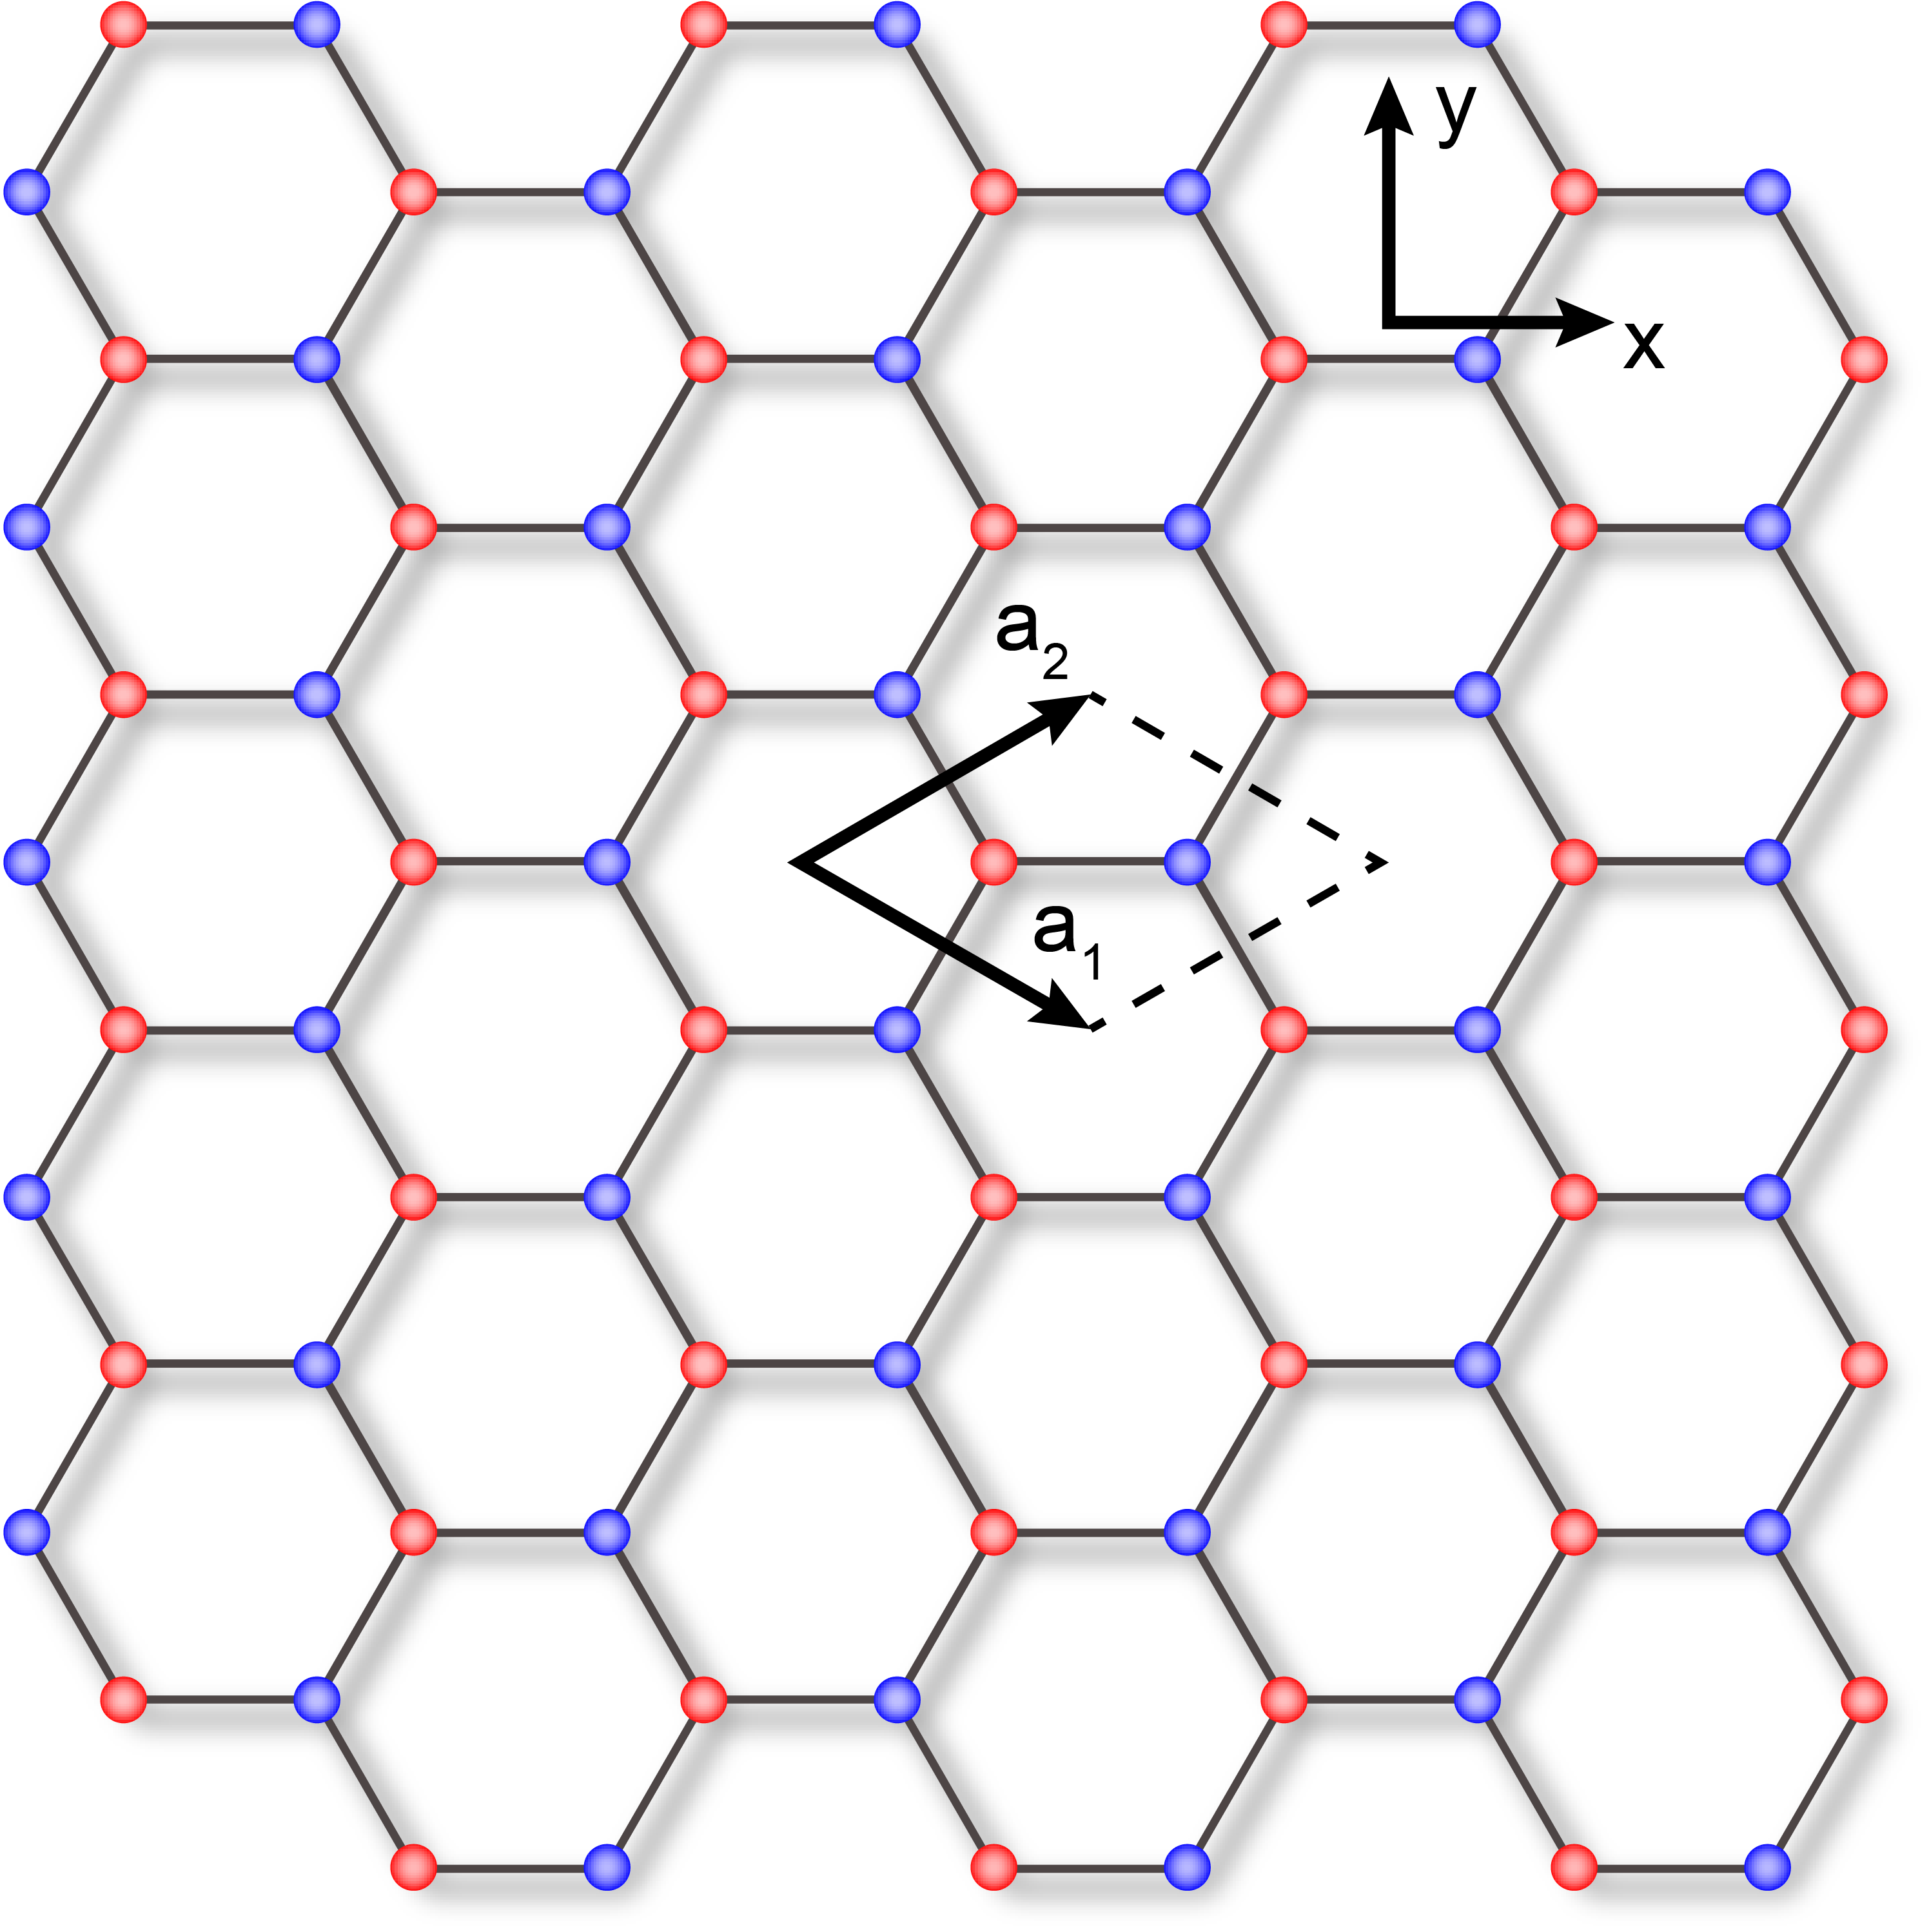
\includegraphics[width = 0.5\textwidth]{chapter2/graphene_unit_cell.png}
    \caption{The real-space structure of the graphene lattice. Vectors $\vec{a}_1$ and $\vec{a}_2$ define the unit cell, which contains two atoms, highlighted in red and blue.}
    \label{fig:graphene_unit_cell}
\end{figure}

In Figure \ref{fig:graphene_unit_cell} the unit cell is defined by the two lattice vectors $\vec{a}_1$ and $\vec{a}_2$. Each unit cell is comprised of two atoms. The honeycomb lattice can be thought of as to interpenetrating triangular sublattices. With that picture, the honeycomb unit cell contains one atom from each of the two sublattices, highlighted in Figure \ref{fig:graphene_unit_cell} as red (A) and blue (B). Each atom on the lattice contributes one conduction electron.

Using the coordinates defined in Figure \ref{fig:graphene_unit_cell}, the lattice vectors are defined, from the center of a honeycomb.

\begin{align}
    \vec{a}_1 &= \frac{3a}{2}\hat{i} + \frac{\sqrt{3}a}{2}\hat{j} \\
    \vec{a}_2 &= \frac{3a}{2}\hat{i} - \frac{\sqrt{3}a}{2}\hat{j}
\end{align}

Here $a$ is the carbon-carbon bond distance, \SI{1.42}{\angstrom} (CITE).

The reciprocal lattice vectors, $\vec{b}_1$ and $\vec{b}_2$ can now be found in the usual way.

\begin{equation}
    a_i \cdot b_j = 2\pi \delta_{ij}
\end{equation}

Here $\delta_{ij}$ is the Kronecker delta. The reciprocal lattice defined by $\vec{b}_1$ and $\vec{b}_2$ can be seen in Figure \ref{fig:graphene_k_space}.

\begin{align}
    \vec{b}_1 &= \frac{2\pi}{3a}\hat{i} + \frac{2\sqrt{3}\pi}{3a}\hat{j} \\
    \vec{b}_2 &= \frac{2\pi}{3a}\hat{i} - \frac{2\sqrt{3}\pi}{3a}\hat{j}
\end{align}

\begin{figure}
    \centering
    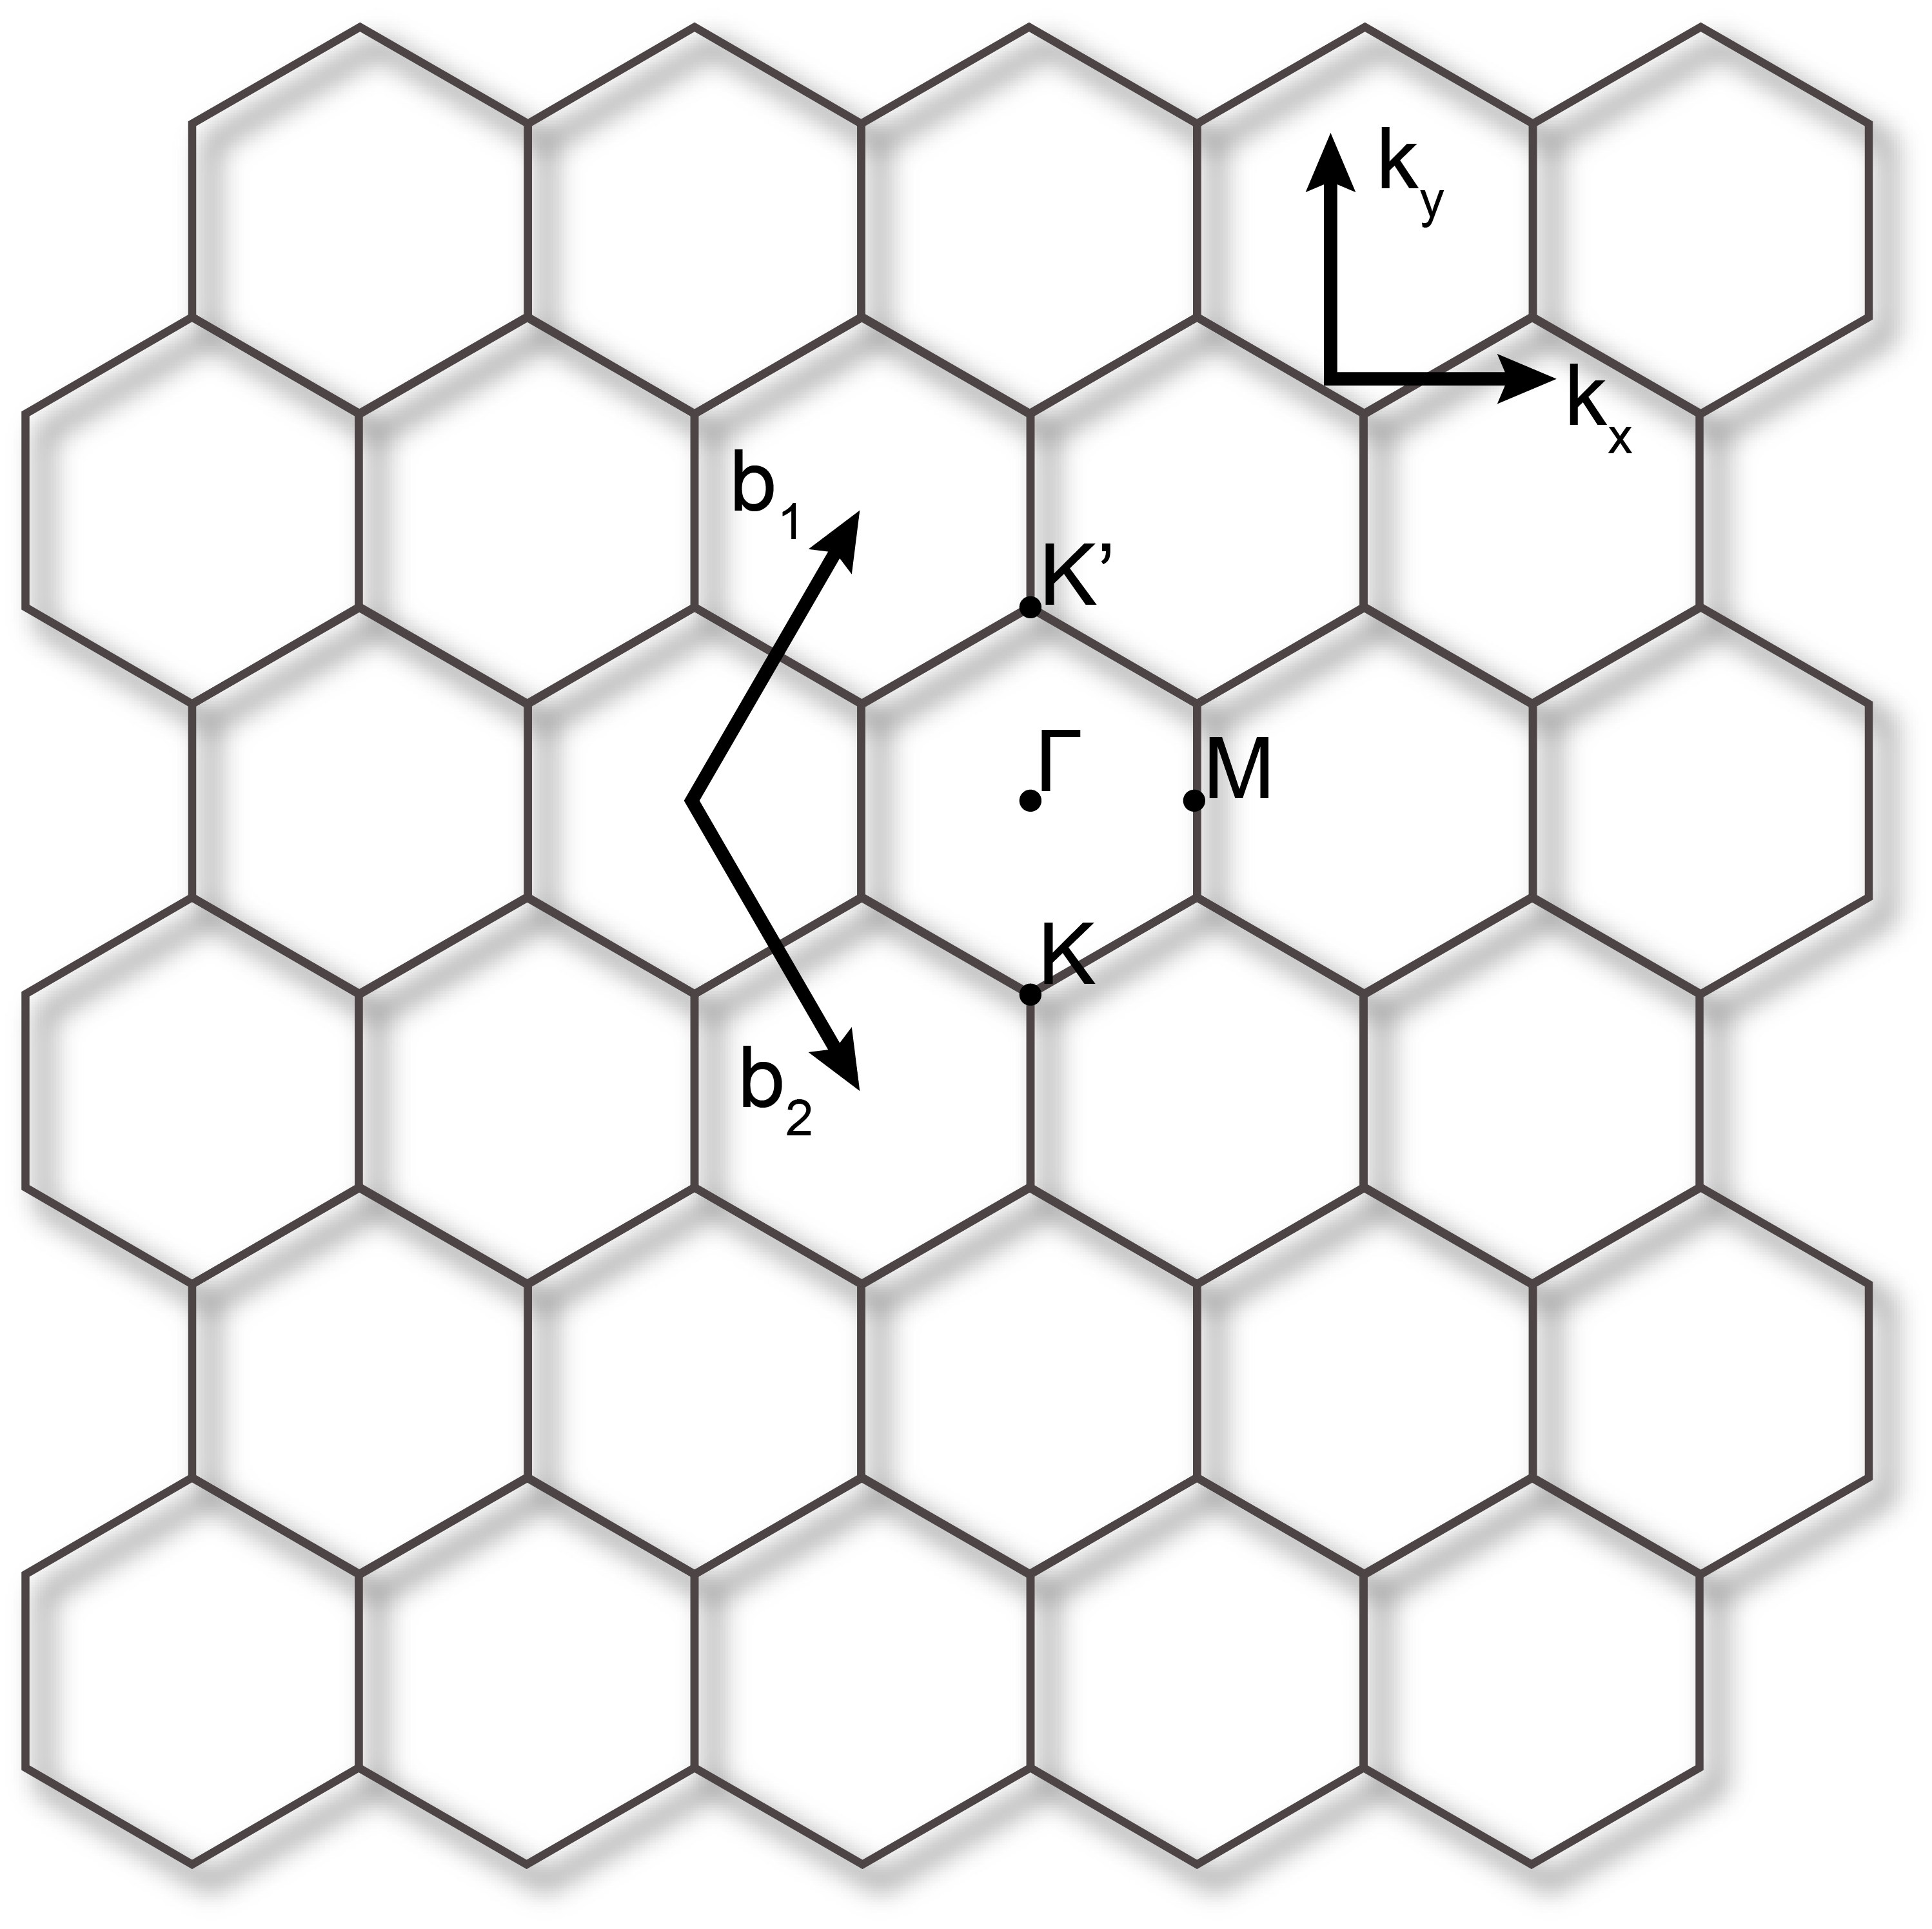
\includegraphics[width = 0.5\textwidth]{chapter2/graphene_k_space.png}
    \caption{The reciprocal lattice of graphene. Vectors $\vec{b}_1$ and $\vec{b}_2$ define the Brillouin zone. The high symmetry points $\Gamma$, $K$, $K'$, and $M$ are labeled.}
    \label{fig:graphene_k_space}
\end{figure}

The reciprocal lattice is also a honeycomb lattice, rotated 90 degrees from the real space lattice. The size of each Brillouin zone is defined by the reciprocal lattice vectors above. A few high symmetry points have been labelled in the figure. Of particular note are the three $K$ and three $K'$ points. As will be seen in the band structure calculation, these are the points at which the conduction and valence bands will meet to form the Dirac cones that give rise to graphene's interesting low energy conduction properties.

\subsection{Tight Binding Model}

The simplest way to calculate the low energy electronic band structure for graphene is using a nearest neighbor tight binding model, also known as a linear combination of atomic orbitals (CITE). In this model, each conduction electron is tightly bound to a lattice site with a small probability of hopping only to a nearest neighbor site. With this simple picture for electron conduction, one can find the lowest energy bands in graphene.

Given that the model deals with the motion of individual electrons and their wavefunctions at each atomic site, the goal will be to solve the time independent Schr\"{o}dinger equation.

\begin{equation}
    \hat{H}\Psi = \varepsilon\Psi
\end{equation}

$\Psi$ is a single particle wavefunction over the whole graphene lattice. As such, it can be written as a linear combination of Bloch wavefucntions.

\begin{align}
    u_A(\vec{r}) &= \frac{1}{\sqrt{N}}\sum_{\vec{r}_A}^{} e^{i\vec{k}\cdot\vec{r}_A} \phi_{2p_z}(\vec{r}-\vec{r}_A) \\
    u_B(\vec{r}) &= \frac{1}{\sqrt{N}}\sum_{\vec{r}_B}^{} e^{i\vec{k}\cdot\vec{r}_B} \phi_{2p_z}(\vec{r}-\vec{r}_B)
\end{align}

These two functions represent Bloch waves localized on the A and B sublattices, respectively. With these definitions the full single-particle wavefunction can be rewritten as follows:

\begin{equation}
    \Psi = C_A u_A + C_B u_B
\end{equation}

$C_{A(B)}$ represents the amplitude of the wavefunction on the A(B) sublattice. With all of the above definitions the time independent Schr\"{o}dinger equation can be rewritten in a matrix form:

\begin{equation} 
\label{eq:TISE}
    \begin{pmatrix} H_{AA} & H_{AB} \\ H_{BA} & H_{BB} \end{pmatrix} \begin{pmatrix} C_A \\ C_B \end{pmatrix} = \varepsilon \begin{pmatrix} S_{AA} & S_{AB} \\ S_{BA} & S_{BB} \end{pmatrix} \begin{pmatrix} C_A \\ C_B \end{pmatrix}
\end{equation}

Where:

\begin{align}
\label{eq:matel}
    H_{ij} &= \braket{u_i | H | u_j} \\
    S_{ij} &= \braket{u_i | u_j}
\end{align}

For simplicity, the rest of this calculation will assume $\braket{u_i | u_j} = \delta_{ij}$. Meaning, there is no overlap of the two Bloch wavefunctions and that each of the wave functions is already properly normalized. Rewriting Equation \ref{eq:TISE} yields:

\begin{equation}
\label{eq:secular}
    \begin{pmatrix} H_{AA}-\varepsilon & H_{AB} \\ H_{BA} & H_{BB}-\varepsilon \end{pmatrix} \begin{pmatrix} C_A \\ C_B \end{pmatrix} = 0
\end{equation}

Non-trival solutions to Equation \ref{eq:secular} exist only when:

\begin{equation}
\label{eq:eigenvals}
    \begin{vmatrix} H_{AA}-\varepsilon & H_{AB} \\ H_{BA} & H_{BB}-\varepsilon \end{vmatrix} = 0
\end{equation}

Solving equation \ref{eq:eigenvals} gives the energy eigenvalues in terms of the matrix elements defined in equation \ref{eq:matel}.

\begin{equation}
\label{eq:simple_bands}
    \varepsilon = H_{AA} \pm \lvert H_{AB} \rvert
\end{equation}

Where the relations $H_{AA} = H_{BB}$ and $H_{AB} = {H^*}_{BA}$ were used.

In order to obtain a useful expression for the energy bands in terms of the electron momentum $\vec{k}$, Equation \ref{eq:simple_bands} must be simplified using the expressions for the Bloch wavefunctions. 

\begin{align}
    H_{AA} &= \frac{1}{N} \sum_{\vec{r}_A}^{} \sum_{\pvec{r}'_A}^{} e^{i \vec{k}\cdot(\vec{r}_A - \pvec{r}'_A)} \int \phi^*_{2p_z}(\vec{r}-\vec{r}_A) \hat{H} \phi_{2p_z}(\vec{r}-\pvec{r}'_A) \, d^3\vec{r} \label{eq:overlap_AA} \\
    H_{AB} &= \frac{1}{N} \sum_{\vec{r}_A}^{} \sum_{\vec{r}_B}^{} e^{i \vec{k}\cdot(\vec{r}_A - \vec{r}_B)} \int \phi^*_{2p_z}(\vec{r}-\vec{r}_A) \hat{H} \phi_{2p_z}(\vec{r}-\vec{r}_B) \, d^3\vec{r} \label{eq:overlap_AB}
\end{align}

The summation in Equation \ref{eq:overlap_AA} can be evaluated to yield:

\begin{equation}
\label{eq:pz_energy}
    H_{AA} = \int \phi^*_{2p_z}(\vec{r}-\vec{r}_A) \hat{H} \phi_{2p_z}(\vec{r}-\vec{r}_A) \, d^3\vec{r} = \varepsilon_{p_z}
\end{equation}

Where $\varepsilon_{p_z}$ is the energy of a single electron on a $p_z$ orbital. For the sake of simplicity, the rest of this chapter will assume $\varepsilon_{p_z} = 0$. 

In order to simplify Equation \ref{eq:overlap_AB} it is useful to define the vectors pointing from an atom on the B sublattice to its three nearest neighbors on the A sublattice.

\begin{align}
    \vec{\delta}_1 &= -a\hat{i} \nonumber \\
    \vec{\delta}_2 &= \frac{a}{2}\hat{i} - \frac{\sqrt{3}}{2}a\hat{j} \label{eq:deltas} \\
    \vec{\delta}_3 &= \frac{a}{2}\hat{i} + \frac{\sqrt{3}}{2}a\hat{j} \nonumber 
\label{eq:deltas}
\end{align}

With these definitions Equation \ref{eq:overlap_AB} can be rewritten as:

\begin{equation}
\label{eq:AB_simple}
    \hat{H}_{AB} = \sum_{i=1}^{3} e^{i\vec{k}\cdot\vec{\delta}_i} \int \phi^*_{2p_z}(\vec{r}) \hat{H} \phi_{2p_z}(\vec{r}- \vec{\delta}_i) \, d^3\vec{r}
\end{equation}

Since the exact form of the Hamiltonian is not known, the integral in Equation \ref{eq:AB_simple} cannot be evaluated. However, the integral clearly represents the overlap between the wavefunction of an electron in a $p_z$ orbital on the A lattice and its nearest neighbor on the B lattice. With that in mind, the hopping amplitude $t$ is defined:

\begin{equation}
\label{eq:hopping_amp}
    t = \int \phi^*_{2p_z}(\vec{r}) \hat{H} \phi_{2p_z}(\vec{r}-\vec{\delta}_i) \, d^3\vec{r}
\end{equation}

Note, there is only one hopping amplitude, independent of the index $i$, since the distance between all nearest neighbors, $\lvert \delta_i \rvert$, is the same. With this definition, the overlap integral can be rewritten once more.

\begin{equation}
\label{eq:AB_final}
    H_{AB} = t \sum_{i=1}^{3} e^{i\vec{k}\cdot\vec{\delta}_i}
\end{equation}

Equation \ref{eq:AB_final} can be combined with the assumption that the onsite energy can be set to zero, $\varepsilon_{p_z} = 0$ to give the final effective Hamiltonian for this model.

\begin{equation}
\label{eq:effective_H}
    \hat{H} = \begin{pmatrix} 0 & t \sum_{i}^{} e^{i\vec{k}\cdot\vec{\delta}_i} \\  t \sum_{i}^{} e^{-i\vec{k}\cdot\vec{\delta}_i} & 0 \end{pmatrix}
\end{equation}

Using these same results in Equation \ref{eq:simple_bands} gives the two lowest energy bands in terms of the hopping amplitude, $t$. 

\begin{equation}
    \varepsilon(\vec{k}) = \pm t \left| \sum_{i}^{} e^{i \vec{k}\cdot\vec{\delta}_i} \right|
    \label{eq:f_k}
\end{equation}

\begin{equation}
    \varepsilon(\vec{k}) = \pm t \sqrt{ 1 + 4\cos\left(\frac{3a}{2}k_x\right)\cos\left(\frac{\sqrt{3}a}{2}k_y\right) + 4\cos^{2}\left(\frac{\sqrt{3}a}{2}k_y\right)} \label{eq:bands}
\end{equation}    

These two bands can be seen in Figure \ref{fig:graphene_bands}. Note that the plot does not assume  $S_{ij} = \braket{u_i | u_j} = \delta_{ij}$, which introduces some asymmetry in the valence and conduction bands.

\begin{figure}
    \centering
    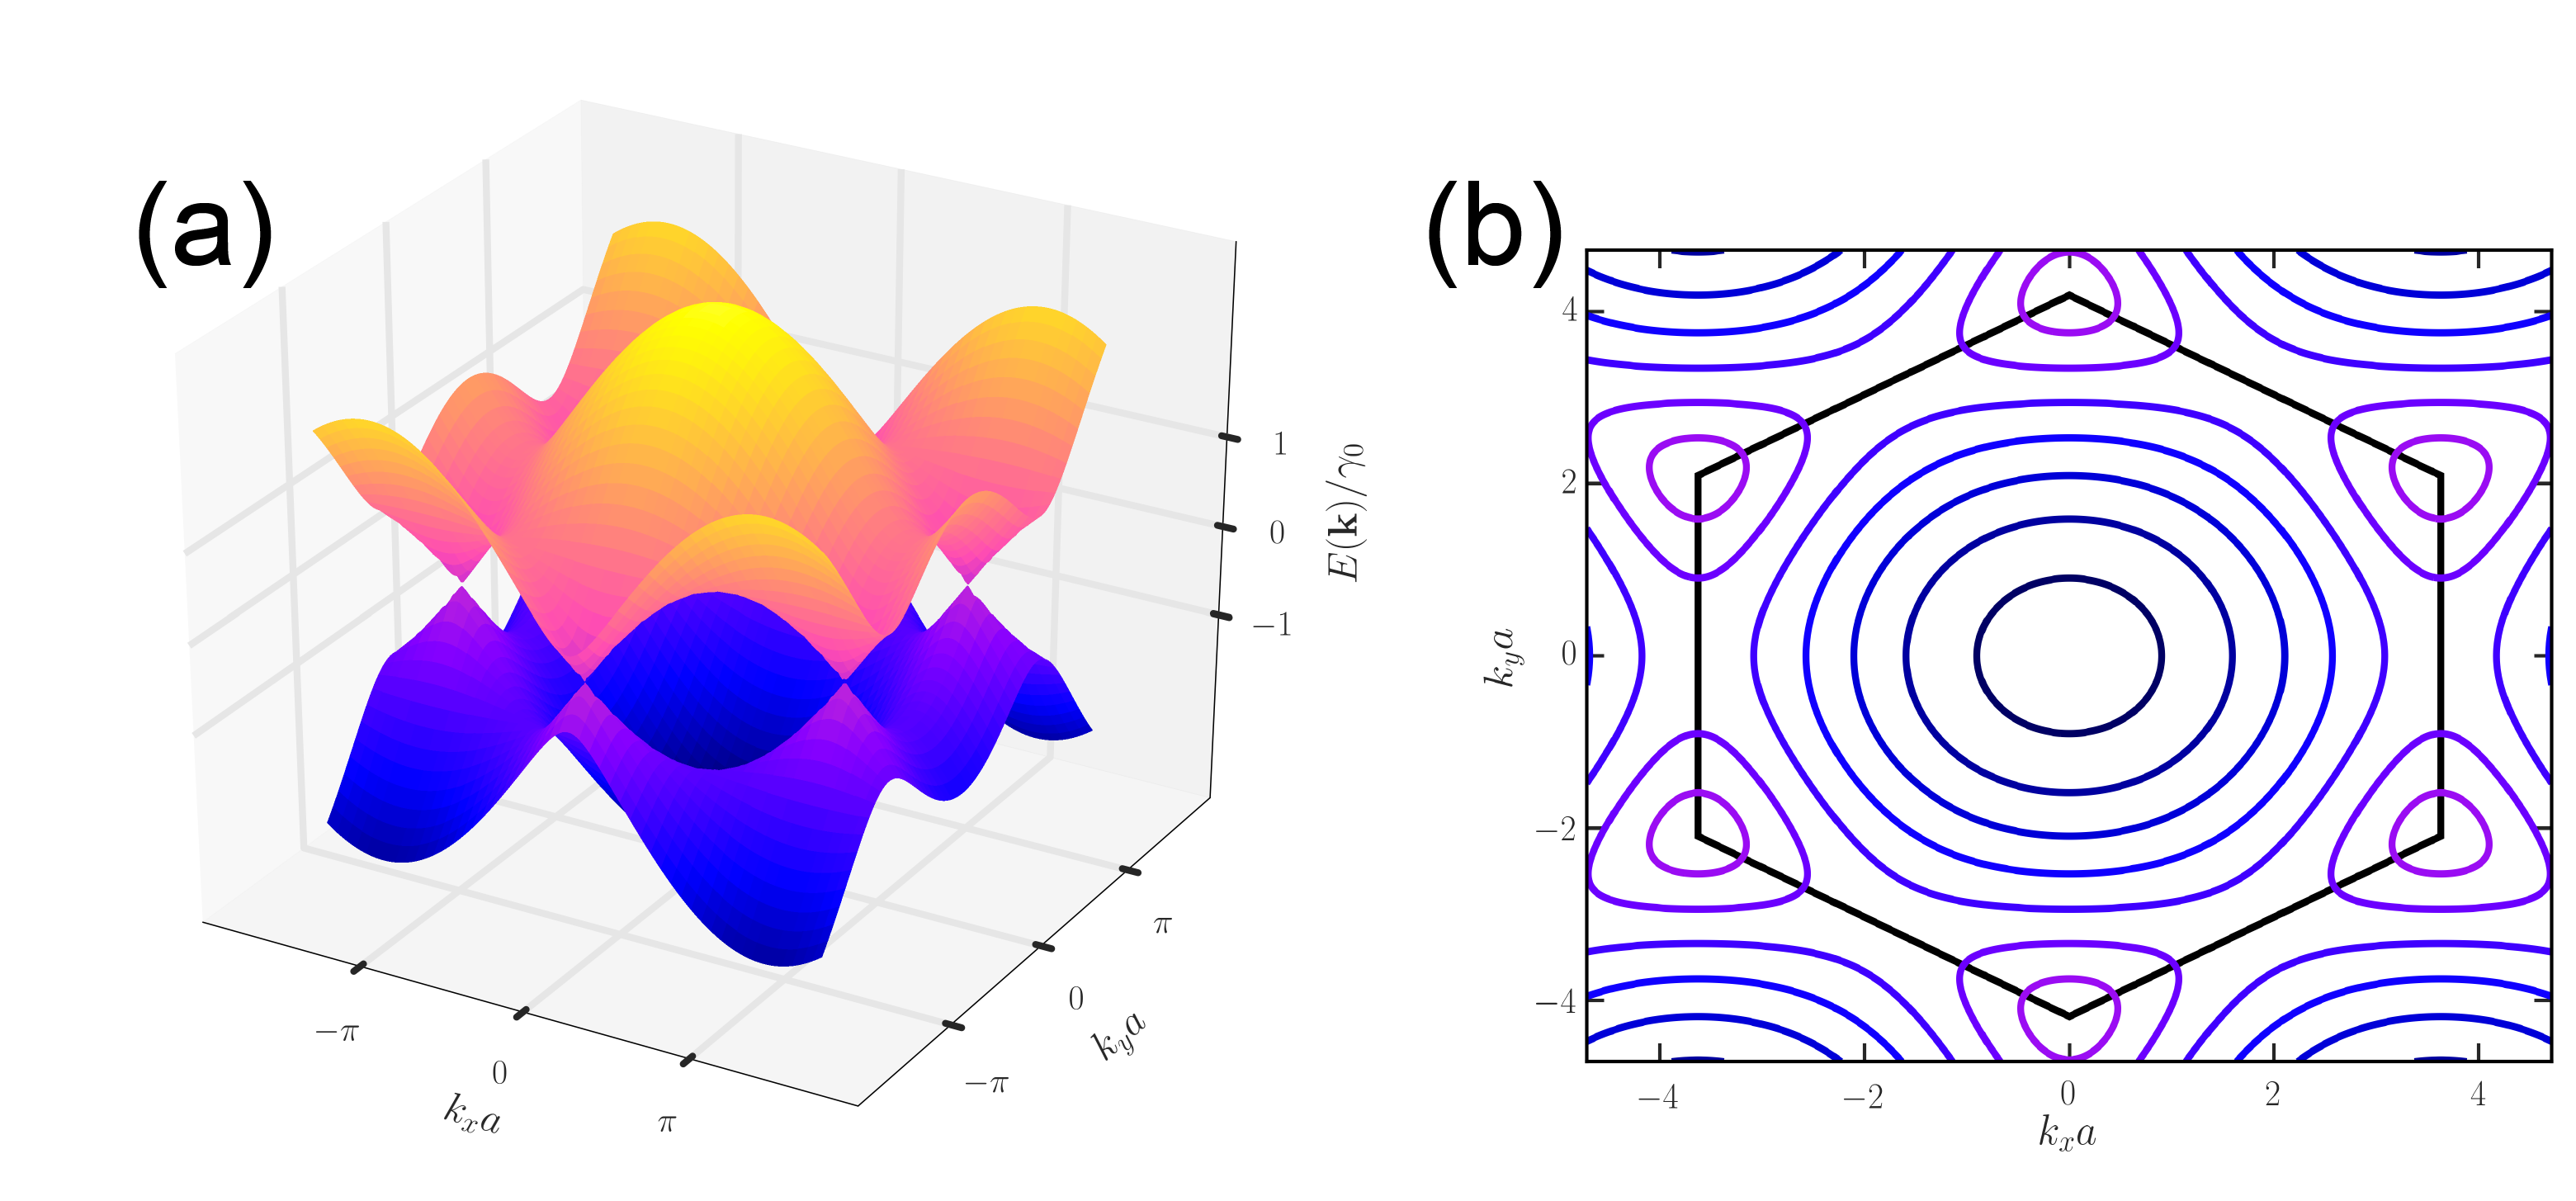
\includegraphics[width = 1.0\textwidth]{chapter2/graphene_band_fig.png}
    \caption{(a) The $\pi$-bands of graphene calculated using a nearest neighbor tight binding model. (b) A contour plot of the upper band with the first Brillouin zone drawn. The bands meet at the three $K$ and three $K'$ points at the vertices of the Brillouin zone.}
    \label{fig:graphene_bands}
\end{figure}

\subsection{Low Energy Bandstructure of Graphene}

For low energy electronic excitations, conduction will be dominated by the bandstructure near the $K$ and $K'$ points. There are only two inequivalent points, since the other 4 are equivalent by the symmetry of the honeycomb lattice. Consider the two points located at:

\begin{align}
    \vec{K} &= 0\hat{i} - \frac{4\pi}{3\sqrt{3}a}\hat{j} \\
    \pvec{K}' &= -\vec{K} = 0\hat{i} + \frac{4\pi}{3\sqrt{3}a}\hat{j}
\end{align}

To get the low-energy dispersion relation, expand the Hamiltonian in Equation \ref{eq:effective_H} around the $K$ point.

\begin{equation}
    \vec{k} = \vec{K} + \vec{q}
\end{equation}

\begin{equation}
\label{eq:approx_HK}
    \hat{H} \approx -i\frac{3at}{2} \begin{pmatrix} 0 & q_x+iq_y\\ -(q_x-iq_y)& 0 \end{pmatrix}
\end{equation}

Similarly, expanding around the $K'$ point yields:

\begin{equation}
\label{eq:approx_HKp}
    \hat{H} \approx -i\frac{3at}{2} \begin{pmatrix} 0 & q_x-iq_y\\ -(q_x+iq_y)& 0 \end{pmatrix}
\end{equation}

By defining $v_f \equiv {3at}/{2\hbar}$, using the standard Pauli matrices, and rotating the phase, Equations \ref{eq:approx_HK} and \ref{eq:approx_HKp} can be written in a more suggestive form. 

\begin{align}
    \hat{H}_K &= \hbar v_f \vec{\sigma}\cdot\vec{q} \label{eq:chiral_HK} \\
    \hat{H}_{K'} &= \hbar v_f \pvec{\sigma}^*\cdot\vec{q} \nonumber
\end{align}

These Hamiltonians describe massless Dirac fermions in 2D. This is clear in the low-energy dispersion relation.

\begin{equation}
\label{eq:massless_disp}
    \varepsilon(\vec{q}) = \pm\hbar v_f q
\end{equation}

It is also important to note, in Equation \ref{eq:chiral_HK}, that the sublattice structure has lead to a spin-1/2 degree of freedom. This degree of freedom is known as the valley degeneracy or pseudospin. 

A useful consequence of the pseudospin is the reduction in scattering in graphene and carbon nanotubes. The reduced backscattering is a result of the introduction of an additional symmetry to the system. This reduction in scattering leads to unusually high mobilities and long spin coherence lengths in both materials. The increased spin coherence length make carbon nanotubes suitable for spin-based devices.

\section{Electronic Bandstructure of Carbon Nanotubes} 

Now that the bandstructure a graphene sheet has been calculated, finding the electronic bandstructure of various carbon nanotubes is as simple as applying a few boundary conditions.

The structure of a carbon nanotube can be completely described by its chiral vector.

\begin{align}
    \vec{C}_h &= m\vec{a}_1 + n\vec{a}_2 \label{eq:chiral_vec} \\
    \vec{C}_h &= \frac{3}{2}(n+m)a\hat{i} + \frac{\sqrt{3}}{2}(n-m)a\hat{j} \nonumber
\end{align}

This vector describes how to roll a graphene sheet to form the nanotube. The tube is formed by rolling the graphene sheet such that the tip and tail of $\vec{C}_h$ meet. The indices $(n,m)$ describe the type of nanotube that is formed. A tube where $0<m<n$ is known as chiral, $m=n$ is an armchair nanotube, and $m=0$ is a zig-zag nanotube. Armchair and zig-zag tubes get their names from the shape of the carbon bonds on the edge of the unit cell.

\begin{figure}
    \centering
    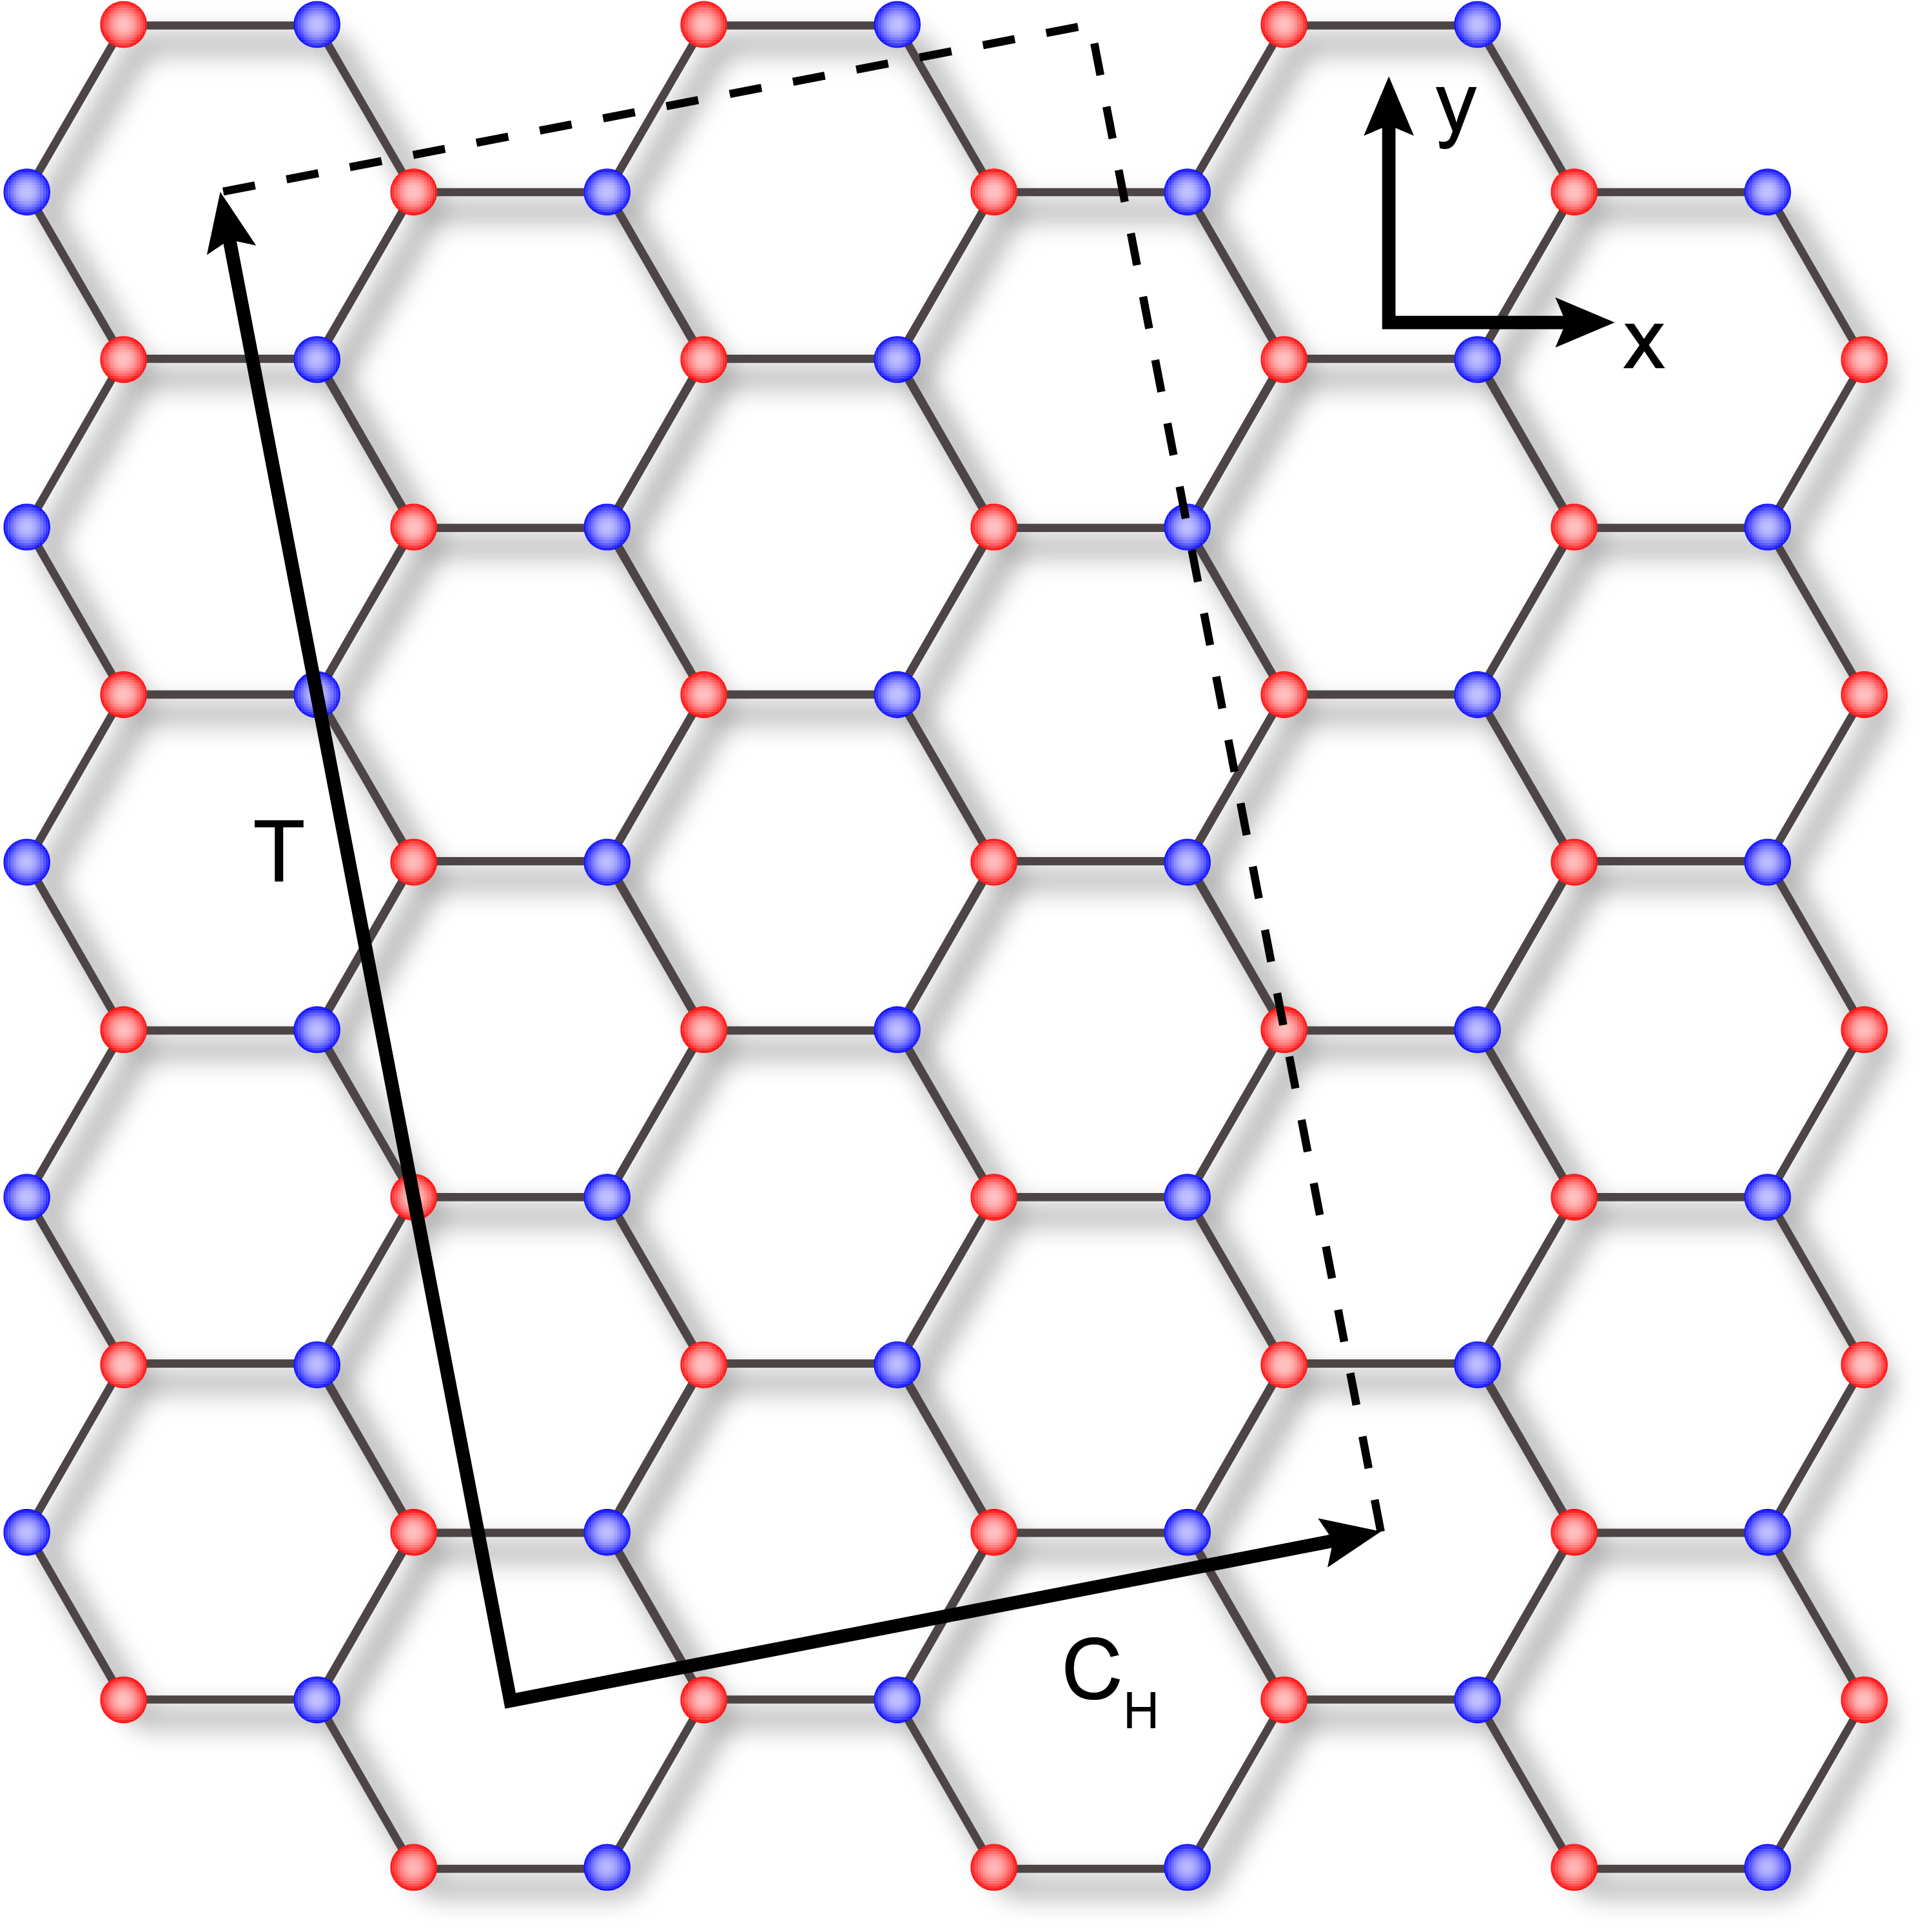
\includegraphics[width = 0.5\textwidth]{chapter2/nanotube_unit_cell.png}
    \caption{The real-space structure of a carbon nanotube. The nanotube unit cell is defined by the vectors $\vec{C}_h$ and $\vec{T}$}
    \label{fig:cnt_unit_cell}
\end{figure}

An example of a chiral (2,1) nanotube unit cell can be seen in Figure \ref{fig:cnt_unit_cell}. The unit cell is defined by the chiral vector $\vec{C_h}$ and the translation vector $\vec{T}$, which is defined as:

\begin{equation}
    \vec{T} = t_1\vec{a}_1 + t_2\vec{a}_2 \label{eq:translation}
\end{equation}
    
where $t_1 = (2m+n)/d_R, t_2 = (2n-m)/d_R$ and $d_R = gcd(2n+m, 2m+n)$. These two vectors can be used to calculate a few basic properties of the nanotube. The diameter of the nanotube is found from the chiral vector:

\begin{equation}
    d = \left| \vec{C}_h \right|/\pi = \frac{\sqrt{3}a}{\pi}\sqrt{n^2+nm+m^2}
    \label{eq:cnt_diameter}
\end{equation}

The number of graphene unit cells contained in the nanotube unit cell is also easily calculated:

\begin{equation}
    N = \frac{\left| \vec{C}_h \times \vec{T} \right|}{\left| \vec{a}_1 \times \vec{a}_2 \right|} = \frac{2}{d_R}\sqrt{n^2+nm+m^2}
    \label{eq:cnt_N}
\end{equation}

Knowing the number of graphene unit cells contained in the nanotube unit cell yields a lot of useful information about the band structure. There are 2N carbon atoms in the nanotube unit cell and N conduction electrons. There will be 2N bands (one for each carbon atom) that will be half-filled, just like the graphene bandstructure.

The reciprocal lattice vectors for the carbon nanotube defined by $(n,m)$ can be found in the usual way.

\begin{align}
    \vec{C}_h\cdot\vec{K}_1 &= \vec{T}\cdot\vec{K}_2 = 2\pi \nonumber \\
    \vec{C}_h\cdot\vec{K}_2 &= \vec{T}\cdot\vec{K}_1 = 0 \label{eq:cnt_recip}
\end{align}
    
\begin{align}
    \vec{K}_1 &= -\frac{(t_2 \vec{b}_1 - t_1 \vec{b}_2)}{N} \nonumber \\
    \vec{K}_2 &= \frac{(m \vec{b}_1 - n \vec{b}_2)}{N} \label{eq:K1_K2}
\end{align}

The reciprocal space of the unrolled nanotube is quantized along $\vec{K}_1$ and continuous along $\vec{K}_2$. This means the electron momentum $k$ in the nanotube is quantized along the direction of $C_h$. These quantized 'cutting lines' define the electronic bands in the carbon nanotube:

\begin{equation}
    \vec{k}\cdot\vec{C}_h = 2\pi\mu
\end{equation}

Where $\mu$ is an integer from $1-N/2$ to $N/2$ and $\mu=0$ cuts through the $\Gamma$ point at the center of the graphene Brillouin zone. The structure of the nanotube reciprocal lattice, definied by $K_1$ and $K_2$ can be seen in Figure \ref{fig:cnt_k_space}. 

\begin{figure}
    \centering
    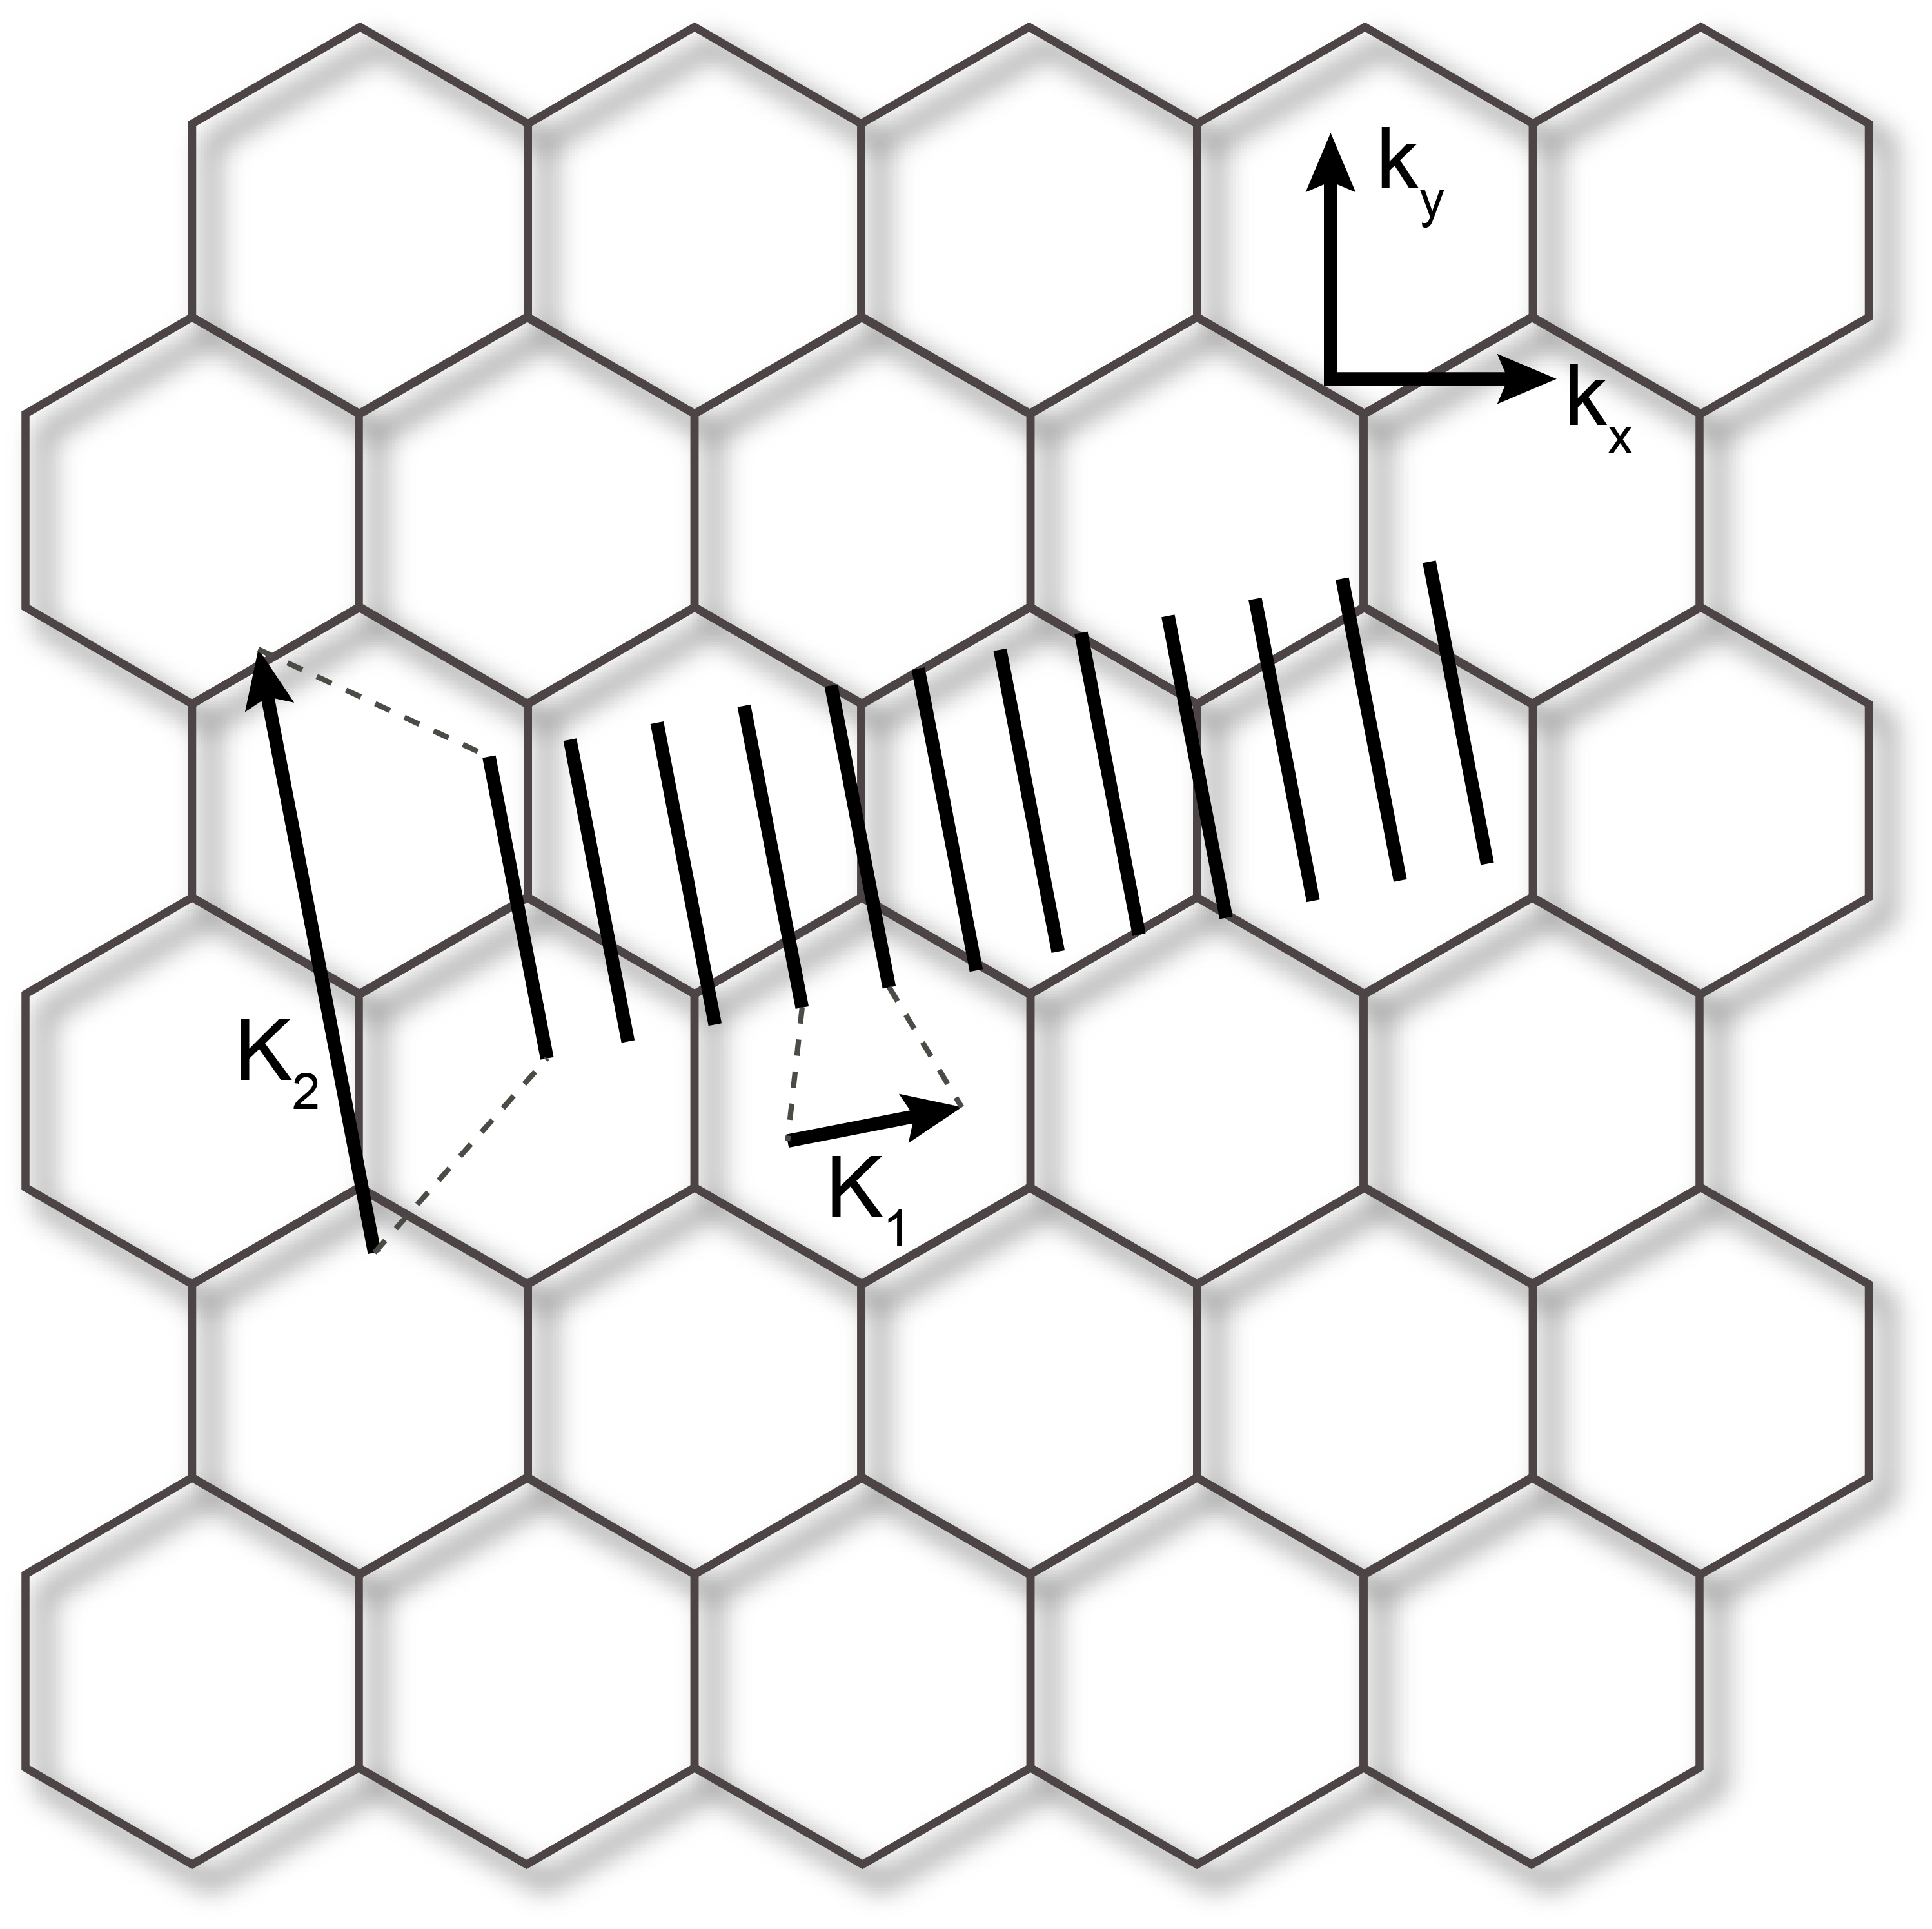
\includegraphics[width = 0.5\textwidth]{chapter2/nanotube_k_space.png}
    \caption{The reciprocal lattice of a carbon nanotube, defined by the vectors $K_1$ and $K_2$}
    \label{fig:cnt_k_space}
\end{figure}

With all of these definitions, the electron momentum in the carbon nanotube can be rewritten.

\begin{equation}
    \vec{k} = \mu\vec{K}_1 + k_{\parallel}\frac{\vec{K}_2}{|\vec{K}_2|}
    \label{eq:k_quant}
\end{equation}

The bands for a generic nanotube can be found by simply inserting this definition for the momentum into the graphene bands derived in Equation \ref{eq:bands}. 

\subsection{Types of Carbon Nanotubes}

The electronic properties of a carbon nanotube are determined by its chirality, $(n,m)$. If one of the cutting lines, as seen in Figure \ref{fig:cnt_k_space}, passes through a $K$ or $K'$ point, the nanotube will have a metallic band structure. Like in graphene, two of the valence and conduction bands will meet at discrete points at the Fermi energy. If this is not the case, and none of the cutting lines pass through a $K$ or $K'$ point, the nanotube will be semiconducting with a bandgap determined by the chirality.

To determine if a nanotube is semiconducting or metallic, one can look at the projection of $\vec{K}$, the vector pointing to a $K$ point in the graphene Brillouin zone, and $\vec{K}_1$, the nanotube reciprocal lattice vector.

\begin{equation}
    \frac{\vec{K}\cdot\vec{K}_1}{\vec{K}_1\vec{K}_1} = \frac{(2n+m)}{3} 
    \label{eq:metallic_condition}
\end{equation}

From Equation \ref{eq:metallic_condition}, it is clear that a nanotube is metallic if $(n-m)\bmod3 = 0$. There are two other cases, where $(n-m)\bmod3 = 1$ or $(n-m)\bmod3 = 2$. Each of these results in a semiconducting nanotube. Based on these results, in a collection of nanotubes with random chirality, $(n,m)$, there will be roughly $1/3$ metallic and $2/3$ semiconducting nanotubes.

Figure \ref{fig:cnt_types} shows the full bandstructure of a metallic $(5,5)$ armchair nanotube and a semiconducting $(4,2)$ chiral nanotube. These have 20 and 56 bands, respectively.

\begin{figure}
    \centering
    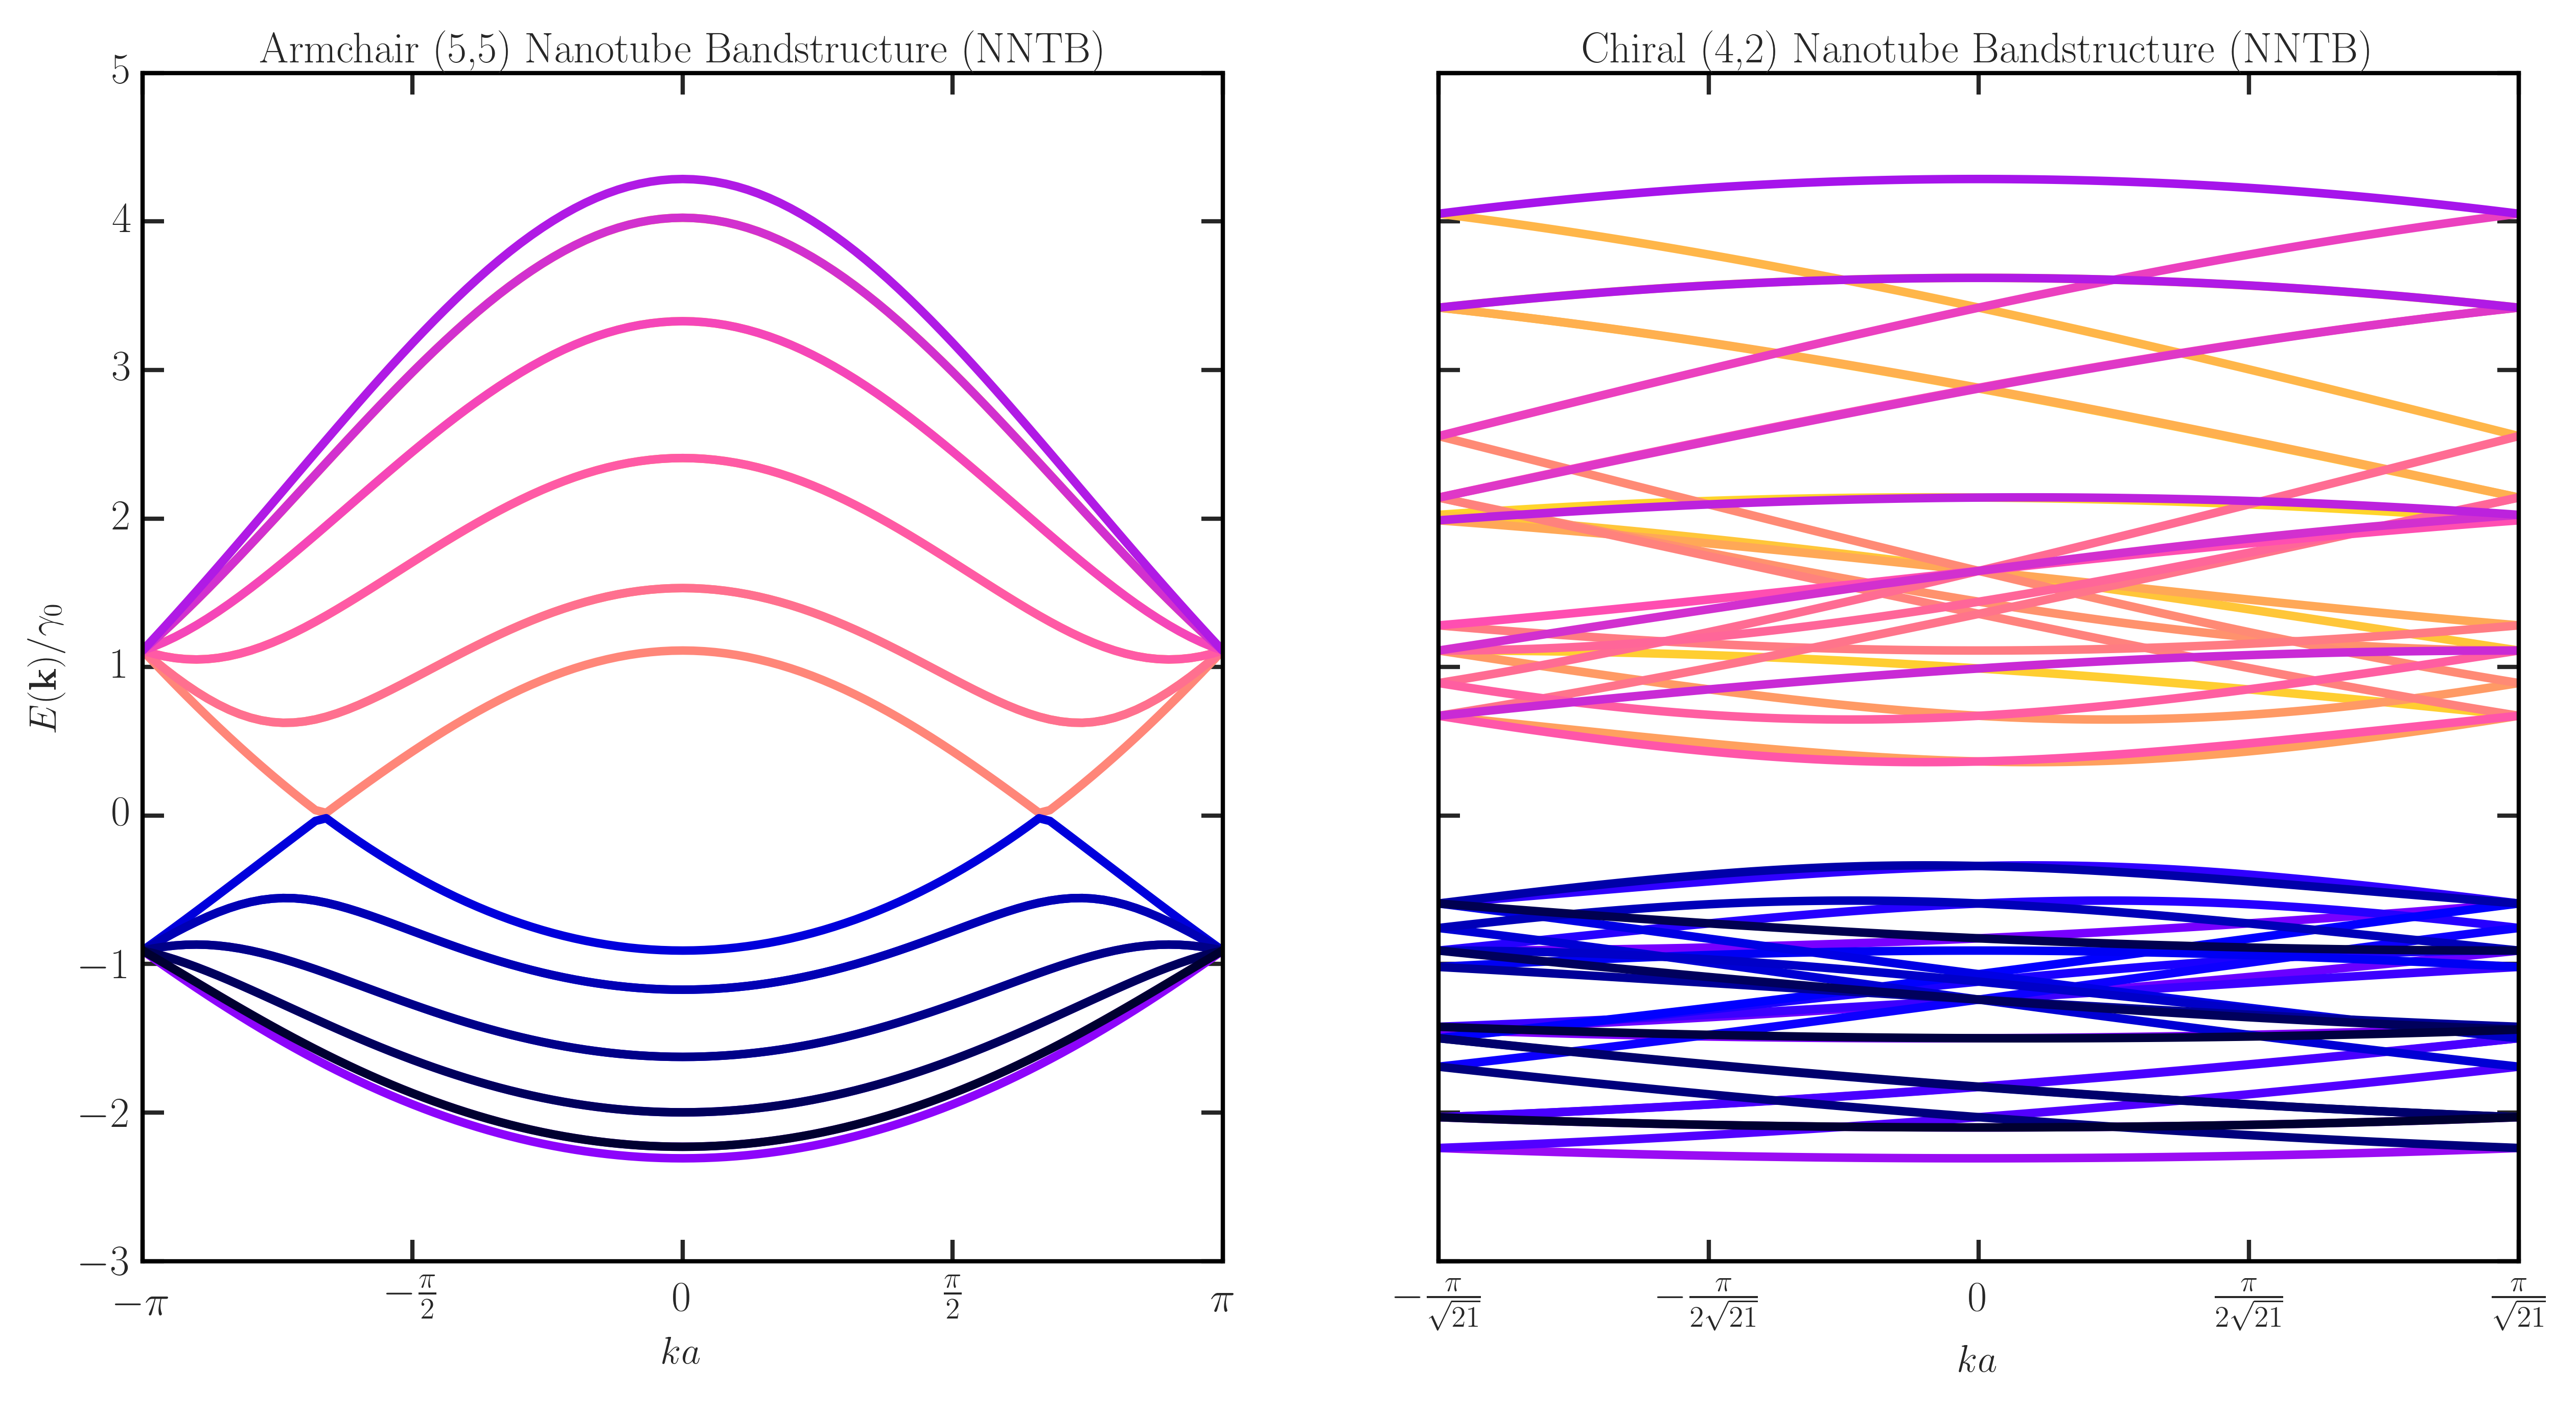
\includegraphics[width = 1.0\textwidth]{chapter2/cnt_types.png}
    \caption{Two types of carbon nanotube bandstructure. The left plot shows a metallic $(5,5)$ armchair nanotube. The right plot shows a semiconducting $(4,2)$ chiral nanotube.}
    \label{fig:cnt_types}
\end{figure}


\subsection{Low Energy Bandstructure of Carbon Nanotubes}

To calculate the full set of bands for a generic nanotube $(n,m)$ is cumbersome. The basic proprties for a generic nanotube can be more easily calculated by first expanding the graphene bands about the $K$ and $K'$ points as in Equation \ref{eq:massless_disp}, then using the quantized momentum derived in Equation \ref{eq:k_quant}. Doing this yields the low energy dispersion relation for a generic carbon nanotube:

\begin{equation}
    \varepsilon_{\mu}(k) = \pm\frac{2\hbar v_f}{d}\sqrt{\left(\frac{m-n}{3} - \mu\right)^2 + \left(\frac{kd}{2}\right)^2}
    \label{eq:low_e_cnt}
\end{equation}

Where $\mu$ is the band index, $d$ is the nanotube diameter, and k is the electron momentum along the nanotube axis. Looking at the first term in parentheses, it is clear that the nanotube will be metallic if $(m-n)/3$ is an integer. In that case, there will be some integer $\mu$ for which the valence and conduction bands meet at the Fermi energy. This is consistent with the condition derived previously for metallic and semiconducting chiral vectors. Using that information, the low energy bandstructure can be written as:

\begin{align}
    \varepsilon(k) &= \pm\left(\frac{1}{2}E_g(n,m) + \frac{\hbar^2}{2m^*}k^2\right) \\
    \varepsilon(k) &= \pm\hbar v_f k
\end{align}

These are the approximate bandstructures at low energy. Semiconducting nanotubes have a bandgap, $E_g(n,m)$ dependent on the chirality, and an effective mass $m^*$ dependent on the lowest band curvature. Metallic nanotubes maintain the massless Dirac fermion properties found in graphene at low energies.

\section{Carbon Nanotube Field Effect Transistors}

The simplest device that one can make with a carbon nanotube is a field effect transistor. A nanotube is placed, or grown, on a silicon substrate capped with an insulating silicon dioxide layer. Source and drain contacts are then made to the nanotube. The completed three terminal device consists of the source, drain, and a doped silicon substrate serves as the gate, with a silicon dioxide layer acting as the gate dielectric. A schematic of such a device is seen in Figure \ref{fig:nanotube_fet}

\begin{figure}
    \centering
    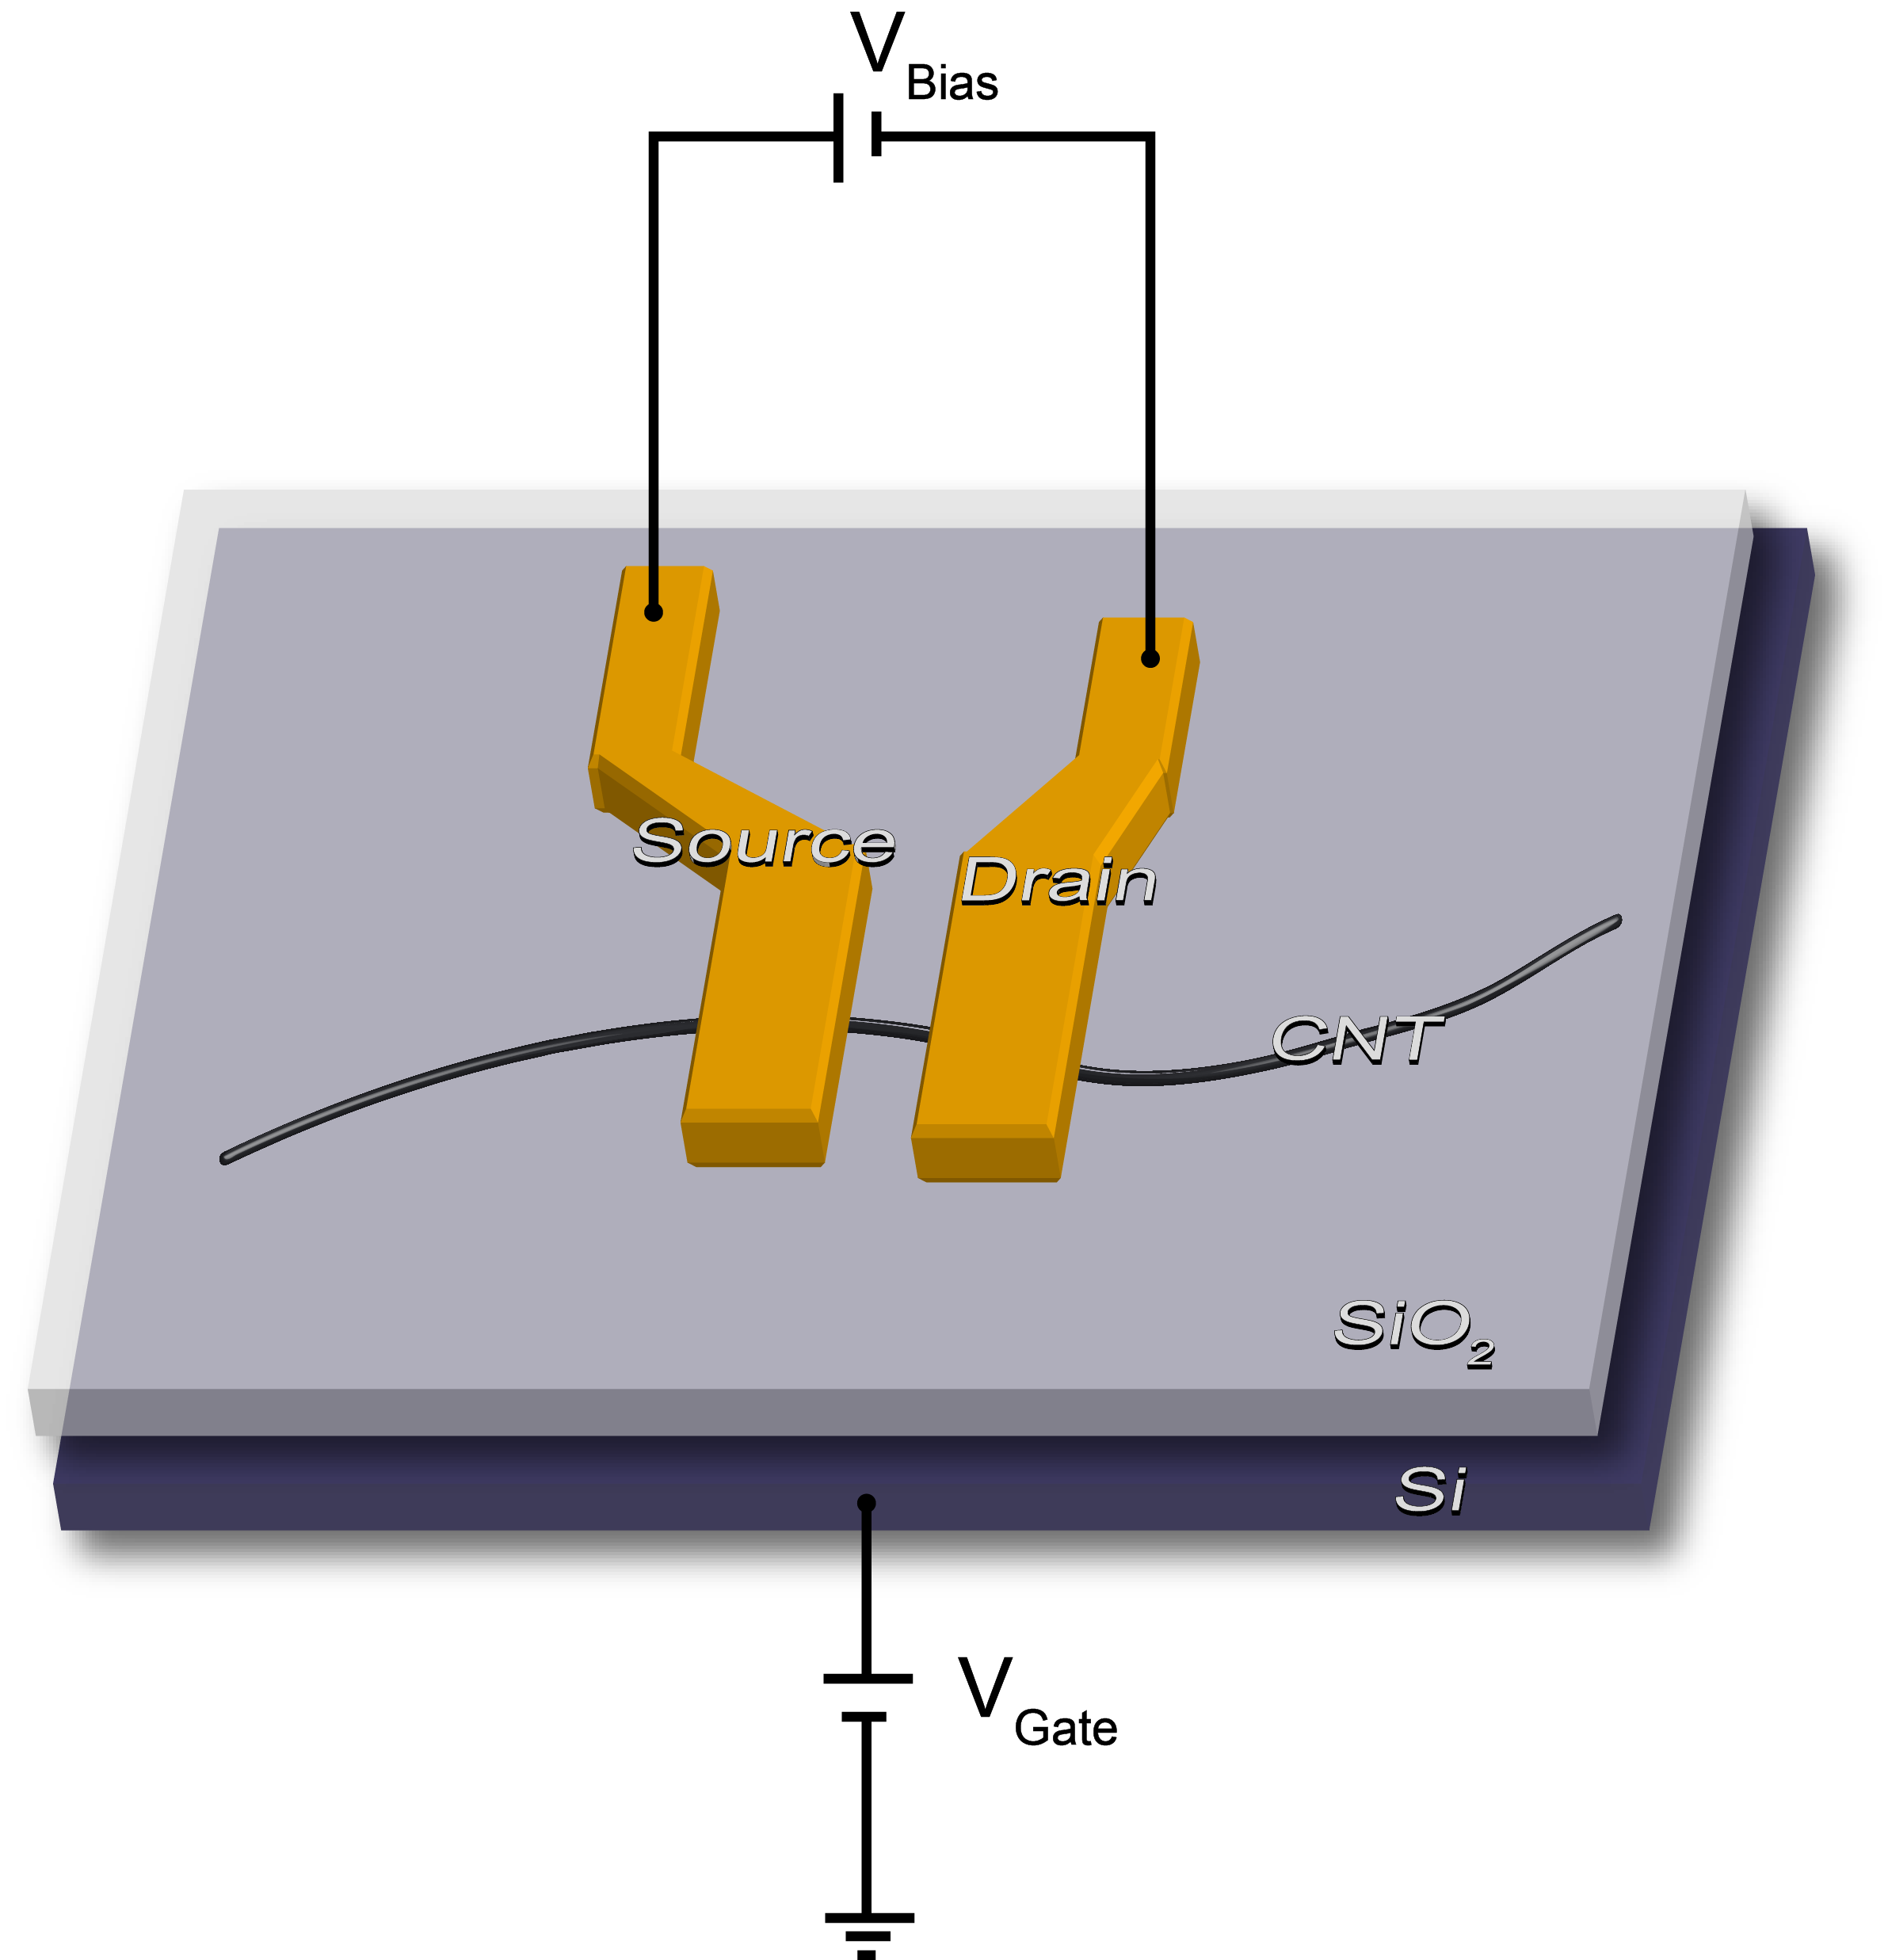
\includegraphics[width = 0.5\textwidth]{chapter2/nanotube_FET_device.png}
    \caption{Schematic of a carbon nanotube field effect transistor.}
    \label{fig:nanotube_fet}
\end{figure}

Measurements on carbon nanotube field effect transistors (CNTFETs) depend on the type of carbon nanotube that has been contacted.

\begin{figure}
    \centering
    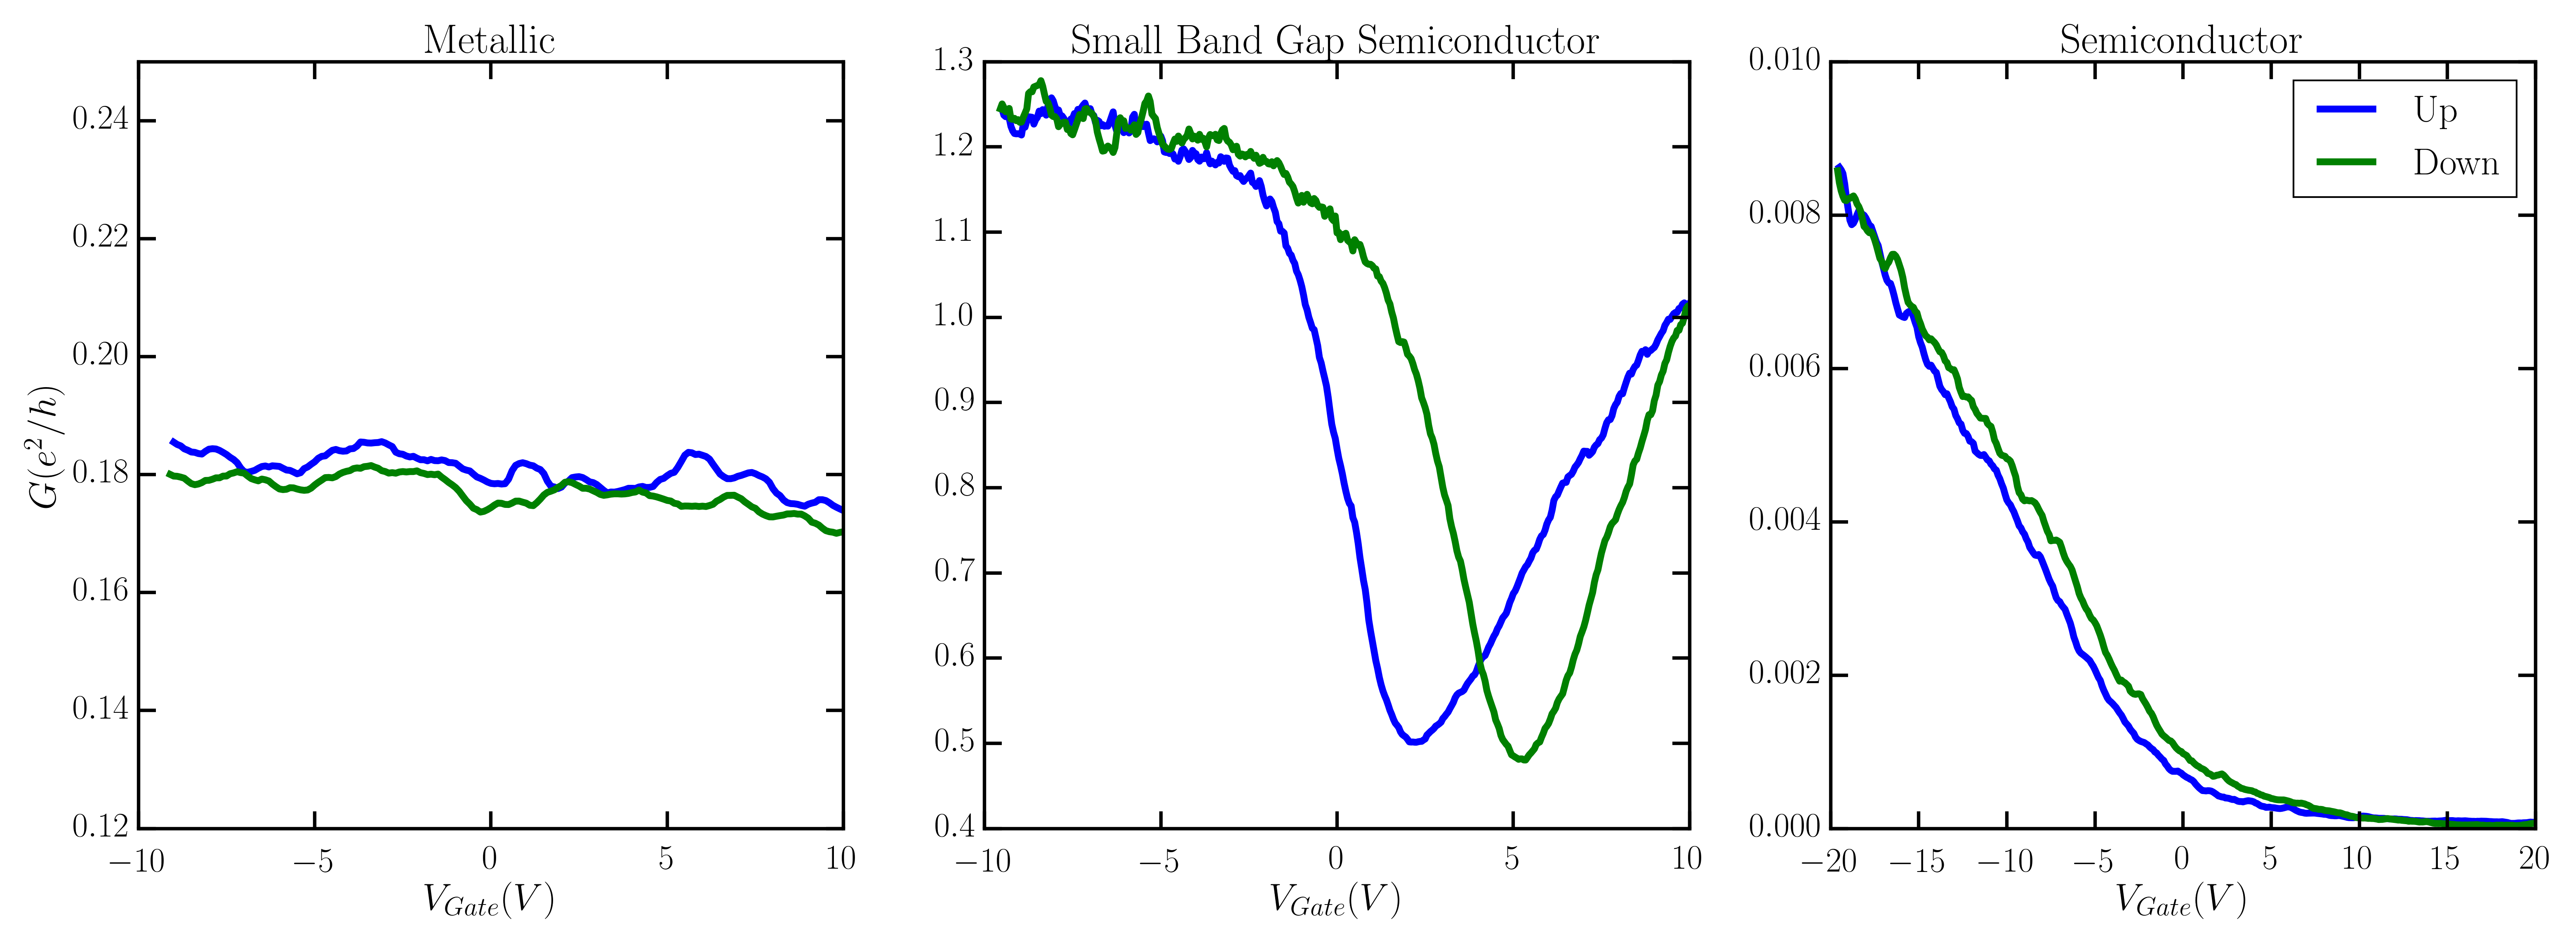
\includegraphics[width=1.0\textwidth]{chapter2/fet_measurements.png}
    \caption{Current versus gate voltage characteristics for three typs of CNTFET.}
    \label{fig:fet_measurements}
\end{figure}

\begin{figure}
    \centering
    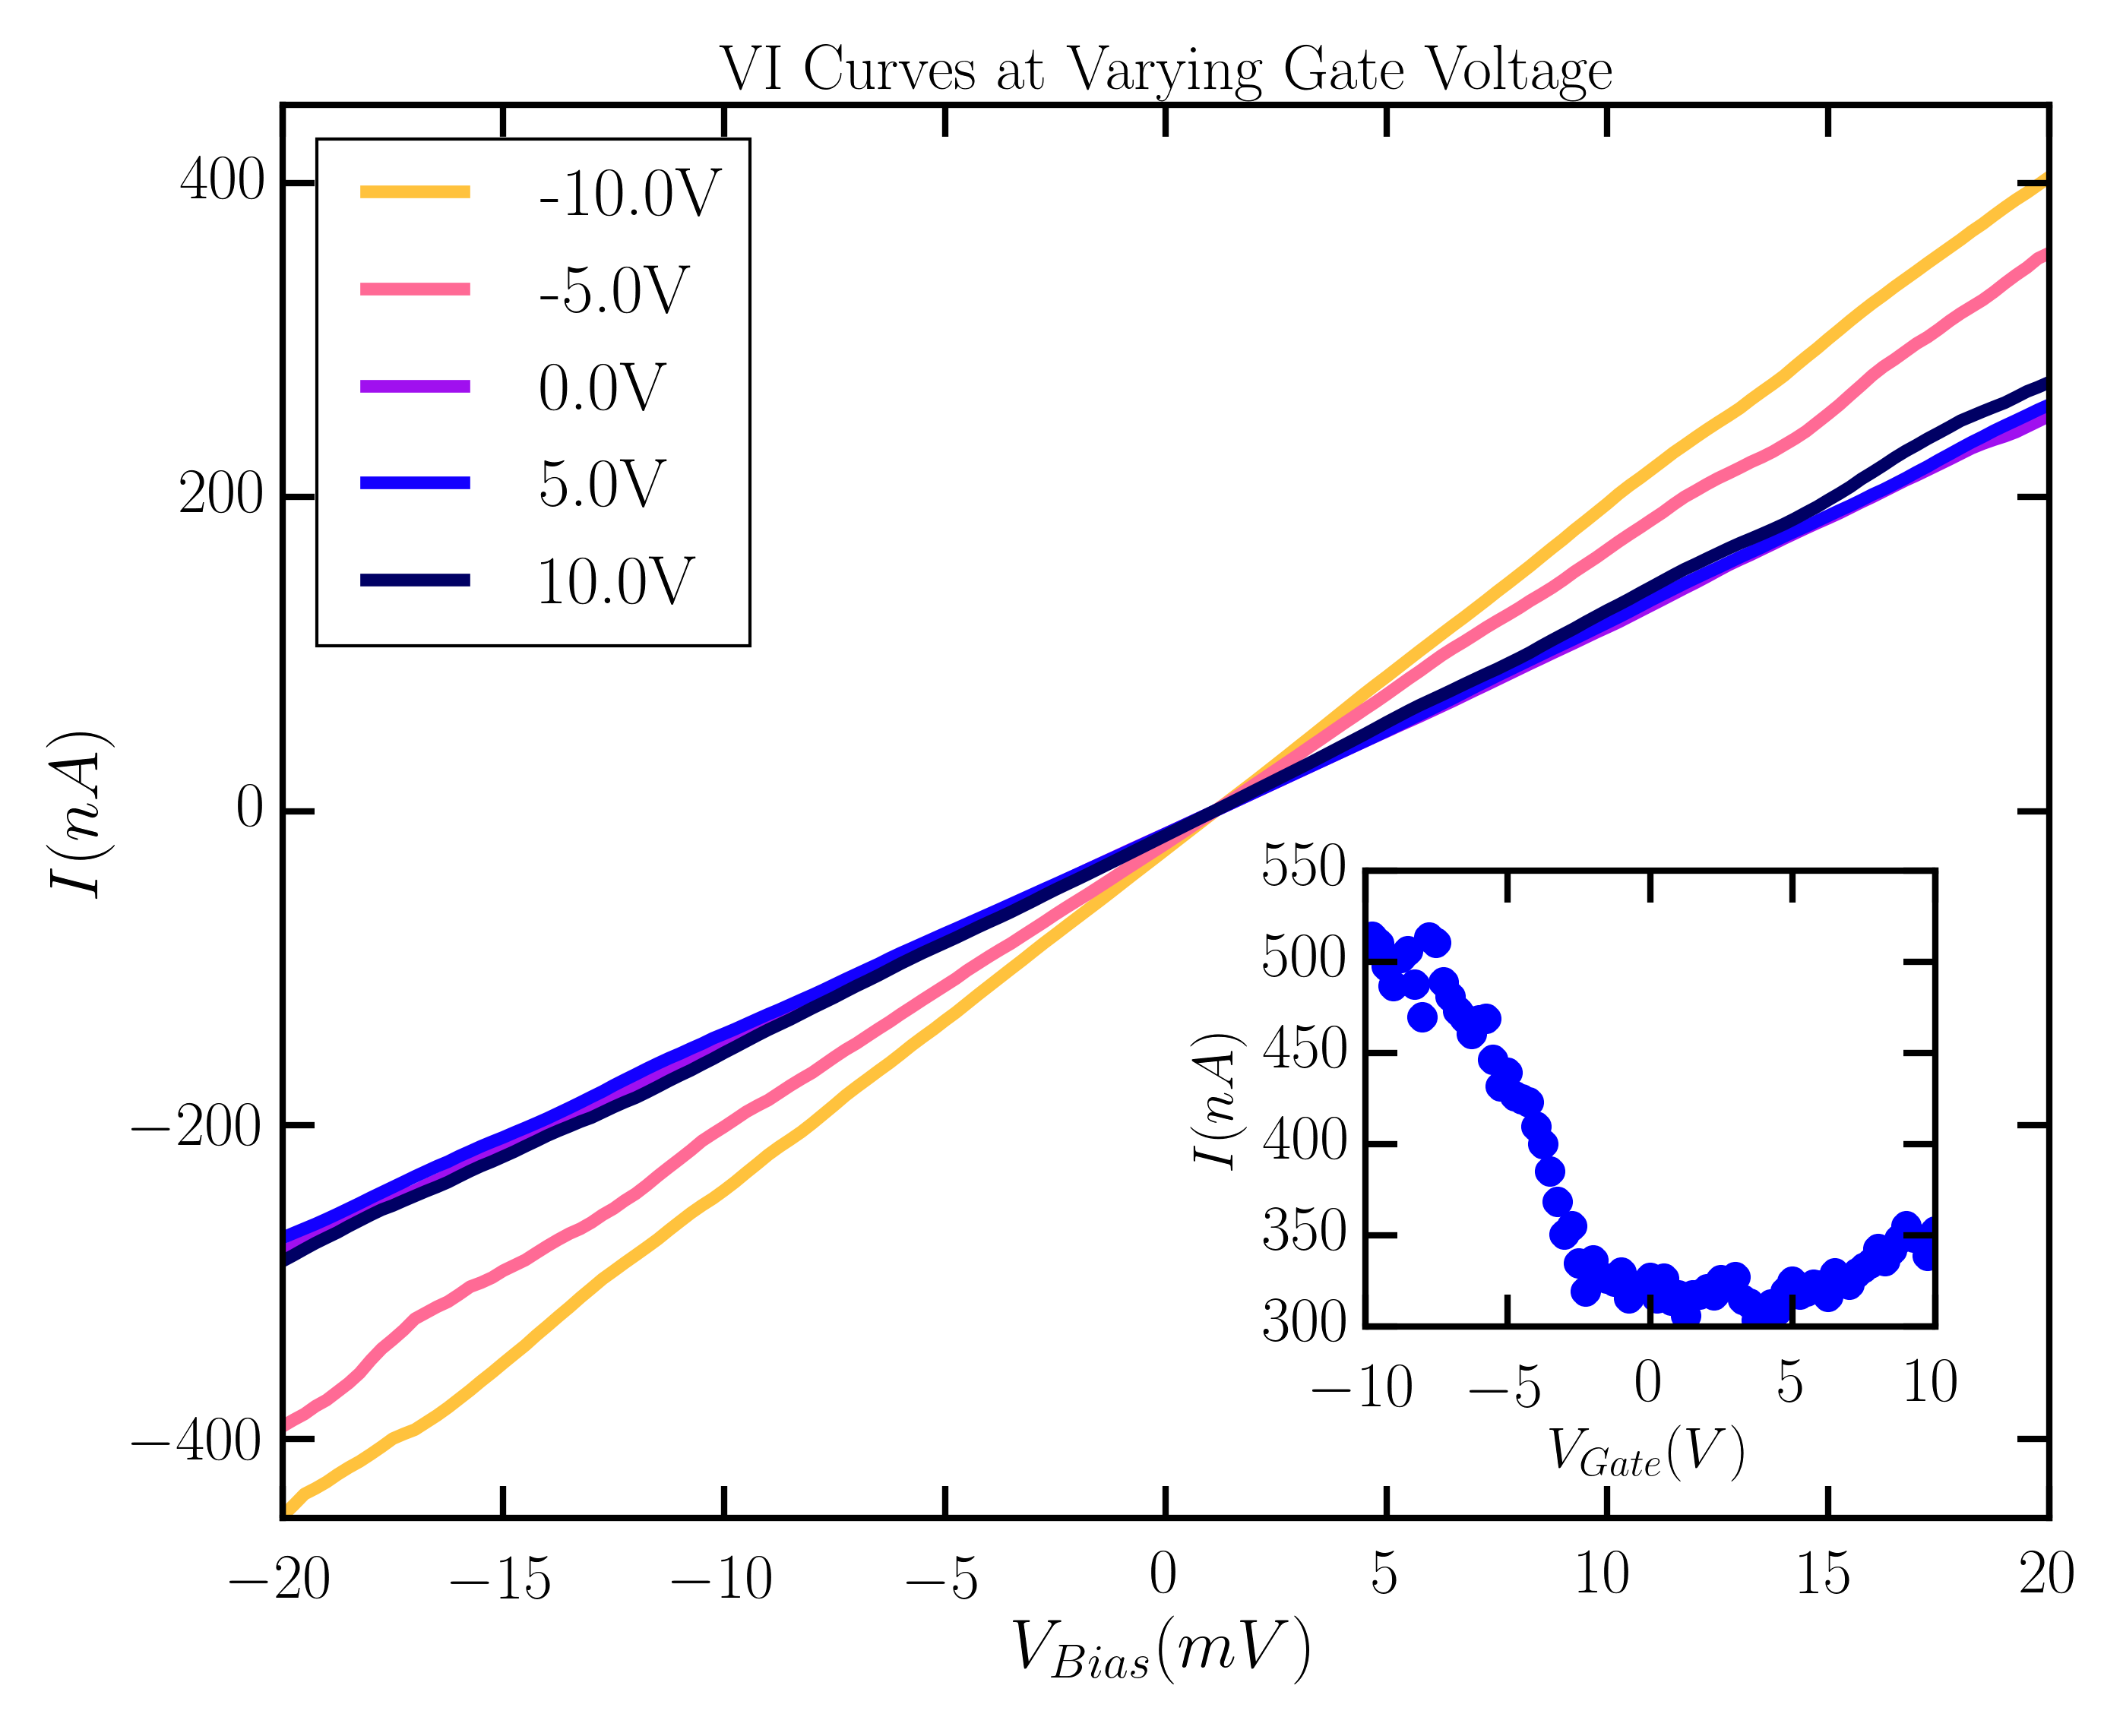
\includegraphics[width=0.7\textwidth]{chapter2/transistor_curves.png}
    \caption{IV characteristics of a typical small band gap semiconducting CNTFET. The current saturates at higher bias voltage, but is not typically measured due to avalanche breakdown of the devices. Inset: Current versus gate at a fixed bias for the same device.}
    \label{transistor_curves.png}
\end{figure}

Metallic source/drain contacts typically form Schottky barriers with carbon nanotubes. The polarity of the resulting CNTFET is thus determined by the relation between the work function of the contact material and nanotube. For metals with a relatively high work function, such as Pd, Ti, Cr, and Co, the devices are expected to be p-type. Metals with a lower work function, such as Al, Mg, and Sc, can produce n-type transistors. However, many of these low work function metals also happen to have a very poor wetability on the nanotube surface, which leads to large contact resistances, making the devices very difficult to fabricate and measure.

\section{Carbon Nanotube Quantum Dots}

When cooled to low temperatures ($\lesssim \SI{10}{\kelvin}$), the device drawn in Figure \ref{fig:nanotube_fet} exhibits quantum mechanical behavior. For a sufficiently short channel length ($L \lesssim \SI{500}{\nano\meter}$), electrons become confined within the carbon nanotube and behave like quantum mechanical particles in a box. This device is called a quantum dot. The resistance versus temperature plot in Figure \ref{fig:CNT_RT} shows the sharp increase in resistance as the tunneling through the device is suppressed at low temperatures. 

\begin{figure}
    \centering
    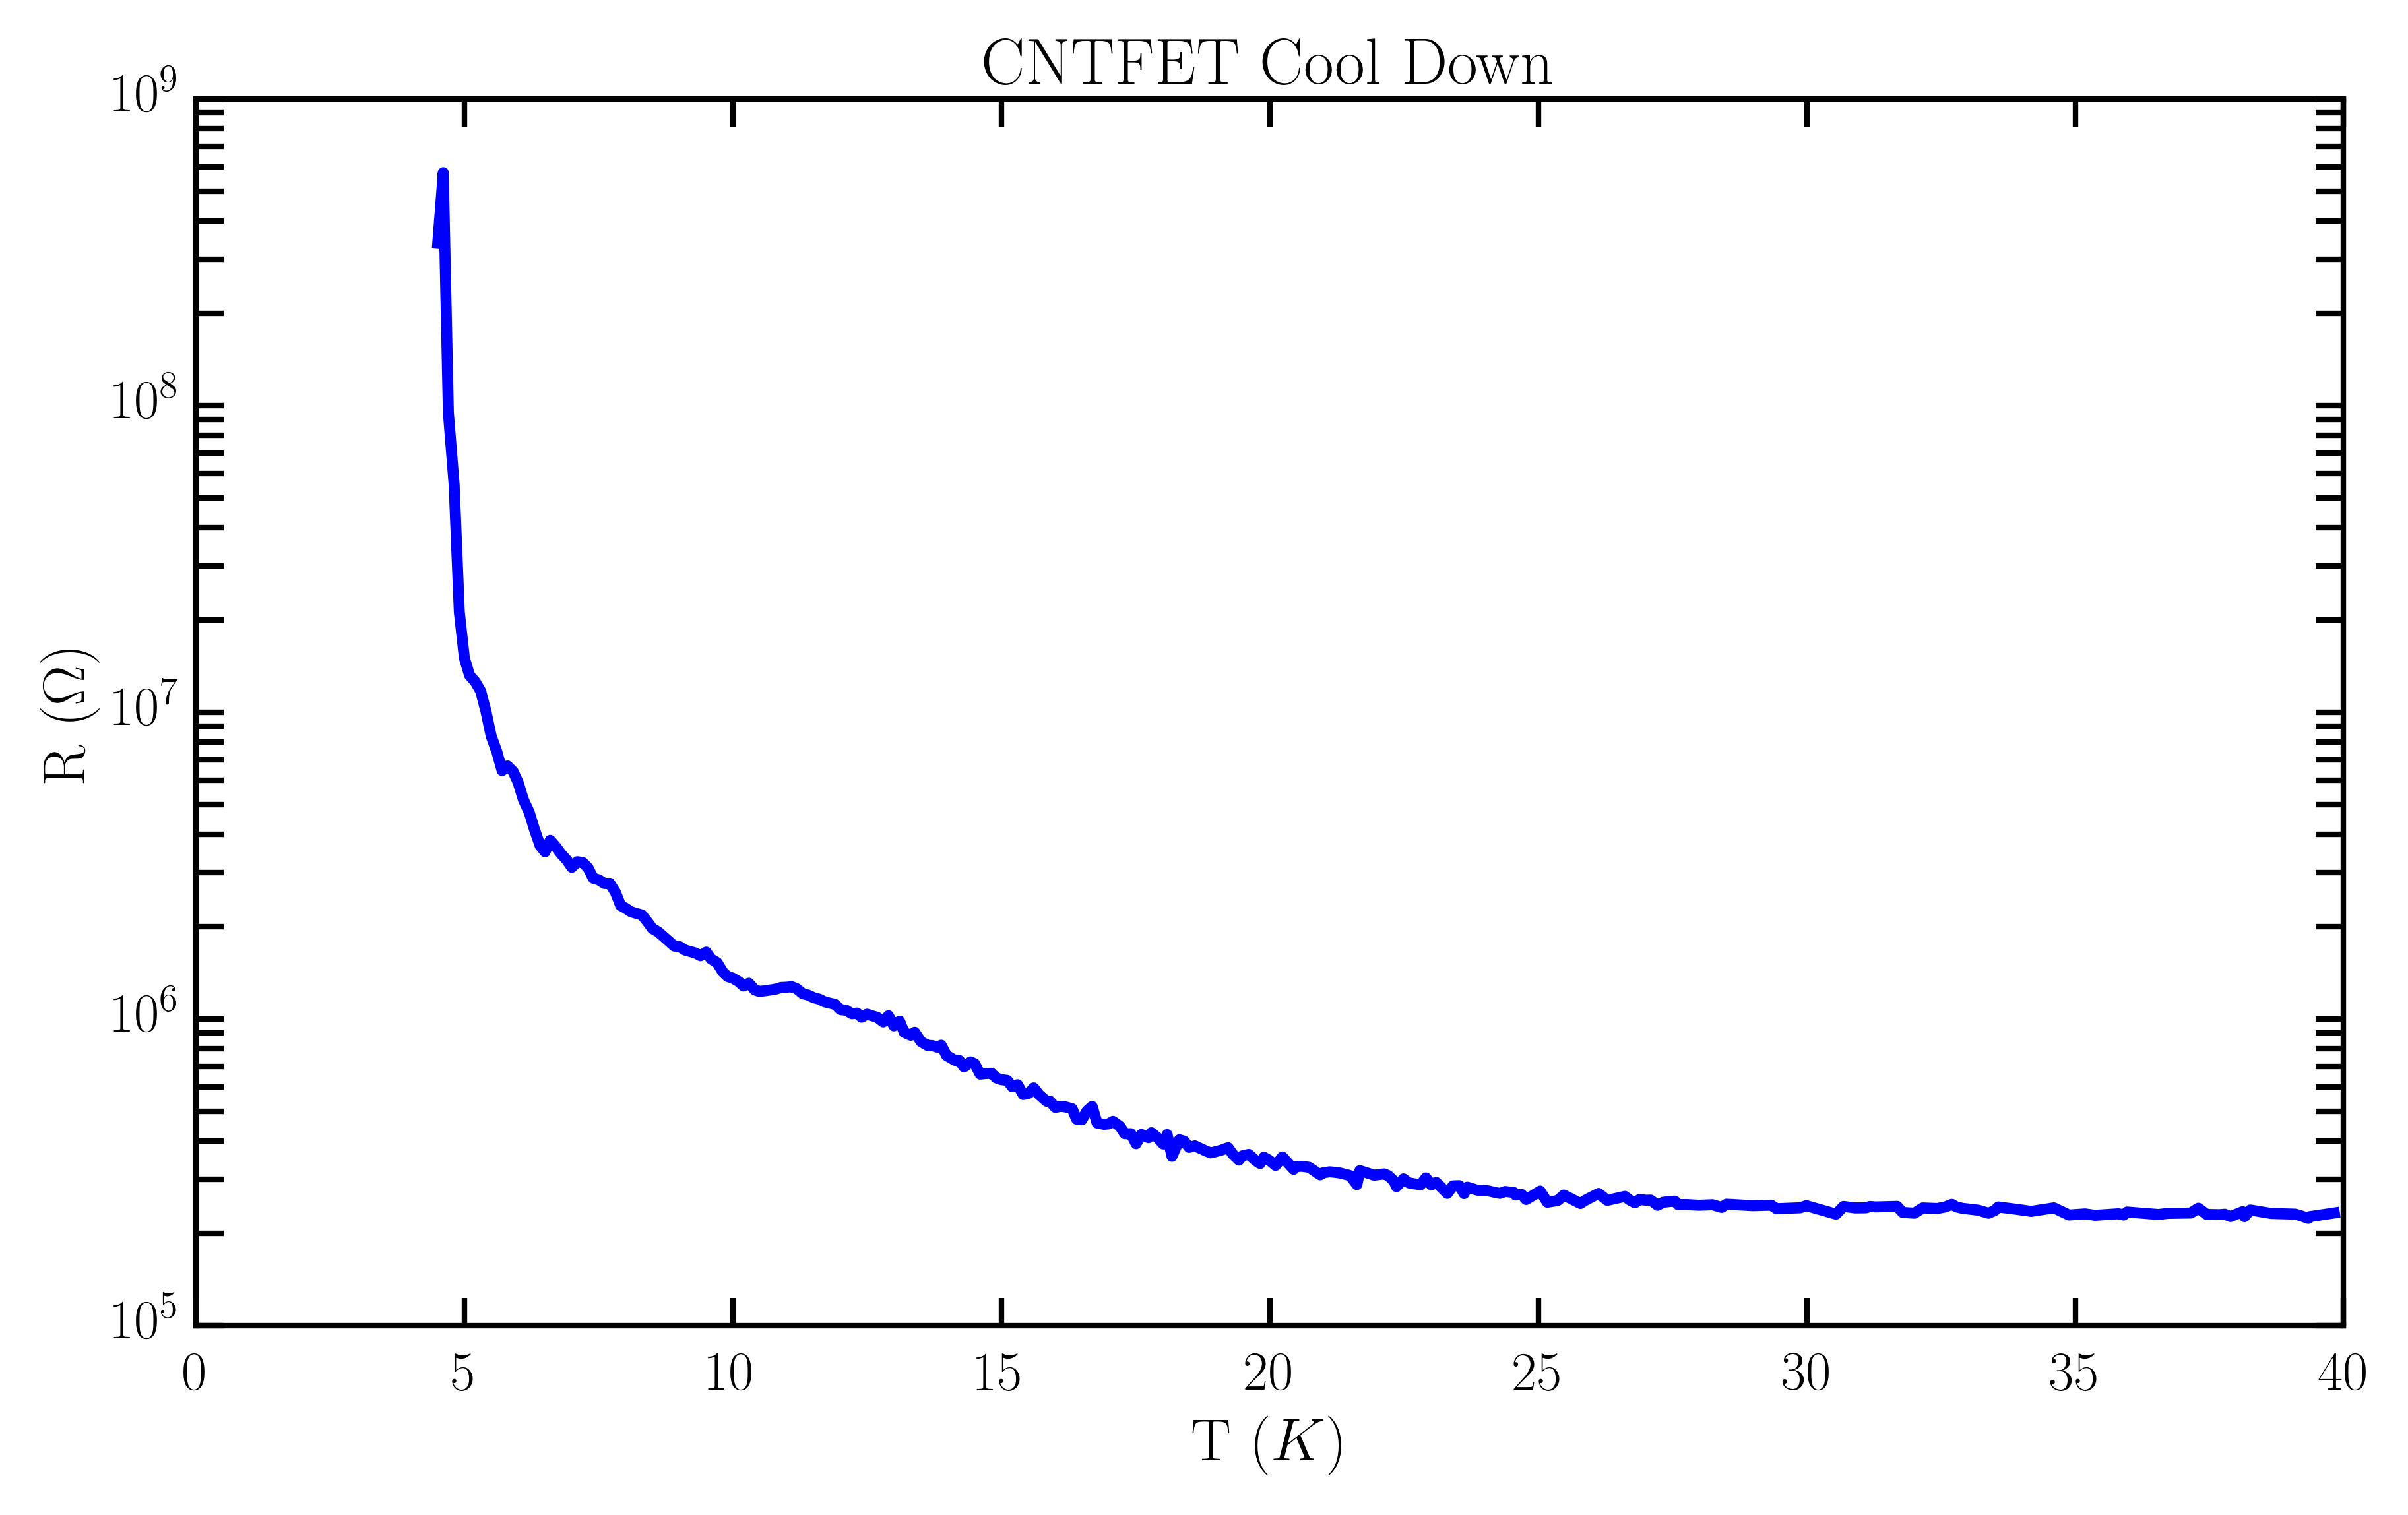
\includegraphics[width=0.6\textwidth]{chapter2/cntfet_cooldown.png}
    \caption{R-T curve of a CNTFET cooled to \SI{4}{\kelvin}}
    \label{fig:CNT_RT}
\end{figure}

Once the device is cold, the filling of electrons can be controlled by varying the bias and gate voltages. A schematic of the relevant energies is seen in Figure \ref{fig:QD_model}. The bias voltage can be used to change the relative chemical potential of the source and drain metals. The gate voltage is then used to change the chemical potential on the quantum dot relative to the source/drain.

\begin{figure}
    \centering
    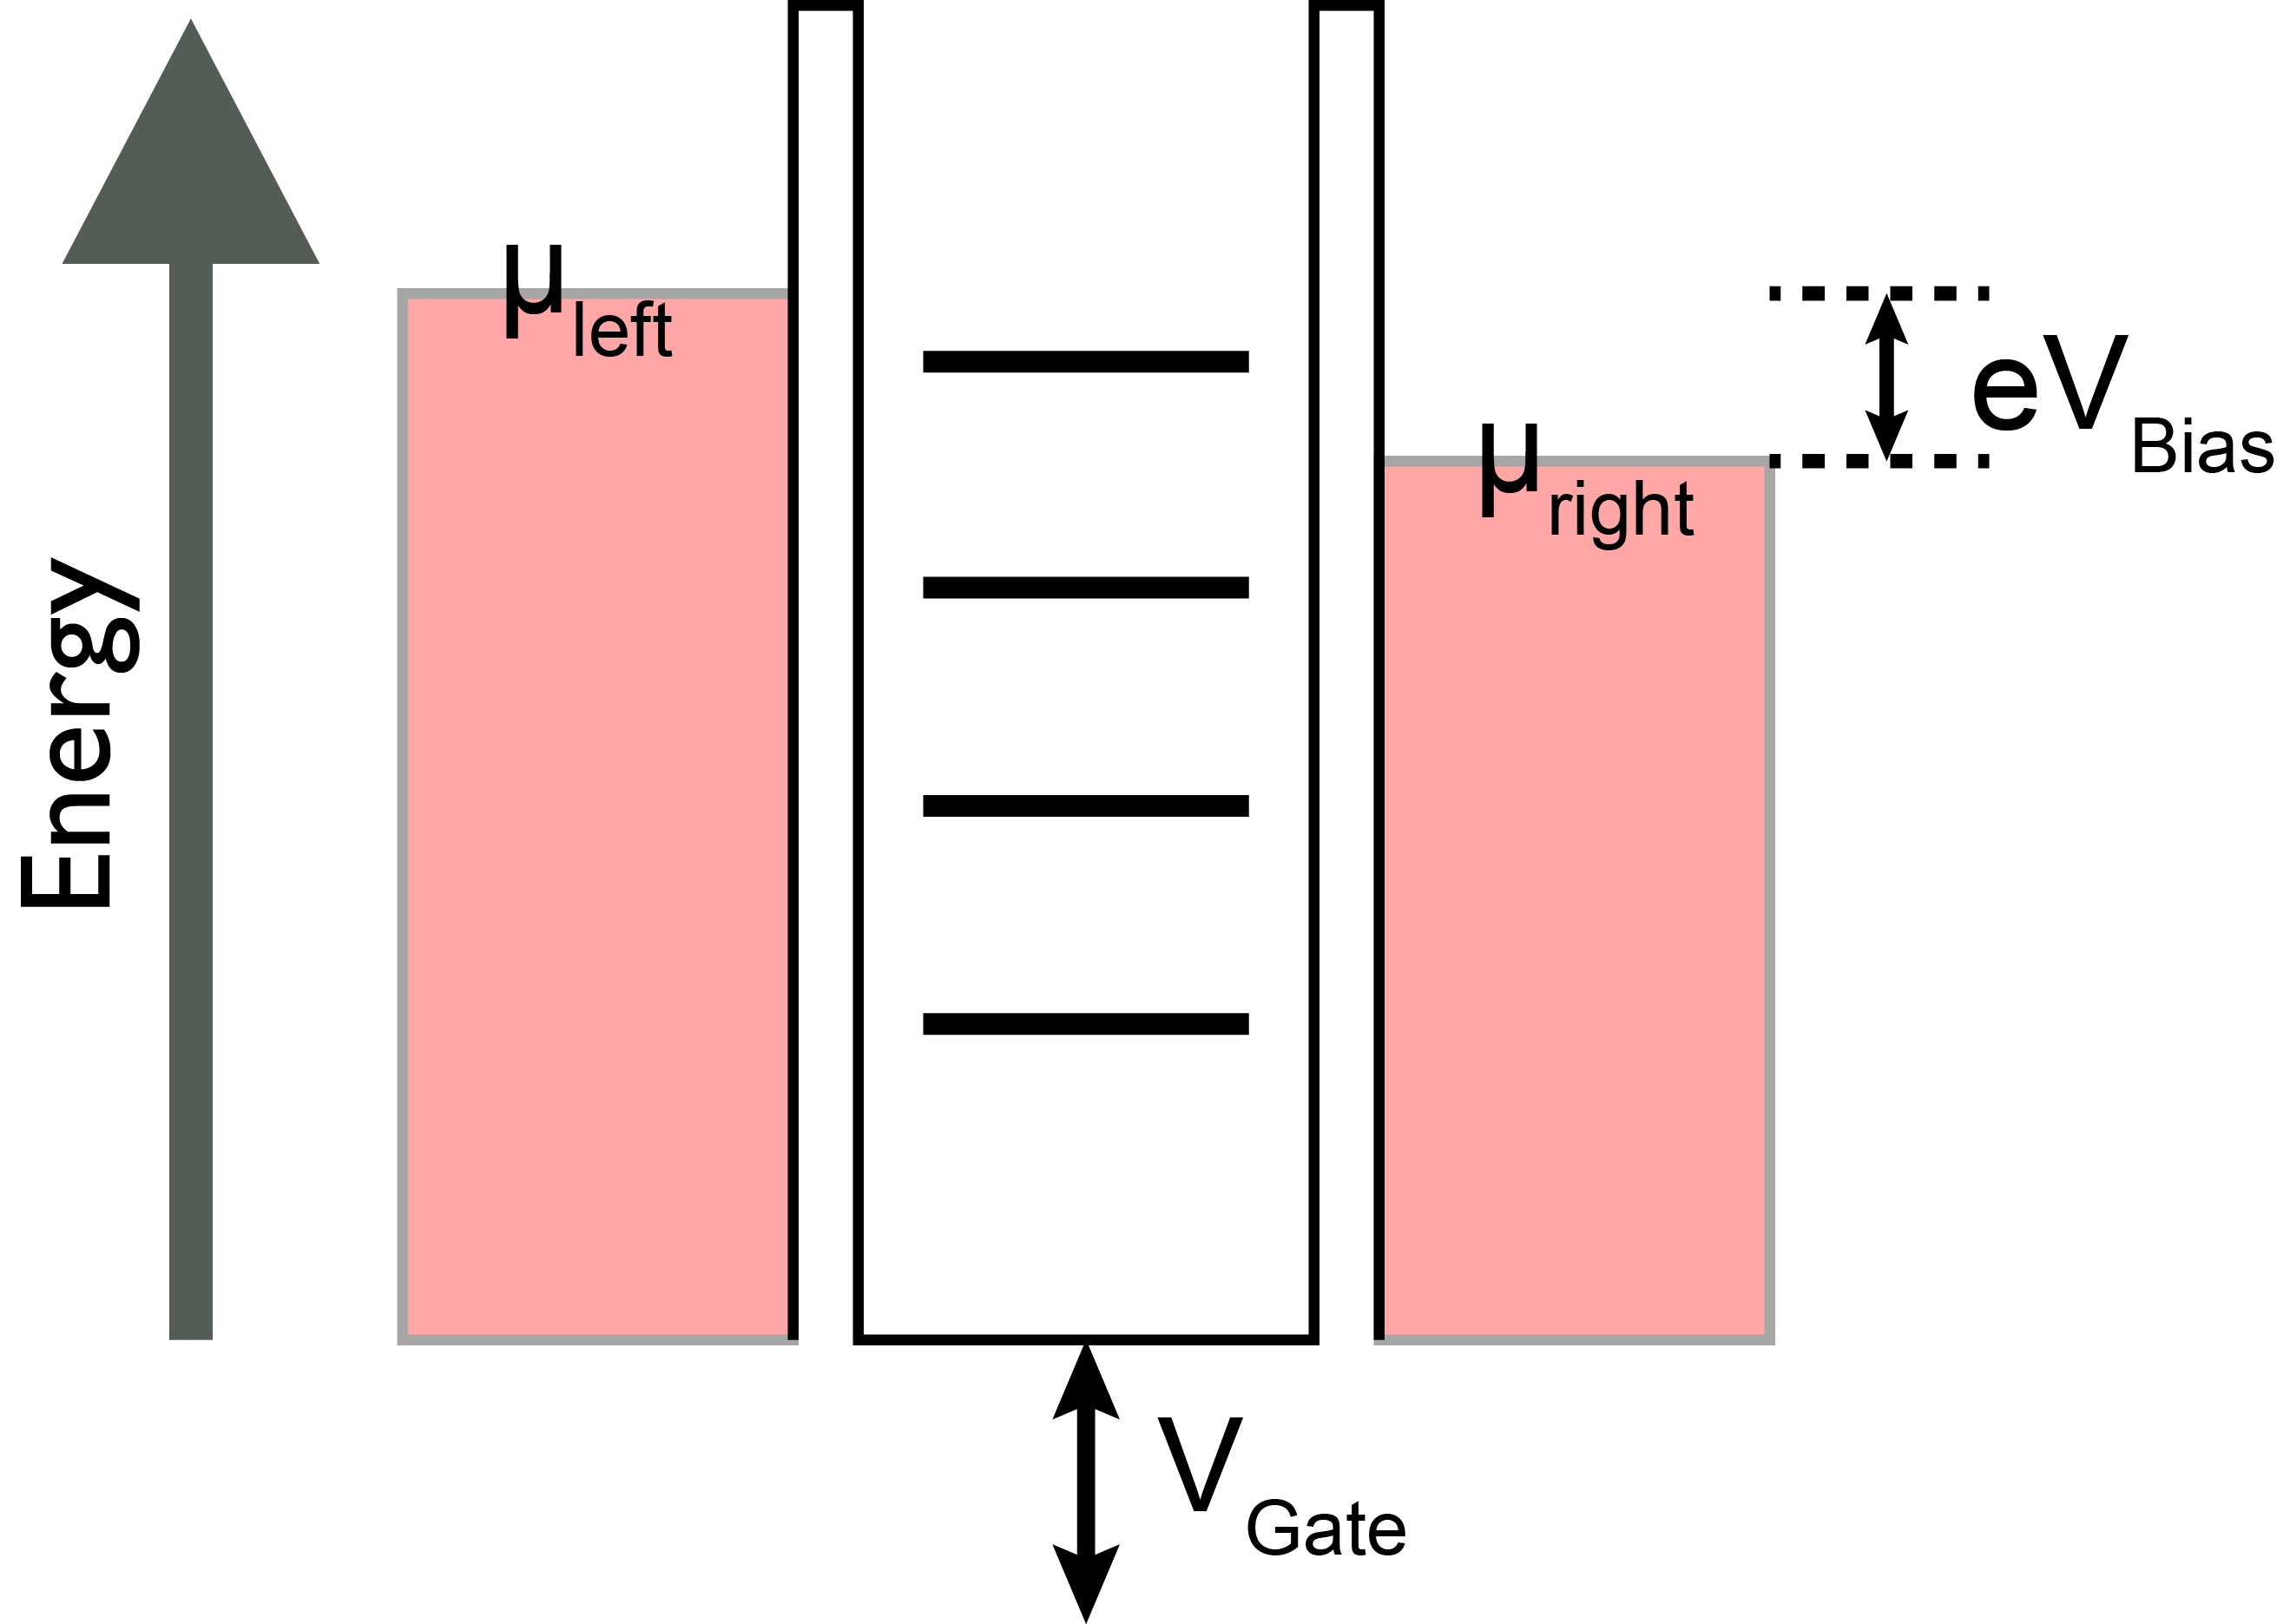
\includegraphics[width=0.5\textwidth]{chapter2/quantum_dot_model.png}
    \caption{Quantum dot energy diagram.}
    \label{fig:QD_model}
\end{figure}

The model we will use to discuss this device is called the constant interaction model. Tunnel barriers naturally form at the interface between the metal contacts and the nanotube. At low temperatures, this leads to weak tunneling on/off the nanotube (quantum dot). Because of this, the number of electrons confined on the dot at any given time is an integer, N. Adding an additional electron to the dot requires overcoming the Coulomb repulsion between the additional electron and those already confined on the dot. The constant interaction model treats this charging energy as a constant, regardless of the number of electrons confined on the dot. The model also assumes that the states on the quantum dot are not affected by the electron-electron interactions.

With these assumptions, it is simple to find the energy required to add an electron to the dot. To begin, the total energy on the dot can be approximated.

\begin{equation}
    U(N) = \frac{[e(N-N_0) - C_gV_g]^2}{2C} + \sum_{N}^{} E_n
\end{equation}

Here $N_0$ is the charge on the dot a zero gate voltage, $C_g$ is the gate capacitance, and $C = C_source + C_drain + C_gate$. The summation represents the sum over all of the filled quantum dot leves, denoted by $E_n$. The chemical potential is defined as $\mu(N) = U(N) - U(N+1)$. 

\begin{equation}
    \mu(N) = (N - N_0 - \frac{1}{2})\frac{e^2}{2C} - \frac{eC_gV_g}{C} + E_N
\end{equation}

Finally, the addition energy is given by the change in chemical potential from the $N$ to $N+1$ levels.

\begin{align}
    \Delta \mu(N) &= \frac{e^2}{2C} + (E_N+1 - E_N) \nonumber \\
    \Delta \mu(N) &= \frac{e^2}{2C} + \Delta E  \label{eq:addition_energy}
\end{align}

Equation \ref{eq:addition_energy} gives the amount of energy required to add the Nth electron to the quantum dot. Note that the first term in this energy is the constant interaction term representing the Coulomb repulsion, $E_{charging} = \frac{e^2}{2C}$. 

The simplest measurement to make on a quantum dot like the one described here, is to measure the conductance as a function of the gate voltage. Figure \ref{fig:gate_blockade} shows diagrammatically how the process works. At very small bias ($\mu_{left} \sim \mu_{right}$), the gate voltage is varied. When the chemical potential on the source/drain are resonant with a level on the quantum dot, a peak is observed in the conductance. Otherwise, conductance  across the dot is suppressed. Spacing between conductance peaks should follow Equation \ref{eq:addition_energy}.

\begin{figure}
    \centering
    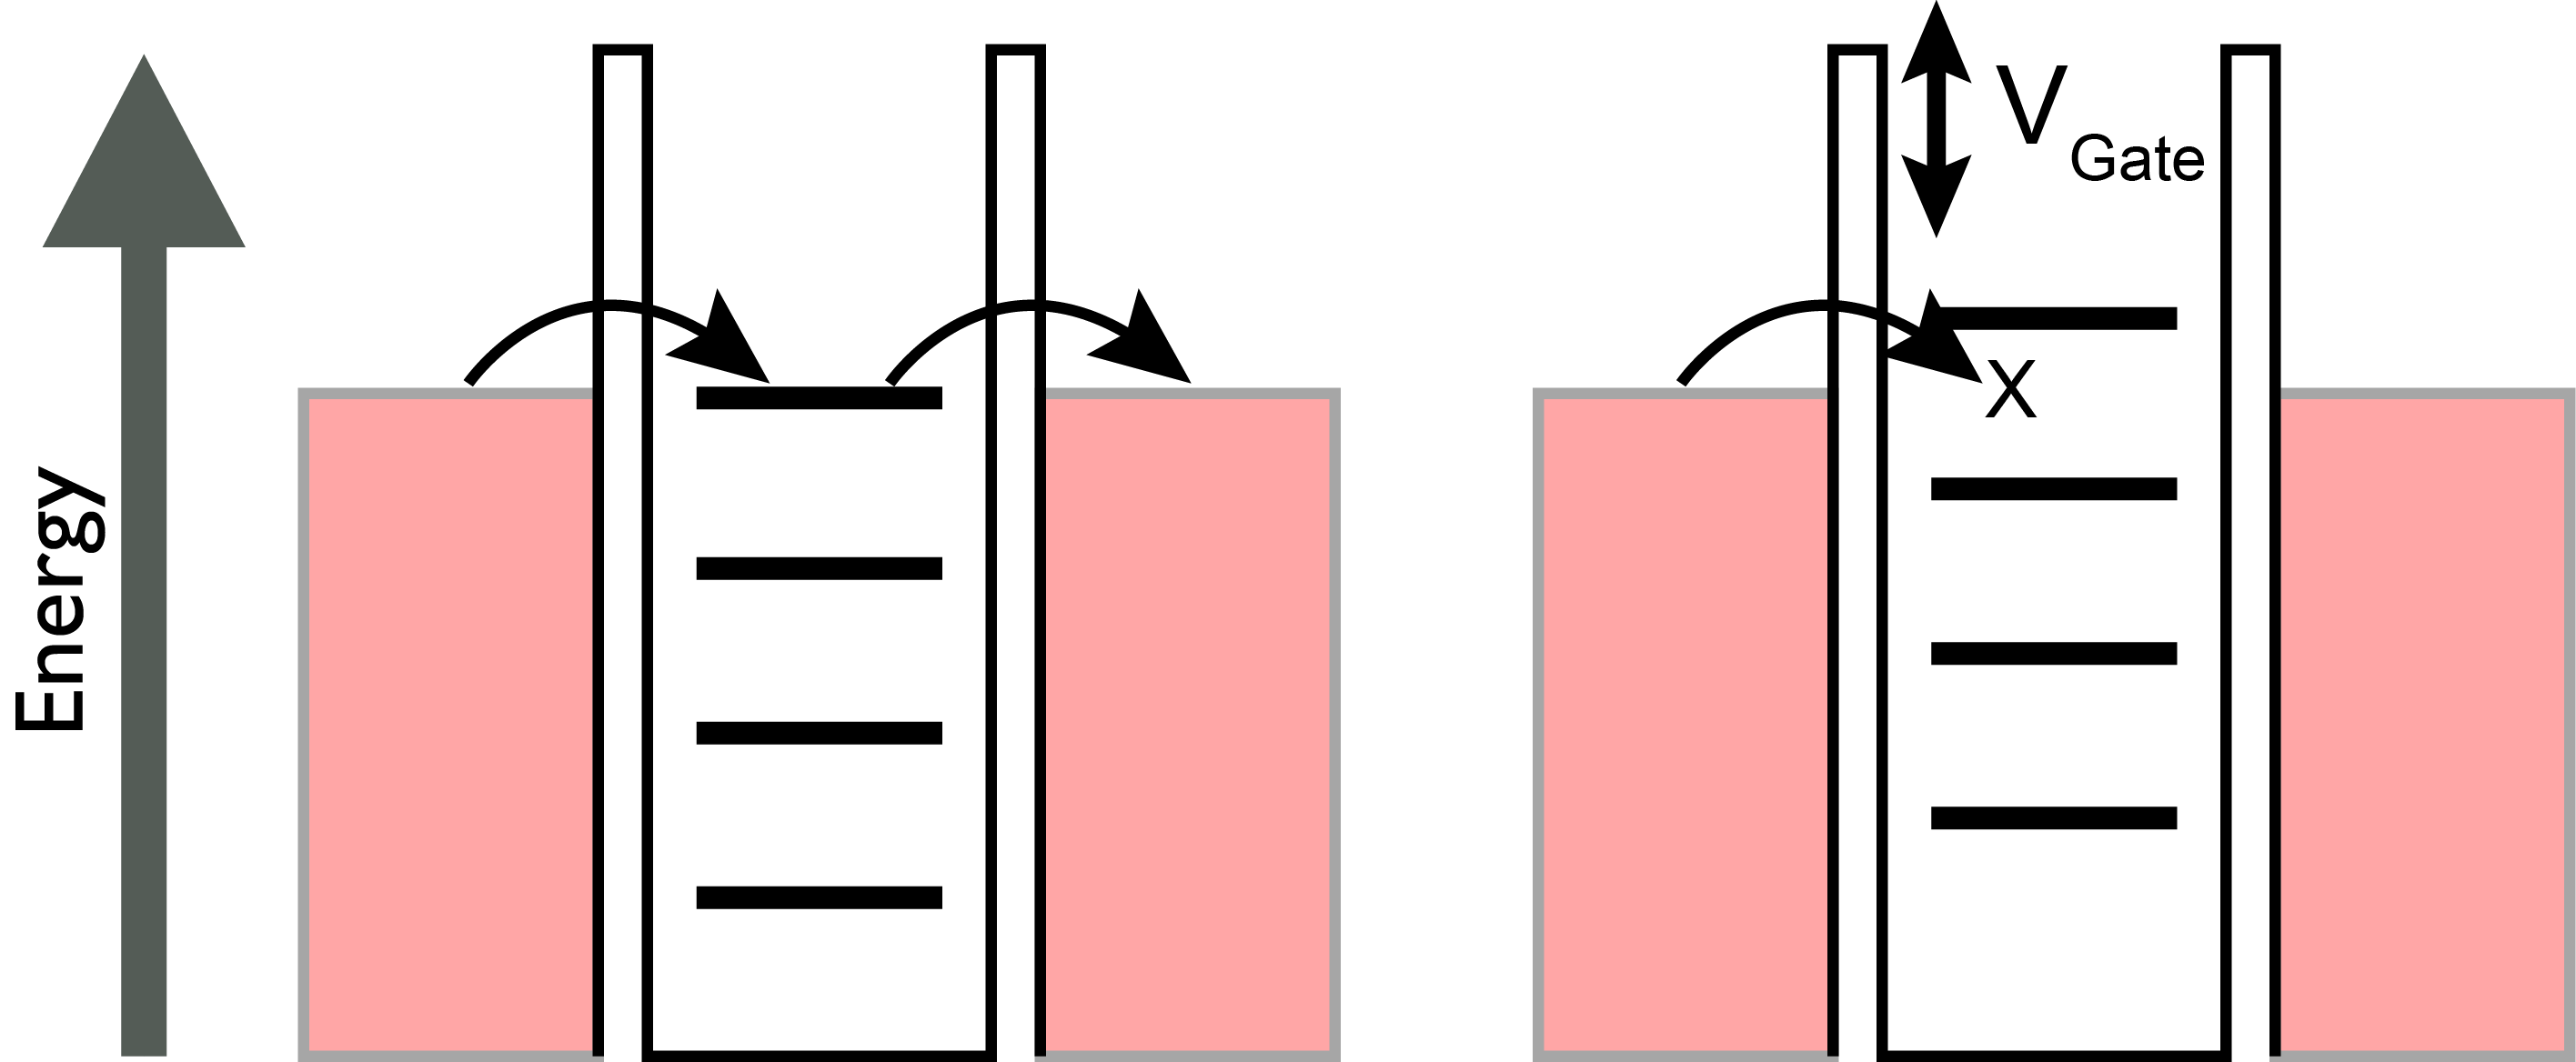
\includegraphics[width=0.8\textwidth]{chapter2/gate_blockade.png}
    \caption{Left: A quantum dot level resonant with the source/drain chemical potential. Right: The same device in the blockaded region.}
    \label{fig:gate_blockade}
\end{figure}

Figure \ref{fig:real_gate} shows conductance as a function of gate voltage through an actual carbon nanotube quantum dot device. A close look at the spacing of the conductance peaks reveals some hints of four-fold symmetry that is an important part of the structure of the nanotube quantum dot. Adding the first electron to the dot costs an energy $ \Delta \mu(N) = \frac{e^2}{2C} + \Delta E$. However, the electron spin and valley degeneracy combine to give each level in the quantum potential well a degeneracy of four. The next three electrons added move into the same level, which only requires an energy of $\Delta \mu(N) = \frac{e^2}{2C}$ for each electron. This pattern continues for each level on the dot, such that the energy required to add the $N$ electron is always larger than the energy required to add the $N+1$, $N+2$, and $N+3$ electrons.

\begin{figure}
    \centering
    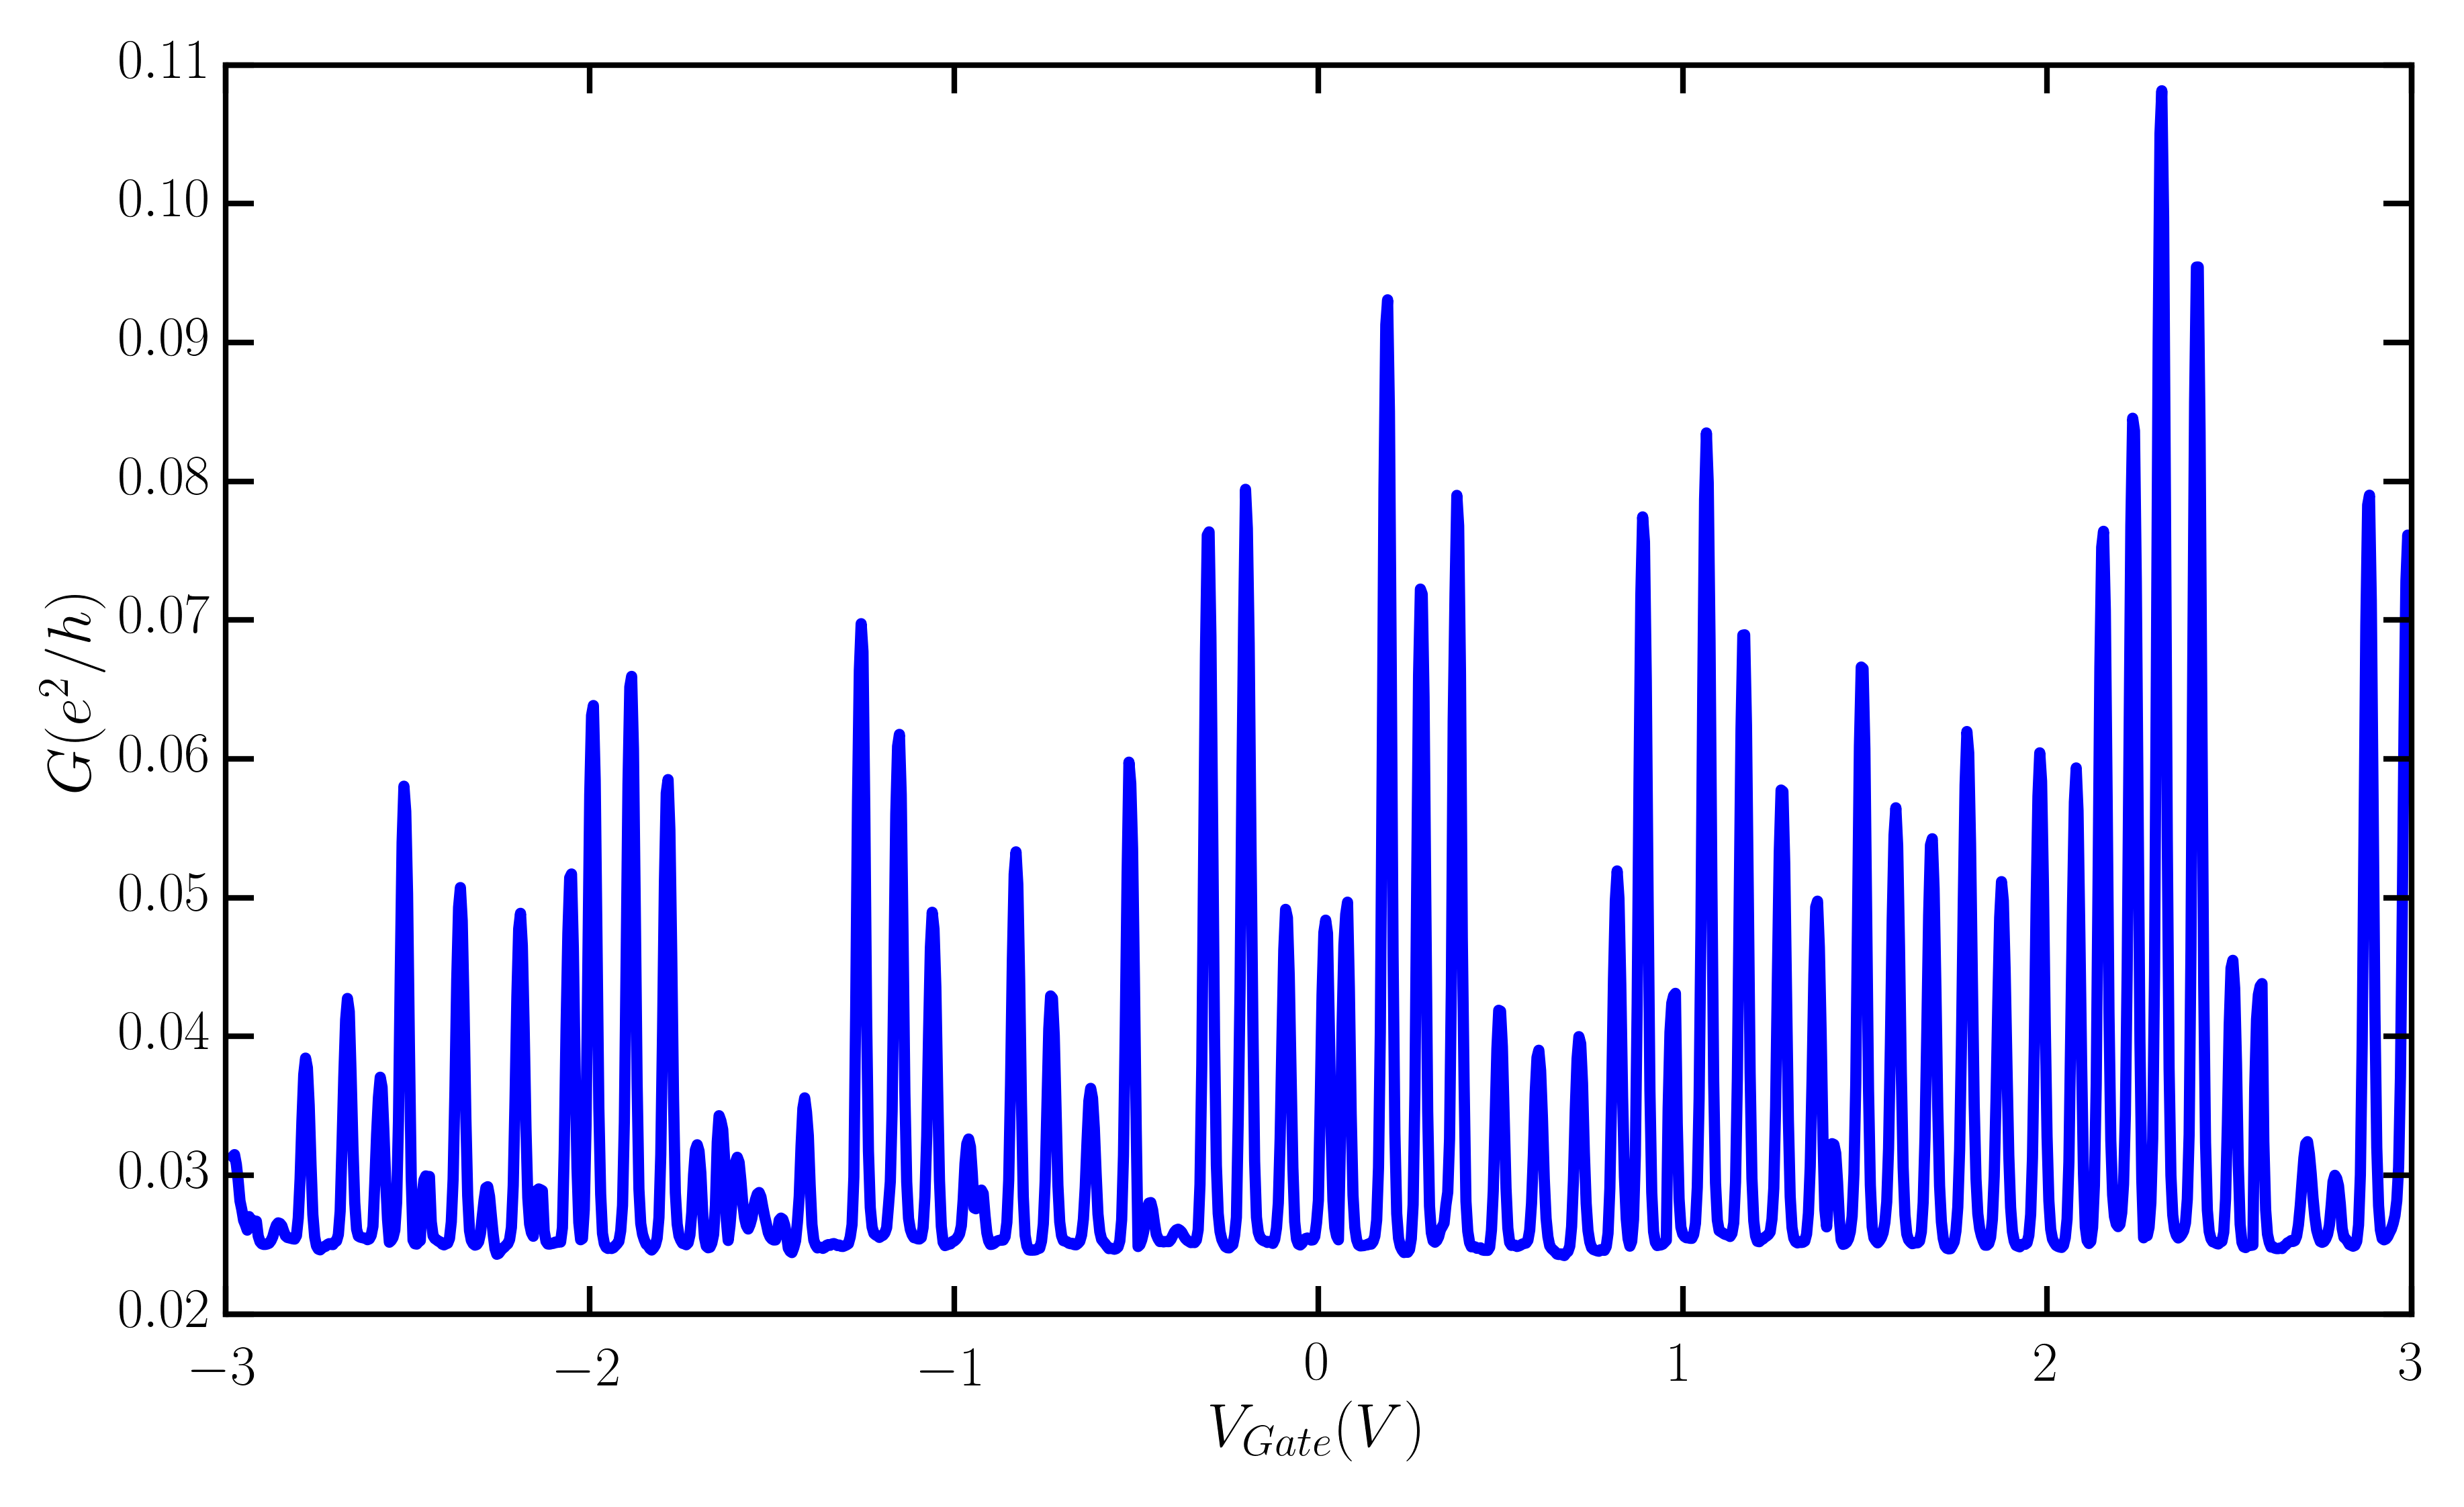
\includegraphics[width=0.8\textwidth]{chapter2/gate_sweep.pdf}
    \caption{Conductance as a function of applied gate voltage in a cobalt contacted nanotube quantum dot. Inset: A close up showing a region with clear 4 fold symmetry.}
    \label{fig:real_gate}
\end{figure}

Varying the bias voltage also changes the relative alignment of the energy levels on the dot and the chemical potentials of the source and drain electrodes,, as illustrated in Figure \ref{fig:bias_blockade}. If a level on the quantum dot lies between the chemical potentials of the source and the drain (the bias window), conductance is possible. Otherwise, if there are no energy levels in the bias window, the conductance through the device is suppressed. With further increases of the bias voltage, higher order conductance processes are possible. 

\begin{figure}
    \centering
    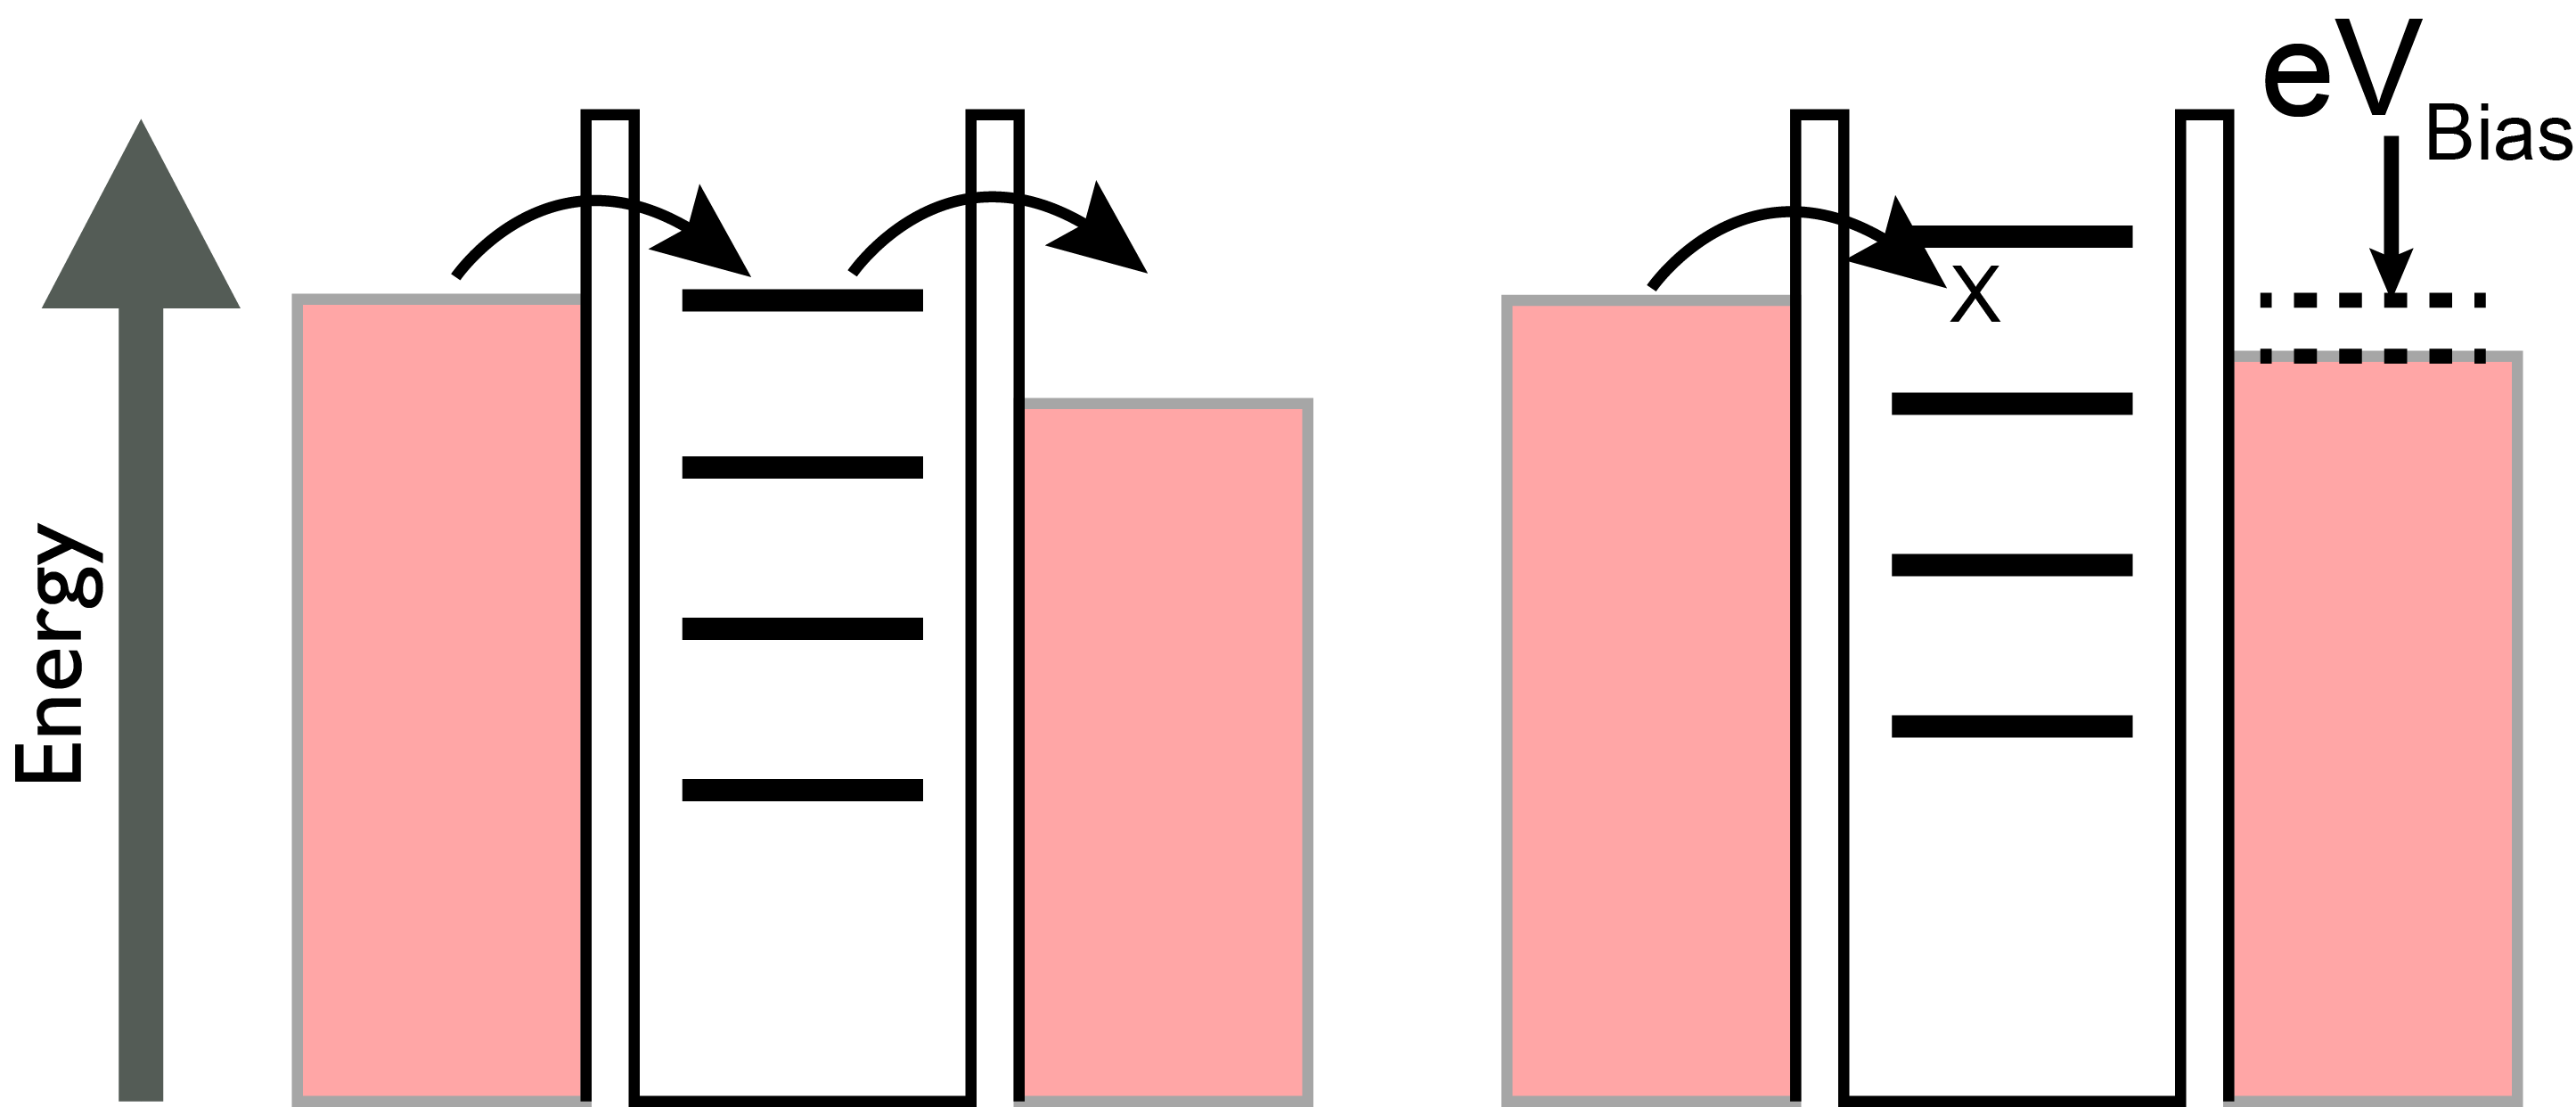
\includegraphics[width=0.8\textwidth]{chapter2/bias_blockade.png}
    \caption{Left: A quantum dot level resonant with the drain chemical potential. Right: The same device in the blockaded region.}
    \label{fig:bias_blockade}
\end{figure}

\begin{figure}
    \centering
    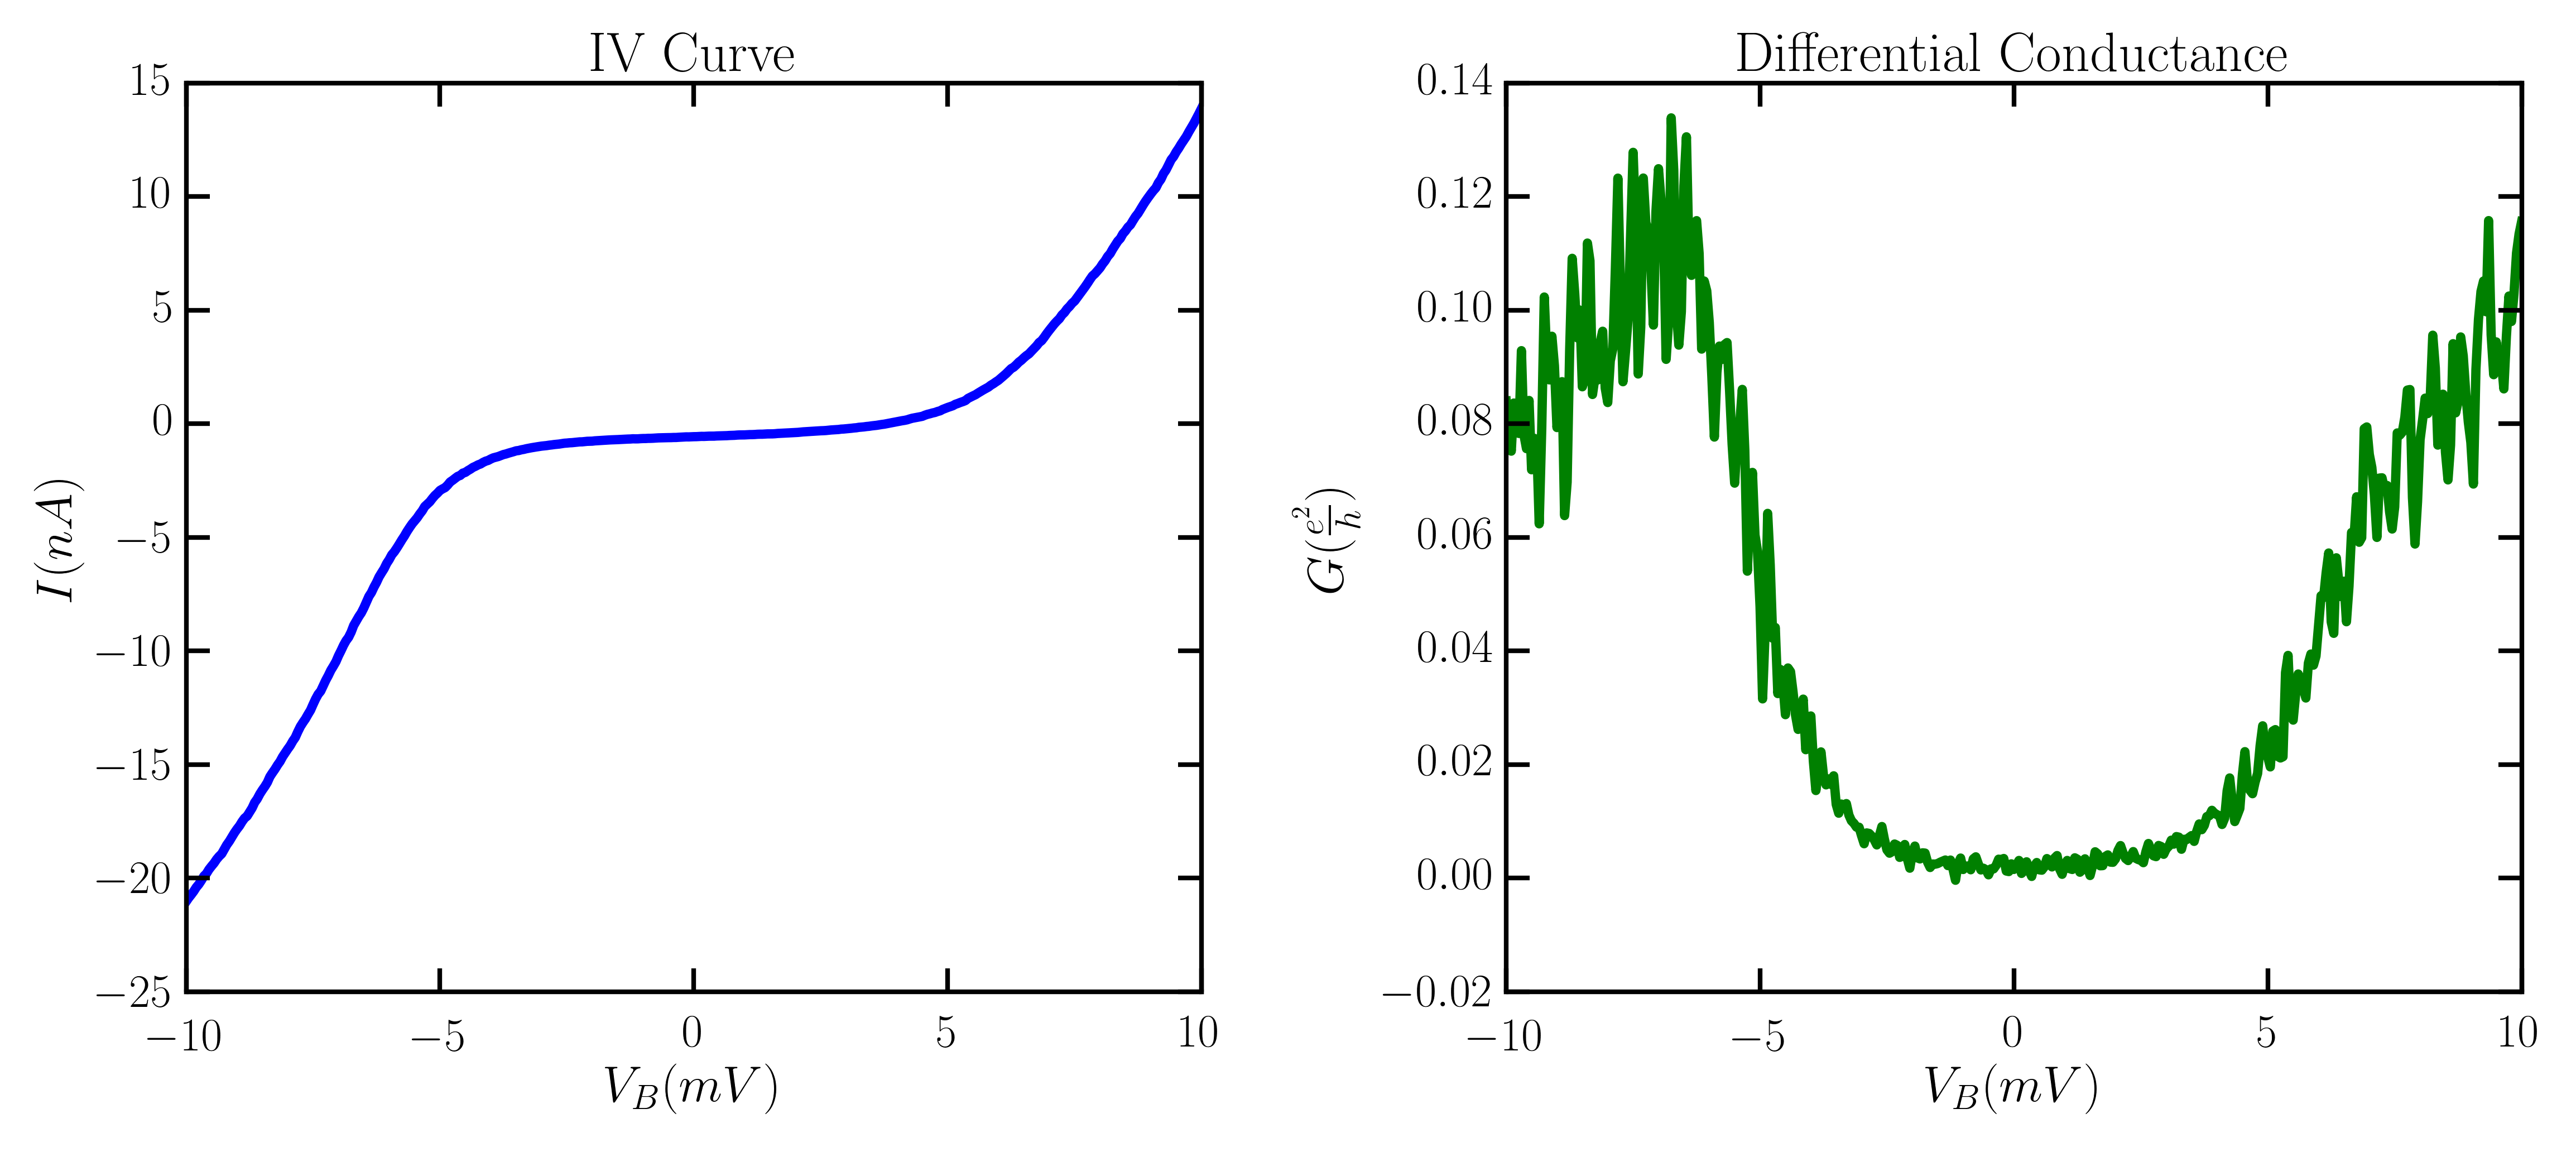
\includegraphics[width=0.8\textwidth]{chapter2/bias_sweep.png}
    \caption{Left: An IV curve at fixed gate voltage Right: Differential conductance measured at fixed gate voltage.}
    \label{fig:real_bias}
\end{figure}

Figure \ref{fig:real_bias} shows current and conductance as a function of applied bias voltage in the blockaded regime. The differential conductance is suppressed across the dot at low bias voltage. At higher bias, the bias window increases, eventually encompassing an energy level on the dot, which causes the conductance to increase. A further increase of the bias voltage allows for transport through excited states and higher order processes, which will be discussed in later chapters.

Finally, measuring conductance as a function of both the bias and gate produces a stability diagram of the quantum dot. An example of this can be seen in Figure \ref{fig:coulomb_diamonds}. Looking at a cut of this plot at constant bias reproduces Figure \ref{fig:real_gate}. Similarly, a cut at constant gate voltage reproduces Figure \ref{fig:real_bias}. Putting both together produces diamond-shaped regions in which the charge on the quantum dot in constant, denoted by $N-1$, $N$, and $N+1$ in the figure. The white dashed lines serve as a guide to the eye. The two black arrows mark the level spacing, $\Delta E$, and addition energy $E_{Add}$ (or $\Delta \mu$). By measuring both of these quantities it is possible to know the level spacing on the quantum dot and the capacitance of the device. By observing changes in the conductance peaks at different fillings and applied fields, much can be learned about the energy levels, interactions, and transport across the quantum dot.

\begin{figure}
    \centering
    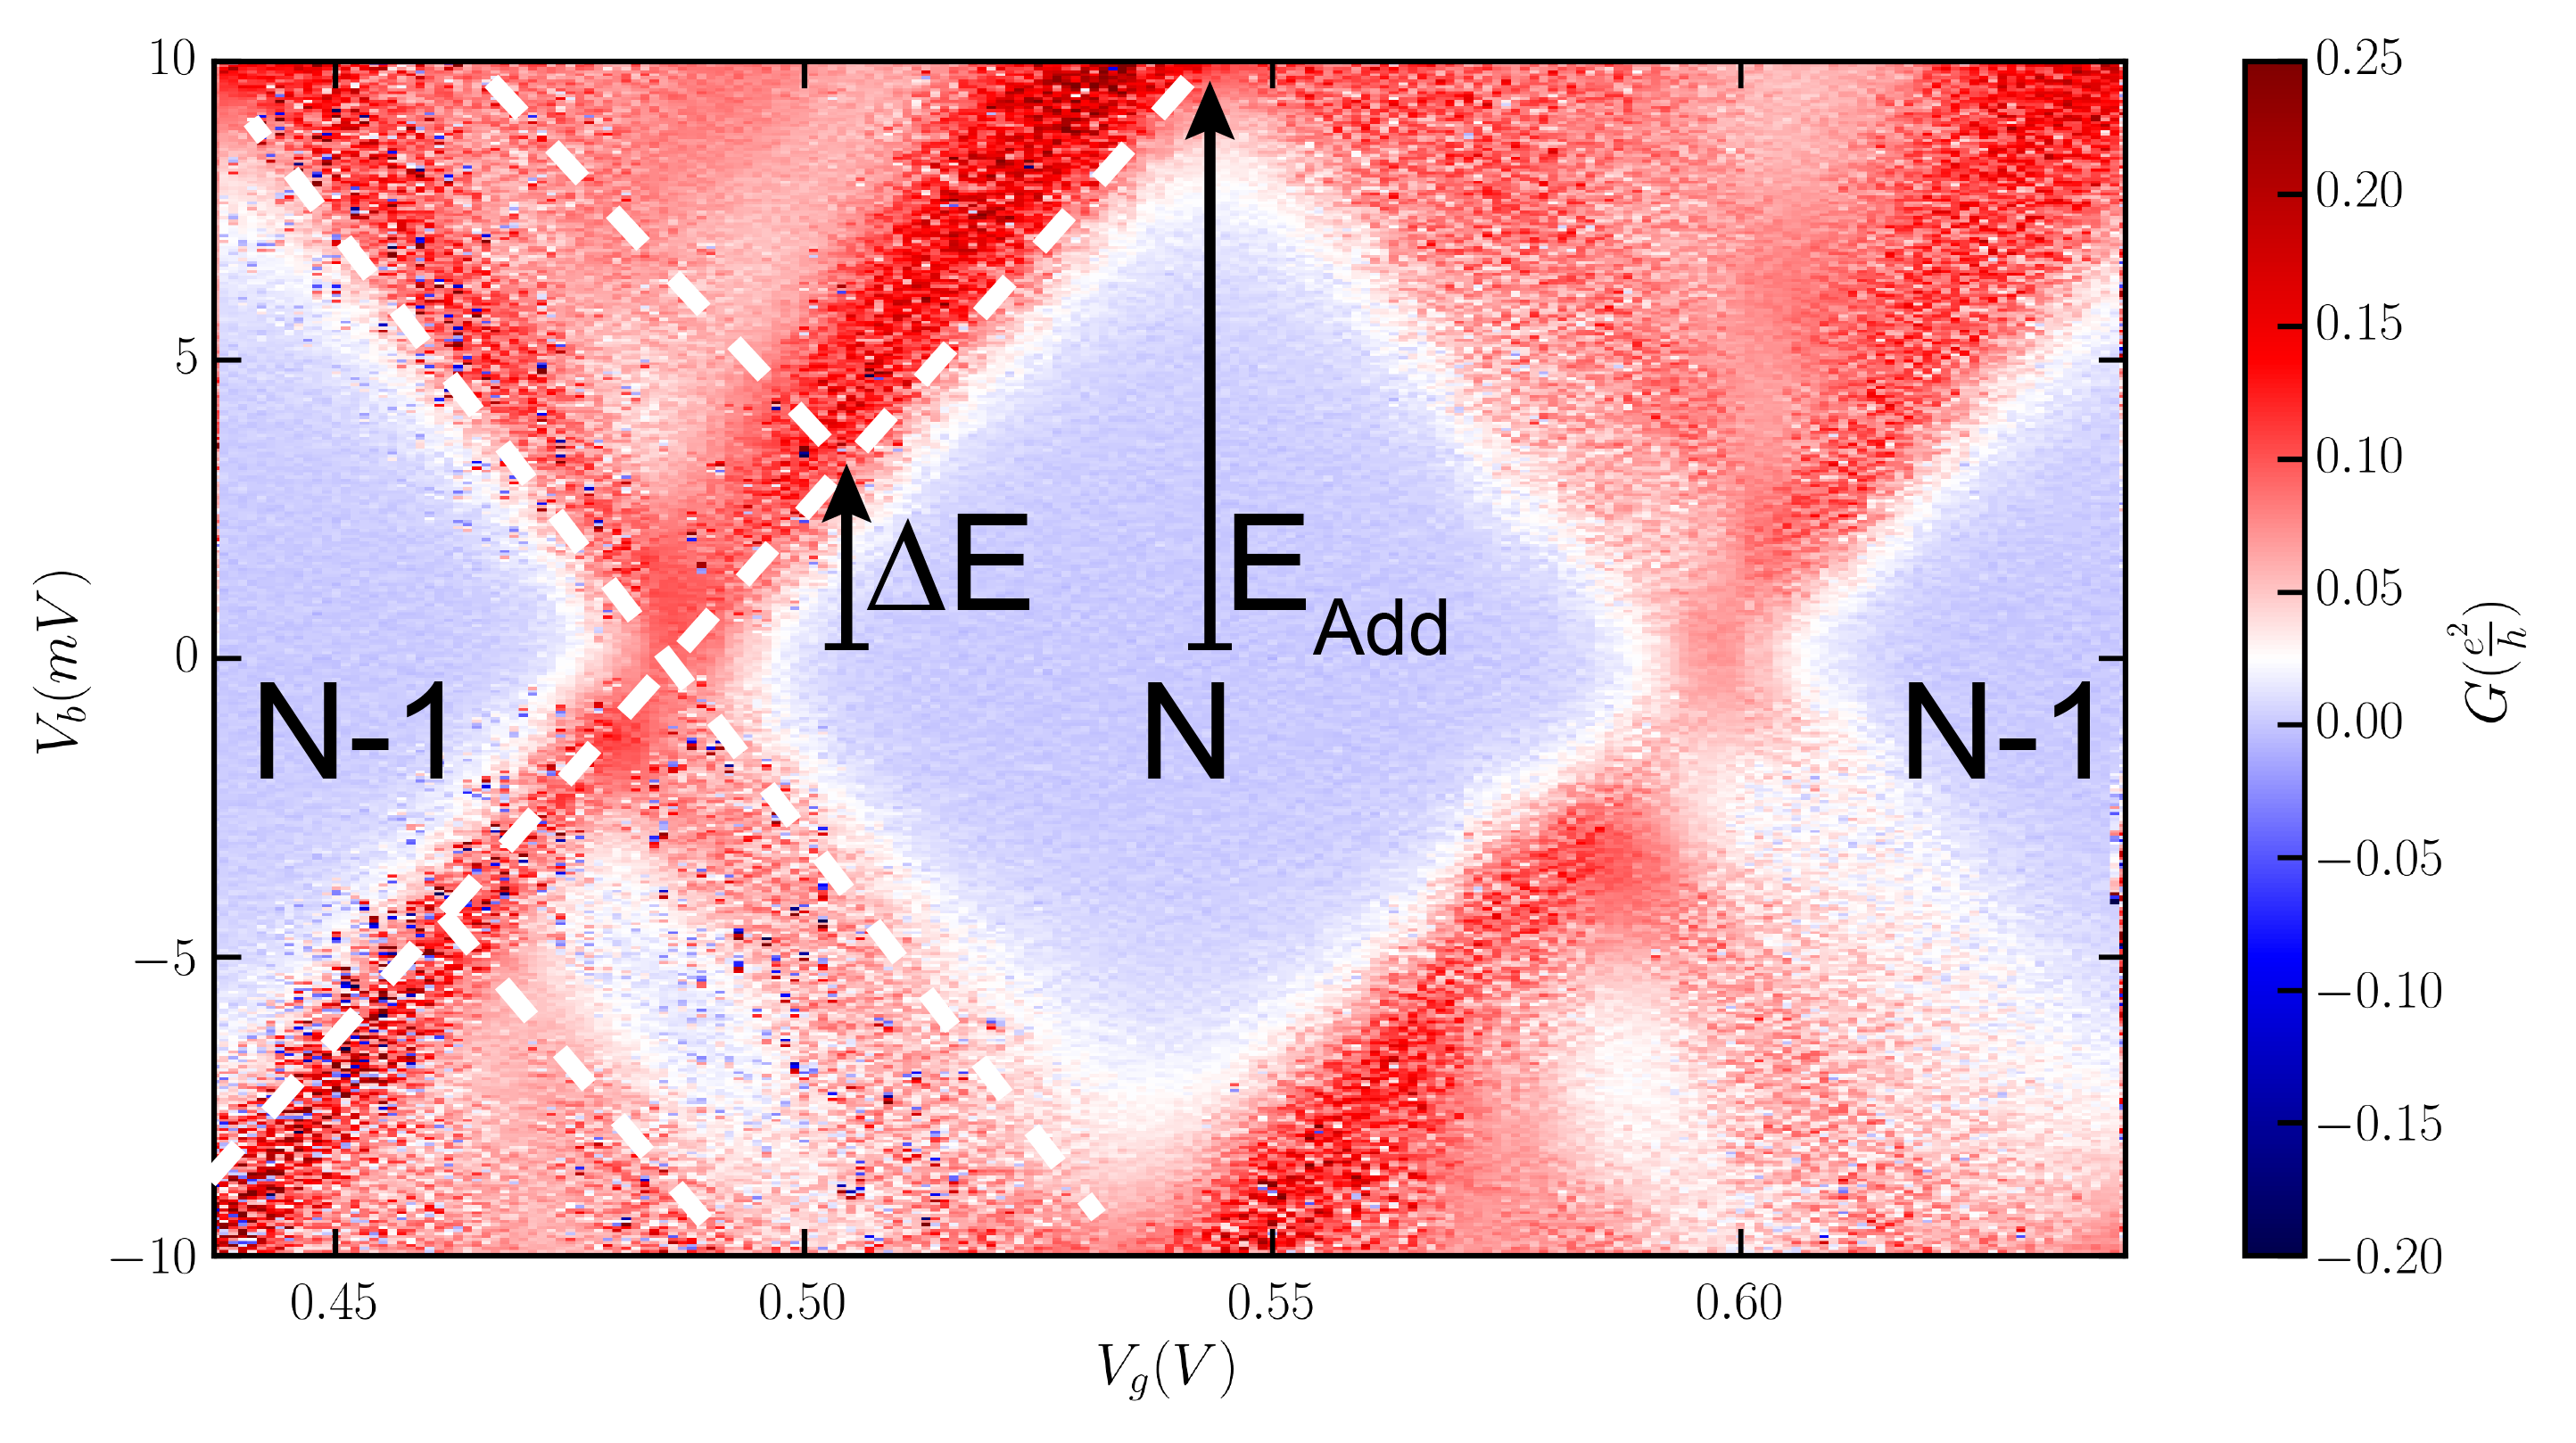
\includegraphics[width=0.7\textwidth]{chapter2/diamond_diagram.pdf}
    \caption{Conductance of a cobalt contacted nanotube quantum dot at 4K as a function of bias and gate voltages.}
    \label{fig:coulomb_diamonds}
\end{figure}

As an illustrative example the properties of the device measured in Figure \ref{fig:coulomb_diamonds} can be calculated. Here the level spacing on the dot is measured to be $\Delta E = 4meV$ and the addition energy $E_{Add} = 9meV$. At low energies the dispersion relation of the nanotube can be assumed to be roughly linear $\varepsilon(k) = \hbar v_f k$. $k$ is quantized because of the confinement potential created by the leads $k = \frac{n\pi}{L}$. The level splitting can then be written as $\Delta E = \frac{\hbar v_f \pi}{L}$. Using the measured value of $\Delta E$ gives an estimate of $L = 520nm$, which is consistent with the device design of \SI{500}{\nano\meter}. This result can now be used, along with the addition energy, to find the total capacitance of the quantum dot. Starting with $E_{Add} = \frac{e^2}{2C} + \Delta E$ gives an estimate of $C=10^{-17}F$, which is consistent with typical carbon nanotube quantum dot measurements. % derivation of CNT band structure, explanation of QD + measurements
%% all about growing, placing, imaging, filtering carbon nanotubes

\chapter{Carbon Nanotube Growth and Placement}
\label{sec:growth}
\chaptermark{Growth and Placement}

In the years since their discovery, many methods of producing electronic devices from carbon nanotubes have been developed. These include random dispersion (Section \ref{sec:random_dispersion}), on-substrate catalyst island growth (Section \label{sec:catalyst_island}) and stamping \cite{Wu2010, Pei2012}. For this work, the first two methods were successfully used to produce carbon nanotube quantum dots. It was found that the catalyst island growth was much easier to implement and required much less processing time per device.

\section{Random Dispersion}
\label{sec:random_dispersion}

The first successful method of nanotube device fabrication was what will be referred to here as random dispersion. First, nanotubes are grown in bulk through chemical vapor deposition (or other preferred method). Then, the nanotubes are suspended in a solution. Finally, the nanotubes are cast onto a substrate. Nanotubes can then be located relative to some predefined markers on the substrate.

\subsection{Catalyst}
\label{subsec:disperse_catalyst}

All of the devices discussed in this thesis have utilized the same, iron-based catalyst \cite{Kong1998, Kong1998a}. The simplest way to create this catalyst is to combine the ingredients in Table \ref{table:powder_catalyst} in a mortar and pestle and grind until it turns a uniform dark orange color. Adding some additional alumina seems to promote growth of longer tubes, possibly by lowering the density of tubes grown from each alumina/iron/molybdenum particle.

\begin{table}
	\centering
	\caption{Powder Catalyst}
    \begin{tabular}{ c | c }
    	\hline
        \ce{Fe(NO3)3*9H2O} & \SI{20}{\milli\gram} \\ \hline
        \ce{MoO2(acac)2} & \SI{5}{\milli\gram} \\ \hline
        \ce{Al2O3} & \SI{15}{\milli\gram} \\ \hline
    \end{tabular}
    \label{table:powder_catalyst}
\end{table}

\subsection{Growth}
\label{subsubsec:powder_cvd}

Of the many possible techniques for nanotube growth, we choose chemical vapor deposition for its simple implementation. The process is carried out in a Lindberg Blue tube furnace using a 1 inch diameter quartz tube. The furnace, quartz tube, and exhaust filtering are seen in Figure~\ref{fig:furnace_setup}. This setup has been repeatedly, and successfully, leak checked. Oxygen leaks can be detrimental to the nanotube growth process by forming \ce{CO} and \ce{CO2} with any free carbon, and potentially causing a fiery reaction with free hydrogen from the methane decomposition.

\begin{figure}
    \centering
    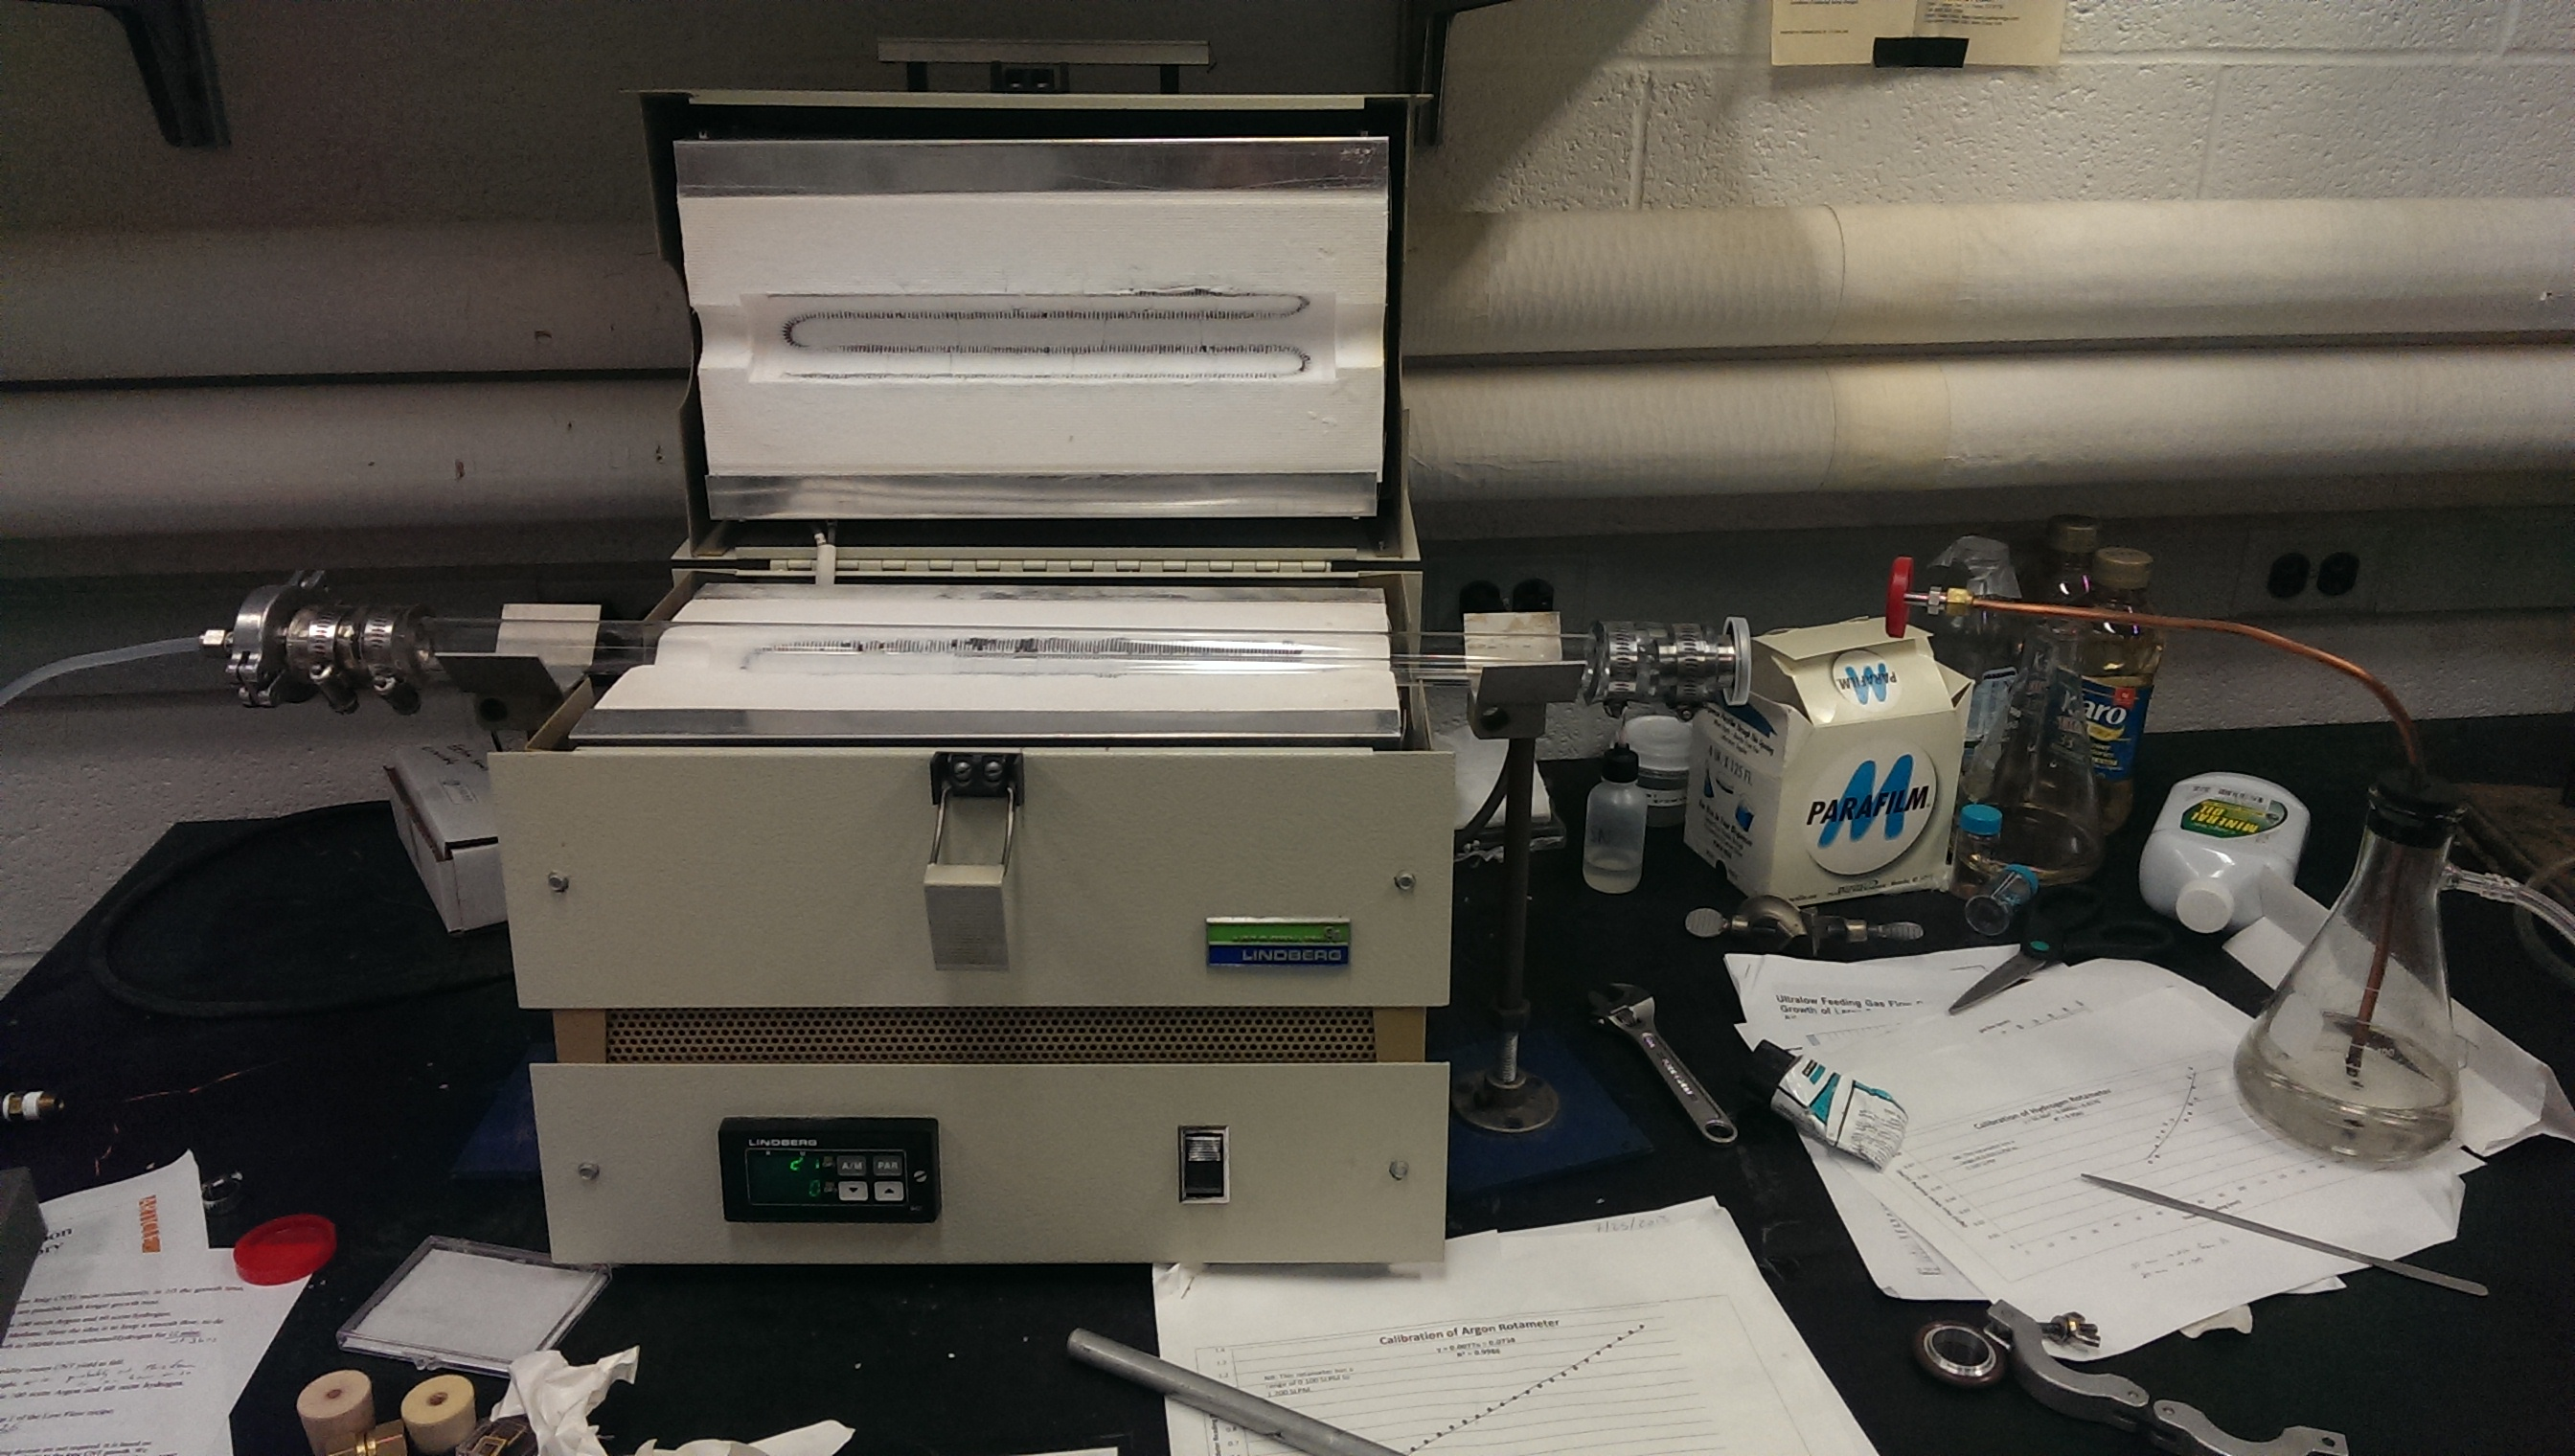
\includegraphics[width = 0.8\textwidth]{chapter3/furnace_setup.jpg}
    \caption{The tube furnace fitted with a 1" diameter quartz tube. The tube is sealed at both ends using 1" rubber tubing, cable clamps, and KF25 fittings. Gas flows from left to right in the picture. The gas flows out of the furnace into a mineral oil bubbler to keep hot hydrogen from reaching the air in the room. Gas then flows from the bubbler into the building exhaust.}
    \label{fig:furnace_setup}
\end{figure}

The gases used in the CVD process, argon, hydrogen, and methane, are fed into the furnace using a custom-made gas handling panel. The panel has three gas channels, each with its own analog flowmeter, needle valve, and on/off valve. A digital flowmeter placed at the right side of the panel reads the total flow of combined gas exiting the panel to the furnace. The gas handling panel can be see in Figure~\ref{fig:gas_panel}

\begin{figure}
    \centering
    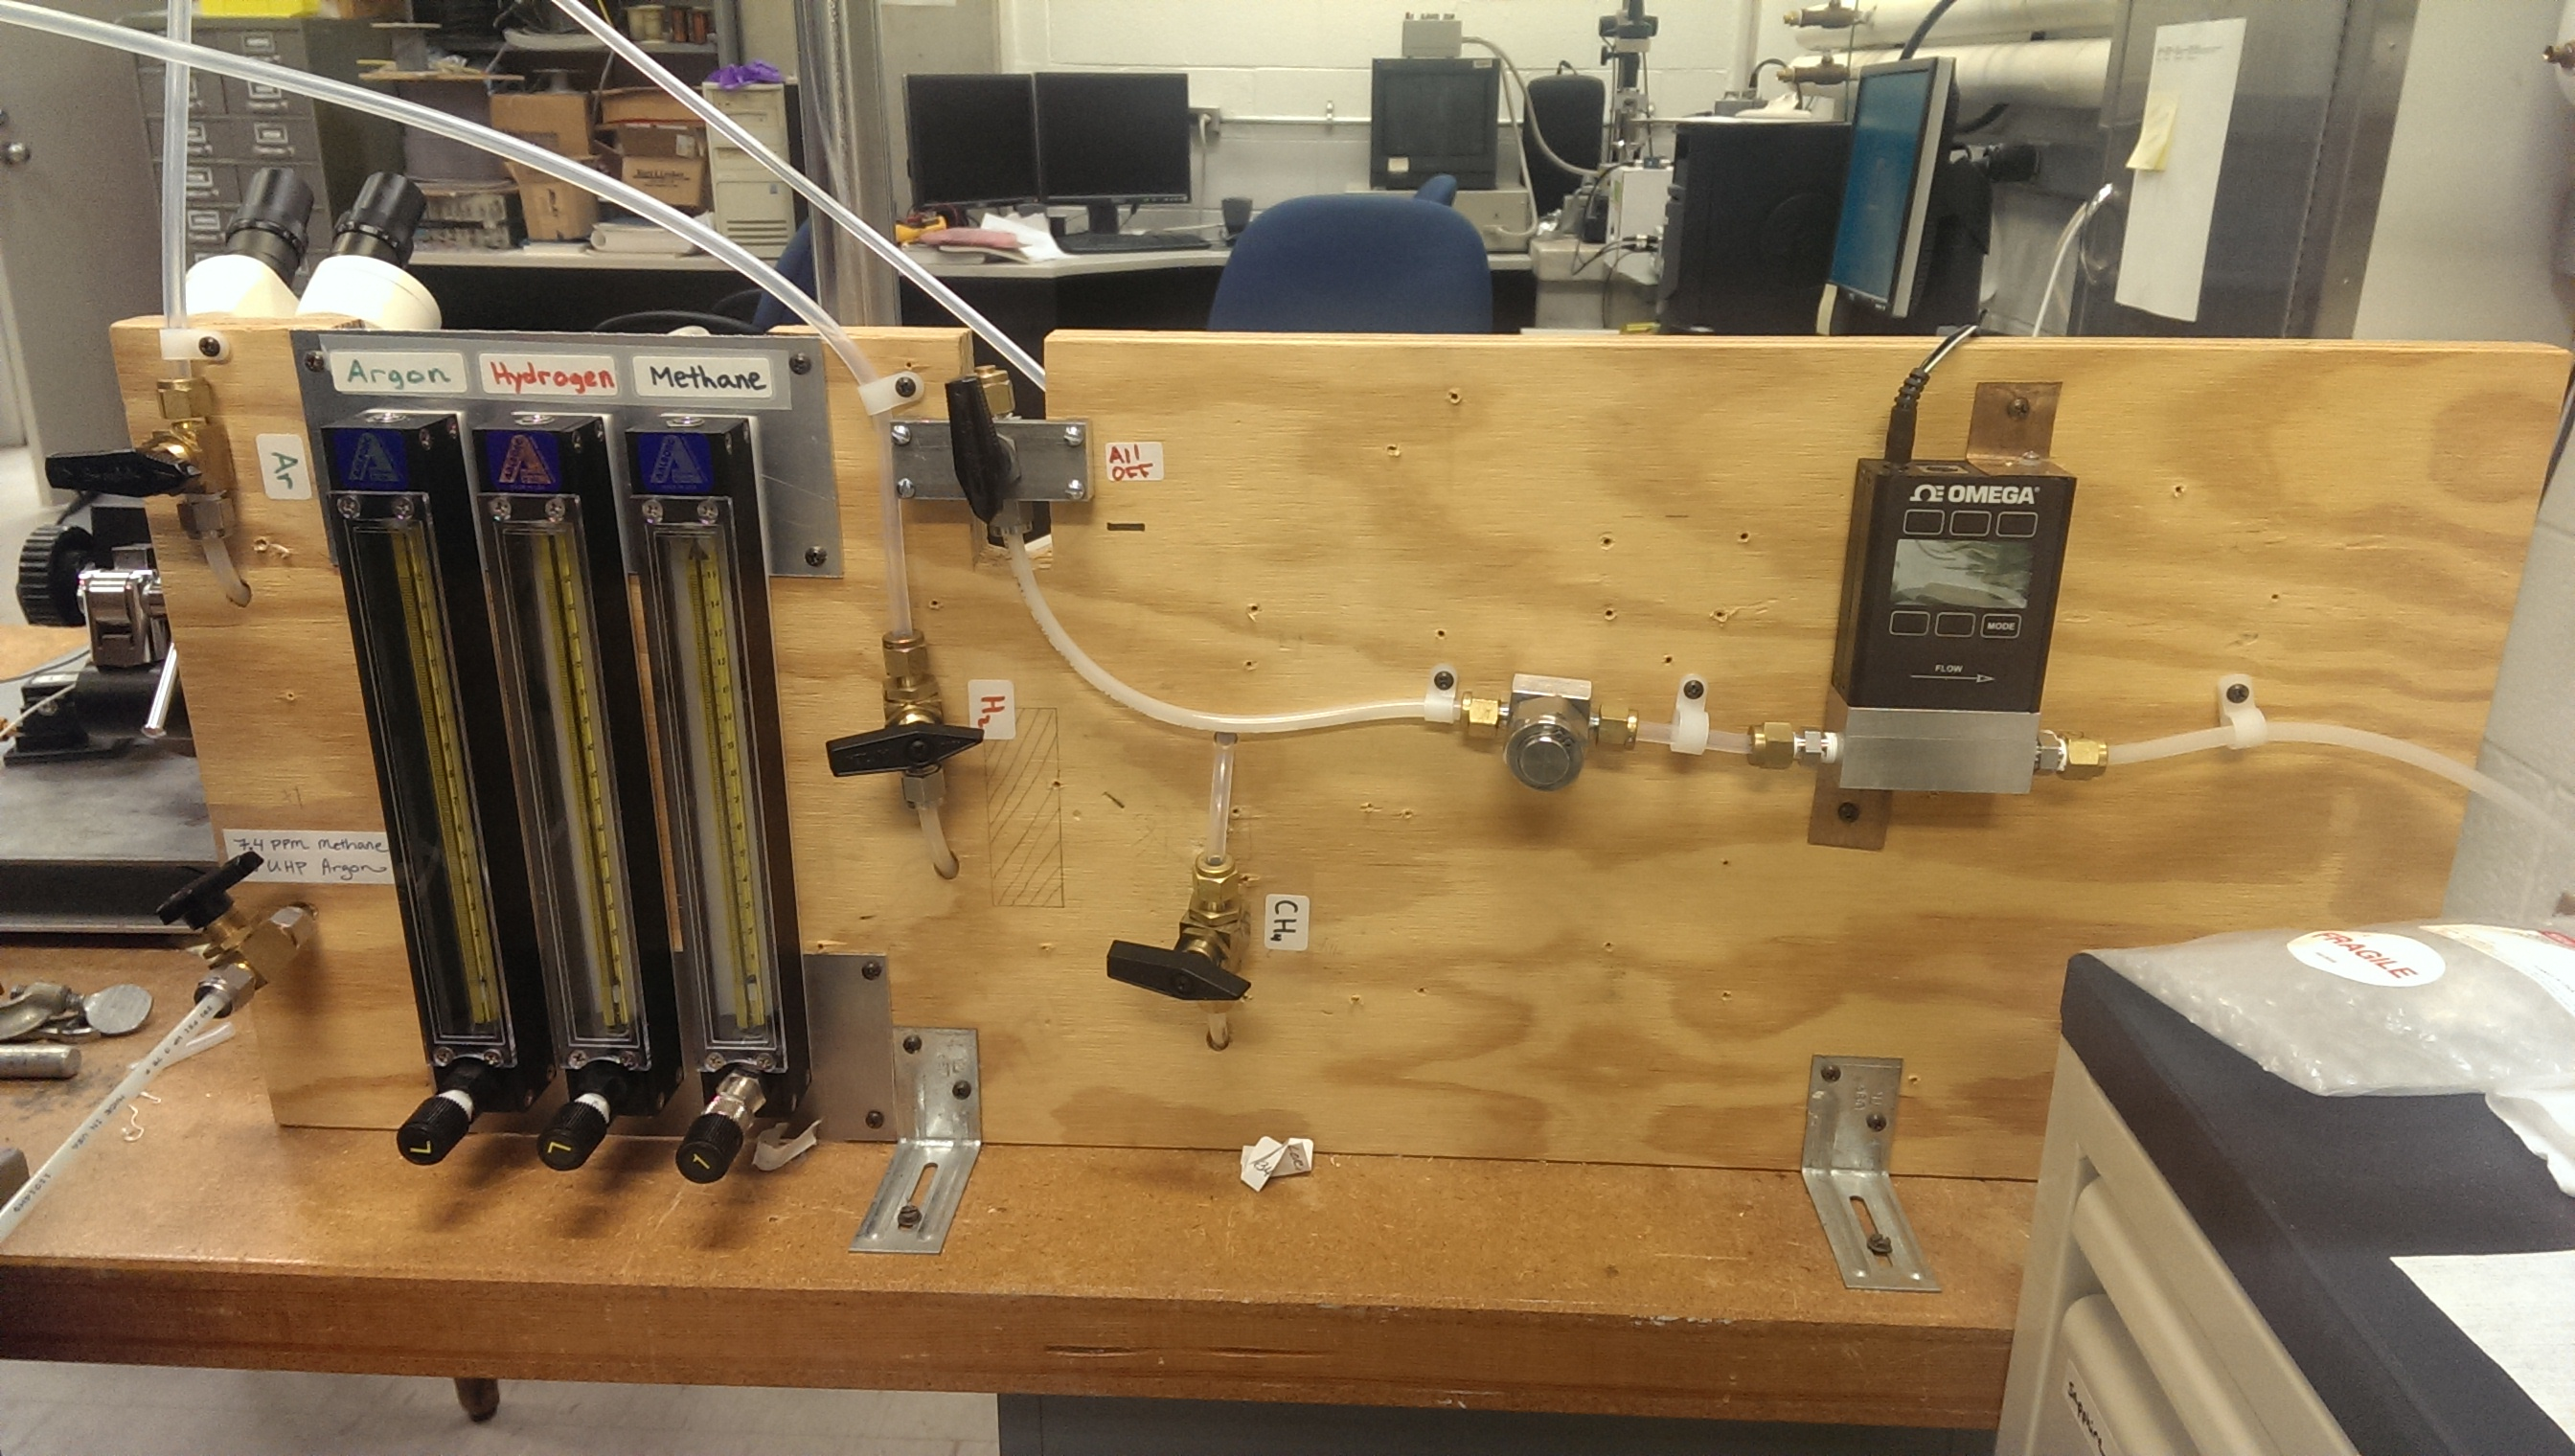
\includegraphics[width = 0.8\textwidth]{chapter3/gas_panel.jpg}
    \caption{The gas handling panel for our Lindberg tube furnace. Gas flow is from left to right.}
    \label{fig:gas_panel}
\end{figure}

The growth procedure begins with filling a ceramic crucible with the iron catalyst described in \ref{subsec:disperse_catalyst}. The catalyst should be spread in a thin layer across the bottom of the crucible, which is then loaded into the center of a 2-4 foot long quartz tube. The tube is sealed at each end, one side connected to the gas handling panel, and the other connected to the mineral oil filter and building exhaust. Our standard nanotube growth recipe is as follows: 

%can i remove the spacing from between these list items?
\begin{enumerate}
	\item Purge the tube by flowing \SI{2000}{\sccm} of Ar for 20 minutes
	\item Heat tube to \SI{1000}{\degreeCelsius} while flowing \SI{1000}{\sccm} Ar and \SI{200}{\sccm} \ce{H2}
	\item Flow \SI{2000}{\sccm} \ce{CH4} and \SI{200}{\sccm} \ce{H2} for 10 minutes.
	\item Set temperature to \SI{0}{\degreeCelsius} and let the furnace cool while flowing \SI{1000}{\sccm} Ar and \SI{200}{\sccm} \ce{H2}
\end{enumerate}

\noindent The actual nanotube growth occurs during the methane flow step. The \SI{200}{\sccm} \ce{H2} flow can be omitted, but it does seem to help promote nanotube growth. The flow rates do not need to be precise. Most nanotubes grow in the first few seconds of methane flow regardless of the flow rate. The Ar and \ce{H2} are simply to keep \ce{O2} and \ce{H2O} out of the tube. 

\subsection{Nanotube Placement}

After the CVD process, the nanotubes remain attached to the iron\slash alumina\slash molybdenum catalyst particles, which must be removed before depositing onto a silicon substrate. The nanotube\slash catalyst powder is first scraped from the ceramic crucible used in the tube furnace. The powder is then mixed with either dichloroethane or dichlorobenzene in a \SI{1}{\milli\gram} to \SI{10}{\milli\liter} ratio. Dichlorobenzene has been found to leave less residue after deposition, but may promote more damage to nanotubes during sonication. This was noted by Justin Silverman, an undergraduate working with our lab on functionalizing short carbon nanotubes. Some attempts were made to use water along with the surfactant SDS. However, SDS turned out to be difficult to remove and no devices were made in this way.

To remove the catalyst particles from the nanotubes, the solution described above must be placed in an ultrasonic bath for 1-60 minutes. The amount of time needed varied a great deal depending on the equipment and solvent used. The goal of this step is to break up large pieces of catalyst, separate nanotube bundles, and break individual nanotubes away from their catalyst particles. Sonication can be stopped when no large pieces of catalyst\slash nanotube material are visible and the solution has a uniform black color. Leaving the solution in the sonicator for too much time will begin to break long nanotubes. This may be somewhat beneficial in breaking nanotubes at defects that might otherwise affect transport measurements.

When sonication is complete, the solution is transferred to a centrifuge. This step is intended to precipitate the loose catalyst particles from the solution, while leaving the much lighter nanotubes suspended. The centrifuge used in our lab runs at \SI{2200}{\rpm} and nanotube solutions are left inside for 5-10 minutes. Once the centrifuge stops, the precipitate is discarded and the supernate, containing the suspended nanotubes, is reserved. We also tested using a high-speed, air-powered centrifuge running at \SI{100000}{\rpm} to separate nanotubes and catalyst. This did lead to much better catalyst separation and cleaner results,.

Now the solution is ready for deposition on a silicon substrate. The substrates are typically pre-patterned with a set of reference markers placed by optical (\ref{subsec:optical}) or electron beam lithography (\ref{sec:ebeam_lith}). An example of a patterned substrate can be seen in Figure \ref{fig:markers}

\begin{figure}
    \centering
    \includegraphics[width = 0.8\textwidth]{chapter3/markers.eps}
    \caption{A \ce{Si}/\ce{SiO2} substrate with \SI{1}{\micro\meter} \ce{Au} markers. Left scale bar: \SI{100}{\micro\meter}. Right scale bar: \SI{20}{\micro\meter} }
    \label{fig:markers}
\end{figure}

\subsection{Advantages and Disadvantages}

Despite having some success fabricating devices using randomly dispersed nanotubes and electric force microscopy scans (Section \ref{subsec:EFM}), the process was found to be too time consuming for frequent use. The main failure point was the preparation of nanotube solutions after growth. The concentrations varied significantly, often producing samples with dense nanotube coverage or no nanotubes found in the regions imaged. Additionally, the process of making a suspended nanotube solution is time consuming. Even those solutions with a useful concentration of nanotubes only remain fully suspended for less than 1 hour. Meaning the process must be repeated frequently.

\section{Catalyst Island Growth}
\label{sec:catalyst_island}

In 1998 \cite{Kong1998a}, it was discovered that the same type of catalyst used to grow nanotubes in powder form (Section \ref{subsec:disperse_catalyst}), could be suspended in solution, patterned, and used to grow nanotubes directly on silicon substrates. When paired with high melting point metals and optical lithography, nanotubes can be grown directly on patterned substrates in known locations. Devices prepared this way take just a fraction of the time to produce. However, these devices were found to be much more prone to other modes of failure, such as leaks in the gate oxide, amorphous carbon contamination on the substrate from the CVD growth process, and defects along the nanotube length.

\subsection{Catalyst} 

Many different types of catalyst particles can be used in the growth of carbon nanotubes. The ideal catalyst for patterned growth must be compatible with electron beam or optical lithography. Table \ref{table:catalysts} lists most of the catalysts tested in the Markovic lab. To test each catalyst, sputtered molybdenum leads were patterned using the mask aligner and Futurex NR9 resist. Catalyst islands were then patterned using electron beam lithography. Figure \ref{fig:catalyst_islands} shows an example of a substrate with Mo leads and catalyst islands.

\begin{figure}
	\centering
	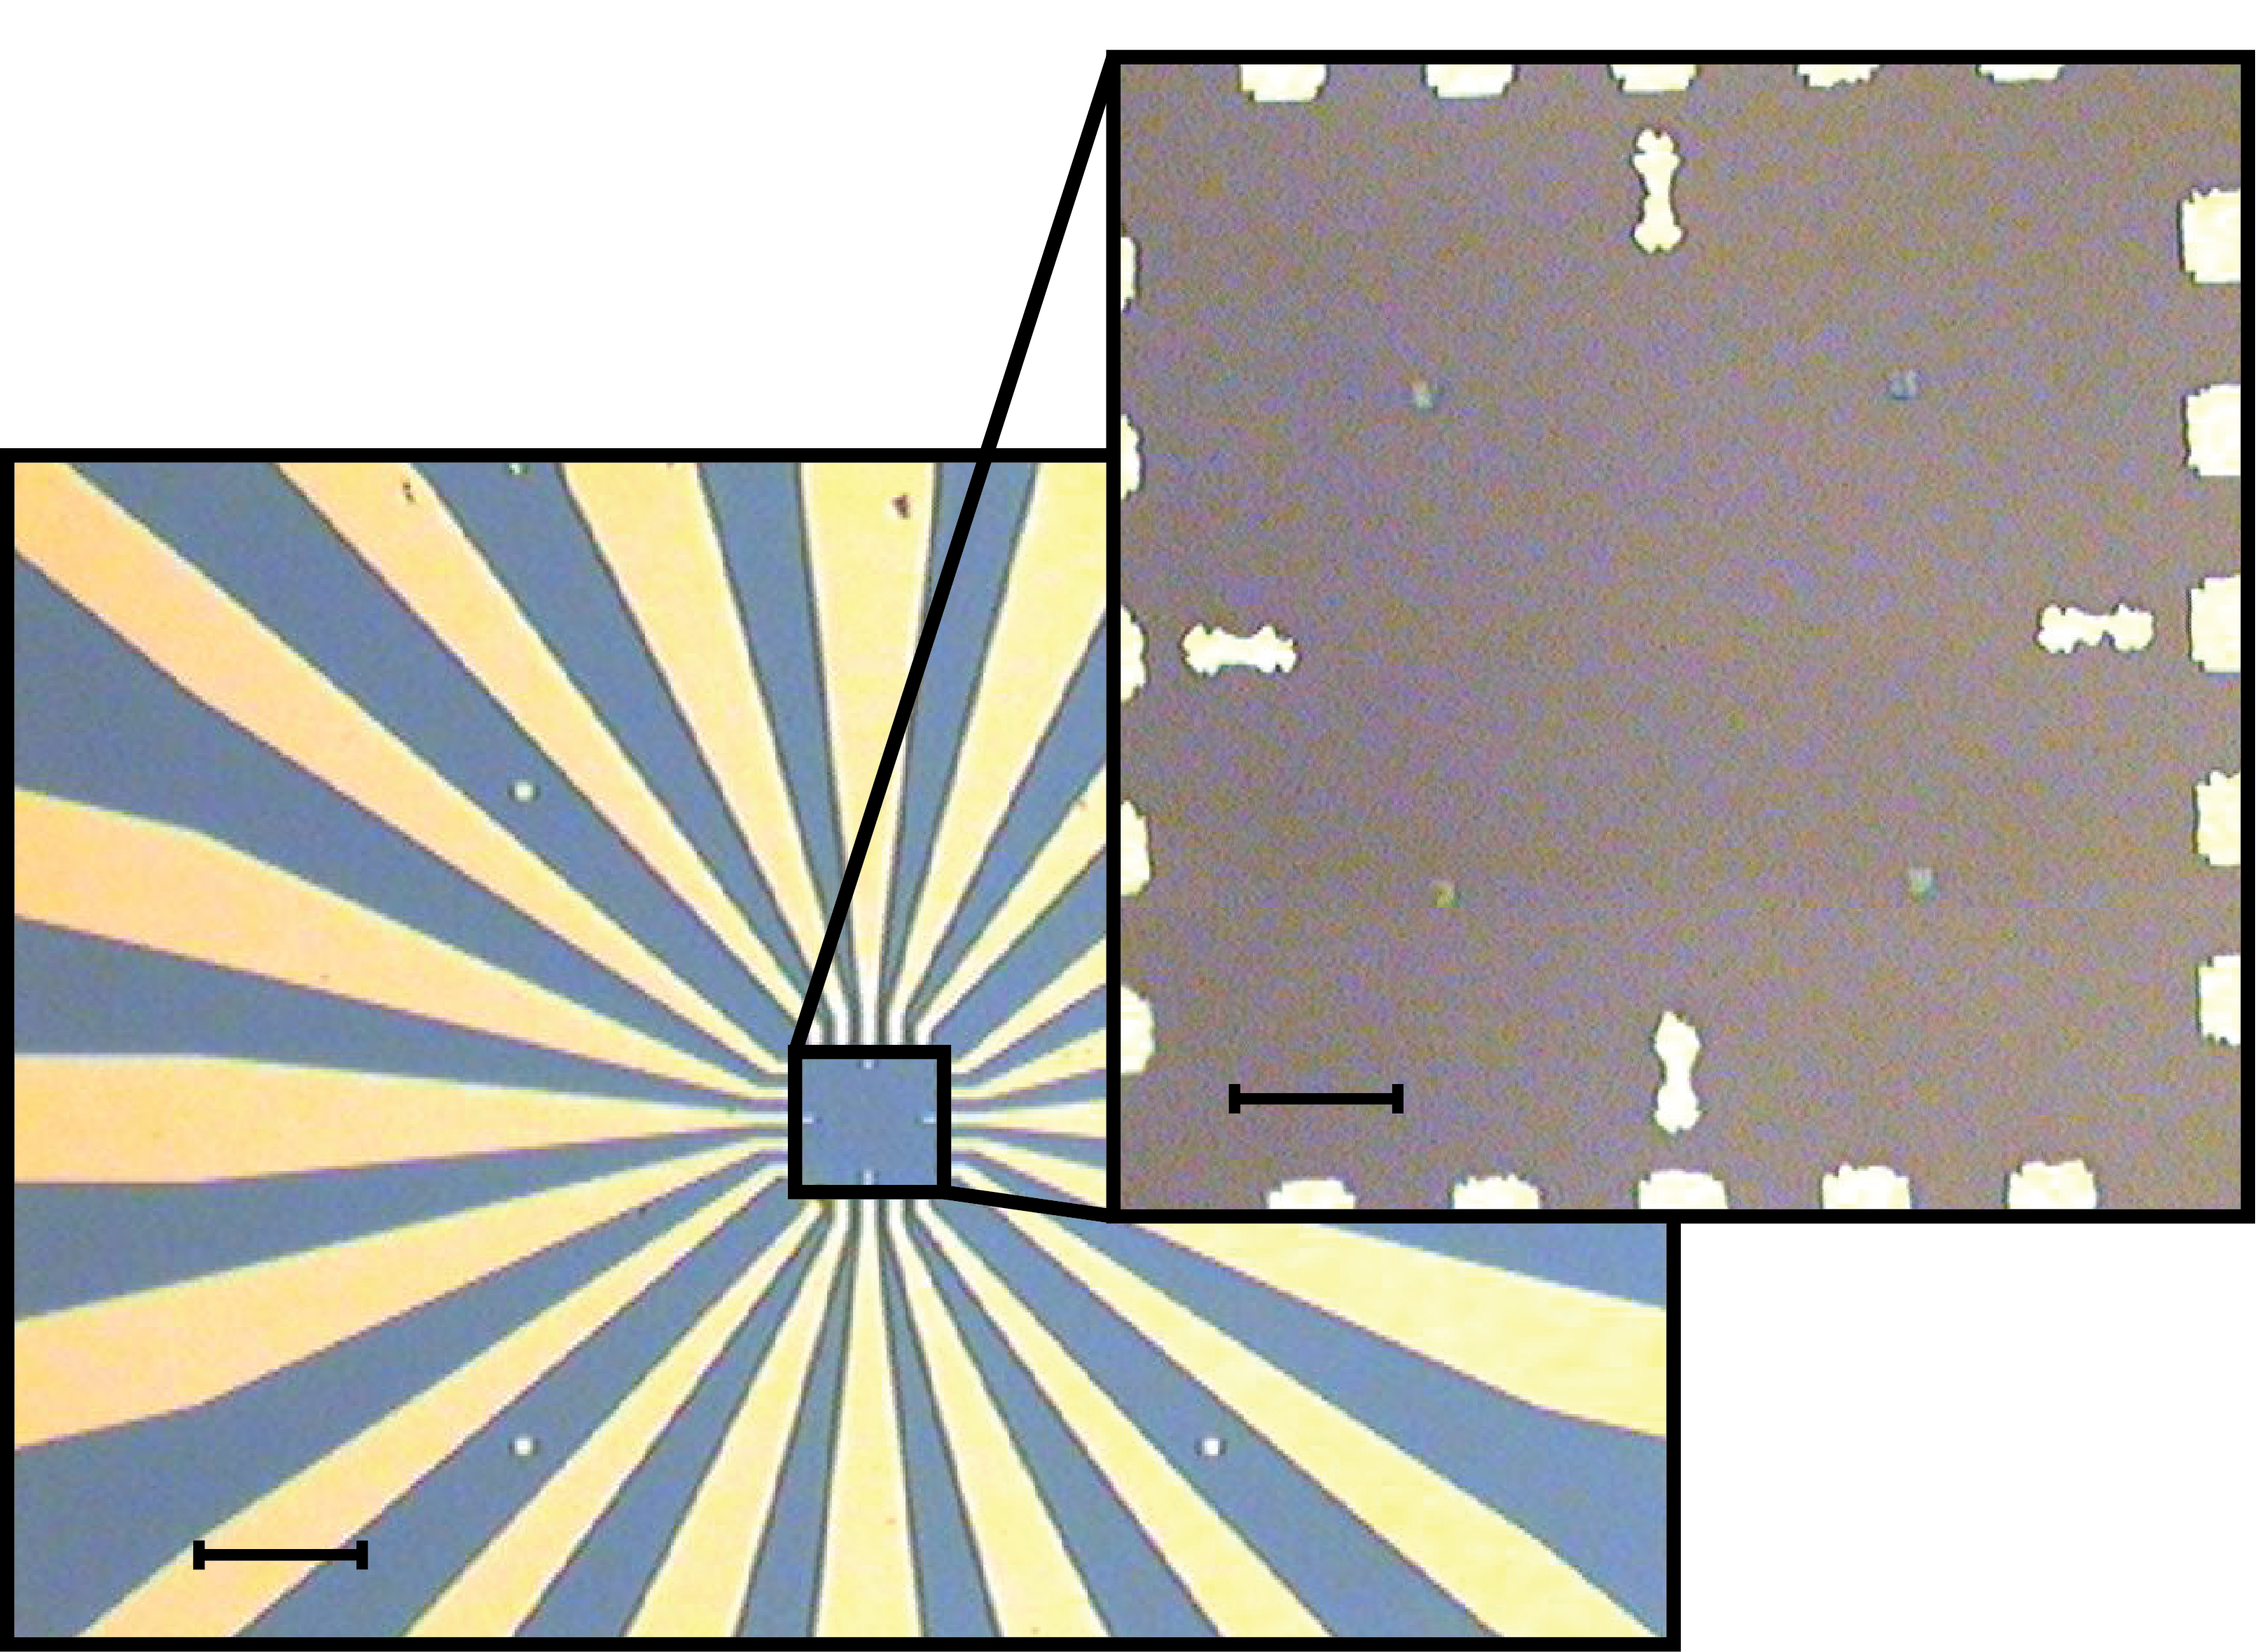
\includegraphics[width = 0.8\textwidth]{chapter3/catalyst_island.eps}
	\caption{A \ce{Si}/\ce{SiO2} substrate with \SI{3}{\micro\meter} catalyst islands and \ce{Mo} leads. Left scale bar: \SI{100}{\micro\meter}. Right scale bar: \SI{20}{\micro\meter} }
	\label{fig:catalyst_islands}
\end{figure}

\begin{table}
	\centering
	\caption{Patterned Catalysts}
    \begin{tabular}{| r | c || p{70mm} |}
    	\hline
    	\textbf{Catalyst} & \textbf{Suspended In} & \textbf{Results} \\ \hline
        Fe/Mo/alumina \cite{Kong1998} & Methanol & Easy to pattern. Liftoff difficult. Slowly attacks PMMA mask. Appeared to promote gate leaks through the \ce{SiO2} layer. \\ \hline
        Fe/Mo/alumina \cite{Aurich2012} & IPA & Poor adhesion to substrate. \\ \hline
        Fe/Mo/alumina \cite{Ouellette2008} & DI water & Easy to pattern. Excellent adhesion. No gate leak problems. \\ \hline
        \ce{FeCl3} \cite{Hong2005} & DI water & Excellent adhesion to substrate. Not compatible with PMMA mask. Left substrate entirely covered in catalyst. May work well with PDMS stamp. \\ \hline
        thermally evaporated Fe \cite{Biercuk2004, Kang2007} & None & Very easy to pattern. Liftoff is clean. Difficult to control the thickness below \SI{1}{\nano\meter} as required. \\ \hline
    \end{tabular}
    \label{table:catalysts}
\end{table}

All of the devices discussed in this thesis were produced using the Fe\slash Mo\slash alumina catalyst suspended in water. The islands were patterned using electron beam lithography. Catalyst is deposited in the following way:

\begin{enumerate}
	\item Add the powder catalyst from Table \ref{table:powder_catalyst} to \SI{15}{\milli\liter} of DI water and stir for 12 hours
	\item Sonicate the solution for 30 minutes
	\item Cover the sample in catalyst solution for 30 minutes
	\item Dry with \ce{N2} gun
	\item Liftoff by sonicating in acetone for 5 minutes, soaking in a clean acetone for 5 minutes, followed by an isopropanol rinse for 1 minute and a DI water rinse for 1 minute
\end{enumerate}

Obtaining reproducible results in the catalyst deposition was the source of much difficulty. The recipe provided here can be repeated before liftoff shows insufficient catalyst coverage on the substrate. Additionally, it is suspected that baking the catalyst on a hot plate to dry the solution leads directly to gate leaks in the \ce{SiO2} layers and later device failure. Thus, there is no baking step in the deposition of our catalyst islands.

\subsection{Growth}
\label{subsubsec:substrate_cvd}

The recipe for on-substrate growth of nanotubes used in this thesis is very similar to the growth recipe for powder catalyst discussed in Section \ref{subsubsec:powder_cvd}. This recipe was developed over the course of several years from many points of reference \cite{Kong1998, Kong1998a, Dirks2010, Huang2003, Huang2004, Zhang2013, Hong2005} and a my own notes. The recipe is optimized for the 1 inch Lindberg tube furnace as seen in Figures \ref{fig:furnace_setup} and \ref{fig:gas_panel}. Most samples are placed in a smaller \SI{1}{\centi\meter} diameter, 1 foot long quartz tube, then placed in the larger 1 inch diameter quartz tube. This was done to make the samples easier to load into the 1" tube, as well as to reduce turbulence in the gas flow across the sample \cite{Hong2005}. 

The standard nanotube growth recipe used in this work is below:

\begin{enumerate}
	\item Purge the tube by flowing \SI{2000}{\sccm} of Ar for 20 minutes
	\item Heat the tube to \SI{250}{\degreeCelsius} while flowing \SI{300}{\sccm} Ar and \SI{150}{\sccm} \ce{H2}
	\item Wait for at least 1 hour
	\item Heat the tube to \SI{700}{\degreeCelsius} while flowing \SI{300}{\sccm} Ar and \SI{150}{\sccm} \ce{H2}
	\item Wait for 10 minutes
	\item Heat tube to \SI{950}{\degreeCelsius} while flowing \SI{300}{\sccm} Ar and \SI{150}{\sccm} \ce{H2}
	\item Wait for the temperature to stabilize
	\item Flow \SI{700}{\sccm} \ce{CH4} and \SI{150}{\sccm} \ce{H2} for 10-15 minutes
	\item Set temperature to \SI{0}{\degreeCelsius} and let the furnace cool while flowing \SI{300}{\sccm} Ar and \SI{150}{\sccm} \ce{H2}
\end{enumerate}

In almost every test, this recipe has grown nanotubes successfully. Steps 2 and 3 are included to remove water vapor from the air that might have collected inside the quartz tube on humid days \cite{Dirks2010}. Steps 4 and 5 are meant to remove iron oxide from the iron nanoparticles that make up the catalyst. 

The most common point of failure in growth has been related to the patterned molybdenum leads/markers on the substrate. Molybdenum oxidizes rapidly at high temperatures. Therefore, any oxygen contamination in the tube during the growth process will form a \ce{MoO} layer that is then quickly removed by reacting with the high temperature \ce{H2} flow. This process repeats and can lead to the Mo leads being entirely etched away. Additionally, it has been found that opening the furnace too soon during cooling can lead to the Mo leads peeling off of the substrate. This appears to be caused by some super-heating due to IR radiation reflecting off of the surfaces of the sample and quartz tube. It is a strange phenomenon that is avoided by allowing the furnace to cool to less than \SI{300}{\degreeCelsius} before opening the lid. These problems could also be solved by using a different high temperature metal such as a W/Pt bilayer, common in many other nanotube projects. Molybdenum was chosen for this work because it is easy to sputter and much more affordable.

\subsection{Advantages and Disadvantages}

Growing nanotubes from catalyst islands near predefined leads and markers offers a large improvement in processing time over the method of random dispersion. Nanotubes produced with this method are longer, cleaner, and easier to locate. These improvements made this method the obvious choice for device fabrication. The main disadvantage found in this technique is the introduction of defects along the nanotube length due to growth along the substrate. Because of this, a large number of devices must be fabricated in order to find one with clean transport properties at low temperature.

\section{Imaging Nanotubes}
\label{subsubsec:imaging_disperse}

Nanotubes on a \ce{SiO2} surface can be located in a number of ways. This section will review a number of different methods, focusing on improvements made in the course of this thesis work.

\subsection{Atomic Force Microscopy}

With nanotubes that have been drop cast onto the surface, the standard method is to locate the tubes relative to the predefined markers using a tapping mode atomic force microscope (AFM). An example of an image created this way is seen in Figure \ref{fig:cnt_au_markers}. 

\begin{figure}
	\centering
	\includegraphics[width = 1.0\textwidth]{chapter3/single_cnt_au_markers.pdf}
	\caption{AFM height and amplitude scans of nanotubes dispersed over a substrate with \SI{1.5}{\micro\meter} gold markers. The scale bar is \SI{10}{\micro\meter}.}
	\label{fig:cnt_au_markers}
\end{figure}

This method is very reliable, but extremely time consuming. In order to resolve nanotubes, as well as the predefined markers in the image, AFM scan sizes must be limited to \SI{25}{\square\micro\meter}. Each of these scans takes 30 minutes and many scans are needed to fully image one patterned substrate. Looking closely at Figure \ref{fig:cnt_au_markers}, there are 12 scans covering less than half the substrate. Due to vibrational noise and piezo limits, some images are slightly warped. Stitching the images together is time consuming and inaccurate.

\subsection{Electric Force Microscopy}
\label{subsec:EFM}

The Digital Instruments Nanoscope 3 used in our lab is also capable of making electric force microscope (EFM) measurements. An EFM image is made by first measuring the height across the sample in standard tapping mode, then using that height data to run a second 'interleave' scan at a fixed height with a bias voltage applied between the tip and sample. By holding the tip at a fixed height, van der Waals interactions between the tip and sample are constant and the only force measured is the electrostatic force from the applied bias voltage. Contrast in the resulting images is related to the different conductivities of the objects on the sample \cite{Bockrath2002}. Thus, conducting (and semiconducting) nanotubes have a high contrast against the insulating \ce{SiO2} substrate. An example of this type of image is shown in Figure \ref{fig:cnt_efm}

\begin{figure}
	\centering
	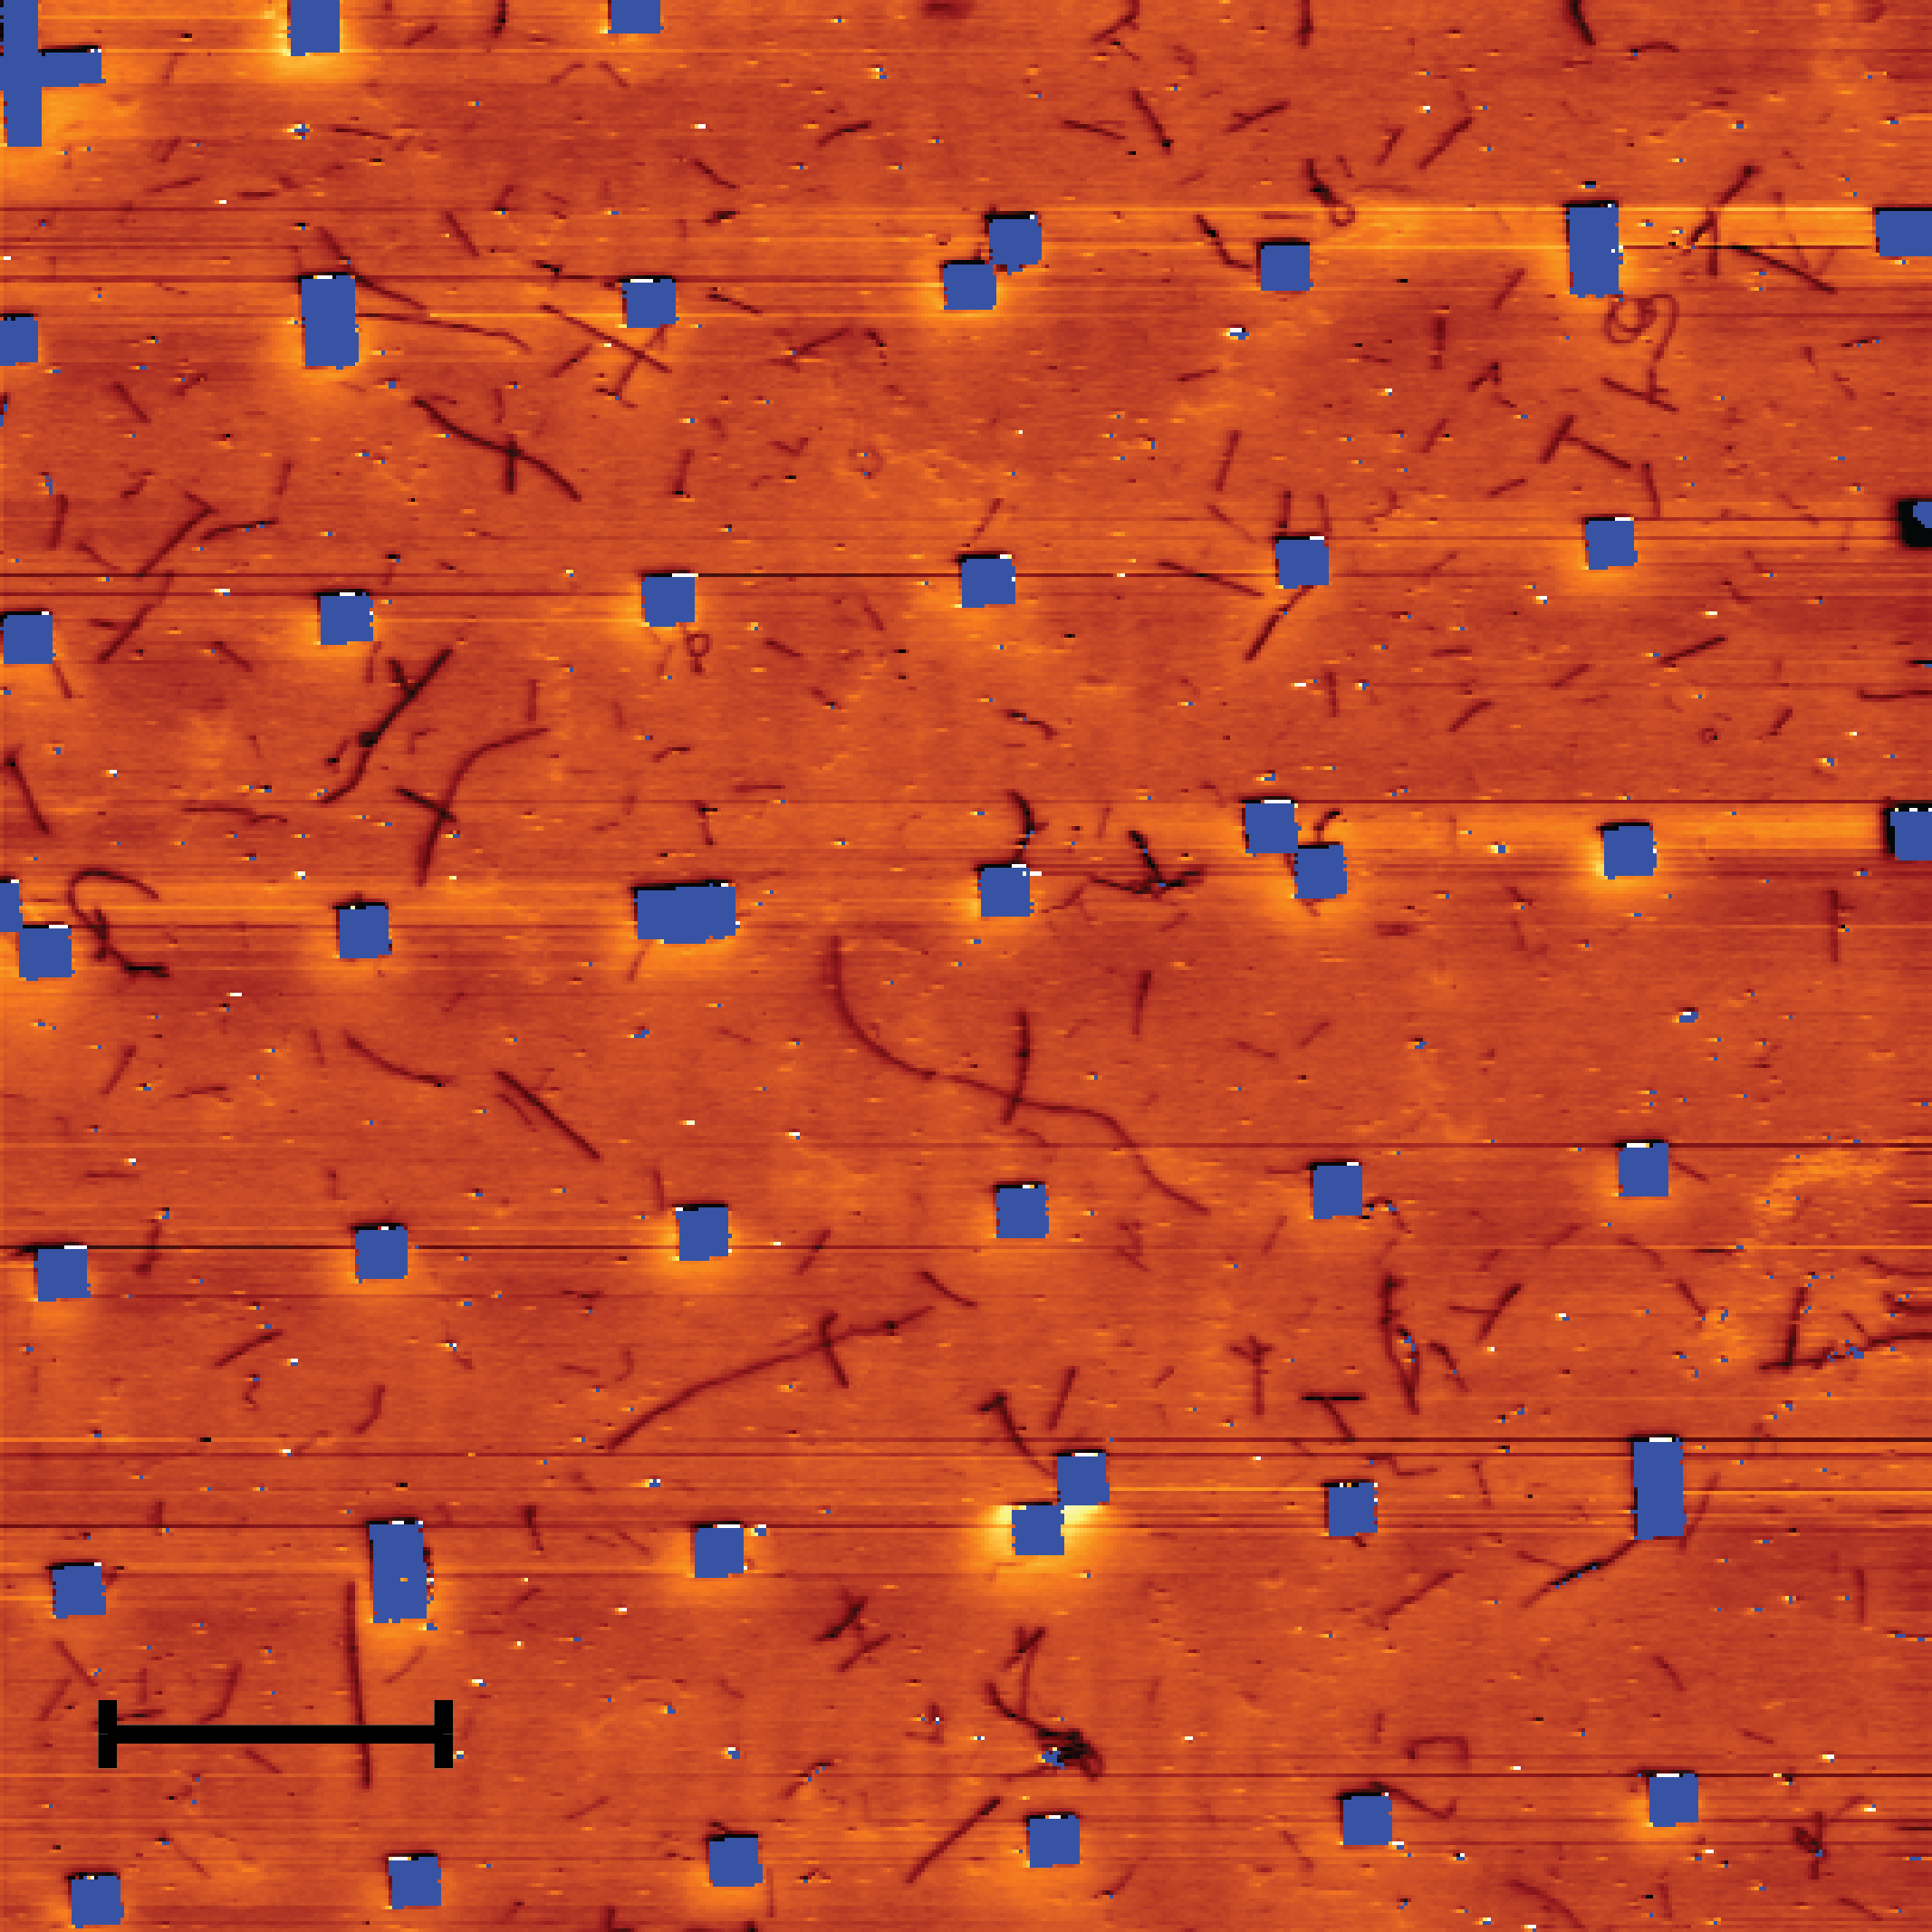
\includegraphics[width = 0.8\textwidth]{chapter3/cnt_efm.eps}
	\caption{An EFM image of nanotubes dispersed over a substrate with \SI{1.5}{\micro\meter} gold markers. The markers have been automatically located using the height data and highlighted in blue on the EFM image. The scale bar is \SI{10}{\micro\meter}.}
	\label{fig:cnt_efm}
\end{figure}

An entire patterned substrate can be scanned using this method in about 1 hour. The scan size can be increased up to \SI{75}{\square\micro\meter} due to the false contrast provided by the large electrostatic forces between the nanotubes and the tip. Rather than appearing as \SI{1}{\nano\meter} in diameter, the tubes appear in the EFM image to be about 100 times their real diameter. This was a notable improvement over locating nanotubes using AFM height scans alone. Comparing Figure \ref{fig:cnt_au_markers} and Figure \ref{fig:cnt_efm}, it is clear the EFM image is far more useful in locating nanotubes.

\subsection{EFM Through PMMA}

All of the same techniques from Section \ref{subsubsec:imaging_disperse} can be applied to imaging nanotubes grown from patterned catalyst islands. However, because the substrates are not covered in closely spaced markers, it was found that tapping mode AFM height scans were not useful. Scans could only cover a small part of the sample and the resulting images were difficult to orient.

Using electric force microscopy (EFM) made it possible to scan the entire region of interest on the sample in one measurement. An example of this type of scan is shown in Figure \ref{fig:efm_islands}a. As can be seen in that figure, it was difficult for the AFM tip to avoid crashing into the catalyst islands during the EFM sweep. The catalyst islands are several hundred nanometers in height while the other features on the substrate are less than \SI{10}{\nano\meter}. Such height differences make large area scans difficult in tapping mode. This problem can be avoided by coating the sample in PMMA before scanning with the EFM, as seen in Figure \ref{fig:efm_islands}b. The PMMA coating smooths the height differences between the substrate and catalyst islands, without compromising the contrast between the insulating substrate and conducting nanotubes. The idea was adopted from a 2007 paper in which the authors attempted to locate nanotubes suspended in a PMMA layer in three dimensions \cite{Jespersen2007}.

\begin{figure}
	\centering
	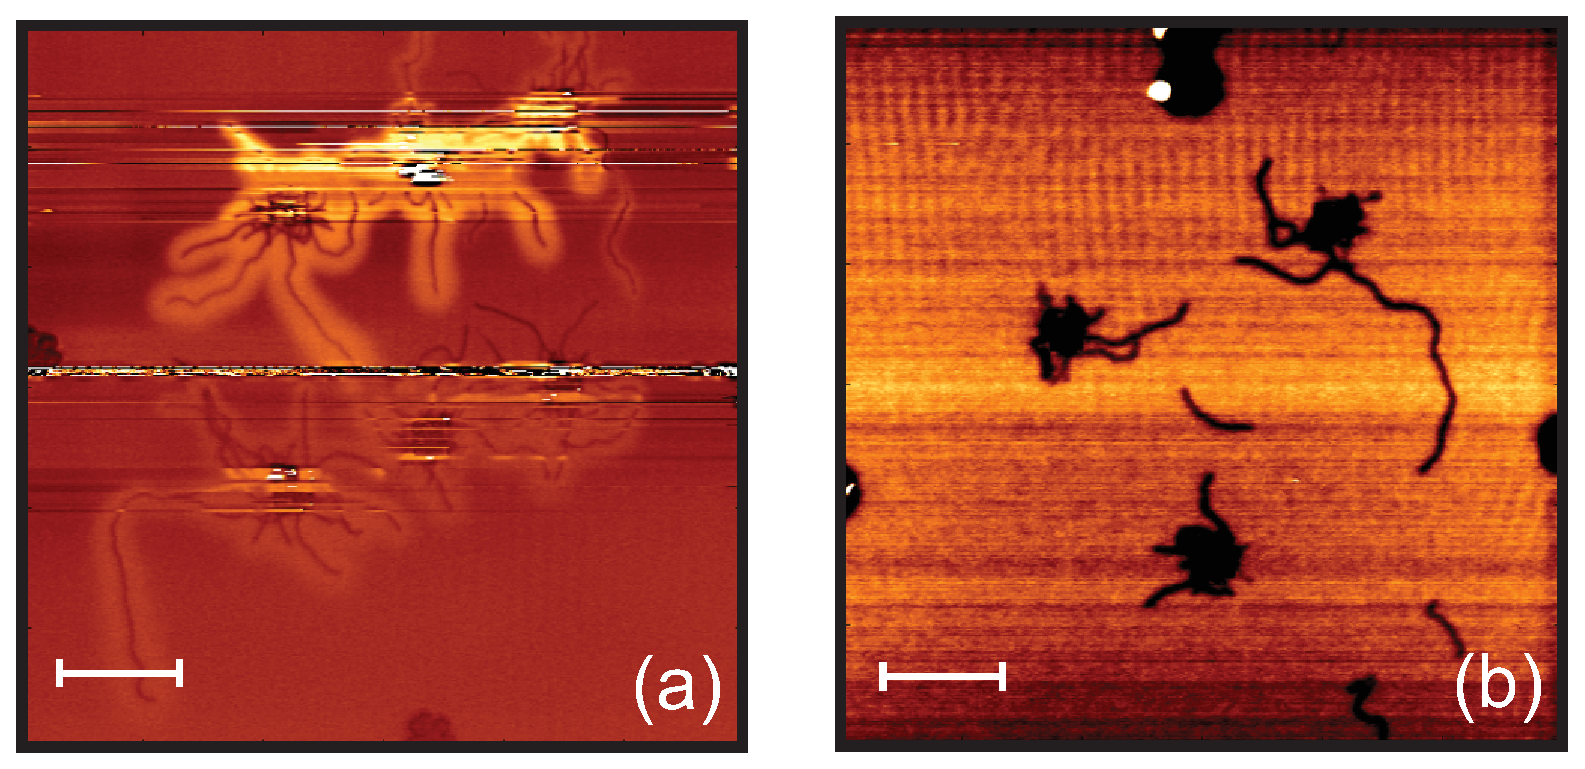
\includegraphics[width = 1.0\textwidth]{chapter3/efm_islands.eps}
	\caption{(a) Frequency data collected from an EFM scan of a catalyst island sample after nanotube growth. (b) Frequency data collected from an EFM scan of a similar sample. Prior to the scan this sample was coated with a \SI{250}{\nano\meter} PMMA layer. Both scale bars are \SI{10}{\micro\meter}. }
	\label{fig:efm_islands}
\end{figure}

\subsection{Scanning Electron Microscopy}
\label{subsec:imaging_sem}

In 2002, a paper \cite{Brintlinger2002} was published illustrating that a scanning electron microscope (SEM), operating at a low accelerating potential could provide a similar type of false contrast image as produced by the EFM. The insulating substrate tends to collect charge from the electron beam, while the conducting nanotubes do not. This produces an image in which the nanotubes appear as bright lines about 100 times their actual diameter. An example of this is seen in Figure \ref{fig:sem_islands}. 

\begin{figure}
	\centering
	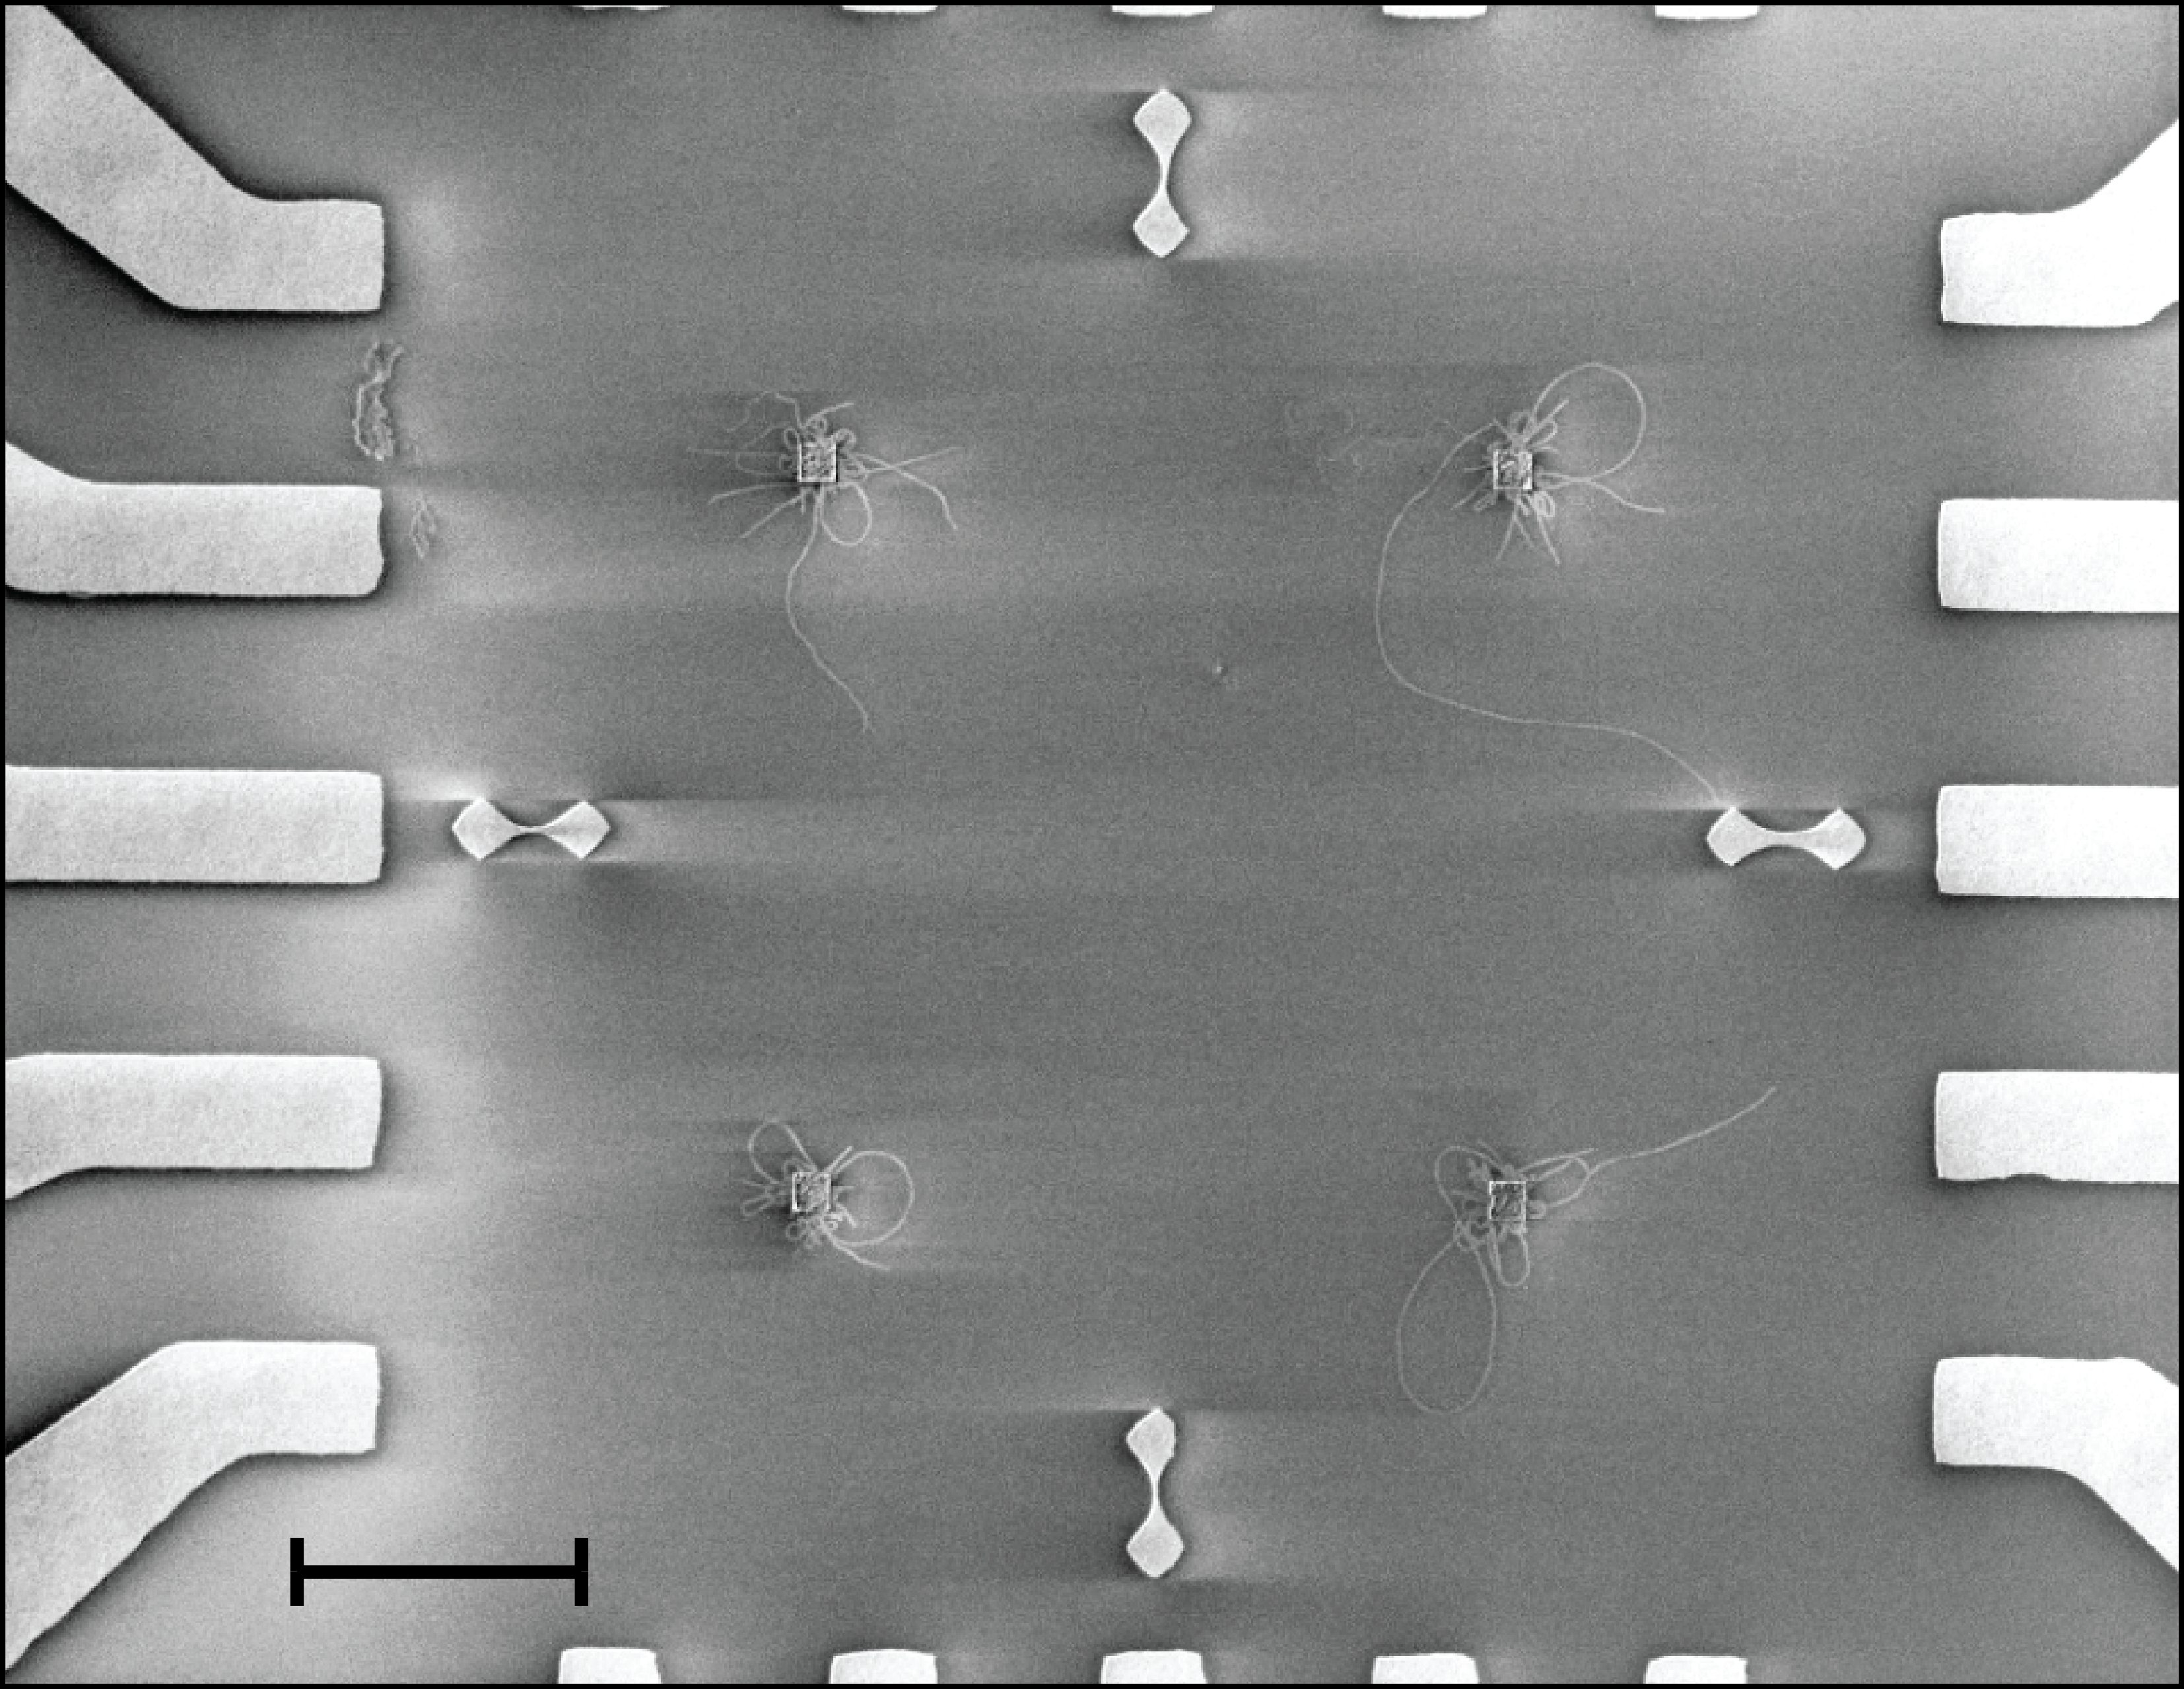
\includegraphics[width = 0.8\textwidth]{chapter3/sem_islands.eps}
	\caption{A scanning electron micrograph of a catalyst island sample after nanotube growth. The scale bar is \SI{10}{\micro\meter}.}
	\label{fig:sem_islands}
\end{figure}

Typically, an EFM scan of a sample will take 45 minutes. A SEM image of the same sample takes less than 2 minutes. However, the SEM can introduce some carbon contamination from the high energy electrons passing through small amounts of oil mist back-streaming into the vacuum chamber from the mechanical roughing pump. Due to the large number of samples that were produced to obtain the data in this thesis, it was decided that contamination from the SEM was an acceptable risk, given the immense time savings.

\section{Image Filtering}

Once it became clear that the scanning electron microscope was by far the most efficient and reliable way to locate carbon nanotubes on a substrate, it also became important to optimize those images to revel the most information possible. The resolution and contrast in the SEM images produced in our lab are limited by the the use of a thermionic \ce{LaB6} filament. Unlike field emission scanning electron microscopes, which are more common in nanofabrication, the thermionic scanning electron microscope has a large initial crossover size, requiring more electromagntic lens focusing to produce a sufficiently small beam size for imaging. This problem is exasperated when using low accelerating potentials (500-\SI{3000}{\volt}), which are crucial to achieving good contrast of carbon nanotubes on a silicon substrate.

\subsection{Histogram Equalization}

This method was based on two corrections. First, a plane fit to correct for the position of the secondary electron detector. Second, finding the histogram then transforming it such that there are equal numbers of pixels at each brightness level. An illustration of this can be seen in Figure \ref{fig:hist_eq}

\begin{figure}
	\centering
	\includegraphics[width = 0.4\textwidth]{chapter3/histogram_equalization_wiki.png}
	\caption{An illustration of the histogram equalization process.}
	\label{fig:hist_eq}
\end{figure}

Figure \ref{fig:hist_eq_data} shows the process of filtering an SEM image using histogram equalization. At the top of figure is the original image after a plane fit (to correct changes in brightness across the substrate). To the right of the image, the histogram of brightness values and the cummulative distribution function are plotted. The center image is after the histogram equalization. Contrast is now dramatically increased in the image, the histogram is nearly flat, and the cumulative distribution function is linear. Finally, the image is gaussian filtered using a $3 \times 3$ kernel to reduce the high frequency noise, which has been exaggerated by the histogram equalization. The final histogram is not flat quite flat and the cumulative distribution function is not quite linear. However, the contrast in the image has been enhanced significantly

\begin{figure}
	\centering
	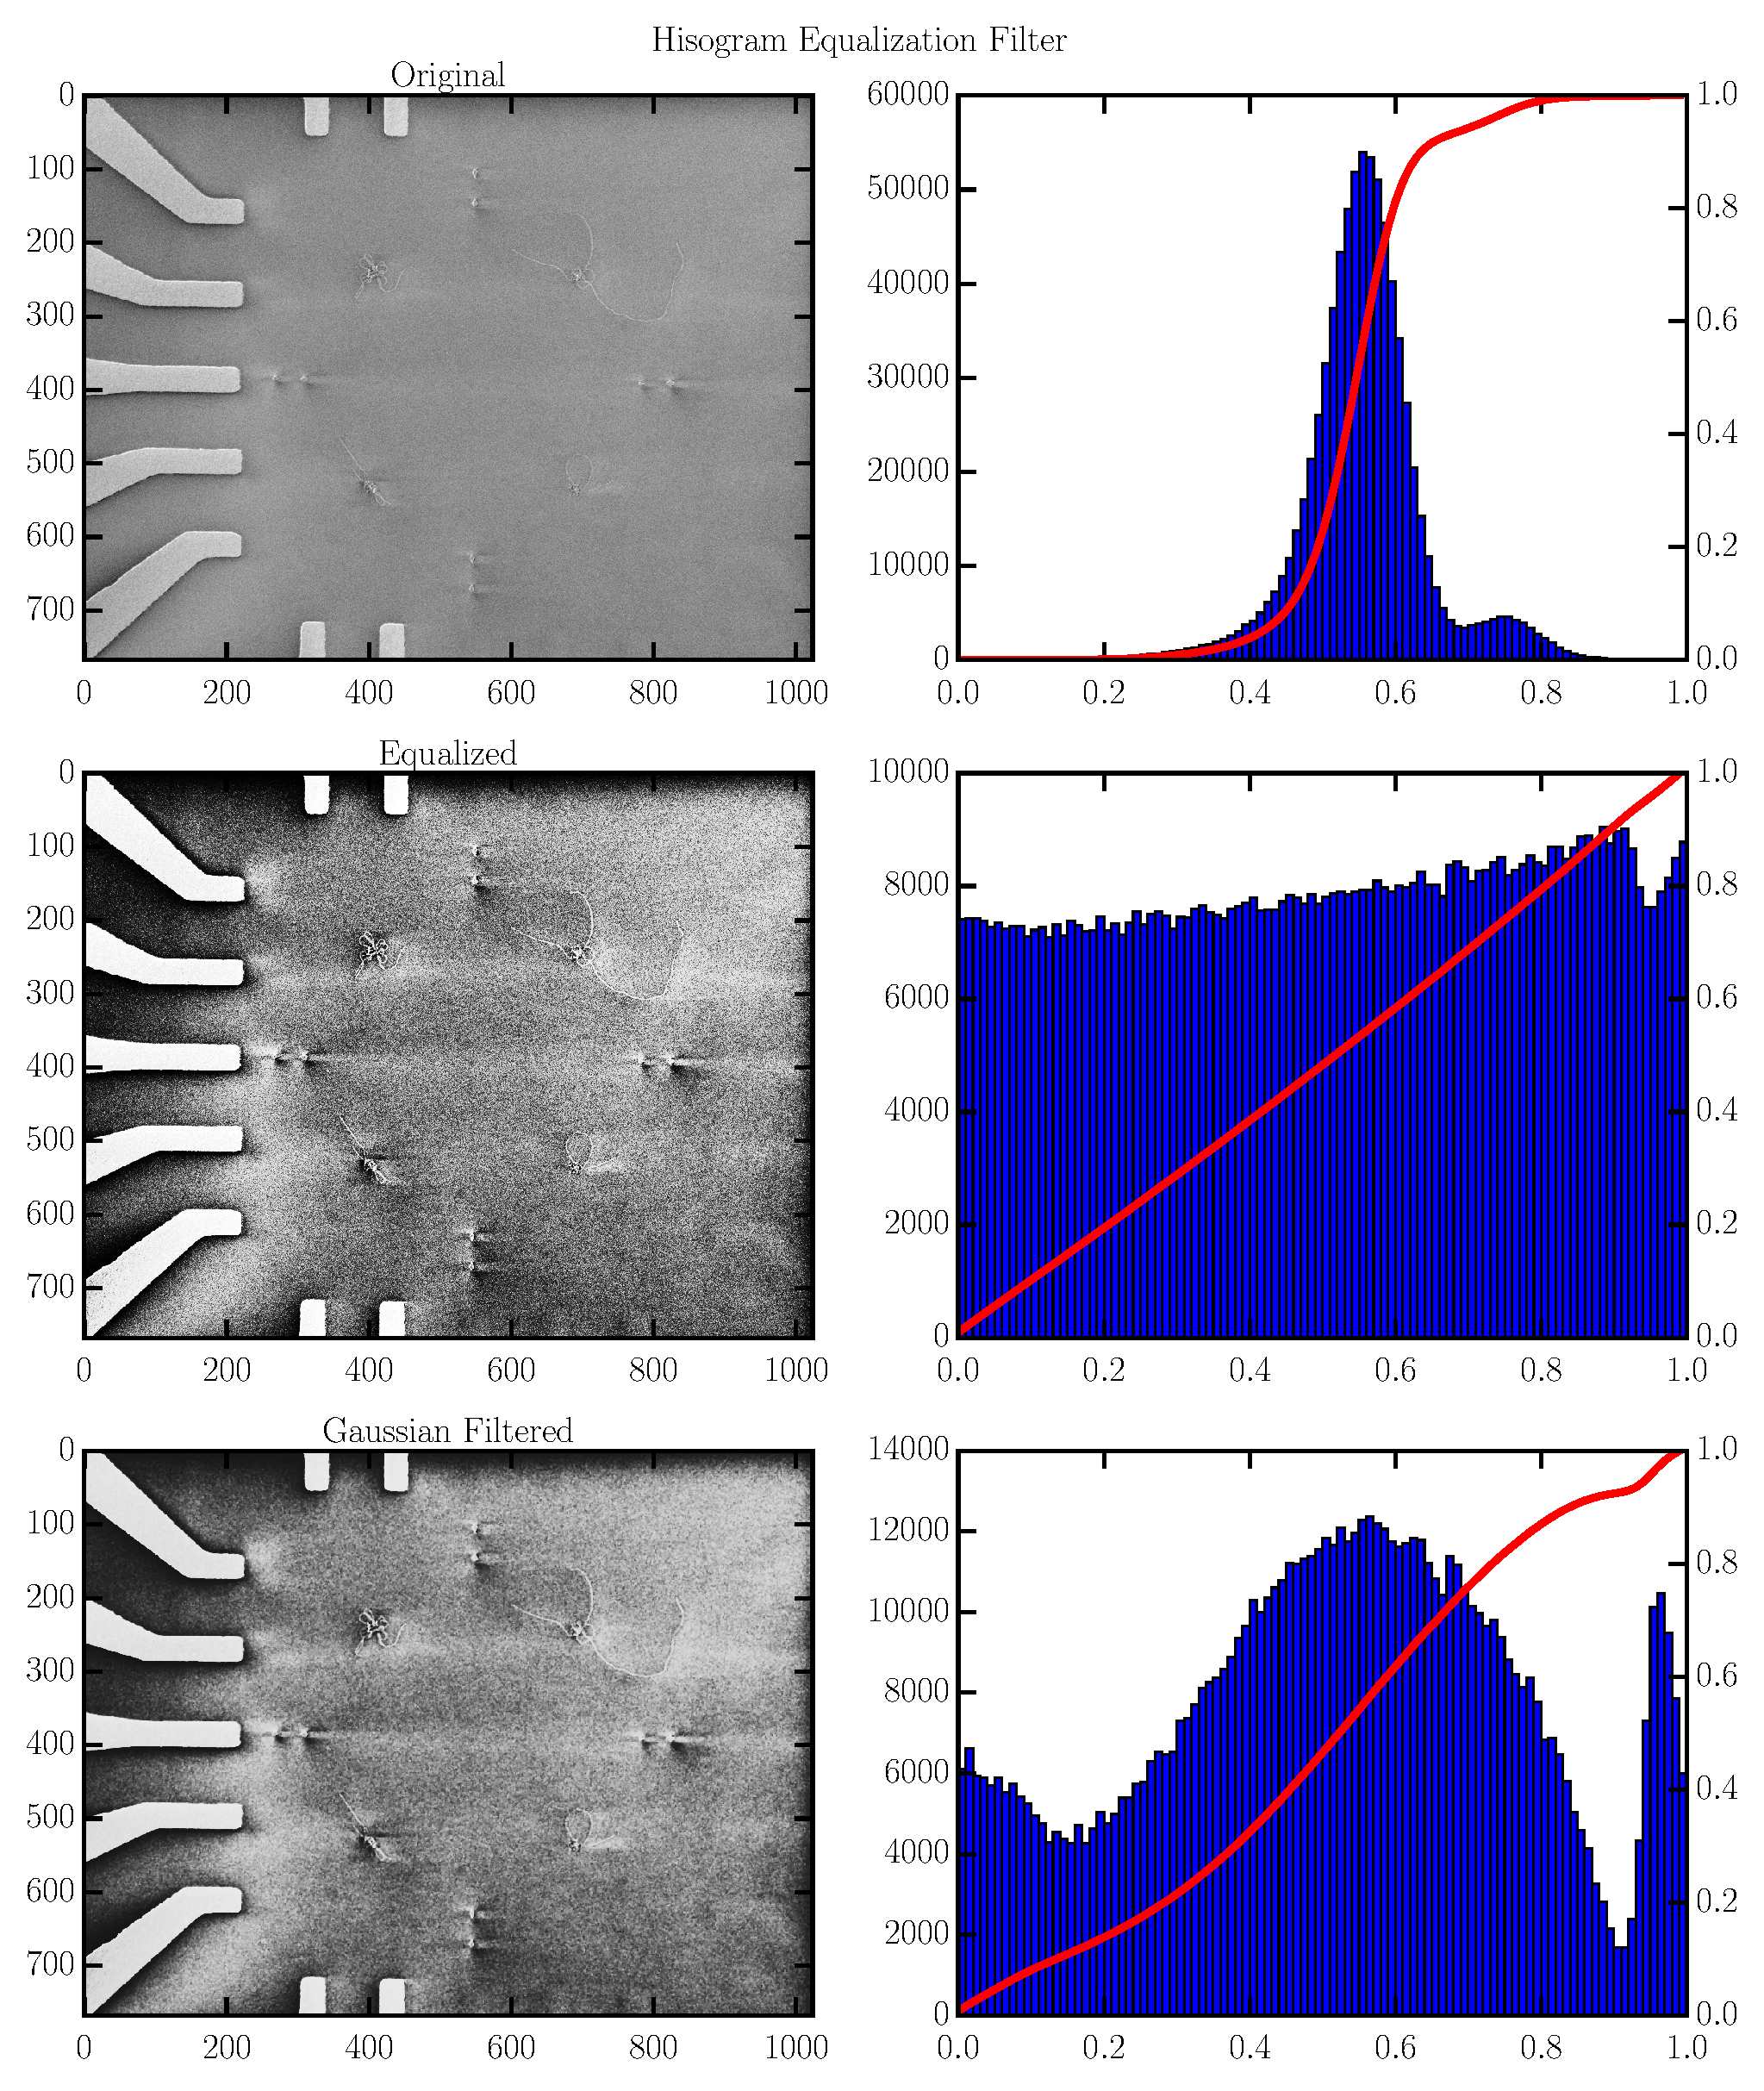
\includegraphics[width = 0.8\textwidth]{chapter3/histogram_eq_example.pdf}
	\caption{Top image is the original SEM image after a plane fit. Middle image shows the SEM image after histogram equalization. Bottom image shows the final result after gaussian smoothing. Plots on the right show the histogram of brightness values and cumulative distribution function at each step.}
	\label{fig:hist_eq_data}
\end{figure}

While this filter does succeed in increasing contrast in the image, which was the main problem associated with our SEM, it also increases the background noise to often unacceptable levels. Histogram equalization does not use any specific information about the carbon nanotubes and substrates being imaged. A better filter should be possible by taking advantage of the fact that the features of interest can be well characterized in a sample set of images. 

\subsection{Matched Filter Bank}

Matched filter banks are a well known technique that have been used very successfully to filter retinal images in medicine \cite{Chaudhuri1989}. This technique has previously been adapted to high resolution SEM images of carbon nanotube bundles \cite{Guerrero2014}. The following section describes the implementation of this method to filter images of single walled carbon nanotubes grown on insulating substrates. 
%% nanotube profiles -> kernel -> filtering/thresholding

\subsubsection{Nanotube Profile Model}

To begin building the matched filter bank, the profile shape of a single nanotube from the SEM image must be determined. To find this shape, a random set of 25 SEM images was selected (similar to those in Figure \ref{fig:sem_islands}). From each of these images, images of two nanotubes were cropped. Those nanobues can be seen in Figure \ref{fig:all_nanotube_sections}a. Each of these images was then rotated such that the longest straight portion (that could be identified by eye) was oriented vertically. The profile of the nanotube was averaged over that long straight section. These results are plotted in Figure \ref{fig:all_nanotube_sections}b.

\begin{figure}
	\centering
	\includegraphics[width = 1.0\textwidth]{chapter3/all_nanotube_sections.eps}
	\caption{a) The original data set of SEM nanotube images used to create and optimize the matched filter bank. b) The same data set rotated and overlaid with extracted nanotube profiles.}
	\label{fig:all_nanotube_sections}
\end{figure}

Based on the shape of these profiles a truncated $sinc$ function, Equation \ref{eq:sinc}, was chosen to fit the nanotube profile.

\begin{equation} 
\label{eq:sinc}
    f(x) = \begin{cases} \frac{A\sin{kx}}{kx} & |x| < \frac{2\pi}{k} \\ 
                         0                    & |x| > \frac{2\pi}{k} 
           \end{cases}
\end{equation}

This fuction was chosen because it captures the bright nanotube peak and dark regions beside the nanotube while still only requiring one fit parameter. To determine the fit parameters the linear background was subtracted from each profile in Figure \ref{fig:all_nanotube_sections}b and the profiles were  fit using \ref{eq:sinc}. The results of this fitting can be seen in Figures \ref{fig:profile_fits}a and b. 

\begin{figure}
	\centering
	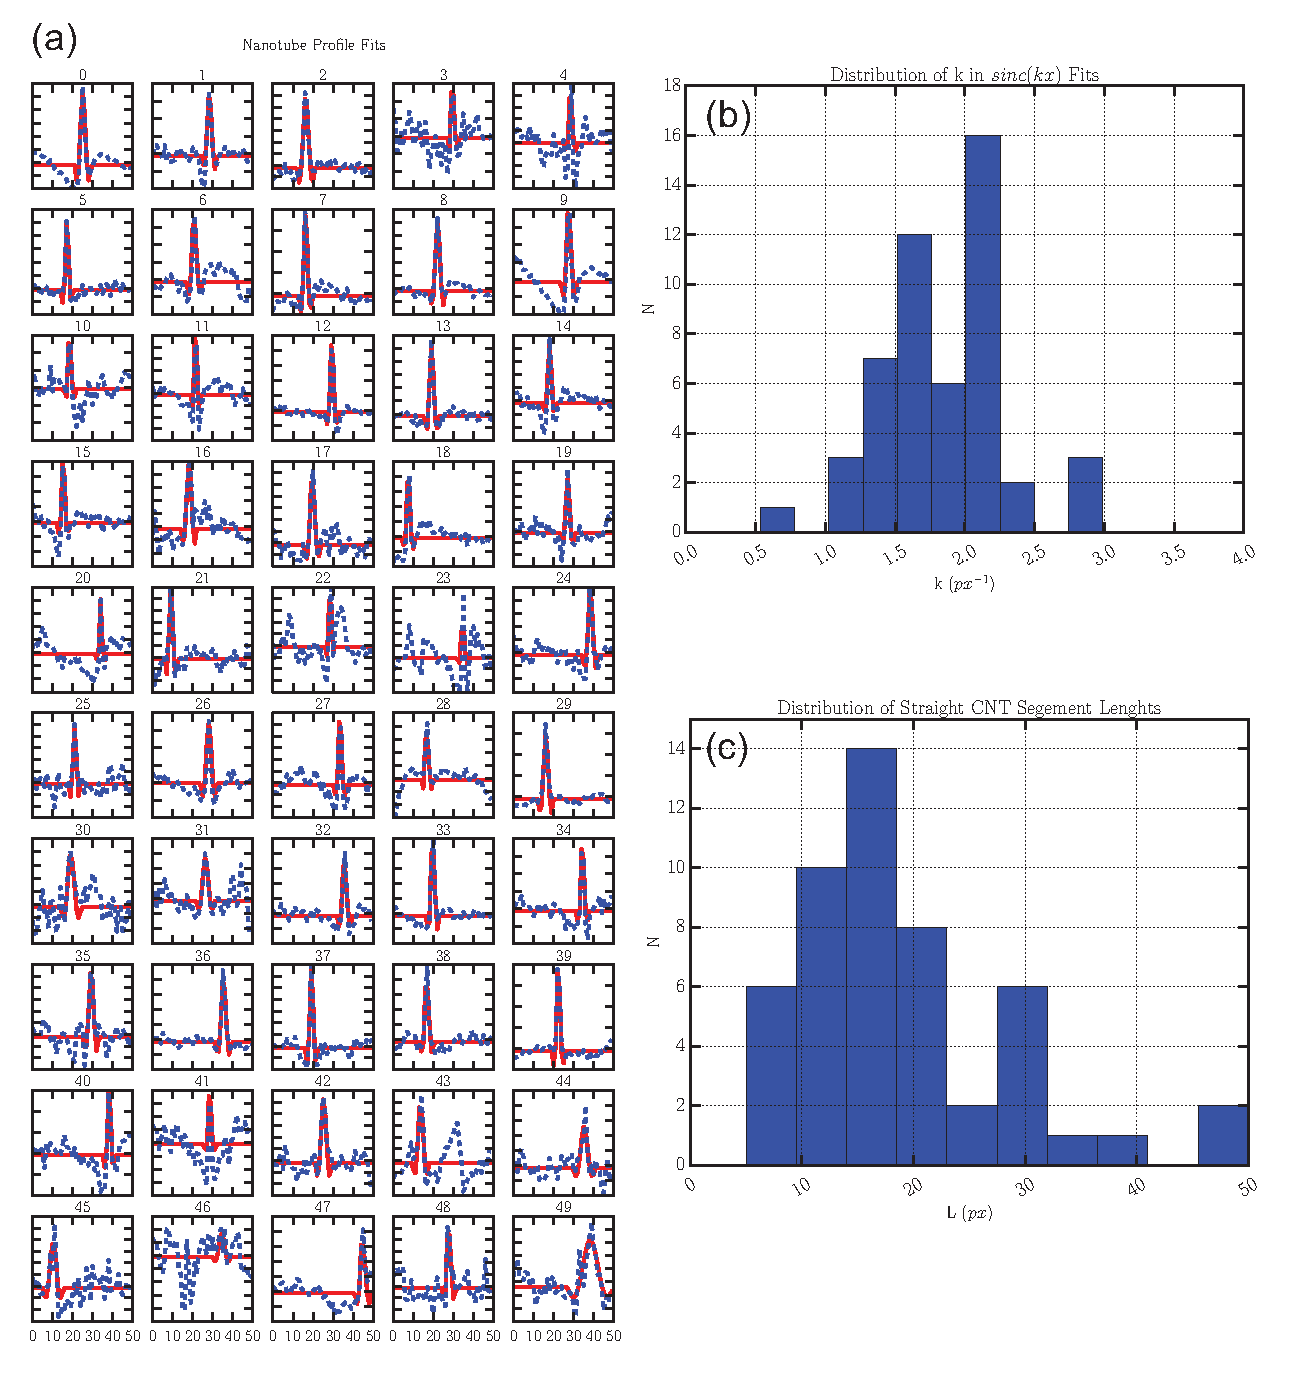
\includegraphics[width = 1.0\textwidth]{chapter3/profile_fits.eps}
	\caption{a) Extracted nanotube profiles with linear background removed (blue). Fits to \ref{eq:sinc} (red). b) Distribution of $k$ values extracted from profile fits. c) Distribution of straight nanotube section lengths.}
	\label{fig:profile_fits}
\end{figure}

\subsubsection{Filter Kernel}

The filter kernel is built starting with the median $k$ value found from the profile fits. To extract each profile, horizontal cuts of the nanotube image were averaged over a straight segment of the nanotube that was identified and labelled by hand. The distribution of these straight segment lengths can be seen in Figure \ref{fig:profile_fits}c. Again, to proceed with building the filter we use the median value of $L$ from that distribution. The kernel is built in an $N \times N$ matrix with $(x,y) = (0,0)$ at the center of the matrix. The full kernel, $K(x,y)$ is defined by Equation \ref{eq:kernel}.

\begin{equation} 
\label{eq:kernel}
K(x,y) = \begin{cases} \frac{A\sin{kx}}{kx} & |x| < \frac{2\pi}{k}, |y| < \frac{L}{2} \\ 
                       0                    & |x| > \frac{2\pi}{k},  |y| > \frac{L}{2}
       \end{cases}
\end{equation}

Once the kernel is defined on the $N \times N$ matrix, the kernel is normalized such that the sum over all of the matrix elements is equal to zero. By convolving this kernel with the SEM image, portions of the image with a shape matching the fit profile and a length $L$ will highlighted in the output. This results in significant background subtraction and accurate nanotube enhancement. 

\subsubsection{Filter Bank}

To build the full filter bank, the kernel, built using Equation \ref{eq:kernel}, is rotated by a set of angles between $0$ and $\pi$. Each of these filters is then convolved with the image separately. By doing this, it is possible to identify nanotube sections lying along any direction on the substrate. A binary result is created using thresholding on the convolved image. The filter bank and resulting binary images can be seen in Figures \ref{fig:filter_bank_results}c and d. 

\begin{figure}
	\centering
	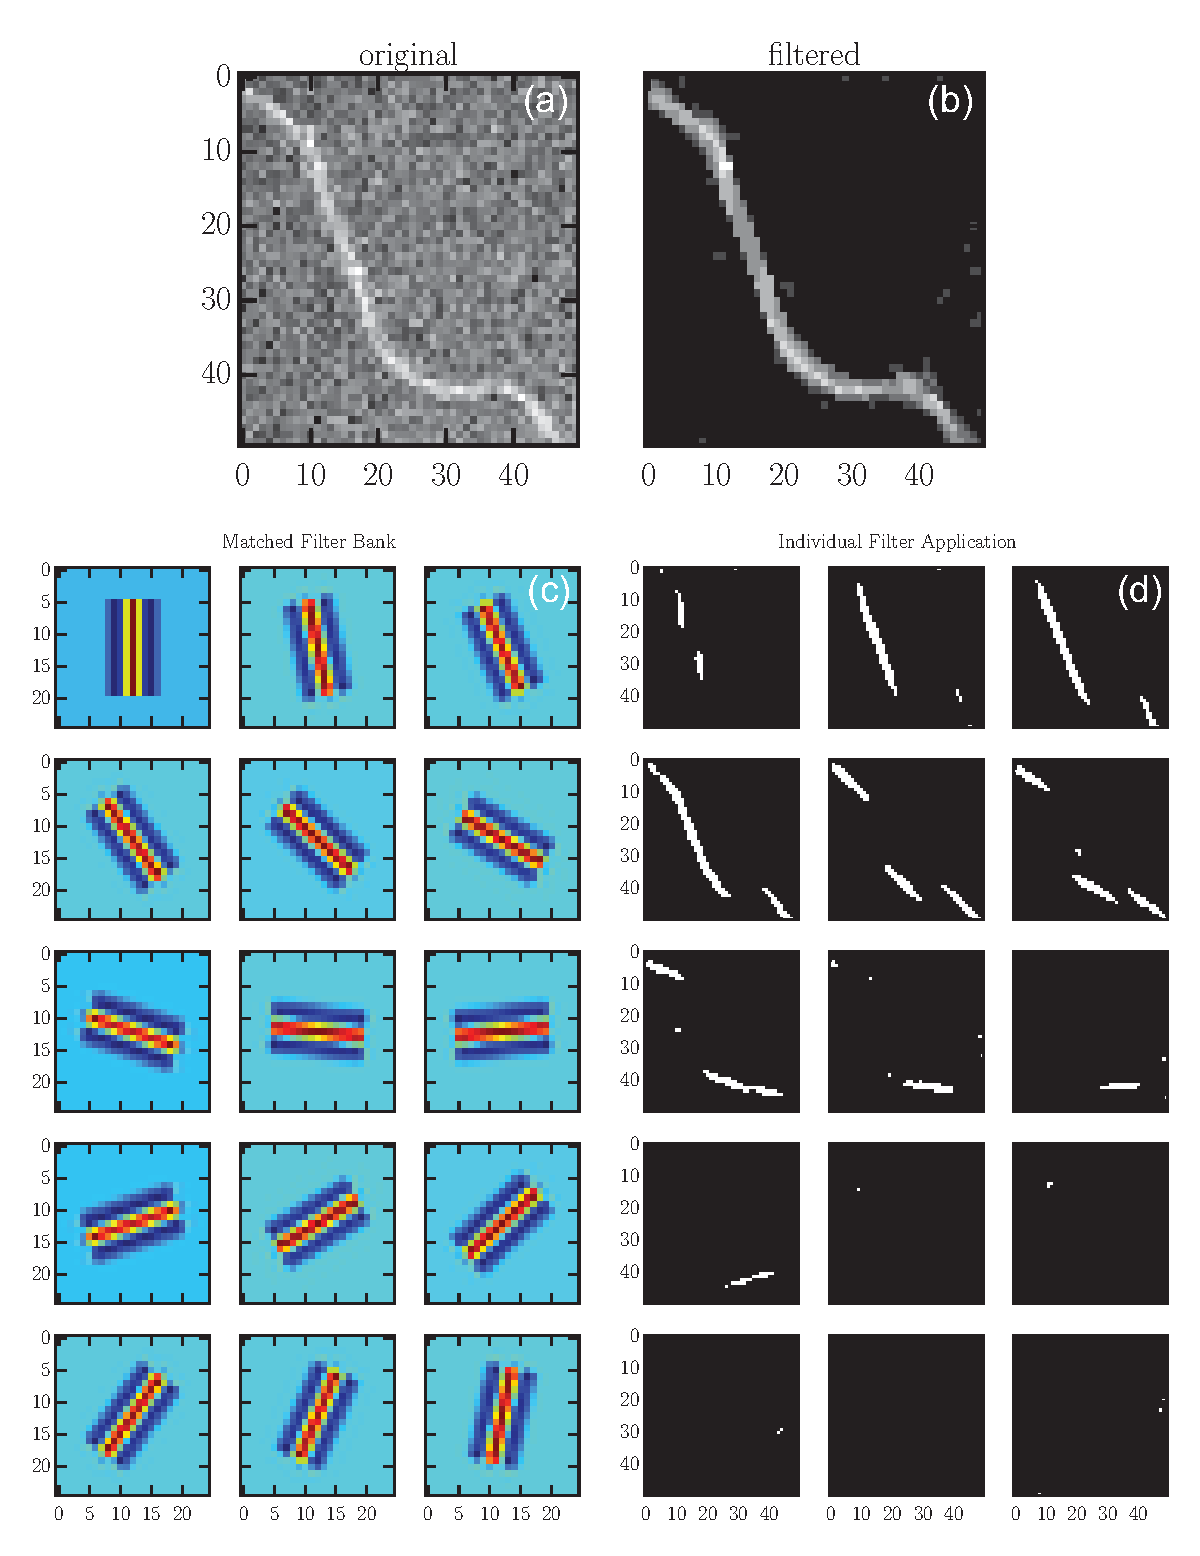
\includegraphics[width = 0.8\textwidth]{chapter3/filter_bank_results.eps}
	\caption{a) Original image. b) Final filtered image, which is the sum of the binary images in (d). c) The rotated kernels that form the full matched filter bank. d) Each rotated kernel applied to an image in (a).}
	\label{fig:filter_bank_results}
\end{figure}

After each kernel has been separately convolved with the original image, and the threshold applied, those binary images are added together to produce the final filtered image. Figures \ref{fig:filter_bank_results}a and b show the original and filtered nanotube images. 

In building this filter, many parameters had to be optimized simultaneously and compared by eye. Due to the large parameter space, the matched filters were optimized by iteratively varying a single parameter and choosing the best result. This process is illustrated in Figure \ref{fig:filter_parameter_test}.

\begin{figure}
	\centering
	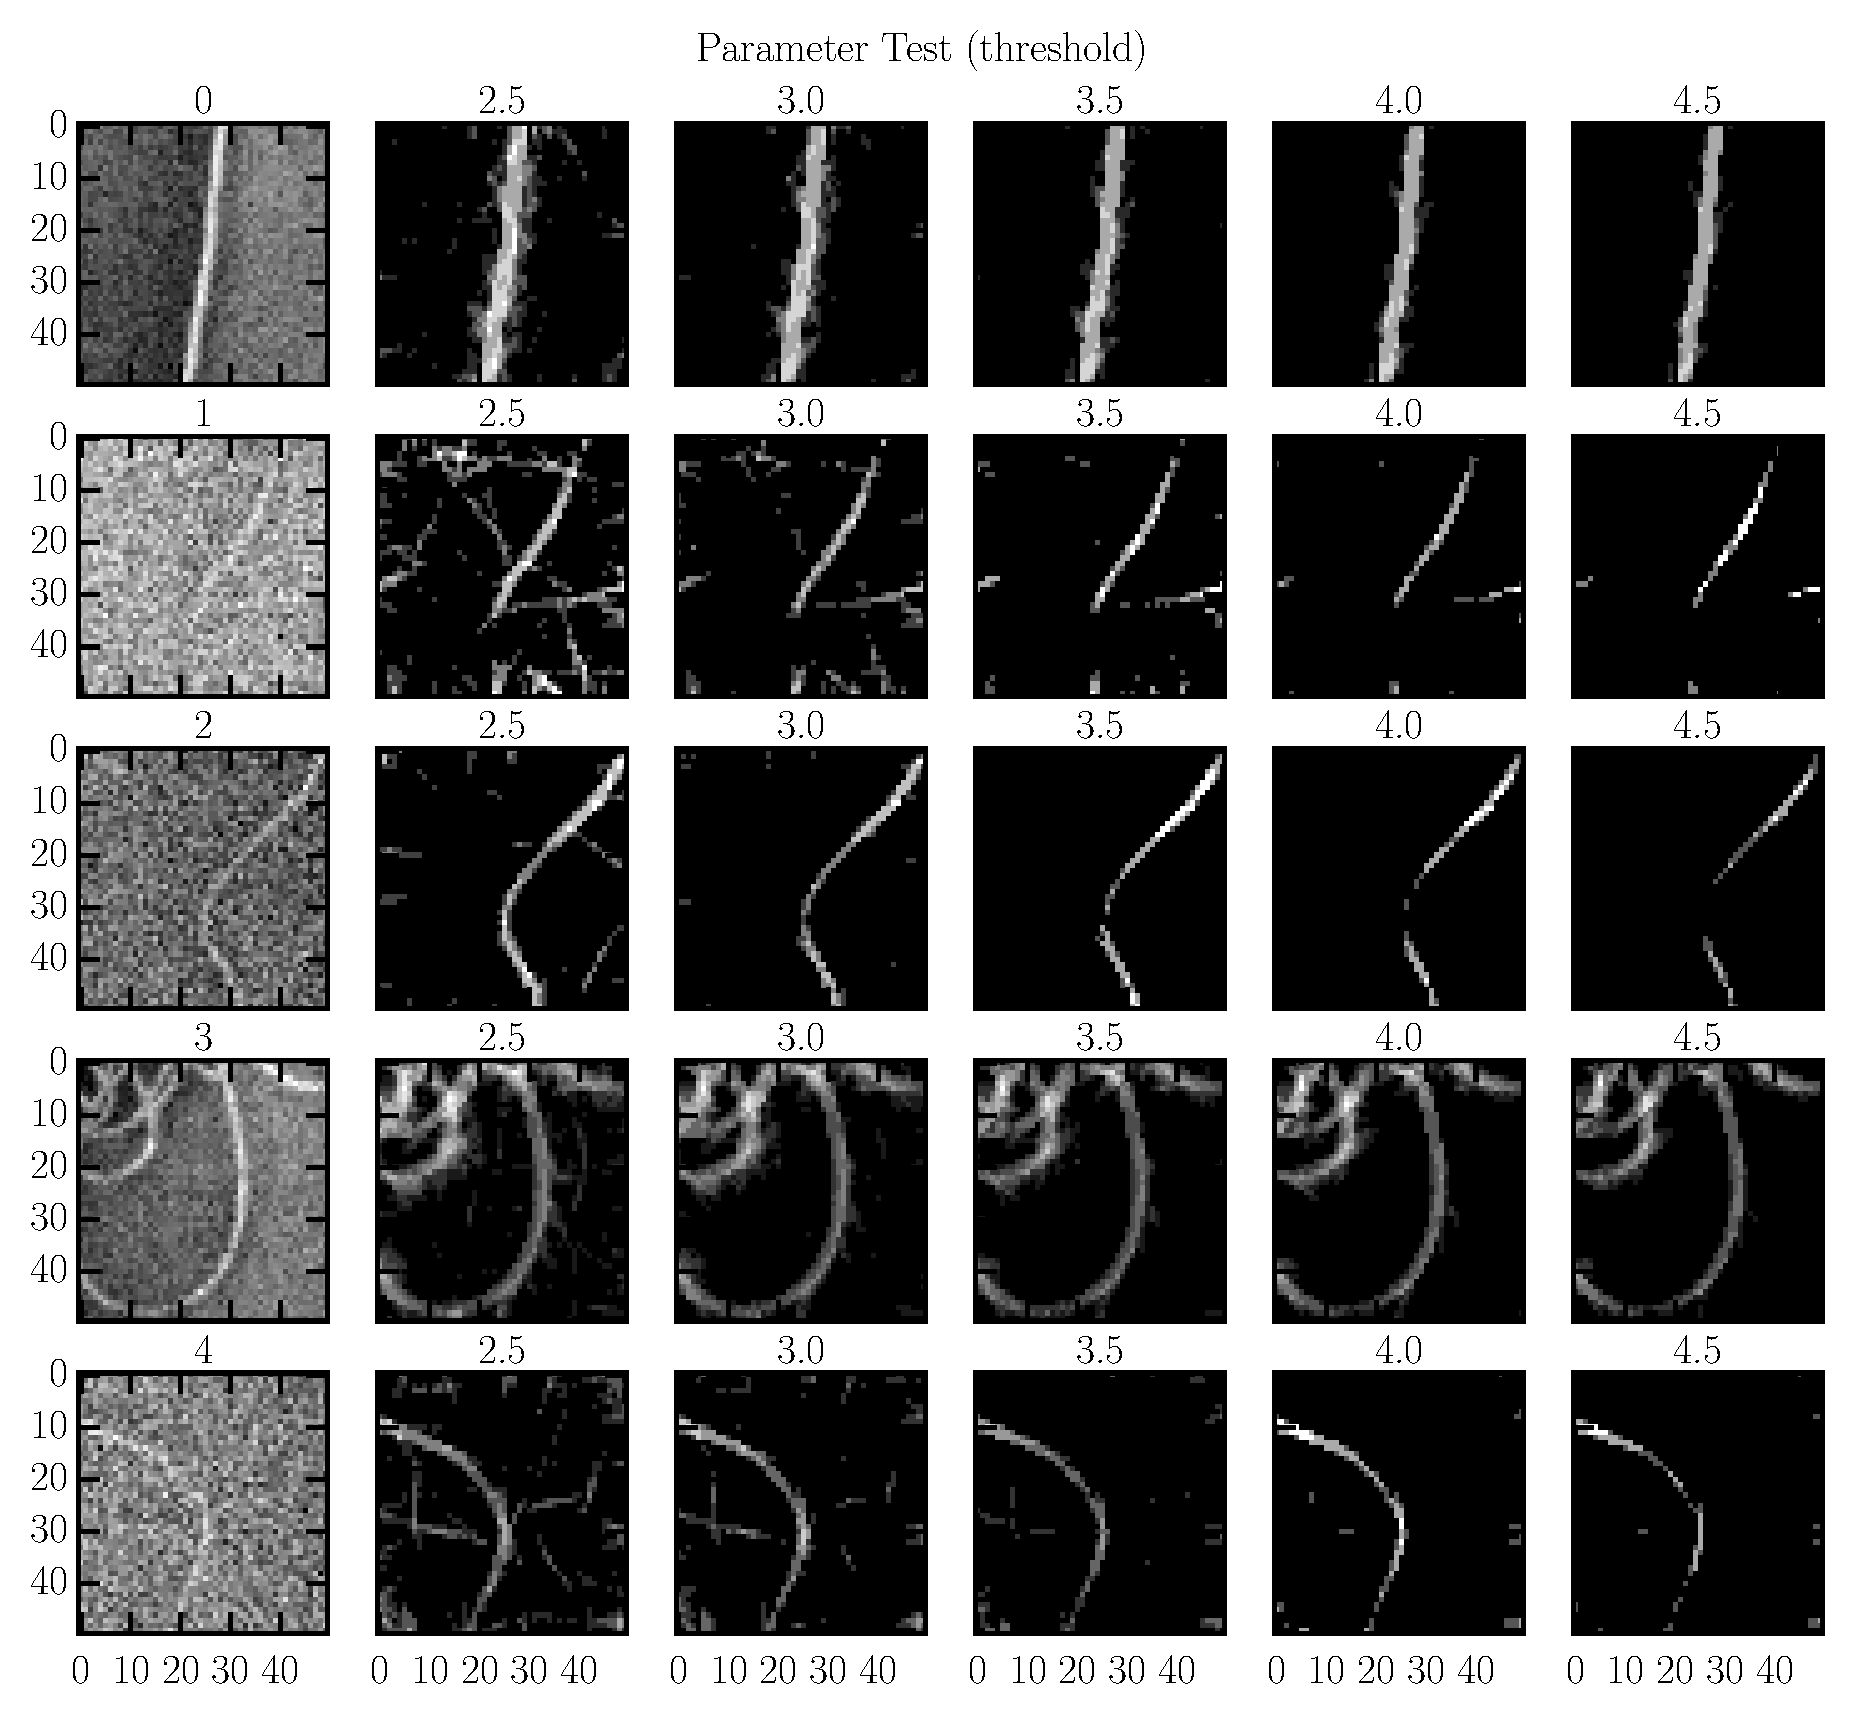
\includegraphics[width = 0.7\textwidth]{chapter3/filter_parameter_test.pdf}
	\caption{Optimization of the matched filter bank threshold value.}
	\label{fig:filter_parameter_test}
\end{figure}

The results of this optimization are seen in Table \ref{table:filter_parameters}. The optimized values for $k$ and $L$ were very close to those obtained from the original analysis of extracted nanotube profiles. Note that $A$ and $threshold$ are not independent values and $A$ remained fixed for this optimization procedure. 

It is also important to note that the length scale for these parameters is in pixels $(px)$. The randomly selected SEM images that were used for this analysis were not all take at the same magnification level. However, the average magnification was $850\times$ giving a pixel size of $\sim$\SI{140}{\nano\meter}

\begin{table}
	\centering
	\caption{Matched Filter Bank Parameters}
	%\hfill \\
    \begin{tabular}{| r | p{60mm} | l |}
    	\hline
    	\textbf{Parameter} & \textbf{Description} & \textbf{Optimized Value}  \\ \hline
    	k & inverse length scale for $sinc$ fit &  $1.75 px^{-1}$ \\ \hline
    	A & height of $sinc$ function in $K(x,y)$ &  $10$ \\ \hline
    	L & length of straight nanotube sections to search for &  $16 px$ \\ \hline
    	N & size of the kernel matrix &  $25$ \\ \hline
        R & number of kernels in the filter & $15$ \\ \hline
        threshold & cutoff value for thresholding images convolved with filter kernels & $3.6$ \\ \hline
    \end{tabular}
    \label{table:filter_parameters}
\end{table}

Finally, the filter was tested with the original set of full device SEM images. A selection of the results can be seen in Figure \ref{fig:full_image_filter}. It is clear from this set of images that the filter has the desired result. Nanotubes are much more clearly visible and the background is almost completely removed. Because the filter is very similar in its construction to common edge detection algorithms, it also leaves features at the edges of the optical lithography leads and markers defined on the substrate before nanotube growth. This actually works well, since those features are used to align the SEM images for additional electron beam lithography steps. 

\begin{figure}
	\centering
	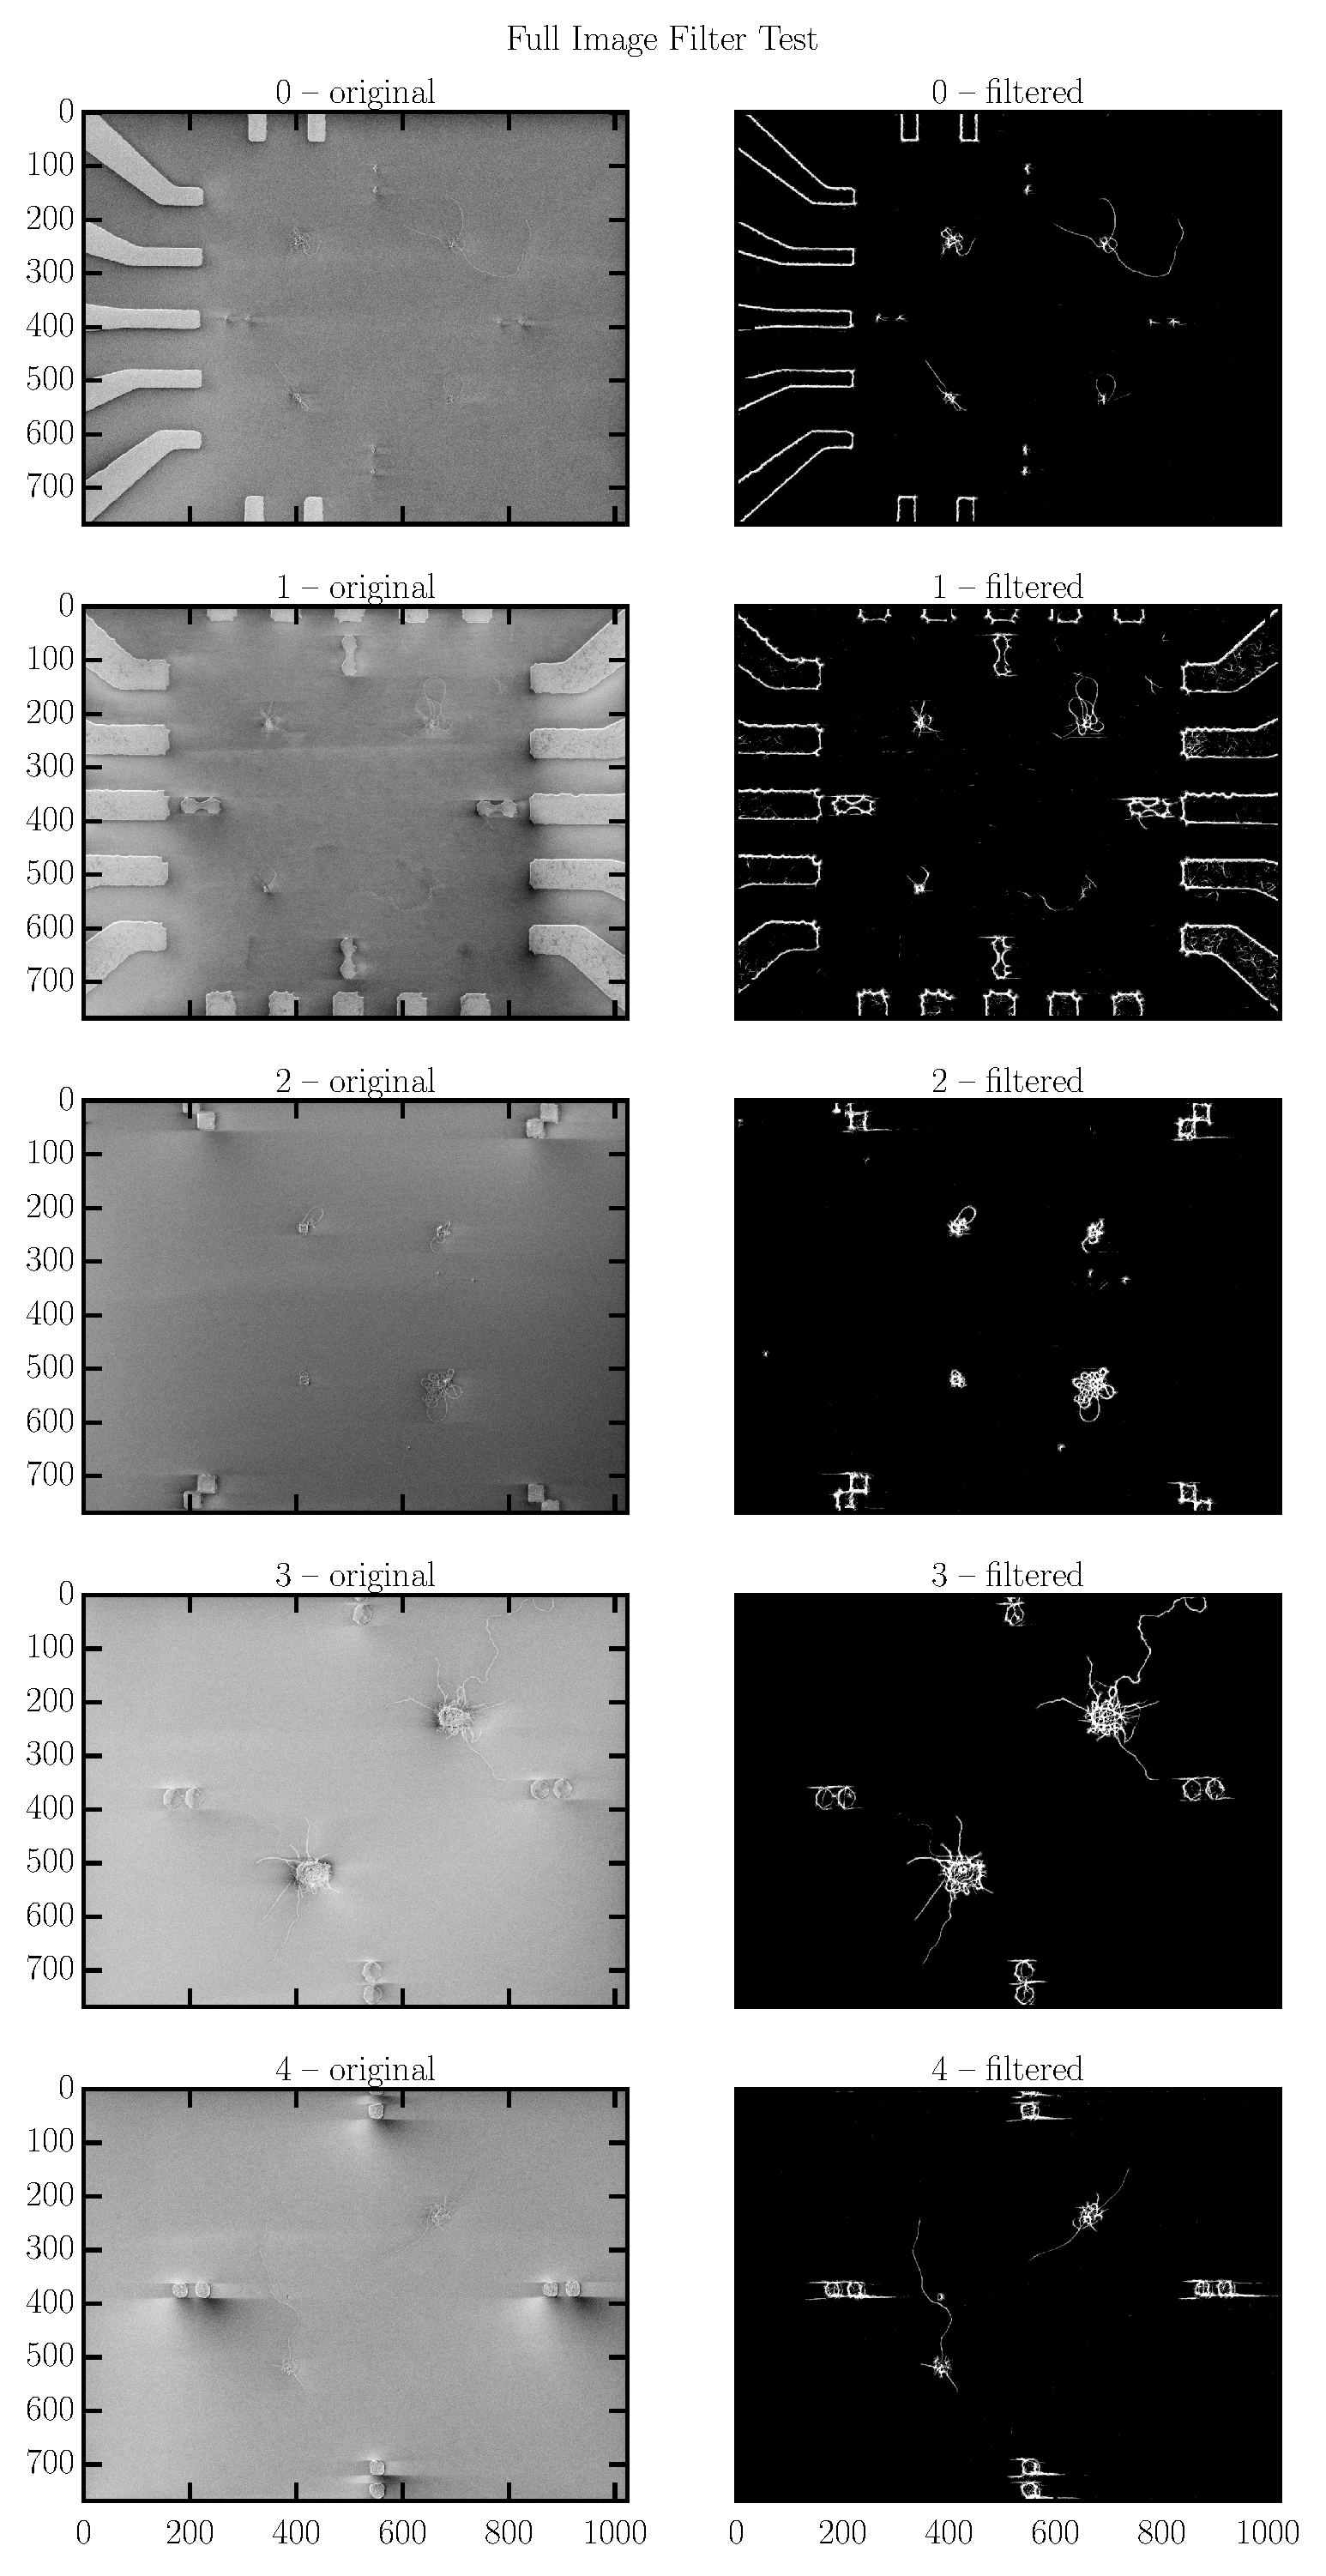
\includegraphics[width = 1.0\textwidth]{chapter3/full_image_filter_test.pdf}
	\caption{Two examples applying the matched filter bank to full SEM images of as-grown carbon nanotubes.}
	\label{fig:full_image_filter}
\end{figure} % growth of CNT, placement on substrate, imaging
\chapter{Metallic Contacts to Carbon Nanotubes}
\label{sec:contacts}
\chaptermark{Contacts to CNTs}

Chapter will contain: an explanation of the nature of metal-nanotube interfaces, statistics on metals tested, thin film deposition methods, and lithography methods. opinions will be backed up with a lot of histograms, contact resistance data, and device images. It's not the most exciting chapter, but it is what I spent a great deal of time thinking about over the past two years. %barrier info, statistics on lithography/deposition methods
\chapter{Quantum Dots with Ferromagnetic Leads}
\label{sec:FMCNTQD}
\chaptermark{Ferromagnetic CNTQD}

Of the many samples discussed in Chapter \ref{chap:contacts}, seven F-CNT-F devices were measured at low temperatures. Details, including room temperature resistance, can be seen in Table \ref{table:rt_fm_devices}.

\begin{table}
    \centering
    \footnotesize
    \begin{tabular}{ r | c | c c c}
        Sample & Leads & Material & Deposition Method & R($T=300K$) \\ \hline
        SCF72 & 17-19 & Co & sputter & \SI{65}{\kilo\ohm} \\
        SCF72 & 21-23 & Co & sputter & \SI{76}{\kilo\ohm}\\
        SCF75 & 21-23 & Co & sputter & \SI{280}{\kilo\ohm}\\
        SCF75 & 15-16 & Co & sputter & \SI{30}{\kilo\ohm}\\
        SCF96 & 9-12  & Co & electron beam evaporation & \SI{200}{\kilo\ohm}\\
        SCF96 & 16-17 & Co & electron beam evaporation & \SI{400}{\kilo\ohm}\\
        SCF98 & 11-12 & Co & electron beam evaporation & \SI{120}{\kilo\ohm}\\
        \label{table:rt_fm_devices}  
    \end{tabular}
    \caption{Details of measured F-CNT-F devices}
\end{table}

Each of these samples was measured at 4K, with the exception of SCF98 (11-12) which was measured at 150mK. Figure \ref{fig:all_FM_QD} shows Coulomb diamond plots for each of the samples. These were used to calculate the quantum dot properties seen in Table \ref{table:cold_fm_devices}

\begin{table}
    \centering
    \footnotesize
    \begin{tabular}{ r | r | c c c c c c c}
        Sample & Leads & $\Delta \mu (meV)$ & $\Delta E (meV)$ & $\frac{e^2}{2C} (meV)$ & $L_{measured} (nm)$ & $L_{design}$ (nm) & $C_{\Sigma} (aF)$ & $\alpha_{G}$ \\ \hline
        SCF72 & 23-21 & 8  & x   & x    & 175 & 300 & x  & 0.080 \\ 
        SCF72 & 17-19 & 8  & 1.8 & 6.2  & 280 & 300 & 13 & 0.072 \\
        SCF75 & 21-23 & 15 & 4.5 & 11.5 & 110 & 300 & 7  & 0.075 \\
        SCF75 & 15-16 & 12 & 3.5 & 8.5  & 140 & 300 & 9  & 0.110 \\
        SCF96 & 9-12  & 30 & 4.0 & 26.0 & 125 & 300 & 3  & 0.011 \\
        SCF96 & 16-17 & 22 & 2.0 & 20.0 & 250 & 300 & 4  & 0.006 \\
        SCF98 & 11-12 & 7  & 1.8 & 5.2  & 280 & 300 & 15 & 0.005 \\
        \label{table:cold_fm_devices}  
    \end{tabular}
    \caption{Low temperature characteristics of F-CNT-F quantum dots}
\end{table}

\begin{figure}
    \centering
    \includegraphics[width=1.0\textwidth]{fmdots/all_fm_dots.png}
    \caption{Conductance as a function of $V_{bias}$ and $V_{gate}$ for all measured ferromagnetic quantum dots.}
    \label{fig:all_FM_QD}
\end{figure}

The lever arm, $\alpha_{G}$, defined as $\alpha_{G} = C_G/C_{\Sigma}$ and is used to convert gate voltages to energies, $U_{gate} = \alpha_{G}eV_{gate}$ \cite{Ihn2004}. It can be calculated based on the geometry of the Coulomb diamonds, as illustrated in Figure \ref{fig:alpha_calc} and characterizes the coupling regime for each device. Looking at the lever arm values, the electron beam evaporated samples are in a much weaker coupling regime than the sputtered samples. All other aspects of the fabrication were the same over all four chips. 

\begin{figure}
    \centering
    \includegraphics[width=0.6\textwidth]{fmdots/alpha_calc.pdf}
    \caption{Calculating the lever arm using Coulomb diamond geometry.}
    \label{fig:alpha_calc}
\end{figure}

\section{Tunneling Magnetoresistance}
\label{sec:TMR}

Tunneling magnetoresistance is a change in resistance measured across a ferromagnet/insulator/ferromagnet structure as a function of magnetic field. The spin transport through such an interface can be made tunable by replacing the insulator with a carbon nanotube quantum dot. Exchange coupling with the ferromagnetic leads will split the spin degeneracy of the quantum dot, making it possible to tune the magnitude and even the sign of the tunneling magnetoresistance \cite{Tsymbal2003, Sahoo2005, Thamankar2006}.

The magnetization of the carbon nanotube contacts is dominated by their shape anisotropy. This is typical for polycrystaline sputtered and electron beam evaporated films, such as the ones used in these samples. By patterning the contacts with different widths, they have different coercive fields at which the magnetization will be flipped as an external, parallel magnetic field is varied. A schematic of the situation can be seen in Figure \ref{fig:spin_valve}.

\begin{figure}
    \centering
    \includegraphics[width=0.9\textwidth]{fmdots/TMR.pdf}
    \caption{Top: A diagram of the magnetization of the ferromagnetic nanotube contacts corresponding to the data shown in the lower plot. Bottom: TMR signal measured through a carbon nanotube quantum dot.}
    \label{fig:spin_valve}
\end{figure}

\subsection{Results}

Of the ferromagnetic devices measured, only sample SCF72 showed clear tunneling magnetoresistance behavior. Refer to the previous section for details on that sample. In the other devices the effect was overwhelmed by random telegraph noise in the data, which can look a lot like false TMR signals, or metal/nanotube barriers had impurities causing spin-flip events that destroyed the TMR effect.

\begin{figure}
    \centering
    \includegraphics[width=0.9\textwidth]{fmdots/scf72_17-19_TMR_4K.pdf}
    \caption{Tunneling magnetoresistance measurements taken on device SCF72 (17-19) at $V_{gate} = 0V$. The plots show data for $V_{bias} = 5mV$ (left) and $V_{bias} = 10mV$ (right).}
    \label{fig:TMR_real}
\end{figure}

In the simplest mode, tunneling magnetoresistance is defined as:

\begin{align}
    TMR &\equiv \frac{G_P - G_{AP}}{G_P + G_{AP}} = \frac{R_{AP} - R_{P}}{R_P + R_{AP}} \\
    TMR &= P_L P_R \label{eq:basic_tmr}
\end{align}

Where $P_{L(R)}$ are the spin polarizations at the Fermi level for the left and right nanotube contacts \cite{Maekawa1982}. This polarization is defined as:

\begin{equation}
    P_{L(R)} = \frac{\rho^{L(R)}_{+} - \rho^{L(R)}_{-}}{\rho^{L(R)}_{+} + \rho^{L(R)}_{-}}
\end{equation}

And $\rho^{L(R)}_{+(-)}$ are the tunneling density of states for the majority (minority) spins at the Fermi level. With all of this one expects that $P_{L(R)}$ will be positive, thus the TMR signal will be positive.

In the data shown in Figure \ref{fig:TMR_real}, the TMR signal is measured to be about -6.0\% and -0.8\% in the left and right plots, respectively. Additionally, the coercive fields for the two cobalt contacts are 40mT and 60mT. These coercive field measurements are consistent with the predicted values for narrow cobalt wires.

The TMR signal has a magnitude consistent with the predicted values \cite{Maekawa1982}, but with the opposite sign. This change in sign of the TMR signal has previously been explained by a resonant tunneling model with asymmetric coupling of the left and right contacts to the nanotube. The model as described here is taken from \cite{Tsymbal2003}.

First the conductance through the quantum dot can be written as:

\begin{equation}
\label{eq:tunnel_conductance}
    G(E) = \frac{4e^2}{h} \frac{\Gamma_L \Gamma_R}{(E-E_i)^2 + (\Gamma_L + \Gamma_R)^2}
\end{equation}

Here, $\Gamma_{L(R)}$ are the tunneling rates on/off the quantum dot from the left(right) ferromagnetic contacts. These tunneling rates can be thought of as being proportional to the density of states of the on the leads. $E_i$ is the energy of the quantum dot level nearest to the Fermi level of the leads, $E$. 

When the quantum dot is tuned off resonance, $|E-E_i| \gg \Gamma_L + \Gamma_R$, the TMR signal is predicted by Equation \ref{eq:basic_tmr}. Near a resonant level, $E \sim E_i$ the situation is quite different. Considering the limit where $\Gamma_L \gg \Gamma_R$, Equation \ref{eq:tunnel_conductance} simplifies to $G \sim \frac{\Gamma_R}{\Gamma_L}$. The conductance is now inversely proportional to the density of states on one of the leads, which leads to a sign inversion of the TMR signal.

\begin{equation}
\label{eq:sign_inversion}
    TMR = -P_L P_R
\end{equation}

By using a carbon nanotube quantum dot, the TMR signal can be modulated by tunning the resonant energy level $E_i$ with the gate voltage. Additionally, the magnitude can be modulated because the levels on the quantum dot are spin non-degenerate due to the exchange coupling field introduced by the magnetic leads. This effect has been observed previously in carbon nanotube quantum dots \cite{Sahoo2005, Thamankar2006}. 

In sample SCF72, the TMR signal was only significant in a narrow range of gate voltages near $V_{gate}=0V$, as shown in Figure \ref{fig:TMR_real}. Looking at the conductance data as a function of the gate voltage in Figure \ref{fig:TMR_gate}, it is clear that at $V_{gate}=0V$ there is a quantum dot level $E_i$ resonant with the Fermi level on the leads. Therefore, the observed negative TMR signal makes sense in terms of the model described.

\begin{figure}
    \centering
    \includegraphics[width=0.5\textwidth]{fmdots/scf72_17-19_gateswp-for-TMR.pdf}
    \caption{Conductance as a function of $V_{gate}$ for sample SCF72. Note the conductance peak at $V_{gate}=0V$.}
    \label{fig:TMR_gate}
\end{figure}

\section{Negative Differential Conductance in Coulomb Blockade Regime}

Negative differential conductance resulting from spin blockade has been observed in two devices measured. The data is presented in Figure \ref{fig:negative_differential_conductance}. This section will attempt to explain the NDC feature in terms of two models. Neither model is dependent on the fact that the leads are ferromagnetic. No TMR was measured in these devices. An exchange interaction still exists between the ferromagnets and quantum dot levels to lift the spin degeneracy. Additionally, the tunnel barriers between the leads and sample should be spin dependent.

\begin{figure}
    \centering
    \includegraphics[width=0.9\textwidth]{fmdots/scf75_scf96_ndc.pdf}
    \caption{Conductance as a function of $V_{bias}$ and $V_{gate}$ in samples SCF75 (left) and SCF96 (right). Note the differential conductance peaks in dark blue running parallel to the diamond edges in each sample.}
    \label{fig:negative_differential_conductance}
\end{figure}

\subsection{Spin Blockade in a Double Quantum Dot}
\label{sec:dqd_model}

Defects or impurities along the length of a nanotube quantum dot can form small tunnel barriers that interrupt electron transport through the dot \cite{McEuen1999, Bockrath2001}. These tunnel barriers define multiple quantum dots between the fabricated leads on the sample. This is a commonly observed problem in substrate grown carbon nanotubes. Other work has exploited similar defects to form tunable double quantum dots \cite{Mason2004, Jorgensen2007}.

With careful analysis, the formation of multiple quantum dots in series can lead to interesting physical situations not observed in single quantum dot devices. Two quantum dots formed in series by a defect or impurity have much lower tunnel barriers and stronger coupling than double quantum dots formed by the patterning of local gates. Thanks to this strong coupling between dots, spin interactions can be observed that are not seen in as-fabricated double quantum dot structures. In 2008, Buitelaar et al. used this idea to measure Pauli spin blockade in a carbon nanotube double quantum dot \cite{Buitelaar2008}. The model relies on the formation of a double quantum dot by an impurity.

Table \ref{table:cold_fm_devices} shows samples SCF75 (15-16) and SCF96 (9-12) have calculated lengths of 140nm and 110nm, respectively. Comparing this to the 300nm spacing between cobalt leads suggests that the quantum dot being measured in each case is defined by defects along the nanotube. This is supported by the gate measurements that show no clear periodicity in Figure \ref{fig:scf75_scf96_gates}. One final piece of evidence for a double quantum dot is the suppressed conductance in the SCF75 levels around $V_{gate}=5.9V$, this can be attributed to one dot being off resonance while the other is not. This feature also suggests the back gate coupling for each quantum dot is quite different, thus the gate dependent features are dominated by a single dot in the series.

\begin{figure}
    \centering
    \includegraphics[width=0.9\textwidth]{fmdots/scf75_scf96_gates.pdf}
    \caption{Current as a function of $V_{gate}$ in samples SCF75 (top) and SCF96 (bottom). No clear periodicity is visible in either measurement implying disorder along the nanotube.}
    \label{fig:scf75_scf96_gates}
\end{figure}

Figure \ref{fig:buitelaar_levels} illustrates the basic principles of the proposed model. It based on a hybridization between levels in the two strongly coupled quantum dots. Spin blockade then comes from a forbidden transition between the (1,1) spin triplet state and the (0,2) spin singlet state.

\begin{figure}
    \centering
    \includegraphics[width=1.0\textwidth]{fmdots/buitelaar_levels.png}
    \caption{Figure adapted from \cite{Buitelaar2008}. (a) Double quantum dot levels. Numbering refers to the occupation of (QDA,QDB). $\delta \epsilon$ is the splitting between single particle energy levels. $U$ and $U'$ are the charging energies. (b) With strong coupling the (1,1) and (0,2) states hybridize to form bonding and anti-bonding orbitals $S_1$ and $S_2$ different from the triplet state $T$. (c) At negative bias the (1,1) to (0,2) transition is forbidden by spin blockade as the (0,2) must be a spin singlet. (d) The transition is allowed in the reverse bias situation.}
    \label{fig:buitelaar_levels}
\end{figure}

Figure \ref{fig:dqd_model_compare} shows the data from SCF75 alongside the simulation from Buitelaar et al. Note the similarities in the negative differential conductance peak in the data and simulation. The simulation was run for a device 300nm in length with a defect in the center, giving two dots of size 150nm, consistent with Table \ref{table:cold_fm_devices}. Using $\alpha_G = 0.11$ , gives an energy spacing between the two zero bias conductance peaks of 15.4meV, which agrees well with the simulation parameters. The situation is identical for SCF96, with the exception of the gate coupling.

\begin{figure}
    \centering
    \includegraphics[width=0.9\textwidth]{fmdots/dqd_model_compare.png}
    \caption{A comparison of the SCF75 negative differential conductance data (a) with double quantum dot data (b) and simulations (c) from Reference \cite{Buitelaar2008}.}
    \label{fig:dqd_model_compare}
\end{figure}

\subsection{NDC from Spin Selection Rules}
\label{sec:single_dot_model}

The negative differential conductance peaks seen in Figure \ref{fig:negative_differential_conductance} may be explained by a simpler, single dot model, but not necessarily captured by the constant interaction model discussed in Section \ref{sec:constant_interaction_model}. As electrons fill the quantum dot, they are not only subject to charge interactions, but also spin interactions. Each quantum dot occupation number has many possible collective spin states. Figure \ref{fig:spin_states} tabulates some of these states for low occupation numbers, calculated from Clebsh-Gordan coefficients \cite{Weinmann1994} .

\begin{figure}
    \centering
    \includegraphics[width=0.8\textwidth]{fmdots/spin_states.png}
    \caption{Table tabulating possible occupation numbers, spin states, and relevant energy level splittings for low occupation number quantum dots as calculated by Weinmann et al. \cite{Weinmann1994}.}
    \label{fig:spin_states}
\end{figure}

This means that there are spin selection rules that can determine the lifetime of a given quantum dot state. Consider, for example, a state with occupation number $n$ and maximal spin, $S=n/2$. This is possible when transport occurs though excited states in a 1D quantum dot. The $S=n/2$ state must transition to a nearby state ($n-1$, $S'=(n-1)/2$). Since the spin can only change by -1/2, not $\pm$1/2, $S=n/2$ is a relatively long lived state. When this state is brought into resonance with the Fermi level on the leads, the current through the dot is reduced, leading to a negative differential conductance peak. Figure \ref{fig:weinmann_compare} compares qualitatively a simulation of this effect with the data from SCF96 \cite{Weinmann1995}. 

\begin{figure}
    \centering
    \includegraphics[width=0.8\textwidth]{fmdots/weinmann_compare.pdf}
    \caption{A comparison between simulated transport through a quantum dot with spin selection rules and data from SCF75. The simulation is taken from Weinmann et al. \cite{Weinmann1995}. Simulation data shows regions of negative differential conductance as bright white lines. Data on the right shows regions of negative differential conductance in dark blue.}
    \label{fig:weinmann_compare}
\end{figure}

A similar effect can explain the missing ground state transitions seen in the data for SCF96. If the spin ground states for two adjacent quantum dot occupation numbers differ by more than $1/2$ the conductance peak is missing from the stability diagram.

These calculations assume spin degenerate levels and symmetric coupling to normal metal leads. Without a direct measure of the exchange coupling in ferromagnetically contacted nanotubes, it is unclear if the first criterion is met. The second condition is clearly not met, but it is not required, just a simplification. It is easy to imagine that these types of spin selection rules will be exaggerated further by reducing one spin population and introducing spin dependent tunnel barriers. See Figure \ref{fig:scf72_info}(a) for a model of such a quantum dot.

\section{Spin Selection Rules with Applied Magnetic Field}
\label{sec:spin_selection_field}

Additional data supporting the suppression of conductance peaks in ferromagnetic quantum dots due to spin selection rules is observed in sample SCF72. This dot has been used throughout this thesis as the canonical example of a Coulomb blockade measurement. It shows regular oscillations in the gate, suggesting a single dot with levels that are not split by exchange coupling or disorder. An energy level diagram of the quantum dot, tunnel barriers, and the data can be seen in Figure \ref{fig:scf72_info}(a). 

\begin{figure}
    \centering
    \includegraphics[width=1.0\textwidth]{fmdots/scf72_info.pdf}
    \caption{(a) Energy level diagram for an F-CNT-F quantum dot. The two barrier colors represent the two spin dependent tunnel barrier heights for spin up and spin down electrons. Blue and red arrows illustrate the different tunneling rates for up and down spins. (b) SCF72 conductance at $B=0$. (c) SCF72 conductance at $B=4T$.}
    \label{fig:scf72_info}
\end{figure}

Figure \ref{fig:scf72_spin_selection} shows Coulomb diamond data for SCF72 at $B=0$T and -4T; suppressed conductance levels are marked with dashed lines. Conductance peaks that mark ground state transitions between different dot occupation numbers (those that cross $V_{bias}=0mV$) are suppressed as the applied field is increased. This can be understood in light of the discussion in Section \ref{sec:single_dot_model}. Applying a strong magnetic field changes the spin ground state to one in which adjacent occupation numbers have spin levels differing by more than $\Delta S = 1/2$ as predicted by the constant interaction model. Looking at the excited states, it is clear that there is a similar change in which excited states are suppressed based on the change in lowest energy spin states.

\begin{figure}
    \centering
    \includegraphics[width=1.0\textwidth]{fmdots/scf72_spin_selection.pdf}
    \caption{Conductance as a function of $V_{gate}$ ang $V_{bias}$ for sample SCF72 at $B=0$T (left) and -4T (right). Solid lines trace conductance peaks. Dashed lines trace suppressed peaks.}
    \label{fig:scf72_spin_selection}
\end{figure}

The Zeeman splitting can be measured by measuring the change in excited state energies as the magnitude of the field is increased. At zero field, excited states are separated by $\Delta E = 1.8$meV. In a field of -4T, the levels are separated by $\Delta E = 2.0meV$. This certainly shows that the excited states are spin dependent. It is also consistent with the Zeeman splitting of $g \mu_B (-4T) =-0.25 g$meV. The $g$-factor in carbon nanotubes is measured to be approximately 2 \cite{Cobden1998}, but has been found to be tunable in some devices \cite{Lai2014}. This measurement really shows that the excited state levels are not spin degenerate. If the levels were, the spacing would not only change, but single excited state levels would be seen to split into two. This implies a non-zero exchange coupling field in the nanotube from the ferromagnetic leads.

\subsection{Results and Discussion}

Effects of spin selection rules have potentially been observed in three samples. At least one of these samples, SCF72, is proven to be a clean, single quantum dot. This suggests that spin selection rules beyond the constant interaction model might be a better explanation for suppressed and negative differential conductance features though these quantum dots. Additional work must be done in modeling transport though a F-CNT-F dot to confirm that the features observed here can be accurately fit with this model. However, given the rich nature of spin physics in ferromagnetic quantum dots this is a much more attractive model with which to compare the data.

\section{Spectroscopy of a Magnetic Impurity}
\label{sec:imurity_tunneling}

It is possbile, through transport spectroscopy, to identify impurities near a quantum dot and infer some of their characteristics. Sample SCF96 shows such impurity levels. The transport through the impurity was found to be tunable by varying the gate voltage and external magnetic field. The data is show in Figure \ref{fig:resonant_tunneling}

\begin{figure}
    \centering
    \includegraphics[width=0.9\textwidth]{fmdots/scf96_resonant_tunneling_conductance.pdf}
    \caption{Top: Conductance as a function of $V_{bias}$ and $V_{gate}$ in zero field. Bottom: Conductance measured over the same portion of the quantum dot spectrum in a 2T magnetic field.}
    \label{fig:resonant_tunneling}
\end{figure}

Looking at the data it is clear that their are positive and negative differential conductance peaks that cut through the Coulomb blockaded regions of the conductance plot at positive bias in zero magnetic field. Both the positive and negative conductance peaks are suppressed at 2T.

\subsection{Characteristic Size and Level Spacing}

Figure \ref{fig:resonance_cuts} shows cuts through each of the three Coulomb diamonds where the resonance peaks are observed. Looking at plots at constant gate voltage, it is clear that the resonances have both positive and negative peaks in the conductance, with some background conductance superimposed due to the conductance through the nanotube quantum dot levels.

\begin{figure}
    \centering
    \includegraphics[width=0.9\textwidth]{fmdots/scf96_resonant_tunneling_cuts.pdf}
    \caption{Top: Conductance as a function of $V_{bias}$ and $V_{gate}$ in zero field. Bottom: Conductance measured over the same portion of the quantum dot spectrum in a 2T magnetic field.}
    \label{fig:resonance_cuts}
\end{figure}

From the data in Figure \ref{fig:resonance_cuts} it is possible to derive the relevant energy scales of the impurity level. Positive and negative conductance peaks are split by 2meV. Adjacent positive peaks are separated by 5meV. This suggests that the impurity has at least 3 energy levels that are separated by 5meV. These three levels are spin split by 2meV, most likely because the impurity is itself ferromagnetic.

%The negative differential conductance can be understood in terms of spin blockade. The impurity levels are split such that levels with the same spin polarization as the nearest ferromagnetic contact are lower energy than those with opposite polarization. When a level with spin polarized anti-parallel to the lead is in resonance, current is suppressed through the impurity. This leads to a decrease in the conductance. In regions where transport through the nanotube is suppressed by the Coulomb blockade, the total measured conductance is negative.

The charging energy for the impurity can be measured using the lever arm calculated in Table \ref{table:cold_fm_devices}. Resonant tunneling through the impurity is observed for gate voltages between 10 and 20V. With the lever arm of $\alpha_G = 0.006$ the charging energy can be estimated to be roughly 100meV, which corresponds to a capacitance of about $C_{\Sigma} = 0.8$aF. 

The most likely origin of this impurity is a piece of magnetic contamination. The size of the impurity can be estimated in two ways. First, it can be estimated using the capacitance calculated above. Considering the impurity as a spherical metal shell gives $C_{\Sigma} \sim 4\pi \epsilon_0 r = 0.8$aF. With that, the radius is calculated to be $r = 7$nm. The size can also be estimated quantum mechanically from the level spacing, $\Delta E = 5$meV. Assuming the impurity is a 3D spherical well, the levels are $E_{n,l} = \frac{\hbar^2}{2ma^2}z_{n,l}^2$ where $z_{n,l}$ is the nth zero of the lth spherical Bessel function. For $l=0$, the level spacing is $\Delta E = \frac{\pi \hbar^2}{2mr^2}$. Using the measured value $\Delta E = 5meV$ gives an estimate for the radius of $r = 5$nm. These two estimates are in good agreement and suggest an origin for the impurity. A 10nm diameter magnetic particle on the substrate perfectly describes the iron nanoparticles used in the nanotube catalyst.

\subsection{Effects on CNT Quantum Dot Levels}

Additional interactions between the dot and impurity levels can be seen at negative bias in the 2T magnetic field data. This region is highlighted in Figure \ref{fig:scf96_ndc_impurity}.

\begin{figure}
    \centering
    \includegraphics[width=0.6\textwidth]{fmdots/scf96_ndc_impurity.pdf}
    \caption{Conductance as a function of $V_{bias}$ and $V_{gate}$ at $B=2T$ in sample SCF96. Note the difference in slope in the excited states of the two Coulomb diamonds seen at negative bias and the strong negative differential conductance.}
    \label{fig:scf96_ndc_impurity}
\end{figure}

There are two features to note in Figure \ref{fig:scf96_ndc_impurity}. The first is the change in slope of the two Coulomb diamonds seen at negative bias. This is a clear indication that the conductance measured is not due to a single quantum dot as described by the constant interaction model. Additionally, note the strong negative differential conductance seen in these same diamonds. Both of these features suggest some coupling between the levels on the nanotube quantum dot and in the nearby magnetic impurity. A similar coupling has been observed previously between a magnetic impurity and vibrational modes in a suspended nanotube \cite{Ganzhorn2013}. The exact nature of the coupling is not known, but it is likely that both of these observed features can be attributed to the presence of the magnetic impurity. The negative differential conductance in particular may fit with some existing models of hybridized levels in two quantum dots resulting negative differential conductance from spin blockade between the two dots as discussed in Section \ref{sec:dqd_model}. % describe results of FMCNTQD made in the ebeam evaporator that showed possibly interesting behavior. Basically, the group meeting talk from 2014
%\chapter{Carbon Nanotube Quantum Dot Tunnel Probe into Narrow Superconducting Wires}
\label{sec:CTNTAL}
\chaptermark{Tunnel Probe}

A carbon nanotube quantum dot is used as a tunnel probe into the density of states of a narrow aluminum wire placed on top of the quantum dot. The goal is to corroborate some of Tyler's Weber blockade results.

Many devices have been produced, some have worked, but the Al-CNT resistance has been too large to be useful. This device is currently the focus of my fabrication efforts. There is some data showing that the aluminum wire does not affect the behavior of the quantum dot underneath, and is itself superconducting with the expected $T_c$.   % use CNT QD as a tunnel probe into the density of states of a narrow aluminum wire
\chapter{Spin Transport in Tunable Ferromagnet/Superconductor Junction}
\label{sec:SCFM}
\chaptermark{F-CNT-S}

%%%%%%%%  Chapter starts below %%%%%%%%%%%

In 1971, Tedrow and Meservey made their famous measurement of the spin polarization in a ferromagnetic nickel thin film \cite{Tedrow1971}. This was done by creating a tunnel junction between the thin nickel film and a thin aluminum film. The density of states of the aluminum film was used as a probe into the spin polarization of the nickel film by measuring the conductance through the junction. Tedrow and Meservey later used this same technique to characterize a number of ferromagnetic materials \cite{Tedrow1973}

%The motivation for the work in this chapter was to make the same type of measurement using a carbon nanotube quantum dot as a spin tunable tunnel barrier between a ferromagnetic and superconducting lead. In doing so, the spin resolved density of states of each material could be inferred from the differential conductance through the quantum dot as a function of magnetic field.

The goal in this work was to replace the insulating barrier in the Meservey measurement with a carbon nanotube quantum dot. In doing so, it becomes possible to use the levels on the dot to further tune spin transport through the junction. Differential conductance measurements through such a F-CNT-S can be made to measure the ferromagnet polarization, exchange coupling in the carbon nanotube, and the spin-resolved density of states of the superconductor. The work presented in this chapter represents the first attempt to measure transport in this type of carbon nanotube quantum dot device.

\section{Background}

The results of the Tedrow and Meservey experiment can be described with a simple theory based on the density of states of the materials \cite{Meservey1994}. Figure \ref{fig:MT_explanation}(a) shows schematically the density of states on each side of the tunnel barrier in a non-zero magnetic field applied parallel to the thin films separated by an insulator. The ferromagnet has a larger number of spins aligned with its magnetization (and the applied field). In the superconducting film, the density of states is split due to Zeeman splitting in the applied magnetic field. The energy to add a spin up (aligned with the field) particle is lower than adding a spin down particle. 

\begin{figure}
    \centering
    \includegraphics[width=0.6\textwidth]{scfmdots/MT_explanation.pdf}
    \caption{(a) Energy diagram showing the density of states of each material in the F-I-S junction. Figure adapted from \cite{Moodera2010}. (b) Superconducting density of states with Zeeman splitting. (c) Spin-dependent kernel used to calculate the tunneling current. (d) Differential conductance as measured through the junction. Different spin-resolved peaks are labeled $\sigma_{1-4}$. Figures (b)-(d) are adapted from \cite{Meservey1994}.}
    \label{fig:MT_explanation}
\end{figure}

To begin, the tunneling current through a normal-insulator-superconductor junction can be written as follows:

\begin{equation}
    \label{eq:nis_junction}
    I \sim N_n \int N_s(E)[f(E+eV) - f(E)]dE
\end{equation}

Where $N_n$ is the normal metal density of states which is indenpendent of energy in 2D and $f(E)$ is the Fermi function. $E$ is the Fermi level in the system and V is the applied bias voltage. The superconducting density of states $N_s$ can be written in the BCS form \cite{Tinkham1996}:

\begin{equation}
    \label{eq:bcs_dos}
    N_s(E) = \begin{cases}
    N_n(E)E\frac{E}{sqrt{E^2 \Delta^2}}, & |E| \geq \Delta.\\
    0, & |E| < \Delta.
  \end{cases}
\end{equation}

Taking the derivative of Equation \ref{eq:nis_junction} gives the differential conductance for the NIS junction:

\begin{equation}
    \label{eq:nis_diffcond}
    \frac{dI}{dV} \sim N_n \int N_s(E)[\frac{df(E+eV)}{dV}]dE
\end{equation}

In an applied magnetic field the spin up (parallel to applied field) and spin down (anti-parallel) contributions can be written separately.

\begin{equation}
    \label{eq:nis_diffcond_field}
    \frac{dI}{dV} \sim N_n \int N_s(E+\mu H)[\frac{df(E+eV)}{dV}]dE + N_n \int N_s(E-\mu H)[\frac{df(E+eV)}{dV}]dE
\end{equation}

Now that the expression for the differential conductance of an N-I-S junction is known, it is simple to infer the F-I-S results. Since the ferromagnet has a density of states that can be considered independent of the energy, like a normal metal in 2D, the only change is a factor to account for relative populations of spin up and spin down electrons.

\begin{equation}
    \label{eq:fis_diffcond_field}
    \frac{dI}{dV} \sim N_n \int N_s(E+\mu H)[a\frac{df(E+eV)}{dV}]dE + N_n \int N_s(E-\mu H)[(1-a)\frac{df(E+eV)}{dV}]dE
\end{equation}

Where $a$ is the fraction of spin up electrons in the ferromagnet. Figure \ref{fig:MT_explanation}(b) shows the superconducting density of states in non-zero field and (b) shows the spin dependent kernel in the integrals in Equation \ref{eq:fis_diffcond_field}. Finally, Figure \ref{fig:MT_explanation}(d) shows the resulting differential conductance through the F-I-S junction. 

The peak heights seen in Figure \ref{eq:fis_diffcond_field}(d), $\sigma_{1-4}$ can be used to calculate the polarization.

\begin{equation}
    \label{eq:polarization}
    P = 2a-1 = \frac{(\sigma_4 - \sigma_2) - (\sigma_1 - \sigma_3)}{(\sigma_4 - \sigma_2) + (\sigma_1 - \sigma_3)}
\end{equation}

Equation \ref{eq:polarization} is what Tedrow and Meservey derived to measure the spin polarization of a given ferromagnetic thin film using tunneling current through an F-I-S junction.

Now, it is important to consider what might be observed when replacing the tunnel junction with a carbon nanotube quantum dot. An energy diagram of the device can be seen in Figure \ref{fig:MT_proposed}.

\begin{figure}
    \centering
    \includegraphics[width=0.5\textwidth]{scfmdots/MT_proposed.pdf}
    \caption{Energy diagram showing the density of states and energy levels in a F-QD-S junction. Figure adapted from \cite{Moodera2010}.}
    \label{fig:MT_proposed}
\end{figure}

The levels on the dot should be non-degenerate due to exchange coupling with the ferromagnetic lead. The exchange coupling magnitude is not known in carbon nanotubes and could be determined using the proposed devices. Such a measurement would be useful in discussing spin transport through ferromagnetically contacted nanotubes such as in Section \ref{sec:spin_selection_field}. The magnitude of the conductance peaks sketched in Figure \ref{fig:MT_explanation}(d) will be modulated by bringing quantum dot levels with different spin polarizations in and out of resonance with the Fermi level on the magnetic and superconducting leads. Looking at how these conductance peaks evolve in the magnetic field at different gate voltages will give information about the exchange coupling between the nanotube and ferromagnet. A similar measurement has been made to confirm the ferromagnetic exchange coupling in \ce{InAs} quantum dots \cite{Hofstetter2010}

Measurements of the differential conductance as a function of $V_{bias}$ and applied field should show the conductance peaks sketched in Figure \ref{fig:MT_explanation}(d) move as a function of the applied field in the same was as observed by Tedrow and Meservey. If the spin texture of the resonant quantum dot level is known, this measurement will probe the density of states of the ferromagnet and superconductor materials.

\section{Characteristics of Samples}

Of the devices fabricated, two F-CNT-S devices yielded clean measurements at 4K, MT7 and SCFMH8. Basic properties of each device will be summarized here. These properties will be useful later in discussing the spin transport through each device.

\subsection*{MT7}

Sample MT7 was one of the earliest samples made for this project and motivated a lot of my later work on fabrication and experimental setup. It was made using dropcast nanotubes on a silicon substrate with sputtered cobalt (50nm) and niobium (60nm) leads. 

\begin{figure}
    \centering
    \includegraphics[width=0.5\textwidth]{scfmdots/mt7_sem.pdf}
    \caption{Scanning electron microscope image of sample MT7. The leads are alternating Co and Nb, starting with Co at the top. Each section of nanotube between to adjacent leads forms a 300nm long quantum dot. The nanotube is not visible because of the 30kV accelerating potential used to make the image.}
    \label{fig:mt7}
\end{figure}

The device is show in Figure \ref{fig:mt7}. Figure \ref{fig:mt7_gate} shows the conductance as a function of $V_{gate}$ measured at 4K. The inset of that figure shows some two-fold symmetry in the peaks. The spin degeneracy should be broken by the presence of the cobalt leads. The two-fold symmetry likely comes from orbital symmetry, which is assumed to not be broken by the magnetic contacts. 

\begin{figure}
    \centering
    \includegraphics[width=0.8\textwidth]{scfmdots/mt7_9-11_gateswp_4K.pdf}
    \caption{Conductance as a function of $V_{gate}$ in MT7. The inset shows a region with clear two-fold symmetry in the addition energy.}
    \label{fig:mt7_gate}
\end{figure}

Coulomb blockade features were measured in this device both above and below the critical field of the niobium contacts, which is just under 1T. Figure \ref{fig:mt7_coulomb} shows this data. Some important information about the nature of this quantum dot can be extracted from the data in Figure \ref{fig:mt7_coulomb}. In the normal state (B=1T), the energy level splitting is measured to be $\Delta E  = 2.0$meV. This corresponds to a calculated quantum dot size of 250nm, in good agreement with the image in Figure \ref{fig:mt7}. The measured addition energy is about 2.5meV, giving a charging energy of 0.7meV and a total capacitance of 100aF and lever arm of $\alpha_G = 3.8$. This puts MT7 in a wildly different coupling regime than the substrate grown nanotubes used in the rest of this thesis.

\begin{figure}
    \centering
    \includegraphics[width=0.8\textwidth]{scfmdots/mt7_9-11_vigate_4K.pdf}
    \caption{Conductance as a function of $V_{bias}$ and $V_{gate}$ in 0T (top) and 1T (bottom) magnetic field parallel to the leads.}
    \label{fig:mt7_coulomb}
\end{figure}

In the top plot of Figure \ref{fig:mt7_coulomb} the niobium lead is in the superconducting state. Due to the presence of the superconducting gap, the overall measured conductance is decreased and the coulomb diamonds no longer close at low bias. The splitting between diamond peaks gives a measure of the superconducting gap, $2\Delta = 3.5$meV. The expected gap can be calculated from BCS theory:

\begin{equation}
    \label{eq:bcs_gap}
    \Delta (T \rightarrow T_C) \approx 3.07 k_B T_C \sqrt{1 - T/T_C}
\end{equation}

Using this equation and the measured value of $T_C = 7$K, gives an expected gap of 1.2meV, which is in reasonably good agreement with the measured value, given the resolution of these measurements.

\subsection*{SCFMH8}

Sample SCFMH8 was one of the last samples made for this work. Nanotubes were grown directly on the substrate with predefined Mo markers and contacted with thermally evaporated permalloy (40nm) and sputtered Ti/Nb (5nm/60nm). An image of the device can be seen in Figure \ref{fig:scfmh8}.

\begin{figure}
    \centering
    \includegraphics[width=0.5\textwidth]{scfmdots/scfmg1_sem.pdf}
    \caption{Scanning electron microscope image of sample scfmh8. The three wide leads are Nb, while the three narrow leads are Py. These leads are connected to bonding pads made with electron beam lithography and thermally evaporated Cr/Au layers.}
    \label{fig:scfmh8}
\end{figure}

As fabricated, the thermally evaporated permalloy leads had contact resistances in the 100M$\Omega$ range. After fabrication, the samples were annealed at 325$^\circ$C for 3 hours in an Ar/\ce{H2} atmosphere. After annealing, both Py-CNT-Py and Nb-CNT-Nb junctions were around 100k$\Omega$. Tuning the back gate on this device was found to have no effect on the transport properties. It is possible that the high temperature growth or anneal damaged the gate oxide.

Figure \ref{fig:scfmh8_vi} shows the current and conductance as a function of the bias voltage. The sample is clearly in the Coulomb Blockade regime, but the level spacings are difficult to determine. A two probe resistance measurement was made across a niobium wire fabricated on the same chip as SCFMH8. The critical field in this wire was found to be 2T.

\begin{figure}
    \centering
    \includegraphics[width=0.8\textwidth]{scfmdots/scfmh8_vi_4K.pdf}
    \caption{Current (left) and conductance (right) as a function of $V_{bias}$ in sample SCFMH8.}
    \label{fig:scfmh8_vi}
\end{figure}

\section{Zeeman Splitting of Differential Conductance Peaks}

In calculating Equation \ref{eq:fis_diffcond_field}, a tunnel barrier with a height independent of energy was assumed. By replacing the tunnel barrier used in that model with a quantum dot, the assumption no longer holds. In order to capture the energy dependence of the quantum dot a term proportional to the density of states on the quantum dot must be added to the integral over the superconducting density of states. The data discussed in this section correspond to such a model.

Figure \ref{fig:mt7_bisweep_edit} shows the evolution of the differential conductance peaks in sample MT7 as a function of the magnetic field. Yellow dashed lines in the bottom plot serve as a guide to the eye for each of the differential conductance peaks.

\begin{figure}
    \centering
    \includegraphics[width=0.75\textwidth]{scfmdots/mt7_9-11_bisweep-edited.pdf}
    \caption{Top left: Coulomb diamonds in 0T. The white dashed line marks the gate voltage where the field sweep was taken. Top right: Coulomb diamonds in 2T parallel field. Bottom: Conductance as a function of $V_{bias}$ and parallel magnetic field. Here $V_{bias}$ was the fast sweep axis. Dashed lines represent approximate peak positions.}
    \label{fig:mt7_bisweep_edit}
\end{figure}

Due to low resolution of the data it is difficult to make any fits to the dashed yellow lines tracing the conductance peaks in Figure \ref{fig:mt7_bisweep_edit}. Similar data was taken for SCFMH8 and can be seen in Figure \ref{fig:scfmh8_bisweep_edit}

\begin{figure}
    \centering
    \includegraphics[width=0.75\textwidth]{scfmdots/scfmh8_15-16_bisweep-edited.pdf}
    \caption{Conductance as a function of $V_{bias}$ and parallel magnetic field in SCFMH8. $V_{bias}$ was the fast sweep axis. Dashed lines represent approximate peak positions. Magnetic field sweep direction is from left to right.}
    \label{fig:scfmh8_bisweep_edit}
\end{figure}

To more easily discuss the differential conductance as a function of field, vertical cuts across the data in Figures \ref{fig:mt7_bisweep_edit} and \ref{fig:scfmh8_bisweep_edit} are shown in Figure \ref{fig:bisweep_cuts_all}

\begin{figure}
    \centering
    \includegraphics[width=1.0\textwidth]{scfmdots/bisweep_cuts_both.pdf}
    \caption{Conductance as a function of $V_{bias}$ and parallel magnetic field in samples MT7 (left) and SCFMH8 (right). Conductance curves have been offset for clarity.}
    \label{fig:bisweep_cuts_all}
\end{figure}

Figure \ref{fig:bisweep_cuts_all} shows how the tunneling differential conductance evolves as a function of the magnetic field in each sample. Sample SCFMH8 shows very little movement of the peaks with the magnetic field. There are a number of reasons this might be the case. Most importantly, the splitting could be obscured by thermal noise in the system, which is on the order of 500$\mu$eV. Zeeman splitting of opposite spin levels on a nanotube quantum dot has been observed in the past to be of the same order of magnitude \cite{Tans1997}. This seem to be the most reasonable explanation. It is difficult to speculate any more on what splittings are expected from the Coulomb blockade features alone without the device being gate tunable. Looking closely at Figure \ref{fig:scfmh8_bisweep_edit} it is possible that there is some evidence of the superconducting gap closing in the outermost conductance peaks near $B=2T$.

In Figures \ref{fig:bisweep_cuts_all} and \ref{fig:mt7_bisweep_edit} it is clear that there is some field dependent movement of the conductance peaks in sample MT7. Again, it is important to remember a change in conductance at low bias is not solely due to the superconducting gap, but rather a combination of the gap and Coulomb blockade. From $B=0$T to 0.5T conductance peak 1 (labelled in Figure \ref{fig:mt7_bisweep_edit}) shifts from $V_{bias}=-4.2meV$ to $V_{bias}=3meV$. This agrees well with the closing of the calculated superconducting gap of 1.2meV. Similar features are observed in the other three conductance peaks. At fields above 0.5T, peaks 1-3 have a slight field dependance. Peaks 1 and 2 show positive slopes of 1.5 and 0.3 meV/T, respectively. Peak 3 has a slope of -0.1meV/T. Qualitatively this makes sense in terms of the Coulomb blockade. The magnitudes of the slopes are consistent with Zeeman splitting energies, $g \mu_B B$, in carbon nanotubes with a g-factor of 2. This also suggests that the levels are spin split due to exchange coupling with the ferromagnet, giving a hint at the magnitude of the coupling.

Further measurements to resolve these features at lower temperatures will be necessary for a more quantitative analysis.

\section{Hysteretic Switching of Quantum Dot Conductance in an External Field}
\label{sec:scfm_switching}

After not observing any clear field dependence in the differential conductance of sample SCFMH8, additional measurements were performed. For these measurements the fast and slow scan axes were switched. Sweeping the magnetic field, at a fixed bias, while measuring current through the quantum dot revealed some interesting behavior. The full data set is seen in Figure \ref{fig:scfmh8_positive_field_switching}.

\begin{figure}
    \centering
    \includegraphics[height=0.8\textheight]{scfmdots/scfmh8_15-16_fieldswp_p_4K.pdf}
    \caption{Current as a function of field measured at $V_{bias}$ between -2.5 and 2.5mV. The same measurement was made from 0 to -3T with similar results. See Figure \ref{fig:scfmh8_peak_positions} for a summary of the switching behaviors at both field polarities.}
    \label{fig:scfmh8_positive_field_switching}
\end{figure}

There are three features to note in Figure \ref{fig:scfmh8_positive_field_switching}. There are two changes in conductance, at 0.5T and 2.0T, apparent in each sweep. Based on the measured niobium critical field, it is obvious to associate the 2T change in conductance with the niobium leads transitioning to the normal state. The switch at 0.5T is 10-50 times larger than the expected coercive field for permalloy leads of this approximate size and shape \cite{Aurich2010, Preusche2009}. Additionally, both of these switching events show a hysteresis with the magnetic field sweep direction. 

The curves in Figure \ref{fig:scfmh8_positive_field_switching} can be compared to horizontal cuts across the data in Figure \ref{fig:scfmh8_bisweep_edit} to reveal the difference in the two measurements more clearly. A comparison of the two data sets is seen in Figure \ref{fig:scfmh8_fast_slow_compare}. 

\begin{figure}
    \centering
    \includegraphics[width=1.0\textwidth]{scfmdots/scfmh8_fast_slow_compare.pdf}
    \caption{A comparison of the current versus field data with fast and slow sweep axes reversed.}
    \label{fig:scfmh8_fast_slow_compare}
\end{figure}

As a control, the same measurement seen in Figure \ref{fig:scfmh8_positive_field_switching},  was made on a Nb-CNT-Nb quantum dot on the same nanotube. A subset of those results are compared with the Py-CNT-Nb quantum dot in Figure \ref{fig:scfmh8_superconductor_compare}.

\begin{figure}
    \centering
    \includegraphics[width=1.0\textwidth]{scfmdots/scfmh8_superconductor_compare.pdf}
    \caption{Left column shows current as a function of magnetic field for the Py-CNT-Nb quantum dot. Right column shows the same data for a Nb-CNT-Nb quantum dot on the same nanotube. Note the appearance of a conductance change at 0.5T in some of the Nb-CNT-Nb data with no hysteresis.}
    \label{fig:scfmh8_superconductor_compare}
\end{figure}

Figure \ref{fig:scfmh8_superconductor_compare} shows clearly that the hysteresis is missing from the field sweep in the Nb-CNT-Nb quantum dot. The conductance change associated with the superconducting critical field is still seen at 2T in each measurement. The sweep at $V_{bias}=-1$mV data shows the switching behavior at 0.5T remains in this quantum dot. The feature is not nearly as well-defined and the hysteresis is completely absent in this quantum dot. The full Nb-CNT-Nb dataset is plotted in Figure \ref{fig:scfmh8_all_superconducting}. 

\begin{figure}
    \centering
    \includegraphics[height=0.8\textheight]{scfmdots/scfmh8_2-1_fieldswp_s_4K.pdf}
    \caption{Current as a function of field measured at $V_{bias}$ between -2.5 and 2.5mV for a Nb-CNT-Nb quantum dot. }
    \label{fig:scfmh8_all_superconducting}
\end{figure}

\subsection{Discussion}

A schematic of the full device with both measured quantum dots highlighted is shown in Figure \ref{fig:scfmh8_illustration}(a). 

\begin{figure}
    \centering
    \includegraphics[width=0.8\textwidth]{scfmdots/scfmh8_illustrated.pdf}
    \caption{(a) A schematic of sample SCFMH8. Purple leads are Py, blue are Nb. The two quantum dots measured for Figure \ref{fig:scfmh8_positive_field_switching} and \ref{fig:scfmh8_all_superconducting} are circled in red. (b) An energy level diagram representing the tunneling at $V_{bias}=0$.}
    \label{fig:scfmh8_illustration}
\end{figure}

It is difficult to determine the source of the hysteresis in these current versus field measurements. To begin, several possibilities can be ruled out. First, the effect cannot be due to the switching of the ferromagnetic lead magnetization. As mentioned above, the coercive field of Py is expected to be much smaller than 0.5T. Second, the field is swept repeatedly from 0 to 3T and back. There should be no switching of the magnetization unless the polarization of the field is changed.

We will rule out subgap transport phenomena, such as Kondo states \cite{Nygard2000, Grove-Rasmussen2007, Jarillo-Herrero2005}, cotunneling \cite{Liang2002}, and Andreev reflection \cite{Pillet2010} due to the magnitude of the field and relatively high temperature. The change in conductance, at least at 0.5T, could be attributed to a level coming into resonance with the edge of the superconducting gap due to Zeeman splitting. A diagram of the process is seen in Figure \ref{fig:zeeman_split_resonance}.

\begin{figure}
    \centering
    \includegraphics[width=0.8\textwidth]{scfmdots/zeeman_split_resonance.pdf}
    \caption{(a) An energy level diagram in zero field. (b) The same diagram with Zeeman splitting of the quantum dot leves and the superconducting density of states.}
    \label{fig:zeeman_split_resonance}
\end{figure}

There are a few reasons to rule out the situation in Figure \ref{fig:zeeman_split_resonance}. First, the conductance switching exists independent of the bias voltage. Second, there is no reason to expect the process depicted in Figure \ref{fig:zeeman_split_resonance} to be hysteretic. Finally, it is unlikely for the Nb-CNT-Nb to have the same configuration of levels.

To investigate the bias dependence of the switching behavior, the field values at which the conductance switching occurs are plotted in Figure \ref{fig:scfmh8_peak_positions}. Based on the data, it does not appear that the switching behavior depends on the bias. Both the switching positions and the width of the hysteresis appears to be constant as a function of $V_{bias}$. It is also interesting to note that the Nb-CNT-Nb switching fields correspond to those measured in the Py-CNT-Nb down sweep.

\begin{figure}
    \centering
    \includegraphics[width=0.8\textwidth]{scfmdots/scfmh8_peak_positions.pdf}
    \caption{Position of the hysteretic switching events as a function of $V_{bias}$ at positive and negative magnetic field values. Note, the field was not swept through 0. Positive field data was taken for all bias voltages, then negative field data. This is done to separate the feature at 0.5T from any effects related to the switching magnetization of the leads, as discussed in Section \ref{sec:TMR}}
    \label{fig:scfmh8_peak_positions}
\end{figure}

One final possibility is that the hysteresis is not due to any transport phenomena, but rather a thermodynamic effect due to the arrangement of leads on the substrate. Looking at the superconducting quantum dot that was used as a control, it is separated from the large ferromagnetic leads by nearly 1$\mu$m. Conversely, the superconducting lead used in the F-CNT-S junctions is surrounded on both sides by larger ferromagnetic leads. 

In light of this discussion, there is no clear physical picture for either the switching at 0.5T or the hysteresis observed at 0.5T and 2.0T. Future measurements looking at the behavior of this feature as a function of $V_{gate}$ at lower temperatures should determine if the switching is a result Zeeman splitting of levels on the dot. If it is, the physical origin of the hysteresis may be very interesting. Additionally, different device geometries (ordering the ferromagnetic and superconducting leads differently) could eliminate the possibility of a thermodynamic switching in the superconducting lead, rather than a transport phenomena.

This chapter represents the first attempt at measuring spin-dependent transport properties through a F-CNT-S junction. The Zeeman splitting of conductance peaks and closing of the superconducting gap demonstrates that both superconductivity and spin non-degenerate quantum dot levels exist in the device. The measurement of hysteretic conductance splitting suggests the existence of new transport phenomena in this device that provides the basis for future work. % explore spin transport through a FM-CNT-SC junction
\appendix
\chapter{Fabrication Details}
\label{chap:fabrication}
\chaptermark{Fabrication Details}

This appendix describes, in detail, each of the steps taken to create the carbon nanotube devices measured for this thesis. Some of the information is specific to the Markovic lab and Johns Hopkins University, but an effort has been made to make the discussion useful to anyone producing nanotube devices.

The devices measured in this thesis were all produced with the following recipe:

\begin{enumerate}
\item Use the mask aligner (\ref{subsubsec:mask_aligner}) to pattern large sputtered molybdenum (\ref{subsec:sputtering}) leads or alignment markers on a silicon substrate
\item Pattern small catalyst islands (\ref{sec:catalyst_island}) using electron beam lithography (\ref{sec:ebeam_lith})
\item Grow nanotubes directly on substrate using chemical vapor deposition (\ref{subsubsec:substrate_cvd})
\item Locate nanotubes using a scanning electron microscope (\ref{subsec:imaging_sem})
\item Design devices using vector graphics software (\ref{sec:device_design})
\item Pattern devices using electron beam lithography (\ref{sec:ebeam_lith}) and thin film deposition (\ref{sec:thin_film})
\item Test device connectivity in the DC probe station (\ref{subsec:probe_station})
\item Wire bond connected devices in a chip carrier for further testing (\ref{subsec:wire_bonding})
\end{enumerate}

For details on each of the steps see the sections referenced. The rest of this appendix discusses additional methods and contains some useful observations made over several years spent producing nanotube devices.

\section{Wafer Preparation}

Each nanotube device began with a highly doped silicon substrate capped with an insulating layer. The wafers used were chosen for their low temperature electrical properties and ease of use.

\subsection{Selection and Cleaning}

All of the devices discussed in this thesis were built on highly n-doped silicon wafers with \ce{SiO2} capping layers. The wafers were purchased from Silicon Quest International. As ordered the wafers are 3 inches in diameter with a <100> silicon face. This crystal alignment allowed the wafers to be easily cleaved along the crystal axes using only a diamond scribe. The wafers are heavily n-doped with phosphorus giving them a resistivity of 10-\SI{20}{\ohm\centi\meter} down to the milliKelvin range. The oxide layers were \SI{300}{\angstrom} of thermally grown \ce{SiO2} and remained insulating at all measured temperatures.

Typically, wafers were cleaned by sonicating in acetone for 5 minutes, followed by an isopropanol rinse for 1 minute, and baking on a hot plate at \SI{180}{\degreeCelsius} for 1 minute. This procedure was usually enough to ready the surface for lithography. In cases where cleanliness had to be improved, piranha etch was used to clean the wafers. 

Pirana etch is a mixture of 3:1 30\% sulfuric acid to 30\% hydrogen peroxide. It is important to be extremely careful with this wet etch as the solution is strongly exothermic. The wafers should be placed in the sulfuric acid, then the hydrogen peroxide is added slowly while stirring continuously. The solution will reach nearly \SI{200}{\degreeCelsius} within the first few minutes. After about 20 minutes, the solution should cool enough for the wafers to be removed. Surfaces cleaned in this way are free of organic and most metallic contaminates.

\subsection{Optical Lithography}
\label{subsec:optical}

The first step in building the devices discussed in this thesis was to pattern the substrate using optical lithography. In this process the wafer is first coated in a UV sensitive polymer resist. The wafer is then partially exposed to UV light and developed, leaving a patterned polymer mask through which thin films can be deposited.

The resists used can be either positive or negative tone. For this work, MicroChem S1813 was used as a positive tone resist and Futurex NR9 was the negative tone resist. Exposure, baking, and development times were chosen according to the manufacturer's instructions.

\subsubsection{Projection Lithography}
\label{subsubsec:project_lith}

Many of the devices produced in the Markovic lab have been patterned using the custom built projection lithography setup seen in Figure \ref{fig:project_lith}. The setup was built around a Nikon optical microscope. The microscope has been fitted with a UV lamp, movable UV filtering, and a custom mask holder.

\begin{figure}
    \centering
    \includegraphics[width = 1.0\textwidth]{appa/project_lith.pdf}
    \caption{Custom projection lithography setup in the JHU physics department cleanroom. (a) The arrows from left to right show the UV lamp, sliding UV filter, and mask holder. (b) A projection lithography mask and holder. The arrow shows the mask itself.}
    \label{fig:project_lith}
\end{figure}

The masks were made using either a standard ink-jet printer or by a local printing company for higher resolution. The sample is placed under the desired objective, which determines the size of the pattern projected onto the sample. The mask is then inserted into the holder and then focused and positioned using the micrometer drives. Exposure times are  controlled by removing the UV filter from the light path. 

This setup is useful for quickly producing a few samples at a time. Specifically, it is used for producing graphene and nanowire devices, which require careful positioning of the pattern over the nanostructure of interest. The resolution limit of this technique is about \SI{2}{\micro\meter}. 

\subsubsection{Mask Aligner}
\label{subsubsec:mask_aligner}

For production of many, identical devices, projection lithography as described in Section \ref{subsubsec:project_lith} becomes extremely tedious. This problem was solved by use of a mask aligner. 

\begin{figure}
    \centering
    \includegraphics[width = 1.0\textwidth]{appa/mask_aligner.eps}
    \caption{OAI mask aligner in the JHU physics department cleanroom. (a) The mask aligner. (b) A typical 3" chromium on glass mask.}
    \label{fig:mask_aligner}
\end{figure}

First, a chromium on glass mask is made with the desired pattern in the actual size, as seen in Figure \ref{fig:mask_aligner}. The mask is then loaded into the aligner and a substrate, coated with polymer resist, is mounted under it. Finally, the mask and substrate are pressed together and exposed to a UV light source. The resolution of the OAI mask aligner is about \SI{1}{\micro\meter}.

\section{Device Design}
\label{sec:device_design}

Once the substrates are prepared, devices are designed one at a time using Adobe Illustrator. Any computer aided drafting (CAD) or vector graphics program would work just as well. The procedure is outlined in Figure \ref{fig:device_design}. Designing the devices is a simple process of aligning the image with the markers/leads patterned in the first lithography step, then designing the desired pattern of nanotube contacts and bonding pads. Some thought must be given to the size of the leads drawn. If the leads are too large, the write time for the electron beam lithography steps will be too long. Long write times are at risk for poor alignment due to stage drift in the SEM. It was found that keeping write times under 20 minutes yielded the best results. Additionally, one must be careful not to let any stray nanotubes short the device leads.

\begin{figure}
	\centering
	\includegraphics[width = 1.0\textwidth]{appa/device_design.eps}
	\caption{Adobe Illustrator designs used for optical and electron beam lithography masks. (a) The pink outlines show the large molybdenum leads patterned with the mask aligner. Inside that pattern are the four \SI{3}{\micro\meter} catalyst islands patterned with electron beam lithography. (b) An SEM micrograph of a sample after CVD growth fitted into the pattern. (c) A complete circuit design. In this case, the layers are normal metal (green), ferromagnet (purple), and superconductor (blue).} 
	\label{fig:device_design}
\end{figure}

\section{Electron Beam Lithography}
\label{sec:ebeam_lith}

Electron beam lithography is the process of creating masks by patterning a polymer resist by exposure to a focused beam of electrons. In the Johns Hopkins physics department the electron beam lithography setup is based around a Zeiss EVO50 scanning electron microscope. The microscope is controlled by Zeiss SmartSEM software. Attached to the microscope control computer by a serial port is a second computer running Elphy Quantum, electron beam lithography software from Raith. The Raith software can take control of the beam to write patterns based on GDSII drawings. The SEM setup is shown in Figure \ref{fig:sem_setup}.

\begin{figure}
	\centering
	\includegraphics[width = 0.8\textwidth]{appa/sem_setup.jpg}
	\caption{Zeiss EVO50 SEM with Raith control computer and external beam blanker.}
	\label{fig:sem_setup}
\end{figure}

The electron beam sensitive resist used in all of this work was polymethyl methacrylate (PMMA) from MicroChem. PMMA is a polymer that, after baking on a hot plate, forms copolymer bonds that can be broken by exposure to a beam of electrons. Once these bonds are broken, the unbonded polymer can be washed away by a developer, leaving trenches in the PMMA wherever it was exposed to the electron beam. The patterned mask can later be removed by soaking in acetone.

\subsection{Standard Recipe}

\begin{table}
	\centering
	\caption{Standard PMMA/MIBK recipe}
	%\hfill \\
    \begin{tabular}{ r | l }
    	\hline
    	EHT Voltage & \SI{30}{\kilo\electronvolt} \\ \hline
    	Beam Current & \SI{40}{\pico\ampere} \\ \hline
    	Step Size & \SI{10}{\nano\meter} \\ \hline
    	Dose & \SI{300}{\micro\coulomb\per\square\centi\meter} \\ \hline
    	Developer & 1:3 MIBK:IPA \\ \hline
    	Development time & 60s \\ \hline
    	Post-development & rinse 30s in IPA \\ \hline
    \end{tabular}
    \label{table:standard_pmma}
\end{table}

This recipe, using room temperature methyl isobutyl ketone (MIBK) as a PMMA developer, is the simplest recipe to start with for almost any project requiring electron beam lithography. The relevant parameters are shown in Table \ref{table:standard_pmma}.

\subsection{Cold Development}

\begin{table}
	\centering
	\caption{Cold developer recipe}
	%\hfill \\
    \begin{tabular}{ r | l }
    	\hline
    	EHT Voltage & \SI{30}{\kilo\electronvolt} \\ \hline
    	Beam Current & \SI{40}{\pico\ampere} \\ \hline
    	Step Size & \SI{10}{\nano\meter} \\ \hline
    	Dose & \SI{1400}{\micro\coulomb\per\square\centi\meter} \\ \hline
    	Developer & 7:3 IPA:water at \SI{0}{\degreeCelsius} \\ \hline
    	Development time & 90s \\ \hline
    	Post-development & rinse 30s in water \\ \hline
    \end{tabular}
    \label{table:cold_pmma}
\end{table}

It was discovered in 2004, that by lowering the development temperature and increasing the dose, the resolution of PMMA could be improved significantly \cite{Hu2004}. This has been shown using MIBK:IPA as a developer as well as various mixtures of IPA and water \cite{Cord2007, Yasin2002, Rooks2002, Koshelev2011}. The best results obtained in our lab were using IPA and water. The recipe is shown in Table \ref{table:cold_pmma}. The improved contrast can be attributed to the higher dose. By increasing the dose and decreasing the efficacy of the developer, the negative effects of backscattered electrons passing through the PMMA are diminished.

\section{Thin Film Deposition}
\label{sec:thin_film}

In this work, thin film deposition is used (along with polymer masks patterned with optical or electron beam lithography) to create circuits around carbon nanotubes. There are three main methods used; each method will be discussed along with a few materials typically deposited in that way. 

\subsection{Thermal Evaporation}
\label{subsec:thermal_evap}

Thermal evaporation is the simplest method of thin film deposition discussed here. The material to be evaporated is placed in a boat, typically made of tungsten, alumina, or both. Substrates for the film to be deposited on are located above the evaporation boat. Both the boat and the samples are placed in a high vacuum chamber. Once the chamber has reached around \SI{1d-7}{\torr}, current through the evaporation boat is increased until the material melts or begins to sublimate. The deposited thickness and deposition rate are monitored using a quartz crystal monitor. Once the desired rate is reached, a shutter is opened to expose the sample to the evaporated material. 

This type of evaporation is best used with materials that have a relatively low melting point ($\lesssim$\SI{1200}{\degreeCelsius}). Two evaporators were used in this work, a 1970s Denton evaporator fitted with a newer Hewlett Packard power supply, and an early 2000s Torr thermal evaporator. The Torr chamber is kept free from magnetic materials in hopes of limiting contamination of superconducting films. Some common materials and the boats we have found most useful are listed in Table \ref{table:thermal_evap}.

\begin{table}
	\centering
	\caption{Thermal evaporation materials}
	%\hfill \\
	\begin{tabular}{r | p{60mm}}
		\hline
		Au & alumina coated W crucible \\ \hline
		Ti & long, narrow W boat \\ \hline
		Cr & chrome plated W rod\\ \hline
		Al & dimpled W boat \\ \hline
		Co & alumina coated W crucible (does not last long) \\ \hline
	\end{tabular}
	\label{table:thermal_evap}
\end{table}	

\subsection{Electron Beam Evaporation}
\label{subsec:ebeam_evap}

Electron beam evaporation uses a high energy (\SI{7.5}{\kilo\electronvolt}) beam of electrons to melt the source material. The electron gun sits under a crucible full of the source material. The electron beam generated is bent and rastered across the center of the crucible using a strong magnetic field. Substrates are placed above the crucible and as the material melts and evaporates it is deposited on the substrate.

This method of evaporation has two benefits over thermal evaporation. First, it can be used for materials with a higher melting point. In the case of the Sharon Vacuum electron beam evaporator used in this work, materials with melting points up to $\sim$\SI{1800}{\degreeCelsius} were successfully evaporated. Second, the evaporated films are typically a little cleaner because the crucible, unlike thermal evaporation boats, does not have to be heated in order for the source material to melt. 

Due to limited access to the evaporator, not many of the films discussed in this work were deposited with electron beam evaporation. However, we have successfully deposited Nb, Co, Ti, and Al films all from graphite crucibles. Graphite was chosen here because of its affordability. There are likely better choices of crucible available. 

\subsection{Sputtering}
\label{subsec:sputtering}

Magnetron sputtering is a great method to deposit an amorphous thin film of just about any material needed. The three-target sputtering chamber used in this work was custom built by Professor Chia-Ling Chien's group at Johns Hopkins.

To sputter a material, a target 1-2 inches in diameter is loaded onto a cathode at the bottom of a vacuum chamber. The substrate to be coated is placed above the target on the anode. Once the system is at high vacuum,  argon gas (or any inert gas) is introduced to the chamber. An argon plasma is ignited between the cathode (target) and anode (sample). The strong electric potential and magnetic field from permanent magnets placed under the target focus the plasma in a ring pattern on the face of the target. Argon ions bombard the target and target atoms are ejected toward the substrate mounted above. 

The benefit of sputtering, as mentioned above, is that almost any metal can be sputtered with a DC plasma (RF plasma is used for insulating materials). Due to the high energy of the argon ions and ejected target atoms, this method can damage some sensitive samples. There may be some evidence that this is the case with carbon nanotube samples. For this work, low energy plasma was used to keep the average energy of ejected target atoms around a few eV. This is about 10 times higher than the energies used in thermal and electron beam evaporation. Even if sputtering does introduce some damage to nanotube samples, it does not appear to be the primary source of disorder.

\subsection{Atomic Layer Deposition}
\label{subsec:ald}

\begin{figure}
	\centering
	\includegraphics[width = 0.8\textwidth]{appa/ald.jpg}
	\caption{The Markovic lab ALD reactor. Gas flow is from right to left.} 
	\label{fig:ald}
\end{figure}

Atomic layer deposition (ALD) is a process in which thin, usually insulating, films are grown by reacting a series of gases. As a part of this work, we have constructed a homemade ALD reactor in the Markovic lab with the help of undergraduate student Streit Cunningham. It uses the same Lindberg 1 inch tube furnace as the chemical vapor deposition setup.

Samples are loaded into a 1 inch quartz tube and placed in the furnace. The tube is evacuated to about \SI{100}{\milli\torr} using a mechanical rough pump. A high purity \ce{N2} flow is turned on and adjusted so the pressure in the chamber, with the pump still running, is \SI{1000}{\milli\torr}. The \ce{N2} flow will act as a carrier gas throughout the process. We have only tested the reactor for growth of \ce{Al2O3} layers. Two precursor gases are used in the growth of \ce{Al2O3}, water vapor and trimethylaluminum (TMA). Once the quartz tube is evacuated and \ce{N2} flow is set, the water vapor and TMA are alternately pulsed using computer controlled solenoid valves. Films grow one monolayer (\SI{1.1}{\angstrom}) per pulse cycle. A typical recipe is as follows:

\begin{enumerate}
\item Evacuate tube to \SI{100}{\milli\torr} with mechanical pump
\item Turn on \ce{N2} flow such that the pressure reaches \SI{1000}{\milli\torr}
\item Set furnace temperature to \SI{130}{\degreeCelsius}
\item Pulse TMA for 1 second
\item Purge for 60 seconds
\item Pulse water for 1 second
\item Purge for 60 seconds
\item Repeat pulse\slash purge cycle until desired thickness has been reached
\item Cool furnace, turn off \ce{N2} flow, turn off pump, remove sample
\end{enumerate}

The goal with this recipe is to grow a quality insulating layer at a temperature low enough to be compatible with PMMA processing. This design is based on previous low temperature ALD growth by the George lab at the University of Colorado Boulder \cite{Elam2002, Groner2004}.

\subsection{Liftoff}
\label{subsec:liftoff}

When patterning a thin film using a polymer mask, such as PMMA or S1813, the final step after deposition of the film is to remove the mask. This process is called liftoff, as the excess metal is lifted off the substrate along with the dissolved polymer mask.

Typically, liftoff is very simple. The sample is soaked in acetone for 1-12 hours (depending on what else is going on in the lab), then rinsed in IPA for 30 seconds followed by a 30 second rinse in water. 

To help remove any stubborn material, the sample can be sprayed with a bottle of acetone for a few seconds before rinsing in IPA. Some samples can also be placed in a beaker of acetone in a sonicator for a few seconds before rinsing in IPA. Sonication is not ideal for nanotube samples, as the process tends to break nanotubes off of the substrate and introduce defects in long tubes. An example of this can be seen in Figure \ref{fig:broken_tube}.

\begin{figure}
	\centering
	\includegraphics[width = 1.0\textwidth]{appa/broken_tube.eps}
	\caption{(a) A substrate with catalyst islands and a few long nanotubes before patterning. (b) The same substrate after patterning and liftoff. Comparing the two images, it is clear that the use of sonication during liftoff has broken many of the nanotubes.}
	\label{fig:broken_tube}
\end{figure}

\section{Room Temperature Testing}

After devices have been fabricated, it is important to check the connectivity of the devices before spending the time to load samples into a cryostat.

\subsection{Probe Station}
\label{subsec:probe_station}

The first step after fabrication is to test the resistance, and sometimes the gate behavior, of a device using a DC probe station. Our DC probe station was custom built for our lab and can be seen in Figure \ref{fig:probe_station}.

\begin{figure}
	\centering
	\includegraphics[width=0.8\textwidth]{appa/probe_station.jpg}
	\caption{The Markovic lab probe station. Four sharp probes are located under an optical microscope. Each can be connected to external sources and measurements using BNC connectors.}
	\label{fig:probe_station}
\end{figure}

The simplest and safest way found to check nanotube devices is to apply a small DC voltage (a few \si{\milli\volt}) between two of the large leads and measure the current with an ammeter. The measurements are done using a real-time LabView program. The bias is supplied by a National Instruments DAQ board through a $10^{-2}$ voltage divider. Current is measured by the same DAQ board by monitoring the output of an Ithaco 1211 current-to-voltage amplifier. 

\subsection{Wire Bonding}
\label{subsec:wire_bonding}

The final step in preparing devices for measurement is to wire bond the sample into a chip carrier. Each chip carrier is about 1$\times$1 cm and fits into a standard socket on each of our cryostats. The wire bonder is used to connect the large leads/bonding pads on the sample to the chip carrier. Bonding pads have been successfully created with both optical and electron beam lithography. An old Kulicke and Soffa wire bonder in Chia-Ling Chien's lab was used for this work. It can be seen in Figure \ref{fig:wire_bonder}a.

\begin{figure}
	\centering
	\includegraphics[width=1.0\textwidth]{appa/wire_bonder.eps}
	\caption{(a) Kulicke and Soffa wire bonder. (b) An optical image of a completed device mounted in a chip carrier. (c) An SEM image detailing aluminum wires bonded to large gold leads.}
	\label{fig:wire_bonder}
\end{figure}

The wire bonder is used to connect a point on the chip carrier to a point on the sample with an aluminum or gold thread. The thread is first pressed by the wire bonder tip onto a bonding pad on the chip carrier. When the wire is in contact with the bonding pad the tip vibrates and presses down onto the sample to fix the wire into place. The tip can then be moved to contact one of the large optical lithography leads on the sample with the same wire. Once the second bond is made, the tip pulls away quickly to break the wire. The results of this process can be seen in Figures \ref{fig:wire_bonder}b and c.
 % details about fabrication 
%% This is going to be my carbon nanotube chapter. It should be based almost completely on GBO notes

\chapter{Measurement Details}
\label{sec:measurement}
\chaptermark{Measurement Details}

In this thesis work a variety of standard low temperature and low noise measurement techniques have been used. This chapter will summarize these techniques with a focus on my own work and making the measurements repeatable for future lab members. 

\section{Transport Measurements}

All of the devices measurements carried out for this work have been two-probe, voltage biased measurements. The majority of measurements were DC, this was motivated by the fact that problems like gate leakage current is much easier to identify in a DC measurement. A few AC measurements were made, especially in the beginning of this work. Each measurement setup will be reviewed here.

\subsection{DC Current Measurements}

% add diagram

\subsection{AC Conductance Measurements}

% add diagram

\subsection{Current Amplification}

% add image of amplifier
% add circuit for amplifier
% add circuit for voltage subtractor

\subsection{AC-DC Adder}

% add circuit diagram

\section{Cryogenics}

A number of different cryostats and superconducting magnets were used for this work. This section will briefly review the various components used, including some new operating instructions that had to be developed during my work.

\subsection{Oxford Magnet}

% 

\subsection{BTI Magnet}

% 

\subsection{Dunker}

A simple 4He dunker was built for our lab several years ago by Chris Merchant. The dunker, seen in Figure (dunker) consists mainly of a vacuum can, sample holder, and ribbon cable connected to a 24-pin Fischer connector at room temperature. The dunker is very useful for quick measurements, and is extremely reliable for reaching 4K. It is small enough to fit in just about any cryostat or transfer dewar and can be loaded and cooled down in about an hour. This dunker was used for many of the measurements in this thesis.

% dunker figure

\subsection{Oxford Heliox 3He Cryostat}

The Oxford 3He cryostat was used in this work for some very early measurements. After that it developed a leak in the 1K pot pumping line that made it very inconvenient for this work. The typical hold times were about 24 hours, 12 hours on a bad day.

The primary cooling in 3He cryostat is from evaporative cooling of 3He liquid by cryopumping with a charcoal sorb. Before this is possible the 3He must be liquified. This is done by first pumping on a small volume of 4He known as the 1K pot. This pot will typically reach temperatures between 1.2 and 1.8K. The 3He gas, stored in a charcoal sorb in a separate volume, is released from the charcoal by heating the sorb to about 30K. The 3He gas then passes through the 1K pot, which is cold enough to condense the 3He gas into a liquid. The 3He liquid collects in a 3He pot, to which the sample has been thermally anchored. Once all the gas is released from the sorb, the sorb is cooled to 4K. The cold sorb the acts as a cryopump on the liquid 3He. This cryopumping cools the 3He pot to its base temperature of 250mK \cite{Balshaw2001}.

The operation of these Oxford cyrostats is well-documented elsewhere. Temperature control is mainly done with an ITC503 temperature controller which monitors the temperature sensors and adjusts needle valve on the 1K pot line to keep the pot at the proper temperature during operation.

\subsection{Oxford Kelvinox Dilution Refrigerator}

% add image of fridge with sample holder
% check notes for changes

Dilution refrigerators rely on a mixture of 3He and 4He to achieve temperatures as low as 5mK. Our Kelvinox system is said to be capable of 7mK base temperatures, although, due to various problems with the IVC vacuum I have been unable to cool it below 70mK.

The process by which the dilution fridge achieves its based temperature is easiest to understand by following the path of the gas mixture through the system. From room temperature the mixture is cooled to 4K by passing through the LHe bath in the magnet dewar. The mixture then passes through the 1K pot where 3He is condensed. The condensed mixture then passes through the primary impedance, designed to control the flow rate to the mixing chamber. After the primary impedance are a series of heat exchangers which use outgoing cold gas to cool the incoming mixture to 50mK. From there the mixture moves into the mixing chamber. The mixing chamber contains two phases of the 3He/4He mixture, a dilute phase and a concentrated phase. The most important cooling stage of the dilution fridge is the evaporating of 3He from the concentrated phase into the dilute phase in the mixing chamber. 3He the moves from the dilute phase in the mixing chamber into the still, which is held at about 600mK. Osmotic pressure from the lower 3He concentration in the still drives this movement. Finally the mixture is pumped through the heat exchangers and out of the fridge through the still pumping line. It then passes through cold traps to remove any impurities before entering the condenser line \cite{Balshaw2001}.

Because each dilution fridge has a little of its own character, instructions are provided here for the Markovic lab Kelvinox system. This system was not used for about 8 years before I cooled it down again in 2014. It required several repairs to the temperature control wiring and pump power supplies, but the gas handling systems were found to be in very good condition. After several cool downs, it became apparent that the system had a leak into the IVC from the top plate.

The instructions below assume all of the gas handling lines have been leak checked and pumped out. The manual valves on the still/condenser lines should be open. It is also useful to the monitor the still temperature with a resistance bridge while doing this.

\subsubsection*{Before opening dump}

\begin{itemize}
\item Fill LN trap with liquid nitrogen. Stop when level is about 5 inches from top
\item Slowly insert LHe trap into port on top of fridge. 
\item He recovery line should be connected at the large dewar exhaust port (this cools the magnet leads).
\item Check dump levels and cool LN trap
\item Close all IGH valves. 
\item Cold trap 1 must be used for the initial cool down because only 12A is a needle valve
\item Open green manual valves on the dump
\item Switch on 3He rotary pump. Let the pump warm up for ~20 minutes
\item Open valve 9
\item Wait a few moments, then record the reading on G2. This will be used later to be sure all of the mash has been pumped back out of the fridge. (765±2)
\item Close valve 9
\item Open valve 1
\item Open valve 13A. This will send some of the mash from behind the He3 pump into the LN trap. Wait for about 1 minute for LN boil off to slow.
\item Open valve 12A to allow gas into the condenser line. Make sure P1 starts to rise. This proves there is no blockage in the fridge lines.
\end{itemize}

\subsubsection*{Starting the 1K pot pump}

\begin{itemize}
\item Make sure valves 1A, 2A, 4A, 5A are closed
\item Start the 4He rotary pump
\item Open valve 4A
\item Open manual valve on the 1K pot line at the fridge
\item Open needle valve to 100\%. Wait for G3 to fill >300mbar. 
\item Close needle valve slowly until pressure in P2 drops to about 7.5 (from test values) Needle valve should be ~10\%
\item Adjust needle valve until the 1K pot temperature stabilizes. It should be somewhere around 1.7K, maybe as low as 1.5K.
\item Condense mixture from storage dump
\item Close valve 12A. Wait for needle valve
\item Open valve 3 to connect still and condenser lines
\item Open valve 9 – G2 shows remaining pressure in dump (692)
\item Check that 13A is still open
\item Slowly open 12A. Keep condenser pressure (G1) below 200mbar. This prevents excessive load on the 1K pot. P2 rises very quickly as 12A is opened. Keep an eye on the 1K pot temperature. Needle valve likely needs to be adjusted.
\item Still temperature should drop to 1.2K
\item When 12A is 100\% open – wait for G1<100mbar
\item Close valve 3. P1 still at 1000.
\end{itemize}

\subsubsection*{Starting circulation}

\begin{itemize}
\item Close valve 9
\item Open valve 14 to connect the dump to the still pumping line
\item Begin pumping still by opening 6 slowly. Keep G2 between 100-200mbar. Once the mixing chamber is below 2K things speed up. Once 6 is open more than 18\% it can be opened much faster.
\item When 6 is fully open G1 and G2 should drop.
\item After G1 and G2 stabilize most of the mixture should be condensed. (G1/G2 ~ 150 or lower)
\item Close valve 14. Note: green manual valves on the dump should remain open during fridge operation
\end{itemize}

\subsubsection*{Going to base temperature}

\begin{itemize}
\item Switch on roots pump. Watch 1K pot temp. All other temps should drop fast.
\item Still should be < 1.2K now. Mixing chamber and heat exchanger temperatures should follow still temperature
\item When still line pressure (P1) is <0.3mbar increase circulation rate by turning on still heater. See the test results for details.
\end{itemize}

\subsection{He3}

% figure out who makes this thing
% add image of cryostat 

After both of our Oxford cryostats were found to have leaks, we obtained this cryostat on loan from the Reich lab next door to ours. This cryostat had not been used in about a decade before our lab adopted it. In order to make it compatible with our sample holders and breakout boxes, we rewired the cryostat with a 24-pin Fischer connector at room temperature and a 25-pin miniature D-sub connector anchored to the 3He pot. The original temperature control wiring was left in place, connected to a separate 19-pin connector connected to a custom breakout box. Heater power was supplied with $\pm$12V power supplies on the breakout box. The RuOx and Pt 3He pot temperature sensors were read with a Neocera LTC21 temperature controller.

\subsubsection*{Setup}

To complete these instructions a turbo pump with backing pump, rough pump for the 1K pot line, a 4He gas tank, vacuum grease, and (optionally) a leak checker will be needed.

\begin{itemize}
\item Mount samples and check wiring
\item Clean cone seal, grease and seat vacuum can then evacuate
\item Leak check cone seal
\item Add "thumbfull of He4 exchange gas to IVC
\item Purge the 1K pot pump line with 4He gas for at least 30 minutes at 1-5psi, then pressurize with 4He gas to 5 psi and close line
\end{itemize}

\subsubsection*{Cool Down}

\begin{itemize}
\item Insert the cryostat into the cold dewar by clamping down the sliding seal and lowering very slowly into the LHe bath
\item Once the temperature reaches 10K on the 3He pot, pump out the exchange gas with a turbo pump
\end{itemize}

\subsubsection*{Cooling to Base Temperature}

\begin{itemize}
\item Connect the rotary pump to the 1K pot pumping line
\item Turn on the pump, wait for pressure in line to drop, slowly open the valve to pump on the 1K pot.
\item Wait for the pressure to stabilize
\item Turn on the sorb heater to 500mW
\item Wait for the 3He pot temperature to stabilize at 1.2-1.5K. 
**NOTE** If this takes longer than 10-20 minutes, lower the sorb heater power to 50mW
\item Once the 3He pot temperature reaches about 1.2K, wait 30-40 minutes for the 3He to condense. At this point the sorb heater should be set to 50mW.
\item Turn off the sorb heater power.
\item Turn on the switch heater for 1 minute at 10mW. This is to cool the sorb more quickly by releasing some exchange gas from the charcoal sorb.
\item Turn the switch heater down to 1mW (may need to be adjusted from 0-1mW depending on base temperature behavior)
\item Wait for the 3He sorb temperature to reach its based temperature (250-300mK)
\end{itemize}

\begin{figure}
    \centering
    \includegraphics[width=0.75\textwidth]{measurements/he3_cooldown.pdf}
    \caption{3He pot temperature versus time for the ?? 3He cryostat.}
    \label{fig:he3_cooldown}
\end{figure}

A diagram of this process can be seen in Figure \ref{fig:he3_cooldown}.

 % details about measurement

%% REFERENCES

% if you use BIBTEX
\bibliographystyle{IEEEtran}
\bibliography{thesis}

\begin{vita}

%\begin{wrapfigure}{l}{0pt}
%\includegraphics[width=2in,height=2.5in,clip,keepaspectratio]{nik_headshot}
%\end{wrapfigure}

Nik did some physics. It could have gone better.
\end{vita}
\end{document}
